\documentclass[10pt,a4paper]{report}
\usepackage[utf8]{inputenc}
\usepackage{amsmath}
\usepackage{amsfonts}
\usepackage{amssymb}
\usepackage{a4wide} %Wider margins
\usepackage[english]{babel} %English dictionary for hyphenation and definitions, e.g. Table vs. Tabel
\usepackage[official]{eurosym} %Support for Euro-sign
\usepackage[utf8]{inputenc} %Support for internationalization, e.g. é vs.\’e
\usepackage{amsmath,amssymb,amsthm} %Support for mathematical formulas and symbols
\usepackage{fancyhdr} %Fancy headers
\usepackage{hyperref} %Creates clickable links
\usepackage{graphicx} %Support for grahpics
\usepackage{nopageno} %Support for removal of pagenumbers
\usepackage{tabularx}
\usepackage{enumitem}
\usepackage{xspace}
\usepackage{array}
\usepackage{algorithm,algpseudocode}
\usepackage{float}
\usepackage{mathtools}
\usepackage[table, xcdraw,dvipsnames]{xcolor}
\usepackage[titletoc,toc,title]{appendix}
\usepackage{listings}
\usepackage{pdfpages}
\usepackage{footmisc}
\usepackage{attachfile2}
\usepackage{subfig}
\usepackage{amsmath}
\usepackage{rotating}
\usepackage{algorithm}
\usepackage{multirow}
\usepackage{algpseudocode}
\usepackage{rotating}
\usepackage{import}
\usepackage{listings}
\usepackage{makecell}
\graphicspath{ {./ThesisFigures/} }

\hypersetup{
    pdftitle={}, %PDF-file will be given a proper title when viewed in a reader
    hidelinks %PDF-file will be given clickable, yet not visible links when viewed in a reader
}

\newcommand{\documenttitle}{A computational biology framework}
\newcommand{\documentsubtitle}{A data analysis tool to support biomedical engineers in their research}


\newcommand{\true}{{\sc True}\xspace}
\begin{document}

	
	\begin{titlepage}
		
		\center
		
		\vspace*{3cm}
		
		\textbf{\huge \documenttitle} 
		
		\textit{\LARGE \documentsubtitle}
		
		\vspace*{2cm}
		
		\large
		\centering
		T.P.A.~\textsc{Beishuizen}~(0791613)\\
		Email: \texttt{t.p.a.beishuizen@student.tue.nl} \\
		1 October 2017 - 23 October 2018\\
		Eindhoven University of Technology\\
		
		\vspace*{1cm}
		
		Biomedical Engineering - Computational Biology (8ZM104)\\
		Exam committee: \\
		Dr. Dragan Bo\v{s}na\v{c}ki (\texttt{d.bosnacki@tue.nl}) \\
		Dr. Ir. Veronika Cheplygina (\texttt{v.cheplygina@tue.nl}) \\
		Prof. Dr. Peter Hilbers (\texttt{p.a.j.hilbers@tue.nl}) \\
		
		\vspace*{1cm}
				
		Data Science and Engineering - Data Mining (2IMC00)\\
		Exam committee: \\
		Dr. Dragan Bo\v{s}na\v{c}ki (\texttt{d.bosnacki@tue.nl}) \\
		Dr. George Fletcher (\texttt{g.h.l.fletcher@tue.nl}) \\
		Dr. Ir. Joaquin Vanschoren (\texttt{j.vanschoren@tue.nl})
		
		
		\vfill
		
		\vspace*{1cm}
		
		\today
		
	\end{titlepage}
	
	\chapter{Abstract}
	
	The analysis of biomedical datasets is no straightforward task, every dataset has its own challenges and needs different approaches to overcome those. The goal of this thesis is to develop a framework that guides biomedical engineers in their initial steps of data analysis. Four representative dataset types are used for application and evaluation of the framework: microarray, mass spectrometry, clinical and survey datasets. 
	
	Firstly, feature selection methods are developed for microarray and mass spectrometry datasets. Experiments with tuning parameters of filter methods show that none of the datasets needed more than 200 features to accurately explain the output, as additional features did not increase the quality significantly. Unexpectedly, results show as well that wrapper methods outperform both filter and embedded methods in feature selection in both quality and feature preservation. Furthermore, the automated machine learning tool \textit{TPOT} is significantly improved for datasets with a high number of features after adding a bias to feature selection methods as well as adding additional feature selection methods.
	
	Secondly, methods to handle missing values are investigated for clinical and survey datasets. The results show that the missing values of features with more than 15\% missing values are very hard to cope with for missing value handling algorithms. Those feature are better to be removed. The distribution of features with missing values are better preserved for imputation methods than for list deletion methods and of the imputation methods nearest neighbour imputation performed best. After investigating the quality of the datasets with list deletion or imputation, however, a simple mean imputation method outperformed other imputation methods, showing that more complex imputation methods are not needed for missing value handling.
	
	Thirdly, the \textit{metalearn} package is analysed for its exploration capabilities. This package is capable after several extensions to provide insight into several dataset issues and how to cope with them, therefore showing to be an accurate addition to the framework.
	
	Based on the outcome of above listed research lines a computational biology framework is developed. This framework comprises of recommendations on critical issues for the investigated datasets, exploration of a set of potential issues, multiple preprocessing methods to cope with these issues and finally an automated machine learning tool that helps the user find the best machine learning algorithm for the dataset.
	
	\tableofcontents
	
	%\newpage
	
	\pagestyle{fancy}
	%Abbreviations used by fancyhdr:
	%E Even page
	%O Odd page
	%L Left field
	%C Center field
	%R Right field
	%H Header
	%F Footer
	\fancyhead{} % clear all header fields
	\fancyfoot{} % clear all footer fields
	\renewcommand{\headrulewidth}{0.4pt}
	\renewcommand{\footrulewidth}{0.4pt}
	
	\fancyhead[L]{\rightmark}
	\fancyfoot[C]{\thepage}
	\fancyhead[R]{T.P.A. Beishuizen}
	
	
	\clearpage
	
	\chapter{Introduction}
	\label{chap:Introduction}
	
	\section{Introduction}
	\label{IDsec:Introduction}
	
	% Quick explanation for biomedical data - possible:  and nuclear magnetic resonance data\cite{capitani2017nuclear}
	Biomedical datasets are created with the goal of expanding biomedical knowledge and improvement of healthcare. Biomedical data is a generalizing term that describes different dataset types \cite{gehlenborg2010visualization}. Examples of biomedical data are microarray data \cite{brazma2001minimum} and mass spectrometry data \cite{cottrell1999probability, dettmer2007mass}, but also clinically derived data \cite{liu2012data, sittig2008grand} and survey data \cite{magni1990chronic}. From a bioinformatics perspective these dataset types vary significantly \cite{gehlenborg2010visualization} and therefore extracting information out of biomedical data is not a trivial task. A framework for data analysis can help guide biomedical engineers in the process of information extraction from their datasets. The framework can provide different options in processing the data, taking into account common dataset issues \cite{bertolazzi2008logic, piatetsky2003microarray,lommen2009metalign} and approaches to reach a certain goal \cite{holzinger2014knowledge, wilkins2009proteomics}. Such frameworks are proposed and discussed, however mainly are made for the integration of databases \cite{teodoro2009biomedical, doi:10.1093/nar/gkm1037}, are made specifically for one research area \cite{sturn2002genesis, karnovsky2011metscape, tabas2012genecodis3} or are limited to one specific type of analysis \cite{faul2007g}. 
	Creating it for all types of biomedical data and all types of analyses becomes too broad, as there are major differences within datasets and analyses. Therefore the framework that is investigated and proposed in this research is based on data that can be put into a matrix and machine learning analyses. Matrix form data is one of the most common ways of data processing and machine learning is a well-known approach to analyse matrix form data.
	Framework topics are usually investigated separately in the biomedical world, for example feature selection \cite{baumgartner2006data, welthagen2005comprehensive} and missing value handling \cite{donders2006gentle, cartwright2003dealing, haukoos2007advanced}. This report is structured per topic, therefore related work for topics specifically can be found in these topic chapters.
	
	\section{Problem Statement}
	\label{IDsec:ProblemStatement}
	
	% Introduction research question
	The main goal of this work is to create a framework for more efficient data analysis. A main research question is formulated and further elaborated in three smaller research projects. The main research question is:\\
	\\
	% Main question
	\emph{What aspects are of importance to be included in a framework for Biomedical Engineers for more efficient data analysis?}\\
	\\
	
	After doing two case studies on different datasets (Appendices \ref{app:CS1} and \ref{app:CS2}) and discussions with biomedical engineers, the focus was put on three different topics within data analysis:
	
	\begin{itemize}
		\item[RQ1] \emph{What feature selection methods show the best performance and as such should be added to the framework?} (Chapter \ref{chap:FeatureSelection}) \\
		
		\item[RQ2] \emph{What missing value handling methods show the best performance and as such should be added to the framework?} (Chapter \ref{chap:MissingValueHandling}) \\
		
		\item[RQ3] \emph{Which initial analyses help find suitable preprocessing and data analysis algorithms?} (Chapter \ref{chap:DatasetExploration}) \\
	\end{itemize}
	
	Hypotheses for these research questions are formulated in the three separate chapters. These hypotheses are also discussed in the same chapters to formulate an answer to these questions.
	
	\section{Approach}
	\label{sec:Approach}
	
	This research project underwent several phases to come to a final result. These phases are discussed to give an overview of the project.
	
	\begin{enumerate}
		\item An elaborate literature study was done that discussed several approaches on statistical analysis and machine learning (Appendix \ref{app:BiomedicalDataAnalysis}) and with that study \textit{Python} with an \textit{Anaconda} environment was chosen for research (Section \ref{PLsec:Software}). Also a literature study on biomedical datasets was done and several example datasets were gathered (Section \ref{PLsec:Datasets}) In this literature study also the focus was made on matrix datasets, since most datasets are structured as a matrix or can easily be structured that way.
		
		\item Two case studies were performed to define important sub-questions to the main research question (Appendices \ref{app:CS1} and \ref{app:CS2}). The first case study was done by analysing a previous graduation report on bariatric comorbidities \cite{Deneer2017Thesis} and showed that especially missing value handling is an important challenge in data analysis. The second case study was done by analysing public datasets on skin diseases \cite{nair2009genome, suarez2012expanding, bigler2013cross, kim2016spectrum, yao2008type, suarez2011nonlesional, tintle2011reversal, gittler2012progressive} and showed that feature selection becomes very important for datasets with a high number of features. In addition to these two case studies, an interview was conducted for additional insights for the framework. These insights included that an initial exploration of the dataset at the start would greatly increase the understanding of the dataset.
		
		\item An elaborate analysis on feature selection was done to answer research question RQ1 (Chapter \ref{chap:FeatureSelection}), as it was one of the more important topics coming out of the skin disease case study (Appendix \ref{app:CS2}). In this analysis two experiments were conducted to test out several feature selection methods. The first experiment focused on the minimum number of features to be useful and the second experiment focused on the quality of a broad selection of feature selection methods. On top of that \textit{TPOT} (Section \ref{PLsec:Software}), an automated machine learning tool, was used and improved for biomedical datasets with big number of features.
		
		\item An elaborate analysis on missing value handling was done to answer research question RQ2. It was an important topic on the bariatric comorbidity case study (Appendix \ref{app:CS1}) and a discussed and researched topic in literature \cite{CIOS20021, Yoo2012}. The distributions of features with missing values were compared between list deletion and imputation methods. Also an experiment was done to test the quality of the missing value handling, to find differences in predictive power of the dataset after missing value handling.
		
		\item The dataset exploration tool \textit{metalearn} (Section \ref{PLsec:Software}) was analysed for research question RQ3. It was compared with biomedical dataset issues and improved where necessary (Chapter \ref{chap:DatasetExploration}). The addition of such a tool to the framework is intuitively very useful and is conducted due to the previously discussed interview.
		
		\item A framework is proposed that combines all of these topics (Chapter \ref{chap:FrameworkImplementation}). This framework is based on indicating potential issues per dataset type, showing more detailed issues after dataset exploration and  recommending solutions to the given issues. At last, also a tool to compute the best machine learning algorithm for creating a model is given.
	\end{enumerate} 
	
	\chapter{Preliminaries}
	\label{chap:Preliminaries}
		
	% Introduction
	Three separate lines of research are conducted in this report. In these lines of research datasets and software are used, as well as several concepts and abbreviations. In order to prevent explaining these multiple times, all of them are mentioned in this chapter.
		
	\section{Datasets}
	\label{PLsec:Datasets}
	
	% Introduction biomedical data
	The choice of a data analysis approach heavily depends on the nature of the data. The amount of data in the biomedical world is growing at an enormous rate, faster than biomedical engineers can analyse. Several additional challenges came up with this uncontrollable growth. These challenges are in many cases focused on data volume, dimensionality, complexity, heterogeneity and quality \cite{chen2006medical, doi:10.1093/bib/bbx044}.
	
	% Volume challenge
	Scientists tend to collect abundant data, which makes data sets bigger than needed. Both in number of instances and features, data sets are harder to understand or analyse when more instances and features are available \cite{chen2006medical}. This volume problem usually is tackled by taking sub-populations of the complete set. Sub-sets can either be focused around a part of the population (e.g. gender, age, race) or taken at random to still represent all of it. Due to the efficiency of analysis techniques and the rise in computational speed of servers \cite{blythe2008rise}, volume on its own becomes less of an issue. Volume does however become a challenge when it is combined with heterogeneity and quality \cite{Turkay2014, Holzinger2014}.
	
	% Dimensionality challenge
	Not all data sets have a high number of instances that causes a big data volume. Sometimes there are relatively few instances, while the number of features is disproportionally high \cite{dubitzky2007fundamentals}. This is also called high dimensionality (high number of features and low number of samples). Usually many of those features are not relevant enough for research, however are still used for testing. Trying to remove features that are not important significantly helps finding relations between the other features and create more knowledge about the research topic. Lowering the number of features also makes the data volume decrease, therefore making analysis easier. Essentially an optimal features set should be selected to obtain the best results \cite{PENG201015}.
	
	% Low data volume challenge
	A high dimensionality challenge can also be solved by creating more samples. If data is gathered for only a couple of patients, results will hardly ever be consistent. Most analyses require a high number of samples and give biased results when not enough samples are present. There are two ways of dealing with this low number of samples, the first one generating more samples \cite{dunbar2006spatial, devroye1986sample} and the second one using the samples very efficiently \cite{van2002gene, roff1989statistical}. Most likely a combination of both gives the best results. 
	
	% Complexity challenge
	Biomedical data can also be very complex. Useful information may be present in the data, but very hard to obtain. Examples of complex data are images, several biomedical signalsit was improved where necessary and temporal data. Useful information present in images is for example sometimes very hard to find, temporal data can vary significantly over time and biomedical signals can be hard to combine with static biomarkers \cite{Yoo2012}. This aspect benefits from exchanging knowledge with other research areas that specialize in mining those complex data sets \cite{Turkay2014, bellazzi2011data}.
	
	% Heterogeneity challenge
	The biggest challenge consists of aligning different data sets. Dataset standards are present, but not widely adopted and therefore data sets sometimes differ much from each other. Data is weakly structured or even unstructured \cite{Holzinger2014} and variables are processed differently due to different protocols or the collectors' preference of representation \cite{Otasek2014}. Also the variety of data is hard to combine when sources are fundamentally different. When the data partially consists of images, another part is a table from the laboratory and a third part is textual remarks of the doctor, creating a merge of those three is much harder than merging three clinical sets. Those merges are also very prone to errors, as imprecisions can be significantly different between those data sets. No tool works directly with these raw data sets and preprocessing almost definitely has to occur beforehand \cite{CIOS20021, Turkay2014}.
	
	% Quality challenge
	A last challenge is about data quality. Data are usually gathered by doctors, scientists or laboratory workers. Since the data are manually gathered by humans, the data have a relatively high error rate. The data can be quite noisy, values can be inconsistent, wrongly entered or even missing \cite{CIOS20021}. Not only human errors cause the data quality to drop, but the heterogeneity as well. Two hospitals can have different protocols for the same treatment and sample different biomarkers for that protocol. Due to that difference, biomarkers can be missing for some of the entries. The time of data gathering is also a big factor as some biomarkers change significantly over time. The databases are usually also built for financial purposes and not for research, which can diminish the quality \cite{Yoo2012}.
	
	% Standardized database
	These challenges within the data are often discussed \cite{bellazzi2011data}. Many proposals to tackle them are made, however none is actually widely adopted, yet, as a global standard for databases. Also, with the uncontrolled growth in biomedical data, it will become hard to have such a standard recognised all over the world \cite{Otasek2014, marenco2004qis, bichutskiy2006heterogeneous, sperzel1991biomedical, aubry1988design, Windridge2014}.
	
	\subsection{Micro-array Datasets}
	\label{PLsubsec:Microarray}
	
	% Introduction
	Micro-array data is a fairly new type of biomedical data. Datasets of this kind have information on expression levels of a high number of genes \cite{brazma2001minimum}. These expression levels can be used for gene level research, such as genome mapping, transcription factor activity and pathogen identifications. The data is gathered by fixing DNA molecules on a glass slide on specific spots. The nucleotide base pairs of those fixed DNA molecules can form hydrogen bonds with RNA corresponding to genes, testing the expression of those genes by how many bonds are made \cite{selvaraj2011microarray} (Figure \ref{fig:MicroArray}).
	
	\begin{figure}
		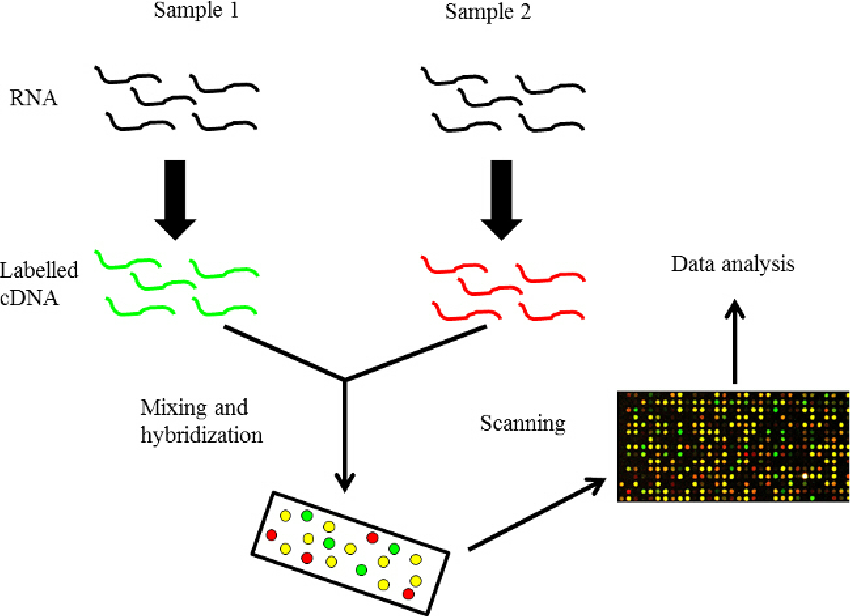
\includegraphics[width=0.8\textwidth]{MicroArray.png}
		\caption{A picture showing the creation of microarray datasets \cite{afzal2015fast}.}
		\label{fig:MicroArray}
	\end{figure}
	
	% Challenges
	Micro-array data is known to present challenges in data quality and needs normalisation for the data to be useful \cite{selvaraj2011microarray}. The thousands of features that are based in the data also indicate that feature selection is very important, so the irrelevant genes can be removed. Aside from that, size may also be an issue. Due to the sheer size of the data not all analyses will perform optimally in both time and quality. In this research two microarray datasets are used for research:
	
	\begin{itemize}
		% Psoriasis
		\item \textit{Psoriasis microarray dataset} \\ This dataset is comprised of five different data sets \cite{nair2009genome, suarez2012expanding, bigler2013cross, yao2008type}. These five different datasets consist of 54675 features, all corresponding to gene expression. Samples were collected from three different test subject groups: affected skin from test subjects suffering from psoriasis (214 samples), unaffected skin from test subjects suffering from psoriasis (209 samples) and skin from healthy test subjects (85 samples). Combining these three sample types gives 508 samples. Since the data comes from five different experiments, the data is normalized for every experiment.
		% Cancer
		\item \textit{Arcene: Cancer microarray dataset} \\ This dataset, called Arcene dataset, is used in a challenge focussing on classification problems with a low number of samples, but a high number of features \cite{wojnarski2010rsctc}. It consists of the same number of features as the Psoriasis data set, 54675 features corresponding to gene expression. It also has 383 samples corresponding to nine different test subject groups. The challenge did not provide labels for the test subject groups. Also these groups differ in size, one group corresponding to 150 samples and the others varying from 16 to 47 samples.
	\end{itemize}
	
	\subsection{Mass Spectrometry Datasets}
	\label{PLsubsec:MassSpect}
	
	Mass spectrometry data contains information on proteins and peptides \cite{cottrell1999probability, dettmer2007mass}. Analysis of this information is used in studies about proteins, also known as proteomics \cite{matthiesen2008analysis}. Mass spectrometry is a technique that can be used to find how much of a certain protein is present. This is done by measuring the mass of gas-phase ions originating from molecules of that protein, showing that protein is present. On top of that it can also measure the quantity of the mass, therefore showing how much of a protein is present \cite{watson2007introduction}.
	
	\begin{figure}
		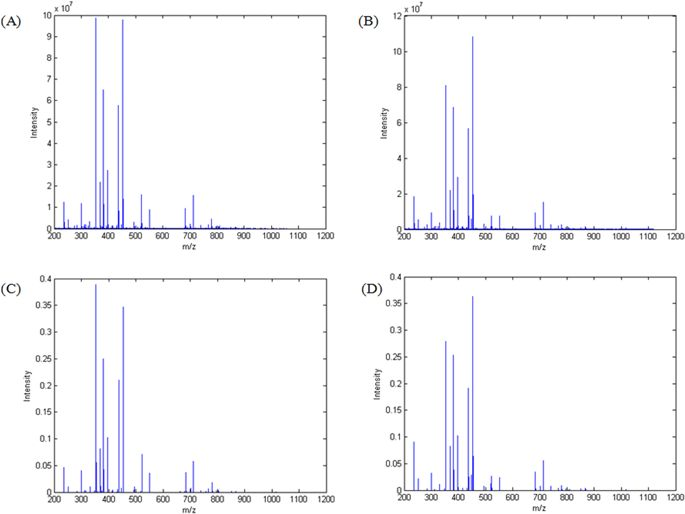
\includegraphics[width=\textwidth]{MassSpect.jpg}
		\caption{Four example figures of the data created by mass spectrometry. The measured molecule masses correspond to the peaks in the figures \cite{neves2018mass}.}
		\label{fig:MassSpect}
	\end{figure}
	
	
	% Challenges
	Challenges in the analysis of mass spectrometry datasets are mainly found in the way this data is produced. The expression is given for several proteins and this expression can differ significantly between proteins. Therefore some type of normalisation is useful. Aside from that, in this technique usually a high number of proteins is tested at the same time. Therefore feature selection can be helpful to remove irrelevant genes. Two mass spectrometry datasets were used in this research:

	\begin{itemize}
		\item \textit{RSCTC: Cancer mass spectrometry dataset} \\ This dataset, called RSCTC dataset, was created as a classification problem to distinguish cancer patterns from normal patterns \cite{NIPS2004_2728}. It is created for the 'Neural Information Processing Systems' conference by merging three mass spectrometry datasets. It consists of 10000 features corresponding to either spectra of the mass spectrometry or probe variables without any predictive power. Samples from two groups are taken, from patients with ovarian or prostate cancer and from control patients. No labels are given to the groups, however it is known that one of the groups has 88 samples and the other 112 samples, combined in a total of 200 samples.
		% MicroOrganisms
		\item \textit{Micro organisms mass spectrometry dataset} \\ This dataset is created to back up a proposed method for routinely performing direct mass spectrometry based bacterial species identification \cite{doi:10.1093/bioinformatics/btu022}. It consists of 1300 features corresponding to different spectra of the mass spectrometry data and 20 test subject groups corresponding to Gram positive and negative bacterial species. Gram classification is a result of a Gram stain test \cite{madigan2017brock}. The groups differ in size varying from 11 to 60 samples, making a total of 571 samples.
	\end{itemize}
		
	%\subsubsection{Nuclear Magnetic Resonance Datasets}
	% \cite{capitani2017nuclear}
	
	\subsection{Clinical Datasets}
	\label{PLsubsec:Clinical}
	
	% Introduction
	Clinical datasets originate from clinical research \cite{liu2012data, sittig2008grand}. In clinical research data is created to determine the effectiveness of treatments in the hospital, for example for a drug \cite{pocock2013clinical}. The values in clinical datasets can originate from blood tests \cite{bendele1999efficacy}, but can also be data derived from other fluids or tissues of the body.  
	
	% Challenges
	The clinical datasets that are analysed by data analysts usually are created by doctors and laboratory researchers. This sometimes causes mismatches between the data and the goals of the biomedical engineer working with the data. Main challenges are the bias in the data due to difference in focus of the doctors, therefore having misrepresentation of certain patients. Often values are missing in the data and errors are present due to humans entering those values \cite{pocock2013clinical}. At last, the number of samples that can be gathered is usually limited, due to the clinical trials being limited to the number of patients present. Three clinical datasets are used in this research:
	
	\begin{itemize}
		\item \textit{Heart Attack Echo-cardiogram dataset} \\ For this dataset patients were selected, who at one point in their lives suffered a heart attack and survived \cite{kan1986short}. A prediction model can be made that models the months of survival after the heart attack as the prediction variable. There are 9 features for 108 samples present, with a total of 97 missing values. Every feature but two have at least one missing value, but by far the most missing values are located in the feature "alive-at-1" (still alive after 1 year) with 58 missing values and 54\% of total number of samples. This high number of missing values can be partially explained because of lack of documentation, partially because no year had passed, yet, after data distribution. % HeartAttackEcho - https://www.openml.org/d/222 & https://heart.bmj.com/content/56/5/422.short (no access)
		\item \textit{Hepatitis dataset} \\ The mortality rate of hepatitis was tested using 19 features over 155 samples \cite{diaconis1983computer, cestnikkononenkoj}. Two class types are distinguished as "died" and "lived" with thirteen boolean and six numeric attributes. The total number of missing values is 167 spread over 15 classes, with the feature labelled "histology" having the majority of 67 missing values. Two previous articles were written, using this dataset as an example for their methods \cite{diaconis1983computer, cestnikkononenkoj}.
		% Hepatitis - https://www.openml.org/d/55 (source unknown)
		\item \textit{Primary Biliary Cirrhosis dataset} \\ Patients were classified in three groups in this dataset: alive, transplanted and dead \cite{murtaugh1994primary}. 18 features are present in the dataset: one date-specific, two categorical, five boolean and ten numeric attributes. The dataset consists of 1945 instances and 1133 missing values. The missing values are distributed over six features, the feature \textit{serum\_cholesterol} having 821 and the other five around 60 missing values. The missing values are noted as most likely not missing completely at random. % Cirrhosis -  https://aasldpubs.onlinelibrary.wiley.com/doi/abs/10.1002/hep.1840200120
	\end{itemize}
	
	\subsection{Survey Datasets}
	\label{PLsubsec:Survey}
	
	% Introduction
	Whereas opinions are divided whether biomedical surveys can be seen as clinical data \cite{misery2011sensitive}, in this report they are mentioned separately. Survey data simply consists of answers to biomedical questions. Patients answer questions related to some kind of biomedical subject for analysis. Due to the simple way of conducting such a survey, many patients can fill out the questionnaire and therefore many samples are created.
	
	% Challenges
	Challenges in surveys mainly consists of errors in filling out the answers. The patients' answers can be very subjective, possibly creating bias. Also human errors are present when filling out surveys, as well as accidentally or purposely refusing to fill out an answer. One survey dataset was used in this research:
	
	\begin{itemize}
		\item \textit{Cervical Cancer dataset} \\ This dataset is consisting of 858 samples and is based on the increased risk of subjects becoming cervical cancer patients \cite{fernandes2017transfer}. Since a risk can be fairly subjective, four aspects were used to determine whether an increased risk is present or not: two doctors, a cytology examination and a biopsy examination. For analysis a new increased risk factor was made by giving each subject a value in $[0, 4]$, implying the number of times this subject has been classified as an increased risk subject. The dataset consists of 31 features, 24 boolean and numeric features originated from a survey and 7 boolean and numeric features originated from the hospital. A total of 3622 values are missing of which 787 times the hospital features "STDs: Time since first diagnosis" and "STDs: Time since last diagnosis" caused by no sexually transmitted disease (STD) ever being present. All other missing values originate from subjects not answering survey questions, the "Age" feature being the only survey question that was always answered.
	\end{itemize}
	
	\subsection{Data Symbols}
	\label{subsec:DataSymbols}
	
	Often in this research project, equations and pseudo-algorithms are discussed. In these equations and pseudo-algorithms, several symbols were used to explain the data. A quick overview of these symbols is given (Table \ref{tab:DatasetSymbols}) as well as a more detailed description:
	
	\begin{itemize}
		\item \textit{$F$} -
		A list that contains all the names of the features. It is a list of size $m$ with $m$ being the number of features. A subset $x$ of $F$ is written as $F_x$.
		\item \textit{$S$} -  
		A list of all samples in a dataset. It is a list of size $n$ with $n$ being the number of samples. A subset $x$ of $S$ is named $S_x$ and a single sample is usually called $s$. 
		\item \textit{$X$} -
		A matrix that contains all sample values for every feature. It is an $n$ by $m$ matrix with $n$ being the number of samples and $m$ being the number of features. If the values of a specific feature $f$ or a subset of features $F_x$ are used this is written as $X_f$ and $X_{F_x}$ respectively, hence the column $f$ or columns $F_x$ are selected. Similarly for $X_s$ and $X_{S_x}$ the row $s$ or rows $S_x$ respectively are collected from $X$.
		\item \textit{$y$} -
		A vector that contains all class labels for every sample. It is a vector of size $n$ with $n$ being the number of samples.
		\item \textit{$W$} - 
		Weights given to a feature after training a feature selection technique. The weight of feature $f$ or set of features $F_x$ is called $W_f$ and $W_{F_x}$ respectively.
	\end{itemize}
	
	\begin{table}[]
		\caption{An overview of the symbols used to explain the data}
		\label{tab:DatasetSymbols}
		\begin{tabular}{|l|l|}
			\hline
			\textbf{Value} & \textbf{Description}                                   \\ \hline
			$m$				 & The number of features                                 \\ \hline
			$F$              & A list of ($m$) features                                 \\ \hline
			$n$				 & The number of samples                                 \\ \hline
			$S$              & A list of ($n$) samples                                  \\ \hline
			$X$              & A matrix of ($n \times m$) dataset values \\ \hline
			$y$              & A vector of ($n$) output labels                          \\ \hline
			$W$              & A list of feature weights                              \\ \hline
		\end{tabular}
	\end{table}
	
	
	\section{Software}
	\label{PLsec:Software}
	
	% Introduction
	For this research one programming language is used, \textit{Python} version 3.6. This language was chosen, due to the numerous possibilities in preprocessing and analysis in the open source language \cite{mckinney2010data} (Appendix \ref{app:BiomedicalDataAnalysis}). \textit{Python} makes use of packages containing additional classes and methods to be used in experiments. To easily import these packages the \textit{Anaconda} version 3 environment is used \cite{yan2018hands}. Packages available by \textit{Anaconda} and often used in the analyses are:
	
	\begin{itemize}
		\item \textit{NumPy} \cite{walt2011NumPy} \\
		\textit{NumPy} provides data structures efficient in use for data analysis. On top of that it also provides multiple methods to alter and preprocess these data structures, improving data analysis efficiency significantly.
		\item \textit{SciPy} \cite{jones2014SciPy} \\
		\textit{SciPy} provides analysis methods, mainly focused on statistics. These methods are compatible with the \textit{NumPy} data structures and provide a way to simply perform statistical analyses.
		\item \textit{Scikit-learn} \cite{pedregosa2011scikit} \\
		\textit{Scikit-learn}, also known and shortened as \textit{sklearn}, is focused around machine learning. It provides numerous simple machine learning algorithms as well as several other algorithms and classes that are often used in analysis, such as preprocessing methods and environment testing creation.
		\item \textit{Pandas} \cite{mckinney2012Python} \\
		\textit{Pandas} is also used in parts of this research. \textit{Pandas} creates a very intuitive way of distributing data, presenting datasets that are easy to understand for users and in analysis. It is an overlay of the \textit{NumPy} data structure and often used in \textit{Python}.
	\end{itemize}
	
	Two other packages were used in this research that are not part of \textit{Anaconda}. These packages have to be downloaded separately:
	
	\begin{itemize}
		\item \textit{TPOT} \cite{olson2016tpot} \\
		\textit{TPOT} is an abbreviation for "Tree-based Pipeline Optimization Tool" and uses automated machine learning to find the best machine learning pipeline. It makes use of several other packages, such as the \textit{NumPy}, \textit{SciPy} and \textit{Scikit-learn}, all of these being available in \textit{Anaconda}.
		% Should this be 
		\item \textit{metalearn} \\
		\textit{metalearn} is a package that computes meta-features (Appendix \ref{app:MetaFeatures}) for datasets. These meta-features can be used for further analysis or can give a direction for further analysis. \textit{metalearn} uses packages available in \textit{Anaconda}, as well, such as \textit{NumPy}, \textit{SciPy}, \textit{Scikit-learn} and \textit{Pandas}.
	\end{itemize}


	\section{Concepts}
	\label{PLsec:Concepts}
	
	Several concepts occur in more than one of the three research chapters. These concepts are explained in this section to avoid overlap:
	
	\begin{itemize}
		\item \textit{Cardinality} \\
		The cardinality of features is the number of unique options available. For categorical and ordinal data it is the total number of categories and for numeric data it is every unique numeric value.
		\item \textit{Correlation} \\
		Correlation computes the expressibility of two variables in regard to each other. A variable is relevant if it can predict the outcome of the another variable. One way of computing this relevance for a variable $x_i$ of feature $i$ with mean $\bar{x }_i$ and target variable $y_i$ with mean $\bar{y}_i$ is by using the linear correlation coefficient $r$, also known as Pearson' correlation \cite{yu2003feature} (Equation \ref{eq:Correlation}). The correlation filter methods mainly works for continuous data, but can also be used for discrete data \cite{hall2000correlation}.
		
		\begin{equation}\label{eq:Correlation}
		r(x,y) = \frac{\sum_{i}(x_i - \bar{x}_i)(y_i -\bar{y}_i)}{\sum_{i}(x_i - \bar{x}_i)\sum_{i}(y_i -\bar{y}_i)}
		\end{equation}
		
		\item \textit{Cross validation} \\
		Cross validation is a model validation technique. A dataset is split in two groups: training and validation data. The training data is used for training the algorithm and the validation data is used for validating it. Splitting the data can only be done once, but also more times to create multiple folds. Multiple types of cross validation are known, examples are k-fold cross validation, bootstrapping and leave-one-out \cite{kohavi1995study}.
		\item \textit{Leave-one-out} \\
		Leave-one-out is a type of cross validation. For a dataset of size $n$, $n$ times the data is split into a training set of $n-1$ samples and a validation set of the other $1$ sample. All samples are in the validation set exactly onece. The algorithm is then trained and validated for the $n$ splits and the validation scores are averaged. This way the validation score is found while using as much training data as possible \cite{kearns1999algorithmic}. 
		\item \textit{Data types} \\
		% Numeric, categorical and ordinal features
		Feature values can be of multiple types, for example: numbers, text, dates and other possibilities. The usefulness of these types can differ between analysis, showing that not all techniques are suitable for a dataset. Usually all of these types are put in one of these three groups:
		\begin{itemize}
			\item \textit{Categorical data}: This type of data splits the features into different categories, giving a finite number of options for the feature values. These categories are usually text-based and lack special relations between them, such as an ordering \cite{agresti2003categorical}. 
			\item \textit{Numeric data}: Features that have numbers as values that originate from a predefined range are of the numeric type. Numeric values can be ordered. Also the cardinality (number of distinct feature values) usually is much higher for numeric data \cite{edwards2002explaining}. 
			\item \textit{Ordinal data}: Ordinal data are in between categorical and numeric data. Ordinal features have multiple predefined categories that have some kind of ordering. The number of categories usually is very low, giving the outcome a low cardinality \cite{han2011data}. Ordinal data are harder to define as a data type, due to the lack of ordering in text based values and the lack of possibilities in defining only a finite number of categories in numerical data. Therefore usually the most suitable of categorical data and numerical data is chosen and ordinal data are transformed to that type.
		\end{itemize}
		\item \textit{Dimensionality} \\
		The dimensionality of a dataset in literature is the number of features of that dataset\cite{yu2003feature,lim2003planar,biesiada2007feature}. A high dimensionality therefore indicates a high number of features. The package \textit{metalearn} calls dimensionality the number of features divided by the number of instances. If this definition of dimensionality is used it is specifically stated. This definition is used to show possible imbalance between the number of features and instances and normally the dimensionality should be very low, at least $<1$.
		\item \textit{Experiment set-up} \\
		When doing machine learning experiments, a set-up is made that takes into account training the data, validating the result of the training and testing the data set with separate data. The tests are exectured with a to be trained algorithm and a scoring function that shows the quality of the trained algorithm. Three phases are present during the experiment:
		\begin{itemize}
			\item \textit{Splitting the data} \\
			The data is split into a training set and test set at the start, usually more than 75\% of the data is chosen to be in training set. The training set is split in training data and validation data. This usually is done by cross validation or leave-one-out. 
			\item \textit{Training and validation} \\
			The algorithm is trained by giving it the training data. Afterwards with the validation data a score is computed for how well the algorithm can predict the validation data. Since with cross validation and leave-one-out multiple combinations of training and validation data are made, the algorithm is separately trained and validated multiple times. The separate validation scores are combined to one validation score, usually by averaging all of them. This validation score then shows how well the algorithm trained by the training set would perform on the training data.
			\item \textit{Testing the algorithm} \\
			Since also new data should be tested on the algorithm, at last the initially created test set is used. A score is computed on how well the algorithm, trained on the complete training set, can correctly predict the test data. This data that has no direct relation with the training data shows how well the algorithm performs when new data is present.
		\end{itemize}
		\item \textit{Hot encoding}:\\
		One-hot encoding is the actual name, but in the report it is called hot encoing. Hot encoding is used when numerical and categorical values are combined in the dataset. Whereas numerical features have numbers as values, categorical features usually correspond to text with no clear order. Hot encoding is used to give numerical values to categorical features. This is done by creating a new separate feature for every category and differ the values between presence of this category (e.g. the feature value becomes $1$) and absence of this category (e.g. the feature value becomes $0$). An example would be for a patient either undergoing treatment 'A', 'B' or 'C'. The categorical feature 'treatment' then has the options {'A', 'B', 'C'}. After hot encoding the 'treatment' feature is replaced by features 'treatment A', 'treatment B' and 'treatment C', and the values of these features are either $1$ if that treatment is performed or $0$ if that treatment is not performed. This way no ordering is present for the categorical data.
		% Mutual information
		\item \textit{Mutual information} \\
		Mutual information can be used on two different variables. The relevance of using one variable to predict the other variable is used in the equation to compute mutual information (Equation \ref{eq:MutualInformation}). In this equation the probability density function $p$ is used to find the mutual information (MI) between variables $x$ and $y$ \cite{peng2005feature}. Mutual information can be used for both classification and regression. It was initially meant for use in communication channels, however its statistical decision making capabilities made it a good filter method \cite{battiti1994using}.
		
		\begin{equation}\label{eq:MutualInformation}
		MI(x, y) = \sum_x \sum_y p(x, y) \log{\frac{p(x, y)}{p(x)p(y)}}
		\end{equation}
		
		
		\item \textit{Normalisation}:\\
		The difference in value size between numerical features can differ greatly. For example, if both the length of a patient's body and finger are measured, the value of body length is much bigger than the value of finger length. On top of that the variance in the features body length and tongue length differ in size, too. To prevent this potential bias in data analysis, all features are normalized on both mean and variance. This normalisation is usually done in two steps for a feature with mean $\mu_0$ and standard deviation $\sigma_0$: Step one is changing to a mean value $\mu_1$ with value $\mu_1 = 0$ by subtracting all values by the mean $\mu_0$. Step two is to divide all features by the standard deviation $\sigma_0$, so the new standard deviation $\sigma_1$ becomes $\sigma_1 = 1$.
		\item \textit{Scoring functions} \\
		% Accuracy, Precision, Recall, F1-score, Cohen's kappa.\\
		This quality of an algorithm in machine learning is measured with a scoring function. Three of these scoring functions are explained. They are defined in terms of true and false positives (TP and FP respectively) and true and false negatives (TN and FN) and in these discussions $n$ is the size of the test set.
		\begin{itemize}
			\item \textit{Accuracy} \\
			The simplest and most used approach to measure quality is by using accuracy. This is usually the choice when no imbalance is present and there is no specific focus in results. Accuracy is simply the ratio of correctly classified samples and all classified samples (Equation \ref{eq:Accuracy}). So for a test set of 30 samples, if 6 samples are incorrectly classified the accuracy would be $24/30 = 0.8$. 
			
			\begin{equation}\label{eq:Accuracy}
			\text{accuracy} = (TP + TN) / (TP + FP + TN + FN)
			\end{equation}
			
			\item \textit{F1 score} \\
			The accuracy assumes there is no difference in output categories. If the output is unbalanced and majority and minority classes exist, another approach can be used called the F1 score. The F1 score treats classes equally by computing the precision and recall and combining those as a harmonic mean. Precision shows the portion correctly classified out of all positively classified (Equation \ref{eq:Precision}) and recall shows the portion correctly positively classified out of all positive values (Equation \ref{eq:Recall}). After that both are balanced in the F1 score by computing a harmonic mean of precision and recall (Equation \ref{eq:F1}). Therefore F1 evaluates both FP and FN evenly. Precision and recall are also sometimes used if one of the false classifications FP and FN is more important than the other.
			
			\begin{equation}\label{eq:Precision}
			\text{precision} = TP / (TP + FP)
			\end{equation}
			
			\begin{equation}\label{eq:Recall}
			\text{recall} = TP / (TP + FN)
			\end{equation}
			
			\begin{equation}\label{eq:F1}
			\text{F1} = 2 \frac{\text{precision} \cdot \text{recall}}{\text{precision} + \text{recall}}
			\end{equation}
			
			\item \textit{Cohen's kappa} \\
			Cohen's kappa $\kappa$ is a statistical approach for a quality label. $\kappa$ shows the agreement between the result $p_0$ (for example the aforementioned accuracy) and compares this with the expected agreement by chance $p_e$ (Equation \ref{eq:Kappa}) It is mainly used if the output can be two classes \cite{blackman2000interval} and does not take into account random classification. Therefore it gives a better indication of the effectiveness.
			
			\begin{equation}\label{eq:Kappa}
			\kappa = \frac{p_0 - p_e}{1 - p_e} = \frac{2(TP \cdot TN - FP \cdot FN)}{(TP + FP) \cdot (TN + FN) + (TP + TN) \cdot (FP + FN))}
			\end{equation} 
		\end{itemize}
		\item \textit{Standardisation} \\
		Standardisation is an alternative to normalisation, a technique to use when value sizes differ greatly between numerical features. Normalisation is based on changing values to a $[0, 1] $ range. The minimum value is changed to $0$, the maximum value to $1$ and all values in the middle are changed accordingly to fit the range $[0, 1]$. 

	\end{itemize}
	
	
	\chapter{Feature Selection}
	\label{chap:FeatureSelection}
	
	\section{Introduction}
	\label{FSsec:Introduction}
	
	% Topic dimensionality reduction
	For a biomedical engineering framework dimensionality reduction is important.  Some biomedical datasets contain a high number of features, whereas only a selection of those features are interesting. A direct link of features to the output is desired, therefore especially dimensionality reduction based on feature selection is important. Multiple projects attempted to reduce the number of features \cite{baumgartner2006data, welthagen2005comprehensive} which resulted in multiple algorithm proposals \cite{lim2003planar, peng2010novel, biesiada2007feature, ding2005minimum} and tests on their performance \cite{catal2009investigating, liu2002comparative}. Basic feature selection algorithms should be present in the framework and are therefore tested on the available data sets. The research goal is \emph{to evaluate the performance of feature selection methods and make a choice on which methods should be added to the framework}. In this document several of those algorithms are presented and test their quality.
	
	\newpage
	\section{Background}
	\label{FSsec:Background}
	
	% Introduction background & layout background
	Before testing several feature selection methods, first the background of the study is explained. Firstly, the datasets and their characteristics are explained. Secondly, feature selection methods are discussed. Thirdly the concept automated machine learning is discussed as a possible technique to add to the framework, combined with a tool that implements automated machine learning.
	
	\subsection{Datasets}
	\label{FSsubsec:Datasets}
	
	% Data sets	
	Four datasets were used as a case study for the feature selection algorithms (Subsection \ref{PLsec:Datasets}). Two sets are microarray datasets that are used for research on psoriasis \cite{nair2009genome, suarez2012expanding, bigler2013cross, yao2008type} and cancer \cite{wojnarski2010rsctc}. Two other sets are mass spectrometry data sets, used for research on cancer \cite{NIPS2004_2728} and micro organisms \cite{doi:10.1093/bioinformatics/btu022} (Subsection \ref{PLsec:Datasets}). These four datasets all have a high number of features varying from 1300 to 54675 features with a number of samples varying from 200 to 580 samples (Table \ref{tab:DataSetDescriptions}). All of these datasets are based on classification as tests are done for different test subject groups, therefore the focus on feature selection algorithms will also be based on classification. Many features are expected to be irrelevant in this classification and therefore could be removed with feature selection.	

	\begin{table}[]
		\centering
		\caption{A schematic overview of the four datasets.}
		\label{tab:DataSetDescriptions}
		\begin{tabular}{ll|llll}
			\textbf{Dataset focus} & \textbf{Data type}                                          & \textbf{Features} & \textbf{Samples} & \textbf{Classes} & \textbf{Remarks}                                                                                                        \\ \hline
			Psoriasis        & Micro-array                                                 & 54675             & 580              & 3                & \begin{tabular}[c]{@{}l@{}}- Derived from five \\ different datasets \cite{nair2009genome, suarez2012expanding, bigler2013cross, yao2008type} \\ -- \end{tabular}                                       \\
			Cancer           & Micro-array                                                 & 54675             & 383              & 9                & \begin{tabular}[c]{@{}l@{}}- Used in a data \\ mining challenge \cite{wojnarski2010rsctc}\end{tabular}                                            \\ \hline
			Cancer           & \begin{tabular}[c]{@{}l@{}}Mass\\ Spectrometry\end{tabular} & 10000             & 200              & 2                & \begin{tabular}[c]{@{}l@{}}- Created for the \\ NIPS conference \cite{NIPS2004_2728}\\ - Several probe \\ features are present \\ -- \end{tabular} \\
			Micro-organisms  & \begin{tabular}[c]{@{}l@{}}Mass\\ Spectrometry\end{tabular} & 1300              & 571              & 20               & \begin{tabular}[c]{@{}l@{}}- Originates from a \\ micro organisms study \cite{doi:10.1093/bioinformatics/btu022}\end{tabular}                                                                                                                       
		\end{tabular}
	\end{table}
	
	\subsection{Feature Selection Methods}
	\label{FSsubsec:FeatureSelectionMethods}
	
	% Introduction feature selection
	Feature selection is a way to perform dimensionality reduction. In feature selection a subset of features is chosen to represent the complete sample space \cite{Guyon2006}. Several techniques are available to choose a representation subset and the effectiveness of these techniques has been tested multiple times \cite{CATAL20091040, molina2002feature, chandrasheto split bykar2014survey}. These techniques can be grouped accordingly in three different categories: \textit{filter methods}, \textit{wrapper methods} and \textit{embedded methods} \cite{saeys2007review}. Each of these methods is explained in what follows. For better understanding of the different feature selection methods, pseudo-algorithms are created for each of them.
	
	% Preprocessing
	Before actually performing feature selection, usually some kind of preprocessing is done. This preparation consists of making the data adequate for feature selection to be possible as well as preprocessing, such that all features are processed evenly. Therefore normalisation of numerical values is done and possible hot encoding if categorical features are present. 
	
	\subsubsection{Filter Methods}
	\label{FSsubsec:FilterMethods}
	
	% Introduction filter methods
	Filter methods are based on giving relative ranks to the features in a feature space. All features are given a value based on their performance and are ranked by those values \cite{Duch2006, saeys2007review}. Several methods are used to rank the features. These methods are usually based on splitting data matrix $X$ twice. First they are split by feature ($X_{f_1}, X_{f_2} ... X_{f_n}$) for computation. Secondly the columns are split by output classes $c_1, c_2 ... c_n$ ($X_{f}^{c_1}, X_{f}^{c_2} ... X_{f}^{c_p}$) to distinguish the predictive power for features between classes. A ranking method would quantify the significance according to these values. This results in ranking method $R(X_f, y)$ in which sample label $y$ is used to split the data per class. For illustration a ranking method collection is given:
	
	\begin{itemize}
		% T-test binary
		\item \textit{T-test and ANOVA} \\ 
		Statistics can be used to compare groups with each other. In statistics these groups are seen as separate distributions, which may or may not be seen as independent distributions. If there are two groups  a t-test can be done to find the chance for these groups to originate from the same distribution \cite{heiberger2004statistical} (Appendix \ref{app:BiomedicalDataAnalysis}). 
		For sample classifications the groups would consist of samples with the same label ($X_{f}^{c_1}$  and $X_{f}^{c_2}$). For example, the t-test can be done between group with class $c_1$ and group with class $c_2$. If the values of a certain feature from these groups are highly unlikely to follow the same distribution ($R(X_{f}^{c_1}, X_{f}^{c_2})$), the p-value will be very low and therefore the rank will be higher.
		
		If there are more than two groups that must be checked whether they are from the same distribution ($R(X_{f}^{c_1}, X_{f}^{c_2} ... X_{f}^{c_p})$, a t-test cannot be used. In this case the option is available for a multiple group testing, also called analysis of variance (ANOVA). ANOVA computes whether not only two, but multiple groups can originate from the same distribution. ANOVA needs equal group sizes, otherwise the results of the tests are less reliable. The less powerful Kruskall Wallis test can be used if this reliability is needed. Another disadvantage is that t-test and ANOVA should only be used if the groups follow a normal distribution, which might not be the case (Appendix \ref{app:BiomedicalDataAnalysis}) \cite{heiberger2004statistical}.
		
		% Mutual information
		\item \textit{Mutual information} \\
		Mutual information is another way of matching features with the results. The relevance of using one variable to predict the other variable is used in the equation to compute mutual information. 
		
		% Correlation
		\item \textit{Correlation} \\
		Correlation, similarly to mutual information, computes the expressibility of two variables for each other. A variable is relevant if it can predict the outcome of the target variable.
		
	\end{itemize}
	
	% Feature selection threshold criteria
	These ranking methods $R$ to rank the features are only the first step in the filter methods. The next step is choose which features to filter out based on $R$. A quick approach would be to choose a number or fraction $n$ and select the top $n$ ranked features from the complete space (Algorithm \ref{alg:FilterTopNAlgorithm}). Another approach would be to use thresholds derived from literature \cite{donoho2008higher} (Algorithm \ref{alg:FilterAlgorithm}). For the t-test, a p-value of $0.05$ is often chosen as the threshold value \cite{storey2003statistical, higgins2003measuring}.
	
	\begin{algorithm}[H]
		\caption{A basic top $n$ filter algorithm \cite{Duch2006}}\label{alg:FilterTopNAlgorithm}
		\begin{algorithmic}[1]
			\Procedure{FilterSelection($X, y, F, R, n$)}{}
			\State $F_{\textit{selected}} \gets \O$ 	\Comment{Start with empty feature set}
			\State $Z \gets \O$							\Comment{Start with empty set of ranking values}
			\For {$f \textbf{ in } F$} 					\Comment{For all features in $F$}
			\State $Z_f \gets R(X_f, y)$ 				\Comment{Compute the ranking value between feature and output} 			
			\State $Z \gets Z \cup \{Z_f\}$ 				\Comment{Add the ranking value to the set of ranking values}
			\EndFor
			\State $\textbf{Sort } F \textbf{ by } Z$ \Comment{Sort the features by their ranking value}
			\State $F_{}selected \gets F_{[1,n]}$ \Comment{Select the top n features from the sorted feature set}
			\State $\textbf{return } F_{\textit{selected}}$
			\EndProcedure
		\end{algorithmic}
	\end{algorithm}	
	
	\begin{algorithm}[H]
		\caption{A basic filter algorithm \cite{Duch2006}}\label{alg:FilterAlgorithm}
		\begin{algorithmic}[1]
			\Procedure{FilterSelection($X, y, F, R, \alpha$)}{}
			\State $F_{\textit{selected}} \gets \O$ 	\Comment{Start with empty feature set}
			\For {$f \textbf{ in } F$} 					\Comment{For all features in $F$}
			\If {$\text{R}(X_f, y) > \alpha$}			\Comment{Check if ranking value is higher than threshold $\alpha$}
			\State $F_{\textit{selected}} \gets F_{\textit{selected}} \cup \{f\}$ \Comment{Add $f$ to selected features}
			\EndIf
			\EndFor
			\State $\textbf{return } F_{\textit{selected}}$
			\EndProcedure
		\end{algorithmic}
	\end{algorithm}
	
	% Advantages, disadvantages filter methods	
	Using filter methods has its advantages and disadvantages. These filter methods are very computationally efficient. Every feature is given a value for its rank and then a subset is selected based on those ranks. These filter methods however do not take into account dependencies between features. These dependencies could make the final feature subset worse, as maybe some features are related. Other methods are better at handling those dependencies \cite{Duch2006, saeys2007review}.
	
	\subsubsection{Wrapper Methods}
	\label{FSsubsec:WrapperMethods}
	
	% Introduction wrapper methods
	Filter methods take into account the direct relation between features and the output classes, whereas wrapper methods focus more on the subsets of features and their ability to classify the data. Wrapper methods try to find the best combination of features to classify the given data and take into account the change when adding or removing features from a candidate subset. The choice of subset selection is "wrapped"  around the quality computation, therefore this method is called a wrapper method \cite{Reunanen2006}. Since an exhaustive search of trying out all possible subsets would span a computation time of $2^n$ with $n$ being the number of features \cite{Alsallakh2016PowerSet}. This combinatorial explosion should be avoided and therefore less computationally intensive approximation concepts have been constructed. Three of those concepts are explained, focusing on basic sequential search, extensions of sequential search and stochastic search.
	
	% Evaluation method
	Before explaining the possible wrapper methods, first the evaluation function $J$ should be discussed. To find out which subset of features can classify the data the best way, a function should be used to evaluate the performance of the subset \cite{Reunanen2006}. Evaluation functions can be based on conditional independence \cite{Reunanen2006,tsamardinos2017massively}, showing the difference in performance for a subset with and without a certain feature. Other evaluation functions are based on machine learning techniques \cite{huang2013automated, saeys2007review}, rating the ability to classify the outcome. Several interesting approaches for evaluation functions are shown in maximum relevance, minimum redundancy algorithms \cite{SENAWI201747, el2009new, radovic2017minimum} (MRMR algorithms). In these MRMR algorithms, several different evaluation functions are used based on the ability of features to classify the outcome (relevance) and the presence of correlation between features (redundancy). In this project, the evaluation function is fixed on the machine learning algorithm Naive Bayes, due to its understandability.
	
	\begin{itemize}
		% Sequential search
		\item \textit{Sequential search} \\
		The first concept to be explained is sequential search. This wrapper method tries to improve a candidate subset by evaluating the change of the sequential addition or removal of a specific feature. Therefore, two types of sequential search are possible, known as forward selection and backward selection. Forward selection starts with the empty subset. Every feature is iteratively evaluated and added to the feature subset if the evaluation function shows an increase in prediction. A maximum feature subset selection size $l$ can be defined if needed, as well. The layout of forward selection is shown as a pseudo algorithm (Algorithm \ref{alg:ForwardSelection}) for understanding \cite{Reunanen2006}.
		
		% Backward selection
		Backward selection does the opposite of forward selection. It starts with the complete feature set in which every feature is iteratively evaluated by the evaluation function for its contribution. If the evaluation function shows that its contribution is very small, it is removed. This way only features with a high impact will remain in the subset. The maximum number features that can be removed $r$ can be defined if needed, as well. be A layout of backward selection is shown as a pseudo algorithm (Algorithm \ref{alg:BackwardSelection}) for understanding, as well \cite{Reunanen2006}.
		
		% Order discussion
		In both forward and backward selection the sequence order is important. Different feature subsets will be made for different order of features. The ordering can be changed in a specific way if needed. Examples would be using the ranking concepts used by filter methods. Another possibility would be to randomize the order and run the algorithm multiple times to find the best subset \cite{Reunanen2006}.
		
		% Insert pseudo-algorithm for forward and backward sequential search
		\begin{algorithm}[H]
			\caption{A forward selection sequential search algorithm \cite{Reunanen2006}}\label{alg:ForwardSelection}
			\begin{algorithmic}[1]
				\Procedure{SequentialForwardSelection($X, y, F, J, \alpha, l$)}{}
				\State $F_{\textit{selected}} \gets \O$				\Comment{Start with empty feature set selection}
				\For {$f \textbf{ in } F$}							\Comment{For all features in $F$}
				\If {$J(X_{F_\textit{selected}}, y, X_f) > \alpha$}	\Comment{Check if evaluation is higher than $\alpha$ with feature $f$}
				\State $F_{\textit{selected}} \gets F_{\textit{selected}} \cup \{f\}$	\Comment{Add $f$ to the feature set selection}
				\EndIf
				\If {$\text{length}(F_{\textit{selected}}) = l$}	\Comment{Stop if size of feature set selection has been reached}	
				\State $\textbf{break}$
				\EndIf
				\EndFor
				\State $\textbf{return } F_{\textit{selected}}$
				\EndProcedure
			\end{algorithmic}
		\end{algorithm}
		
		\begin{algorithm}[H]
			\caption{A backward selection sequential search algorithm \cite{Reunanen2006}}\label{alg:BackwardSelection}
			\begin{algorithmic}[1]
				\Procedure{SequentialBackwardSelection($X, y, F, J, \alpha, r$)}{}
				\State $F_{\textit{selected}} \gets F$				\Comment{Start with complete feature set selection}
				\For {$f \textbf{ in } F_{\textit{selected}}$}		\Comment{For all features in $F_{\textit{selected}}$}
				\If {$J(X_{F_{\textit{selected}} \backslash \{f\}} , y, f) < \alpha$} \Comment{Check if evaluation is higher than $\alpha$ without $f$}
				\State $F_{\textit{selected}} \gets F_{\textit{selected}} \backslash \{f\}$ \Comment{Remove $f$ from the feature set selection}
				\EndIf
				\If {$\text{length}(F \backslash F_{\textit{selected}}) = r$} \Comment{Stop if feature removal limit has been reached}
				\State $\textbf{break}$
				\EndIf
				\EndFor
				\State $\textbf{return } F_{\textit{selected}}$
				\EndProcedure
			\end{algorithmic}
		\end{algorithm}
		
		% Extension sequential search
		\item \textit{Sequential search extension} \\
		The two basic sequential search algorithms forward and backward selection can be altered for better use. An intuitive idea would be to combine the two algorithms, creating an algorithm that first selects features with the evaluation function followed by removing them according to the evaluation function or the other way around. Also there is no restriction on only doing one iteration of both forward and backward selection, giving rise to "plus l-take away r" selection (PTA, algorithm \ref{alg:PTA}). $\text{PTA}(l, r)$ adds $l$ features with forward selection and removes $r$ features with backward selection per iteration, eventually converging to an optimum. 
		These found optima in both sequential search algorithms and possible extensions can converge to local optima. Beam search is an example that also collects suboptimal branches for possible better optima, instead of only keeping the best possible outcome at all times \cite{Reunanen2006}.
		
		\begin{algorithm}[H]
			\caption{A plus l-take away r sequential search algorithm \cite{Reunanen2006}}\label{alg:PTA}
			\begin{algorithmic}[1]
				\Procedure{PTA($X, y, F, J, \alpha, l, r$)}{}
				\State $F_{\textit{selected}} \gets \O$			\Comment{Start with empty feature set selection}
				\State $i \gets 0$								\Comment{Initialize feature index}
				\While {$i < \text{length}(F)$}					\Comment{Continue while not all features are evaluated}
				\State $\textit{size} \gets \text{length}(F_{\textit{selected}})$ \Comment{Update size of feature set selection}
				\For {$k \textbf{ in } [i, \text{length}(F)]$}	\Comment{Continue for features in $F$ with index $> i$}
				\If {$J(X_{F_{\textit{selected}}}, y, X_{F_k}) > \alpha$}	\Comment{Check if evaluation is higher than $\alpha$ with $f$}
				\State $F_{\textit{selected}} \gets F_{\textit{selected}} \cup F_k$ \Comment{Add $f$ to the feature set selection}
				\EndIf
				\State $i \gets k$						\Comment{Update $i$ as features have been seen}
				\If {$ \text{length}(F_{\textit{selected}}) - \textit{size} = l$} \Comment{Stop if feature addition limit $l$ has been reached}	
				\State $\textbf{break}$		\Comment{Break the forward selection}
				\EndIf
				\EndFor
				\State $\textit{size} \gets \text{length}(F_{\textit{selected}})$ \Comment{Update size of feature set selection}
				\For {$f \textbf{ in } F_{\textit{selected}}$}	\Comment{For features in $F_{\textit{selected}}$}
				\If {$J(X_{F_{\textit{selected}} \backslash \{f\}}, y, X_f) < \alpha$}	\Comment{Check if evaluation is higher than $\alpha$ without $f$}
				\State $F_{\textit{selected}} \gets F_{\textit{selected}} \backslash \{f\}$ \Comment{Remove $f$ from the feature set selection}
				\EndIf
				\If {$ \textit{size} - \text{length}(F_{\textit{selected}}) = r$} \Comment{Stop if feature removal limit $r$ has been reached}	
				\State $\textbf{break}$		\Comment{Break the backward selection}
				\EndIf
				\EndFor
				\EndWhile
				\State $\textbf{return } F_{\textit{selected}}$
				\EndProcedure
			\end{algorithmic}
		\end{algorithm}	
		
		A last example of a sequential search extension is called floating search. Instead of adding and removing a set number of features as in PTA, floating search continues to add and remove features until the best subset is found (Algorithm \ref{alg:FloatingSearch}). Since feature relevance and redundancy changes for every new subset, all features are continuously evaluated to find out if they must be added to or removed from the subset. This way an optimal subset can be found \cite{Reunanen2006}.
		
		\begin{algorithm}[h]
			\caption{A floating search algorithm \cite{Reunanen2006}}\label{alg:FloatingSearch}
			\begin{algorithmic}[1]
				\Procedure{FloatingSearchSelection($X, y, F, J, \alpha$)}{}
				\State $F_{\textit{selected}} \gets \O$			\Comment{Start with empty feature set}
				\While {$F_{\textit{selected}} \textbf{ changes}$}	\Comment{Continue while the feature set selection changes}
				\For {$f \textbf{ in } F$}	\Comment{For features in $F$}
				\If {$f \not \in F_{\textit{selected}} \textbf{ and }J(X_{F_{\textit{selected}}}, y, X_f) > \alpha$} \Comment{Check if evaluation is higher than $\alpha$ with feature $f$}
				\State $F_{\textit{selected}} \gets F_{\textit{selected}} \cup \{f\}$ \Comment{Add $f$ to the feature set selection}
				\EndIf
				\EndFor
				\For {$f \textbf{ in } F_{\textit{selected}}$} \Comment{For features in $F_{\textit{selected}}$}
				\If {$J(X_{F_{\textit{selected}} \backslash \{f\}}, y, X_f) < \alpha$} \Comment{Check if evaluation is higher than $\alpha$ without feature $f$}
				\State $F_{\textit{selected}} \gets F_{\textit{selected}} \backslash f$ \Comment{Remove $f$ from the feature set selection}
				\EndIf
				\EndFor
				\EndWhile
				\State $\textbf{return } F_{\textit{selected}}$
				\EndProcedure
			\end{algorithmic}
		\end{algorithm}
		
		% Stochastic search
		\item \textit{Stochastic search} \\
		
		% Intro + Simulated annealing
		Stochastic search uses random mutations in a candidate subset to achieve an optimal subset. One interesting approach of stochastic search is simulated annealing (SA), a search algorithm based on the cooling down of physical matter \cite{kirkpatrick1983optimization}. This search algorithm tries new feature subsets constantly until the temperature is 'cooled down' or an optimal solution is found (Algorithm \ref{alg:SASearch}). This is done by choosing a new feature every time regardless of whether it is in the subset, or not. If adding or removing the new feature improves the performance of the subset, it will be added or removed. If it worsens the subset, it may be added or removed depending on the quality of deterioration and the temperature. The temperature is lowered after a number iterations of adding or removing features, until it is completely 'cooled down' and the final subset had been made \cite{Reunanen2006}. A second example of a stochastic search algorithm is a genetic algorithm, that collects multiple subsets and mutates them in an evolutionary way \cite{Jirapech-Umpai2005} (Subsection \ref{FSsubsec:AutomatedMachineLearning}). 
		
		\begin{algorithm}[H]
			\caption{Simulated Annealing search algorithm \cite{Reunanen2006}}\label{alg:SASearch}
			\begin{algorithmic}[1]
				\Procedure{SA($X, y, F, J, T_0, T_1, m, v$)}{}
				\State $F_{\textit{selected}} \gets \text{randomSubset}(F)$	\Comment{Start with random feature subset}
				\State $T \gets T_0$			\Comment{Initialize simulation temperature $T$ with $T_0$}
				\While {$T_0 \geq T_1$}			\Comment{While temperature is not cold enough ($T_1$), yet}
				\State $i \gets 0$				\Comment{Initialize counter for not improvements}
				\While {$i < m$}				\Comment{While not improvements is lower than maximum $m$}
				\State $f \gets \text{randomFeature}(F)$	\Comment{Select random feature $f$}
				\If {$f \in F_{\textit{selected}}$}	\Comment{Check if $f$ is in feature set selection}
				\State $F_{\textit{candidate}} \gets  F_{\textit{selected}} \backslash \{f\}$ \Comment{create candidate feature subset selection}
				\State $\Delta = J(X_{F_{\textit{selected}} \backslash \{f\}}, y, X_f)$ \Comment{Calculate evaluation difference without feature $f$}
				\Else	\Comment{Check if $f$ is not in feature set selection}
				\State $F_{\textit{candidate}} \gets  F_{\textit{selected}} \cup \{f\}$	\Comment{create candidate feature subset selection}			
				\State $\Delta = J(X_{F_{\textit{selected}}} , y, X_f)$ \Comment{Calculate evaluation difference with feature $f$}
				\EndIf
				\If {$\Delta > 0$} \Comment{Check if change is positive}
				\State $F_{\textit{selected}} \gets F_{\textit{candidate}}$ \Comment{Use candidate as feature subset selection}
				\Else
				\State $r \gets randomReal(0, 1)$ \Comment{Get a random value $r \in [0, 1]$}
				\If {$r < \text{exp}(-\Delta / T)$}  \Comment{Check if a random change should occur}
				\State $F_{\textit{selected}} \gets F_{\textit{candidate}}$ \Comment{Use candidate as feature subset selection}
				\EndIf
				\State $i \gets i + 1$ \Comment{Increment counter for no improvement}
				\EndIf				
				\EndWhile
				\State $T \gets T \times v$ \Comment{Lower the temperature with $v \in [0,1]$} 
				\EndWhile
				\State $\textbf{return } F_{\textit{selected}}$
				\EndProcedure
			\end{algorithmic}
		\end{algorithm}
		
	\end{itemize}
	
	% Advantages/Disadvantages
	The major advantage of using wrapper methods is that they also take into account possible dependencies between features. The computation time of wrapper methods usually is higher than of filter methods, but still relatively short as it should always converge to an optimum. These optima can be local however, so the result may not be the optimal, due to its greedy character. The stochastic search algorithms provide a way to find a global optimum at the cost of being more computationally intensive. Also, these methods are dependent on the evaluation function and are known to be prone for over fitting \cite{Reunanen2006, saeys2007review}.
	
	\subsubsection{Embedded Methods}
	\label{FSsubsec:EmbeddedMethods}
	
	% Introduction Embedded methods
	In both filter and wrapper methods, machine learning plays little to no role in selecting features. Filter methods do not use learning at all and a wrapper method can only use machine learning for evaluating feature subsets. Several machine learning algorithms contain attributes that can be used directly to select or eliminate features from the ideal feature set selection, for example the coefficients in linear SVM. Embedded methods combine feature selection with a machine learning algorithm $M$, in contrast to wrapper methods in which these are separated \cite{Lal2006}. Usually this combination involves using the weights given to features by machine learning algorithms \cite{blum1997selection}.
	
	Embedded methods usually solve feature selection by using one of two possible approaches. The first approach is based on contribution relaxation minimization and the second approach is based on convex function minimization. Since the theoretical approach of embedded methods can be very computationally intensive, approximations of the minimization problems are given, showing example embedded methods \cite{Lal2006}.
	
	
	\begin{itemize}
		\item \textit{Contribution relaxation minimization} \\
		
		% Explanation contribution relaxation
		Contribution relaxation is based on giving every feature $f$ a contribution factor $\sigma_f \in [0, 1]$. This contribution factor shows the contribution of a feature to the preferred outcome. The final goal is to select a subset of features, though, and not use all features with a contribution factor. To achieve that a minimization function is used in which all contribution factors become $\sigma_f \in \{0, 1\}$. With contribution factors in $\{0, 1\}$, a subset with all features having $\sigma_f = 1$ can be selected as the ideal subset \cite{Lal2006}. 
		
		% Approximation of methods
		The minimization can be implemented with an embedded method. This method would however be computationally intensive and therefore approximations are used. The most used approximation is similar to the filter methods, ranking each feature and choosing features based on rank (Algorithm \ref{alg:EmbeddedForwardSelectionAlgorithm}). This embedded method is also called a forward selection method. A machine learning algorithm $M$ assigns a weight to each feature, which can be used as a rank (Algorithm \ref{alg:FilterAlgorithm}). The difference between a ranking method $R$ of the filter methods and the weights of a machine learning algorithm $M$ is that $M$ also takes into account the dependency between features \cite{Lal2006}.
		
		\begin{algorithm}[H]
			\caption{An embedded forward selection algorithm \cite{Lal2006}}\label{alg:EmbeddedForwardSelectionAlgorithm}
			\begin{algorithmic}[1]
				\Procedure{EmbeddedForwardSelection($X, y, F, M, \alpha$)}{}
				\State $F_{\textit{selected}} \gets \O$ 	\Comment{Start with empty feature set}
				\State $W \gets M(X, y)$					\Comment{Extract the weights for every feature}
				\For {$f \textbf{ in } F$} 					\Comment{For all features in $F$}
				\If {$W_f > \alpha$}			\Comment{Check if weight is higher than threshold $\alpha$}
				\State $F_{\textit{selected}} \gets F_{\textit{selected}} \cup \{f\}$ \Comment{Add $f$ to selected features}
				\EndIf
				\EndFor
				\State $\textbf{return } F_{\textit{selected}}$
				\EndProcedure
			\end{algorithmic}
		\end{algorithm}
		
		\item \textit{Convex function minimization} \\
		
		% Explanation convex function minimization
		The convex function minimization focuses on the trade-off between prediction quality and feature subset size. Convex function minimization combines a loss function, used for quality measurements, with a penalty term for the number of features used. This results in checking for which features the quality increase is lower than the penalty term, so it should be removed. There are many different loss functions that can be used for this case, all with their own advantages and disadvantages \cite{Lal2006}.
		
		% Approximation with methods
		For approximation of this minimization, an embedded method closely related to the backward selection wrapper method can be used called Recursive Backward Elimination (RBE, Algorithm \ref{alg:EmbeddedBackwardEliminationAlgorithm}). In RBE a machine learning method gives weights for every feature. The difference with backward selection is that no predefined order selects the next feature that may be removed. The feature with the lowest weight is then compared with a threshold and removed if too low for the threshold. Since weights of a machine learning algorithm change when features are removed, this should be done recursively until no feature can be found any more with a weight lower than the threshold \cite{Lal2006}.
		
		\begin{algorithm}[H]
			\caption{An embedded backward elimination algorithm \cite{Lal2006} }\label{alg:EmbeddedBackwardEliminationAlgorithm}
			\begin{algorithmic}[1]
				\Procedure{RecursiveBackwardElimination($X, y, F, M, \alpha$)}{}
				\State $F_{\textit{selected}} \gets F$ 	\Comment{Start with complete feature set selection}
				\While {$F_{\textit{selected}} \textbf{ changes }$} \Comment{While the feature set selection changes}
				\State $W_{F_{\textit{selected}}} \gets M(X_{F_{\textit{selected}}}, y)$\Comment{Extract the weights for every feature $f$}
				\State $f_{\textit{min}} \gets f \in F_{\textit{selected}} \textbf{ with } W_f = \text{min}(W_{F_{\textit{selected}}})$ \Comment{Find $f$ with the lowest weight}
				\If {$W_{f_{\textit{min}}} < \alpha$}	\Comment{Check if weight is lower than threshold $\alpha$}
				\State $F_{\textit{selected}} \gets F_{\textit{selected}} \backslash \{f\}$ \Comment{Remove $f$ from selected features}					
				\EndIf
				\EndWhile
				\State $\textbf{return } F_{\textit{selected}}$
				\EndProcedure
			\end{algorithmic}
		\end{algorithm}
		
	\end{itemize}
	
	% Examples of weights
	The weights given by machine learning are different for every algorithm. A first and most obvious example of an algorithm giving weights are algorithms based on linear support vector machines (linear SVM, from now on called SVM). The coefficients given by SVM give the features a contribution factor in the outcome \cite{jong2004feature, prados2004mining, zhang2006recursive, guyon2002gene}. A second example would be using decision trees and random forests. Decision trees use features to reduce the entropy between a set by splitting it in two subsets with a threshold and a feature. These splitting features can be used as a subset to create an effective feature selection outcome \cite{geurts2005proteomic, wu2003comparison, Duch2006}. To overcome an over fitting problem, commonly occurring in decision trees, random forests can be used instead and the best splitting features can be used \cite{liaw2002classification}.
	
	% PCA
	% LDA
	
	% extraction algorithms: https://link.springer.com/book/10.1007/978-3-540-35488-8?page=1#toc	
	
	%\subsection{Feature Selection Frameworks}
	%\label{subsec:FeatureSelectionFrameworks}
	
	% https://arxiv.org/pdf/1610.09543.pdf
	
	\subsection{Automated Machine Learning}
	\label{FSsubsec:AutomatedMachineLearning}
	
	% History autoML
	Before automated machine learning (autoML) existed, a dataset was mined by hand. First a preprocessing algorithm was chosen and used to prepare the data. Next a (machine learning) algorithm was chosen to mine the desired results out of the data. At last the hyper-parameters of the chosen algorithm were tuned to optimize the desired results. These three steps are vastly different and significant issues arise when combining these. Several ideas arose to combine the steps, called Combined Algorithm Selection and Hyperparameter optimization (CASH) \cite{thornton2013auto}. After some time, when preprocessing was added in the mix as well, the name autoML was being used \cite{Gijsbers2017Thesis}. The first autoML approach tool was published as \texttt{Auto-WEKA} that focused on classification methods, spanning 2 ensemble methods, 10 meta-methods, 27 base classifiers and their hyperparameter settings \cite{thornton2013auto}. An upgrade was published that added regression and parallelism \cite{kotthoff2016auto}.   
	
	% Introduction to pipelines
	As explained briefly before, to go from data to results several steps must be taken: \textit{Preprocessing}, \textit{algorithm selection} and \textit{hyperparameter optimization}. This sequencing is called a machine learning pipeline. Such a pipeline can consists of zero, one or multiple preprocessing steps for data preparation, can be one of many different machine learning algorithms which on their part have wide ranges for multiple hyper-parameters. The explosion of possible pipelines makes it hard to choose the right one. Knowing successful combinations is useful, however every data set has different features that ask for different pipelines \cite{Gijsbers2017Thesis}. AutoML tries to find the best machine learning pipelines to compute which algorithms must be selected, combined with tuning the hyper-parameters and preprocessing. 
	
	% Genetic algorithms
	Genetic programming is an example of an automated machine learning approach. It is based on the evolution principles as described by Darwin. A genetic algorithm starts with a problem and searches for a solution, for example the best machine learning pipeline to predict the output using the available data. First it tries out a set of possible solutions to the problem. Then it evolves these possible solutions to find a better solution. This evolution is done by first evaluating them and selecting the best ones to continue to the next generation. Then both crossovers between and mutations on possible solutions are performed. After that again evaluation and selection, followed by crossovers and mutations, take place a number of times until a certain quality is found, time has run out or another ending condition has been met \cite{koza1997genetic}.
	
	% Introduction autoML
	Several approaches for algorithm selection are available, such as random search, grid search or Bayesian optimisation. Hyperparameter optimization has challenges on his own to find the right ones and there are many different approaches to tackle preprocessing. The concept of meta-learning is briefly explained in more detail. Aside from that, a tool that makes use of AutoML, \textit{TPOT}, is also discussed. 	
	
	\subsubsection{Meta-Learning}
	\label{FSsubsec:Meta-Learning}
	
	% Introduction meta-learning
	Machine learning algorithms show different behaviour for different tasks. Meta-learning tries to find out how their performance changes between those tasks (Figure \ref{fig:Meta-LearningLayout}). It tries to link the datasets with a suitable algorithm for high performance and tries to improve this performance by fine-tuning its hyper-parameters. In combination with the machine learning pipelines, meta-learning tries to find the best ones available. Since not only algorithms must be selected, but also hyper-parameters must be optimized and preprocessing must be done, the time and space needed for meta-learning causes a combinatorial explosion. This can be lessened by stopping the investigation of bad pipelines and limiting the range of hyper-parameters, machine learning- and preprocessing algorithms as much as possible. 
	
	\begin{figure}
		
		\includegraphics[scale=1]{Meta-LearningLayout.png}
		\caption{A layout of how meta-learning works. 1. Data sets are collected. 2. Meta-data is computed for each dataset. 3. A meta-dataset is created and a meta-model is learned \cite{Gijsbers2017Thesis}.}
		\label{fig:Meta-LearningLayout}
	\end{figure}
	
	% Meta-features
	Features of the meta-learning phenomenon are used to predict the performance. There are three meta-features categories (Appendix \ref{app:MetaFeatures}). The first category is a combination of simple, statistical and information-theoretic computations of a dataset. They can be a basic feature of the data set, as well as a value after a statistical computation or a specific theoretical value. The second meta-feature category can be called \textit{landmarks}. Landmarks give the performance of algorithms, how well they are doing with the given data set. The last meta-feature category is model-based. Specific characteristics of the used model can be used as meta-features as well \cite{brazdil1994characterizing, vilalta2004using}.
	
	% Meta-learners
	For using those meta-features in picking the best machine learning algorithm meta-learners can be used. Meta-learners are algorithms that choose the best machine learning algorithm, using the knowledge available in meta-features. There are four ways of doing that. The first is plainly choosing the best algorithm in the set, this choice speeds up the process but is prone to being a bad choice. Second a subset of good algorithms can be chosen, which is slower, but has a higher chance to give a good outcome. Thirdly the algorithms can be ranked, which makes the chance of picking a good algorithm quicker starting at the top. Fourth is to use estimations of performance which gives information expectations over all algorithms \cite{brazdil2009development}.
	
	\subsubsection{Tree-based Pipeline Optimization Tool}
	\label{FSsubsec:TPOT}
	
	% Introduction TPOT
	Tree-based Pipeline Optimization Tool (TPOT) is a tool that implements autoML. It uses machine learning pipelines and genetic programming to find the best solution for every data set. TPOT makes use of this genetic programming with using the machine learning pipelines in a tree (Figure \ref{fig:MachineLearningPipeline}). \textit{TPOT} consists of preprocessing and machine learning algorithms, that form the backbone of the pipelines (Table \ref{tab:TPOTAlgorithms}). Their hyper-parameters are the variables. \textit{TPOT} makes mostly use of the machine learning and preprocessing algorithms of \textit{scikit-learn} from \textit{Python} in which it is also written, but also several additional algorithms are present (e.g. a hot encoding algorithm).
	
	\begin{figure}[]
		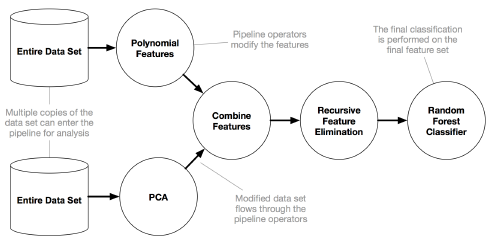
\includegraphics[scale=1]{MachineLearningPipeline.png}
		\caption{An example of a machine learning pipeline in \textit{TPOT}. It only shows the primitive algorithms and not hyper parameter terminals. At the root is the machine learning algorithm \cite{Gijsbers2017Thesis}.}
		\label{fig:MachineLearningPipeline}
	\end{figure}
	
	\begin{table}[]
		\centering
		\caption{All \textit{TPOT} Algorithms used for the \textit{TPOT} classifier function, their \textit{scikit-learn} class name is given. Not only the algorithms differ, but also the hyper-parameters within these algorithms.}
		\label{tab:TPOTAlgorithms}
		\begin{tabular}{ll|l}
			\textbf{Algorithm type} & \textbf{Specification}  & \textbf{Algorithms}                                                                                                        \\ \hline
			\multirow{5}*{\textbf{Classifier}}     & Naive Bayes             & GaussianNB, BernoulliNB, MultinomialNB                                                                                     \\ \cline{3-3}
			              & Decision Tree           & \begin{tabular}[c]{@{}l@{}}DecisionTree, ExtraTrees, RandomForest, \\ GradientBoosting\end{tabular}                        \\ \cline{3-3}
			              & Nearest Neighbour        & KNeighbours                                                                                                                 \\ \cline{3-3}
			               & Support Vector Machines & LinearSVC                                                                                                                  \\ \cline{3-3}
			               & LogisticRegression     & Logistic Regression                                                                                                        \\ \hline
			\multirow{4}*{\textbf{Preprocessors}} & Scaler                  & \begin{tabular}[c]{@{}l@{}}Binarizer, MaxAbsScaler, MinMaxScaler, \\ Normalizer, RobustScaler, StandardScaler\end{tabular} \\ \cline{3-3}
			               & Feature reduction       & \begin{tabular}[c]{@{}l@{}}PCA, FastICA, RBFSampler, Nystroem,\\  FeatureAgglomeration\end{tabular}                         \\ \cline{3-3}
			               & Feature Modifier        & Polynomial, OneHotEncoder,ZeroCount                                                                                        \\ \cline{3-3}
			              & Feature Selectors       & \begin{tabular}[c]{@{}l@{}}SelectFwe, SelectPercentile, VarianceThreshold, \\ RFE, SelectFromModel\end{tabular}   
		\end{tabular}
	\end{table}
	
	% TPOT mutation operators
	\textit{TPOT} has three different types of mutations within one pipeline. The first one is insertion, inserting a primitive somewhere in the tree. An example would be the insertion of an additional preprocessing algorithm. The second one is replacement, which replaces a random terminal. It can for example change a binary hyper parameter from true to false. The third one is shrinking. A primitive is replaced by a terminal. For example a preprocessing step can be replaced by just raw data. This different mutations can all be seen visually (Figure \ref{fig:TPOTMutations})
	
	\begin{figure}[h!]
		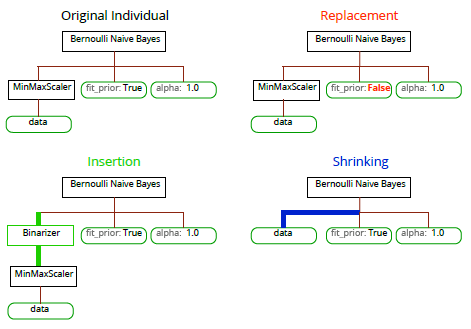
\includegraphics[scale=1]{TPOTMutations.png}
		\caption{Examples of the three mutations in the \textit{TPOT} algorithm: insertion, replacement and shrinking \cite{Gijsbers2017Thesis}.}
		\label{fig:TPOTMutations}
	\end{figure}
	
	% Crossover
	TPOT also focuses on mutations between two pipelines by means of crossovers. Between two pipelines, sub-trees and primitives can be changed, given that the both pipelines remain valid (Figure \ref{fig:TPOTCrossover}). Every time a crossover is performed, two separate pipelines are used and changed, creating two new ones.
	
	\begin{figure}[h!]
		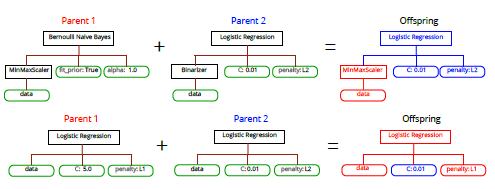
\includegraphics[scale=1]{TPOTCrossover.png}
		\caption{An example of a \textit{TPOT} crossover \cite{Gijsbers2017Thesis}.}
		\label{fig:TPOTCrossover}
	\end{figure}
	
	% Biomedical preprocessing
	Considering the capabilities from \textit{TPOT} to cope with challenges in biomedical data, several methods are available. It has several different normalisation/standardisation scalers (StandardScaler, RobustScaler, MinMaxScaler) to tackle feature heterogeneity between different data sets and errors. It also has some feature selection operators to tackle errors (VarianceThreshold, SelectKBest, SelectPercentile). Wrapper methods however are not included, which may perform better in some situations. At last, if missing values are present, it imputes the median for those values before starting the evolutionary algorithm. However, it does not have any possibilities to handle non-numeric data. If non-numeric data is present, the user first needs to preprocess himself.
	
	% Disadvantage
	A big variety of algorithms are present for TPOT, as well as numerous hyper parameter values for those algorithms. This is both an advantage as an disadvantage as probably most algorithms and hyper parameter combinations are not useful as an outcome. Since TPOT randomly chooses mutations, possibly better algorithms could be chosen with less random choices. For example meta-features could be used to improve the algorithm selection.
	
	\newpage
	\section{Hypotheses}
	\label{FSsec:hypotheses}
	
	The main goal of this chapter is to find more insight in feature selection and add that insight to the final framework. Several hypotheses are made before designing experiments to test them and they are discussed here:
	
	\begin{enumerate}
		\item \textit{Optimum in number of selected features} \\
		An optimum should be found in the selected features. Whereas using too many features may cause issues for a machine learning algorithms to extract the correct information from them, preserving too few features may result in lost information. Previous research scaled down the number of features from 400 to 96 \cite{pazzani1997learning}, 500 to 13 and for even bigger datasets from 5000-100000 features to between 200 and 900 relevant features \cite{chen2006combining}. Interestingly, the number of relevant features was not related to the original feature set size, indicating the optimum to be an absolute number. Therefore: \\
		\\
		\emph{H1: The value of this absolute optimum is estimated to be lower than 1000, as no study before ever used a higher number of relevant features.}\\
		\\
		\item \textit{Best feature selection methods} \\
		Three types of feature selection methods are discussed, all of them having their own advantages. Out of these three, the embedded methods are expected to outperform the others. Whereas filter methods are quick and easy, their efficiency should be lower than the other methods. Wrapper methods are closer to trying to find the optimal solution in an exhaustive search way. Therefore they are expected to perform best in feature selection at the cost of computation efficiency. At last the embedded methods are expected to be in between of the two. The embedded methods use machine learning methods that are fairly quick and easy to understand. Those machine learning methods also use relative contributions between features. This would mean that embedded methods are quicker and easier than wrapper methods and more efficient than filter methods and therefore combining the best of both. \\
		\\
		\emph{H2: The embedded methods are expected to outperform filter methods in quality and wrapper methods in computation time efficiency.}\\
		\\
		\item \textit{TPOT feature selection integration} \\
		Integration of feature selection in \textit{TPOT} for the framework can be done in different ways. Two ways are thought to be a beneficial addition to the tool. First expanding the number of feature selection methods should improve \textit{TPOT} in finding better pipelines. Secondly having \textit{TPOT} start with an initial pool of pipelines including feature selection methods should give it a head-start and therefore be quicker and better and finding good pipelines.\\
		\\
		\emph{H3: Both additions (warm starting with feature selection methods and additional feature selection methods) are expected to improve \textit{TPOT} with feature selection.}\\
		\\
		
				
	\end{enumerate}
	
	\newpage
	\section{Methods}
	\label{FSsec:Methods}
	
	% Introduction methods
	For empirical evaluation the collection of feature selection methods experiments are done. The quality of the feature selection is tested by defining a definition of quality first. After that an exploration of feature selection is done with filter methods, followed by comparisons of multiple feature selection methods. The four example datasets (subsection \ref{DEsubsec:Datasets}) were used as example datasets for the experiments.
	
	\subsection{Feature Selection Quality}
	\label{FSsubsec:DimensionalityReductionQuality}
	
	% Machine learning for testing
	To find out the quality of the feature selection, multiple machine learning algorithms are used \cite{hall1998practical}.  Classification of the datasets can be done with several machine learning algorithms and validation and tests scores show how well the data can be classified after feature selection. The quality will be described with the accuracy of machine learning algorithms: the number of right classifications divided by the total number of classifications. Five different machine learning classifiers are used from \textit{scikit-learn}: logistic regression, decision trees, nearest neighbour, support vector machines and Naive Bayes. Better feature selection algorithms have relatively higher accuracy, as they are better at preserving the right features. Since over fitting sometimes happens when fitting data in a machine learning algorithm, both a validation and a test score is computed for the accuracy. For every experiment a training set and a test set is created, making the test set 20\% of the complete dataset. A validation score is computed by using the "leave one out" technique on the training set and a test score is computed by testing the classification score of the test set. Since the samples are not evenly distributed over the classes the precision, recall and F1 scores are also computed to find potential bias in the result.
	
	% Addition to number of features
	In some cases the quality of the machine learning algorithm lacks a factor of feature subset size. The standard score in those cases is not sufficient enough to evaluate the result. To incorporate the quality of feature selection a new modified quality term \textit{FS\_score} is created (Equation \ref{eq:FSAccuracy}). In \textit{FS\_score} a modified version of the original score, in this thesis being accuracy, is given by first multiplying it by a factor dependent on the number of features. This factor consists of a constant $\beta$, a value in range $[0, 1]$ which can be chosen for the influence of the  value that represent the number of features. In practice $\beta > 0.95$ so the reduction does not have too much influence on the score. An example plot of how the correction factor changes is given (Figure \ref{fig:FSAccuracyPlot}).
	
	\begin{equation*}
	\label{eq:FSAccuracy}
	\text{FS\_score} = \text{score} \times \beta^{\text{\#features}}
	\end{equation*}
	
	% Insert figures
	\begin{figure}[H]
		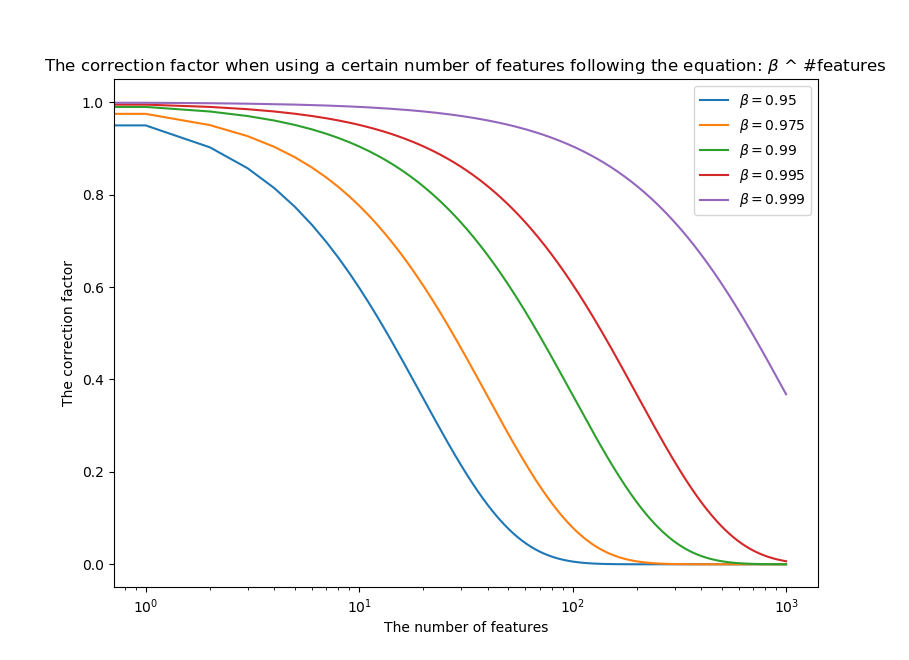
\includegraphics[width=1\textwidth]{FS_accuracy_alpha.png}
		\caption{The correction factor for the \textit{FS\_score} from Equation \ref{eq:FSAccuracy}. Every graph corresponds to a different value of $\beta$.}
		\label{fig:FSAccuracyPlot}
	\end{figure}
	
	% Absolute number of features
	The factor \mbox{\#features} is an absolute count, instead of a relative count (for example a percentage of features). The reason for using an absolute count can be found in the goal of the data analysis. In data analysis the number of features that can be relevant are very limited. Useful results need relations between the input and the output, and these relations need to be as simple as possible. If the number of features is relative to the total number of features, the input size can change significantly. Take for example the Micro-organisms and the RSCTC datasets provided for this study (Subsection \ref{DEsubsec:Datasets}). 2\% of the total features would be 26 and 1100 features for these datasets respectively. Whereas relations between 26 features and the output is possible to understand, relations between 1100 features and the output is much harder. Taking an absolute number of features allows for a more active choice on the input size.
	
	% Selection proper beta
	To put the impact of the \textit{FS\_score} in perspective, an example figure is made how the outcome is computed (Figure \ref{fig:FSAccuracyExample}). This figure shows the impact on the performance of a method when using a certain number of features. After using a correction factor, an optimum is created for which the number of features is important, the old optimal score did not include the number of features. The example (with $\beta = 0.99$) seems to give a good indication of the desired outcome. For every $10$ features, the \textit{FS\_score} is reduced by about 10\% (Figure \ref{fig:FSAccuracyPlot}), which meant for the example filter method that for 50 features an optimum was reached (Figure \ref{fig:FSAccuracyExample}). Because of this empirically found desired trade-off, $\beta = 0.99$ will be chosen in this project when using \textit{FS\_score}. 
	
	% Insert figures
	\begin{figure}[H]
		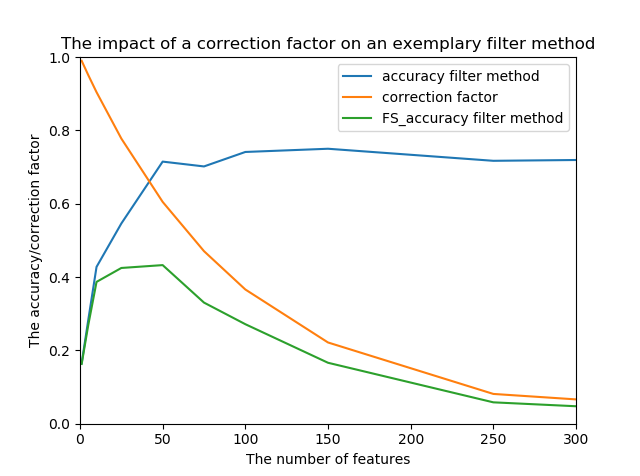
\includegraphics[]{FS_accuracy_example.png}
		\caption{An example of the impact of the correction factor on the score, in this case accuracy. The shown correction factor uses $\beta = 0.99$. On the x-axis the number of features is shown and on the y-axis the value for the original accuracy, the correction factor and the \textit{FS\_score}.}
		\label{fig:FSAccuracyExample}
	\end{figure}
	
	\subsection{Feature Selection Exploration}
	\label{FSsubsec:FeatureSelectionExploration}
	
	% First experiment
	The first set of experiments is used to explore a combination of the basic filter method combined with the quality measurements. The basic filter method algorithm selecting the top $n$ features (Algorithm \ref{alg:FilterTopNAlgorithm}) is used. The changing variables are the dataset, the ranking method, the feature preservation values and the accuracy computation methods (Table \ref{tab:FirstExperimentRequirements}). The range of chosen feature preservation values comes from both its ability to show impact of separate features (more impact from fewer features) and the relevance of keeping that number of features (irrelevant feature selection when having more than 1000 features). All of this together results in a total of $4 (\text{datasets}) \times 2 (\text{ranking methods}) \times 11 (\text{top } n \text{ features}) \times 5 (\text{accuracy computation methods}) = 440$ experiments. These experiments are visualized in eight plots, one plot for every combination of data set and ranking method. These plots then show the change in quality for different number of preserved features.
	
	\begin{table}[]
		\centering
		\caption{The four meta-parameters with their possible values in the first experiment.}
		\label{tab:FirstExperimentRequirements}
		\begin{tabular}{l|ll}
			\textbf{Variable} & \textbf{Description}                                                                              & \textbf{Values}                                                                                                                         \\ \hline
			Dataset           & The datasets used (subsection \ref{FSsubsec:Datasets})                                                                                 & \begin{tabular}[c]{@{}l@{}}Psoriasis\\ RSCTC\\ Arcene\\ Micro-Organisms\\ --\end{tabular}                                               \\
			Ranking method    & \begin{tabular}[c]{@{}l@{}}The method used for ranking \\ the features (
				Subsection \ref{FSsubsec:FilterMethods})\end{tabular}               & \begin{tabular}[c]{@{}l@{}}T-test (\textit{SciPy})\\ Mutual Information (\textit{scikit-learn})\\ --\end{tabular}                                                                \\
			Feature preservation values & \begin{tabular}[c]{@{}l@{}}The fixed size of the feature subset \\ after feature selection\end{tabular} & \begin{tabular}[c]{@{}l@{}}1, 5, 10, 25, 50, 75, \\ 100, 150, 250, 500, 1000\\ --\end{tabular}                                          \\
			Accuracy computation & \begin{tabular}[c]{@{}l@{}}The machine learning algorithms \\ used to compute accuracy (subsection \ref{FSsubsec:DimensionalityReductionQuality})\end{tabular}   & \begin{tabular}[c]{@{}l@{}}Naive Bayes\\ Logistic Regression\\ Support Vector Machine\\ Decision Tree\\ Nearest Neighbours\end{tabular}
		\end{tabular}
	\end{table}
	
	\subsection{Feature Selection Algorithms Evaluation}
	\label{FSsubsec:FeatureSelectionAlgorithmsEvaluation}
	
	% Second experiment
	The second set of experiments compares the feature selection methods in both feature selection and quality. For this experiment the four datasets are used with the logistic regression quality measurement, since the logistic regression gave the most consistent result of the five machine learning algorithms, showing the smallest variation across the datasets. The average performance for all datasets is also computed for clarification purposes. An overview of feature selection methods is made (Table \ref{tab:SecondExperimentMethods}) and all separate meta-parameters are explained here.
	
	\begin{itemize}
		\item \textit{Filter methods} \\
		The ranking methods T-test and Mutual Information were used as those were both explored in the first experiment. The thresholds of 50, 100 and 150 features were chosen as a compromise between the desired number of features (as few as possible) and the quality of the result (as explored in the first experiment).
		\item \textit{Wrapper methods} \\
		The order of the features used for feature selection with wrapper methods was put at random (no special ordering) or with mutual information (special ordering). The evaluation was chosen to be Naive Bayes as it is simple and not much affected by conditional dependency. The aforementioned threshold value for wrapper methods $\alpha$ was chosen to be 0.01 and 0.001 with a maximum number of features in mind. If $\alpha= 0.01$, a feature will only be added when it raises the quality by 0.01. The accuracy can be at most 1, so at most 100 features can be added, even though the final number of features would be much less. $\alpha = 0.001$ was taken for a solution with a higher accuracy in mind. At last, for the PTA method, for $l$ and $r$ the combinations $[l, r] = [5, 2]$ and $[l, r] = [20, 10]$ were chosen. The ratio was picked close to $2:1$ as a compromise between number of features added and removed, 50\% being a reasonable ratio to still keep a decent number of features. The size of $l$ and $r$ were different in a factor $4$ or $5$ to find out if this size difference would make a change.
		\item \textit{Embedded methods} \\
		The machine learning algorithms that were tested were Support Vector Machines (SVM) and RandomForests (rf), as both of them have a measurement of feature importance. The number of features preserved was put on 50, 100 and 150 being the same as for the filter methods.
		
		
	\end{itemize}
	Spectra are made with the results of the experiment that show the performance of all different combinations, showing the accuracy, precision, recall and F1-score. On top of that the computation time is computed and shown per algorithm, as well, in a separate bar chart. At last a combination of the earlier proposed \textit{FS\_score} and the computation time is shown as well for $\alpha = 0.99$ to show the relation between computation time on one hand and the \textit{FS\_score} on the other hand. 
	Several discussed algorithms  are chosen to be excluded from the evaluation. This choice is based on their poor scalability with regards to computation time and therefore unfit for datasets with this many features. These excluded algorithms are the backwards elimination sequential method, the simulated annealing stochastic search method and the embedded backwards elimination method (Subsection \ref{FSsubsec:FeatureSelectionMethods}). 
	
	\begin{table}[]
		\centering
		\caption{The methods that are evaluated in the second experiment setup.}
		\label{tab:SecondExperimentMethods}
		\begin{tabular}{l|ll}
			\textbf{Type}                    & \textbf{Method}                                                             & \textbf{Parameters}                                                                                                                                                                          \\ \hline
			Filter methods                   & \begin{tabular}[c]{@{}l@{}}Basic Filter Methods\\ (Algorithm \ref{alg:FilterTopNAlgorithm})\end{tabular} & \begin{tabular}[c]{@{}l@{}}- Rank: T-test, Mutual Information\\ - Thresholds: 50, 100, 150 features\end{tabular}                                                                             \\ \hline
			\multirow{3}{*}{Wrapper methods} & \begin{tabular}[c]{@{}l@{}}Forward selection\\ (Algorithm \ref{alg:ForwardSelection})\end{tabular}    & \begin{tabular}[c]{@{}l@{}}- Order: Random, Mutual Information\\ - Evaluation: Naive Bayes\\ - Alpha: 0.01, 0.001\\ --\end{tabular}                                             \\
			& \begin{tabular}[c]{@{}l@{}}PTA\\ (Algorithm \ref{alg:PTA})\end{tabular}                  & \begin{tabular}[c]{@{}l@{}}- Order: Random, Mutual Information\\ - Evaluation: Naive Bayes\\ - {[}l, r{]} = {[}20, 10{]}, {[}5, 2{]}\\ - Alpha: 0.01, 0.001\\ --\end{tabular} \\
			& \begin{tabular}[c]{@{}l@{}}Floating search\\ (Algorithm \ref{alg:FloatingSearch})\end{tabular}      & \begin{tabular}[c]{@{}l@{}}- Order: Random, Mutual Information\\ - Evaluation: Naive Bayes\\ - Alpha: 0.01, 0.001\end{tabular}                                                                                 \\ \hline 
			Embedded methods                 & \begin{tabular}[c]{@{}l@{}}Forward selection\\ (Algorithm \ref{alg:EmbeddedForwardSelectionAlgorithm})\end{tabular}    & \begin{tabular}[c]{@{}l@{}}- Machine Learning: SVM, RandomForests\\ - Threshold: 50, 100, 150 features\end{tabular}                                                                         
		\end{tabular}
	\end{table}
	
	\subsection{TPOT Feature selection integration}
	\label{FSsubsec:TPOTEvaluationIntegration}
	
	% Introduction
	TPOT is an effective tool to find the best machine learning pipeline for a certain dataset (Subsection \ref{FSsubsec:AutomatedMachineLearning}). \textit{TPOT} however has three restrictions on finding the correct pipeline when a high number of features is involved:
	
	\begin{enumerate}
		\item \textit{Input versus output} \\
		The goal of feature selection is to directly link a smaller number of features to the output. Whereas \textit{TPOT} has possibilities to find pipelines with feature selection, it gives no advantage to pipelines that actively use feature selection if needed.
		\item \textit{Memory/Invalid dataset issues} \\
		Firstly, not all algorithms are suitable for handling more than 10000 features. The feature agglomeration algorithm, one of the algorithms present in \textit{TPOT}, will create memory issues in those cases. This makes this algorithm unfit for usage. Similarly, the \textit{scikit-learn} multinomial Naive Bayes algorithm cannot be used with negative values. Biomedical data does not have that restriction and therefore possibly gives errors because of this. On top of that, several preprocessing algorithms also change values to be negative.
		\item \textit{General insert issue} \\
		After some testing and consultation it was concluded that inserting new algorithms to a pipeline created issues in \textit{TPOT}.  These issues resulted in a very low number of insertion mutations, which caused a suboptimal search for the best machine learning pipeline that includes feature selection methods and insertion of those.
	\end{enumerate}
	
	% Sulotion to this three restrictions
	These three initial restrictions must first be tackled for proper use of \textit{TPOT} with feature selection. This resulted in three measures, explained here in corresponding order.
	
	\begin{enumerate}
		\item \textit{Feature modifier addition to accuracy} \\
		In the case of feature selection, the possibility is given to change the performance measurement to the earlier proposed \textit{FS\_score}. Using this \textit{FS\_score} instead of normal accuracy creates an incentive for \textit{TPOT} to prefer feature selection algorithms in the resulting pipeline, due to higher performance.
		\item \textit{Algorithm removal} \\
		For this restriction, simply the feature agglomeration algorithm is removed. This type of feature selection is not essential in biomedical research and therefore removal is not expected to hinder removal. The multinomial Naive Bayes algorithm is removed, as well, with the same reasoning.
		\item \textit{Change in insert method} \\
		This insert issue was removed by rewriting the code for the insert function. This insert function originally attempted to insert algorithms for every possible hyper-parameter as well as at the start of the pipeline. This is replaced by only having insertion at the start of the pipeline This is an improvement because no algorithm in \textit{TPOT} actually has a hyper-parameter that can be changed by a different algorithm in \textit{TPOT}.
	\end{enumerate}
	
	On top of these three restrictions and the measures taken to tackle them, two additional restrictions hinder optimization regarding feature selection:
	
	\begin{enumerate}
		\item \textit{Lack of warm start} \\
		TPOT has a vast array of machine learning and preprocessing algorithms to find the best possible pipeline. Due to the number of possibilities being very high, a lot of time may be wasted due to searching in wrong directions. For feature selection, a pre-defined selection of pipelines (also known as a warm start) would improve efficiency.
		\item \textit{Feature selection possibilities} \\
		Several filter and embedded methods are present (Subsection \ref{FSsubsec:FeatureSelectionMethods}). All of these select percentages of feature selection, though. Still a high number of features can be present in the result after using percentages. On top of that, no wrapper methods are available, either.
	\end{enumerate}
	
	For both of these optimization restrictions, two additions are made to the \textit{TPOT} code structure for increased functionality with regards to feature selection, in the same order as the restrictions:
	
	\begin{enumerate}
		\item \textit{Focused feature selection addition} \\
		The possibility is created to always start the original population with a feature selection algorithm in the feature selection pipeline. Due to this start the expected search for a good feature selection method is bypassed immediately, which should result in more optimized final pipeline.
		\item \textit{Alternative feature selection algorithm set} \\
		The possibility is created to start with an alternative feature selection algorithms set. This selection consists of filter, wrapper and embedded methods and the hyper-parameters are predefined to create an upper bound of 200 features.
	\end{enumerate}
	
	% Outcome explanations
	The outcome of the first initial measures are trivial: the use of \textit{FS\_score} makes \textit{TPOT} search for solutions with fewer features. The removal of algorithms that cause errors and memory issues creates better optimization. Furthermore more effective use of the insert evolution, makes the algorithm make better use of that possibility. The outcome of optimization additions however may not necessarily improve the performance of \textit{TPOT} for feature selection. Therefore the changes for these two solutions are tested with an experiment. 
	
	% Experiment set-up
	The experiment consists of multiple runs of \textit{TPOT} and all of these steps are also shown in an explanatory table (Table \ref{tab:TPOTExpDetails}). All four datasets are tested (Subsection \ref{FSsubsec:Datasets}) and the accuracy is changed to the feature sensitive \textit{FS\_score} with $\beta = 0.99$ (Equation \ref{eq:FSAccuracy}), as previously discussed (Subsection \ref{FSsubsec:DimensionalityReductionQuality}). For testing \textit{TPOT} an optimization time of 120 minutes (two hours) was chosen as a reasonable time constraint to run each experiment 5 times, an algorithm was not allowed to run for longer than ten minutes, a population size of 12 was chosen to not be to selective at the start and a training set size of $0.90$ which is a general training set size when not many samples are present. Furthermore tests were done for pipeline selection both with and without focused feature selection  and for both with and without alternative feature selection algorithms set, as these additions must be tested for their quality. This gives a total of $4 (\text{datasets}) \times 2 (\text{pipeline selection}) \times 2 (\text{feature selection set}) \times 5 (\text{experiment reruns}) = 16$ different experiments.
	
	
	\begin{table}[]
		\caption{The experiment details for testing the non-trivial changes in \textit{TPOT}. This experiment is rerun 5 times.}
		\label{tab:TPOTExpDetails}
		\begin{tabular}{l|l|l}
			\textbf{\begin{tabular}[c]{@{}l@{}}Experiment \\ factors\end{tabular}}                           & \textbf{Detailed values}                                                                                                                                                                    & \textbf{Remarks}                                                                                                                                                                                                                                    \\ \hline
			\textbf{Datasets}                                                                                & \begin{tabular}[c]{@{}l@{}}Micro-organisms\\ Arcene\\ RSCTC\\ Psoriasis\end{tabular}                                                                                                         & \begin{tabular}[c]{@{}l@{}}High number of features\\ (Subsection \ref{FSsubsec:Datasets})\end{tabular}                                                                                                                                                                  \\ \hline
			\textbf{\begin{tabular}[c]{@{}l@{}}Performance \\ measurement\end{tabular}}                      & \begin{tabular}[c]{@{}l@{}}One type: \textit{FS\_score}\\ - $\beta = 0.99$\end{tabular}                                                                                                             & \begin{tabular}[c]{@{}l@{}}Addition of correction factor\\ (Equation \ref{eq:FSAccuracy})\end{tabular}                                                                                                                                                              \\ \hline
			\textbf{\begin{tabular}[c]{@{}l@{}}TPOT input \\ parameters\end{tabular}}                        & \begin{tabular}[c]{@{}l@{}}One set of input values:\\ - max. optimization time = 120 min\\ - max. alg. evaluation time = 10 min\\ - pop. size = 12 \\ - train size = 0.9\end{tabular} & \begin{tabular}[c]{@{}l@{}}Explanation of input values:\\ - The time one run should take (2 hours)\\ - The evaluation time of one pipeline \\ - The number of pipelines in one generation\\ - The number of samples used for training\end{tabular} \\ \hline
			\textbf{\begin{tabular}[c]{@{}l@{}}Pipeline\\ selection\end{tabular}}                           & \begin{tabular}[c]{@{}l@{}}Regular selection\\ Feature selection focused\end{tabular}                                                                                                       & \begin{tabular}[c]{@{}l@{}}Possible obligatory addition \\ of a feature selection algorithm\end{tabular}                                                                                                                                            \\ \hline
			\textbf{\begin{tabular}[c]{@{}l@{}}Change in \\ feature selection \\ algorithm set\end{tabular}} & \begin{tabular}[c]{@{}l@{}}Regular feature selection algorithm set\\ New feature selection algorithm set\end{tabular}                                                                       & \begin{tabular}[c]{@{}l@{}}A change between several basic \\ feature selection algorithms to \\ feature selection algorithms designed \\ for at most 200 features preservation\end{tabular}                                                        
		\end{tabular}
	\end{table}
	
	\newpage
	\section{Results}
	\label{FSsec:Results}
	
	The different experiments are all explained in their own subsections. First the results of the minimum feature preservation experiment were shown, followed by the feature selection algorithms evaluation.
	
	\subsection{Feature Selection Exploration Results}
	\label{FSsubsec:FeatureReductionExplorationResults}
	
	The results were plotted for every dataset separately (Appendix \ref{app:FeatureSelectionExplorationPlots}). An average of the four datasets was also created to show the difference between validation and test score (Figure \ref{fig:ValTestScores}), between machine learning quality measures (Figure \ref{fig:MachineLearningQualityScores}) and between data sets with ranking methods (Figure \ref{fig:DatasetRankScores}).
	
	% Insert figures
	\begin{figure}[H]
		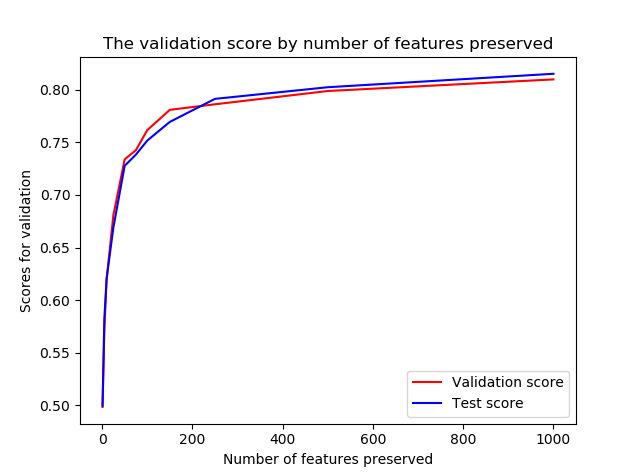
\includegraphics[width=0.7\textwidth]{Val_Test_Scores.png}
		\caption{The average validation and test scores after averaging the scores for the data sets and ranking methods.}
		\label{fig:ValTestScores}
	\end{figure}
	
	% Discussion result validation and test scores
	As could be seen (Figure \ref{fig:ValTestScores}) the difference between the validation and the test scores was very low. The average almost showed two identical curves which indicates that there was hardly any over fitting present for filter methods. The test error should not be higher than the validation error usually, but in this case the test error had a higher variance. The test error was only one measurement (after splitting the data into training and test set) and the validation error was found with leave-one-out, which should have a much lower variance. Because of the lower variance, the validation score was used in the other two figures (Figures \ref{fig:MachineLearningQualityScores} and \ref{fig:DatasetRankScores}).
	
	% Insert figures
	\begin{figure}[H]
		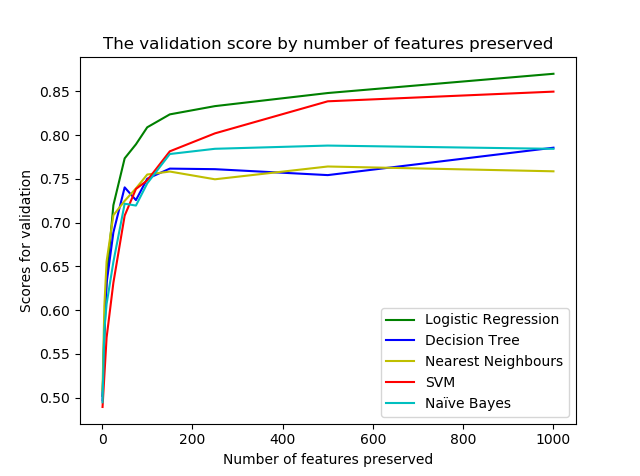
\includegraphics[width=0.7\textwidth]{Machine_Learning_Val_Scores.png}
		\caption{The average validation accuracy shown per machine learning quality measurement.}
		\label{fig:MachineLearningQualityScores}
	\end{figure}
	
	% Discussion machine learning quality scores
	Logistic regression gave the best validation scores taking all data sets combined, followed by SVM. Also, when looking at all eight plots separately (Appendix \ref{app:FeatureSelectionExplorationPlots}), logistic regression also showed the most consistent behaviour. All five of the machine learning algorithms showed an 'elbow', an area in the graph for which the score stops growing as much when more features are used. This 'elbow' was located around 100 features with 200 features being the end for almost every 'elbow'.
	
	% Insert figures
	\begin{figure}[H]
		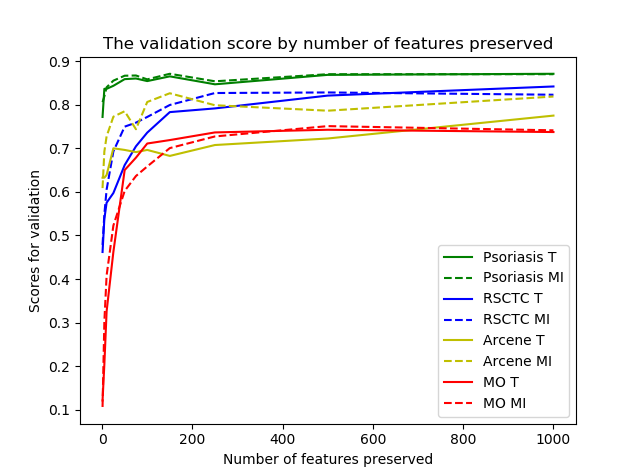
\includegraphics[width=0.7\textwidth]{Data_Rank_Val_Scores.png}
		\caption{The average validation accuracy shown per dataset and rank.}
		\label{fig:DatasetRankScores}
	\end{figure}
	
	% Discussion machine learning quality scores
	A difference in score quality for the datasets was visible (Figure \ref{fig:DatasetRankScores}). The difference between using Mutual Information and T-test/ANOVA was not, as for only the Arcene dataset there was a significant difference between the two. Therefore it seems that the ranking method type has less influence on the measurement quality. One interesting aspect was that methods using Mutual Information had a longer computation time than methods using the T-test/ANOVA.
	
	% Precision/Recall/F1
	Accuracy was used to test the validation quality of the filter methods. Aside from accuracy the precision, recall and F1-score were also computed to find out whether accuracy is a proper representation of the quality (Figures \ref{fig:DatasetRankScores} and \ref{fig:DatasetRankF1Scores} and Appendix \ref{app:PrecisionRecall}). These scores showed that the accuracy is a plausible way to depict quality and it is not needed to use F1-score. Only the Arcene dataset shows some difference between accuracy, precision, recall and the F1-score but these differences would not affect any conclusions.
	
	% Insert figures
	\begin{figure}[H]
		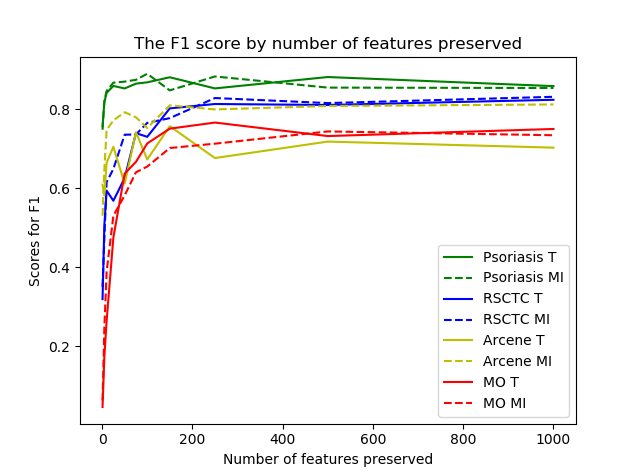
\includegraphics[width=0.7\textwidth]{Data_Rank_F1_Scores.png}
		\caption{The average validation F1-scores shown per dataset and rank.}
		\label{fig:DatasetRankF1Scores}
	\end{figure}
	
	\subsection{Feature Selection Algorithms Evaluation Results}
	\label{FSsubsec:FeatureSelectionAlgorithmsEvaluationResults}
	
	% Figures + first observations
	Spectra using all basic filter methods and wrapper sequential search methods were created, averaging the accuracy (Figure \ref{fig:Avg_Accuracy_Spectrum}), precision (Appendix \ref{app:EvaluationPlots}), recall (Appendix \ref{app:EvaluationPlots}) and F1 score (Figure \ref{fig:Avg_F1_Spectrum}) of the four datasets. The figures showed that all wrapper algorithms preserved on average less than 61 features for these settings, whereas the performance seems to average around 75\% for all four performance scores. The filter and embedded methods performed worse, with an overall lower performance score than the wrapper methods, even when more features were present. Also, no immediate observations can be made by looking only at the filter and embedded algorithms.
	
	% Wrapper algorithms observations
	When only looking at the wrapper algorithms, some other observations could be done, as well. Ordering the features before using a wrapper method structurally gave a better result than using a random ordering. Also a threshold of $\alpha = 0.001$ usually resulted in more features and in a higher scores in comparison with a threshold of $\alpha = 0.01$. Comparing the algorithms, the floating search with ordering did best in performance, whereas the other algorithms are performing closer together.
	
	% Insert figures
	\begin{figure}[H]
		\centering
		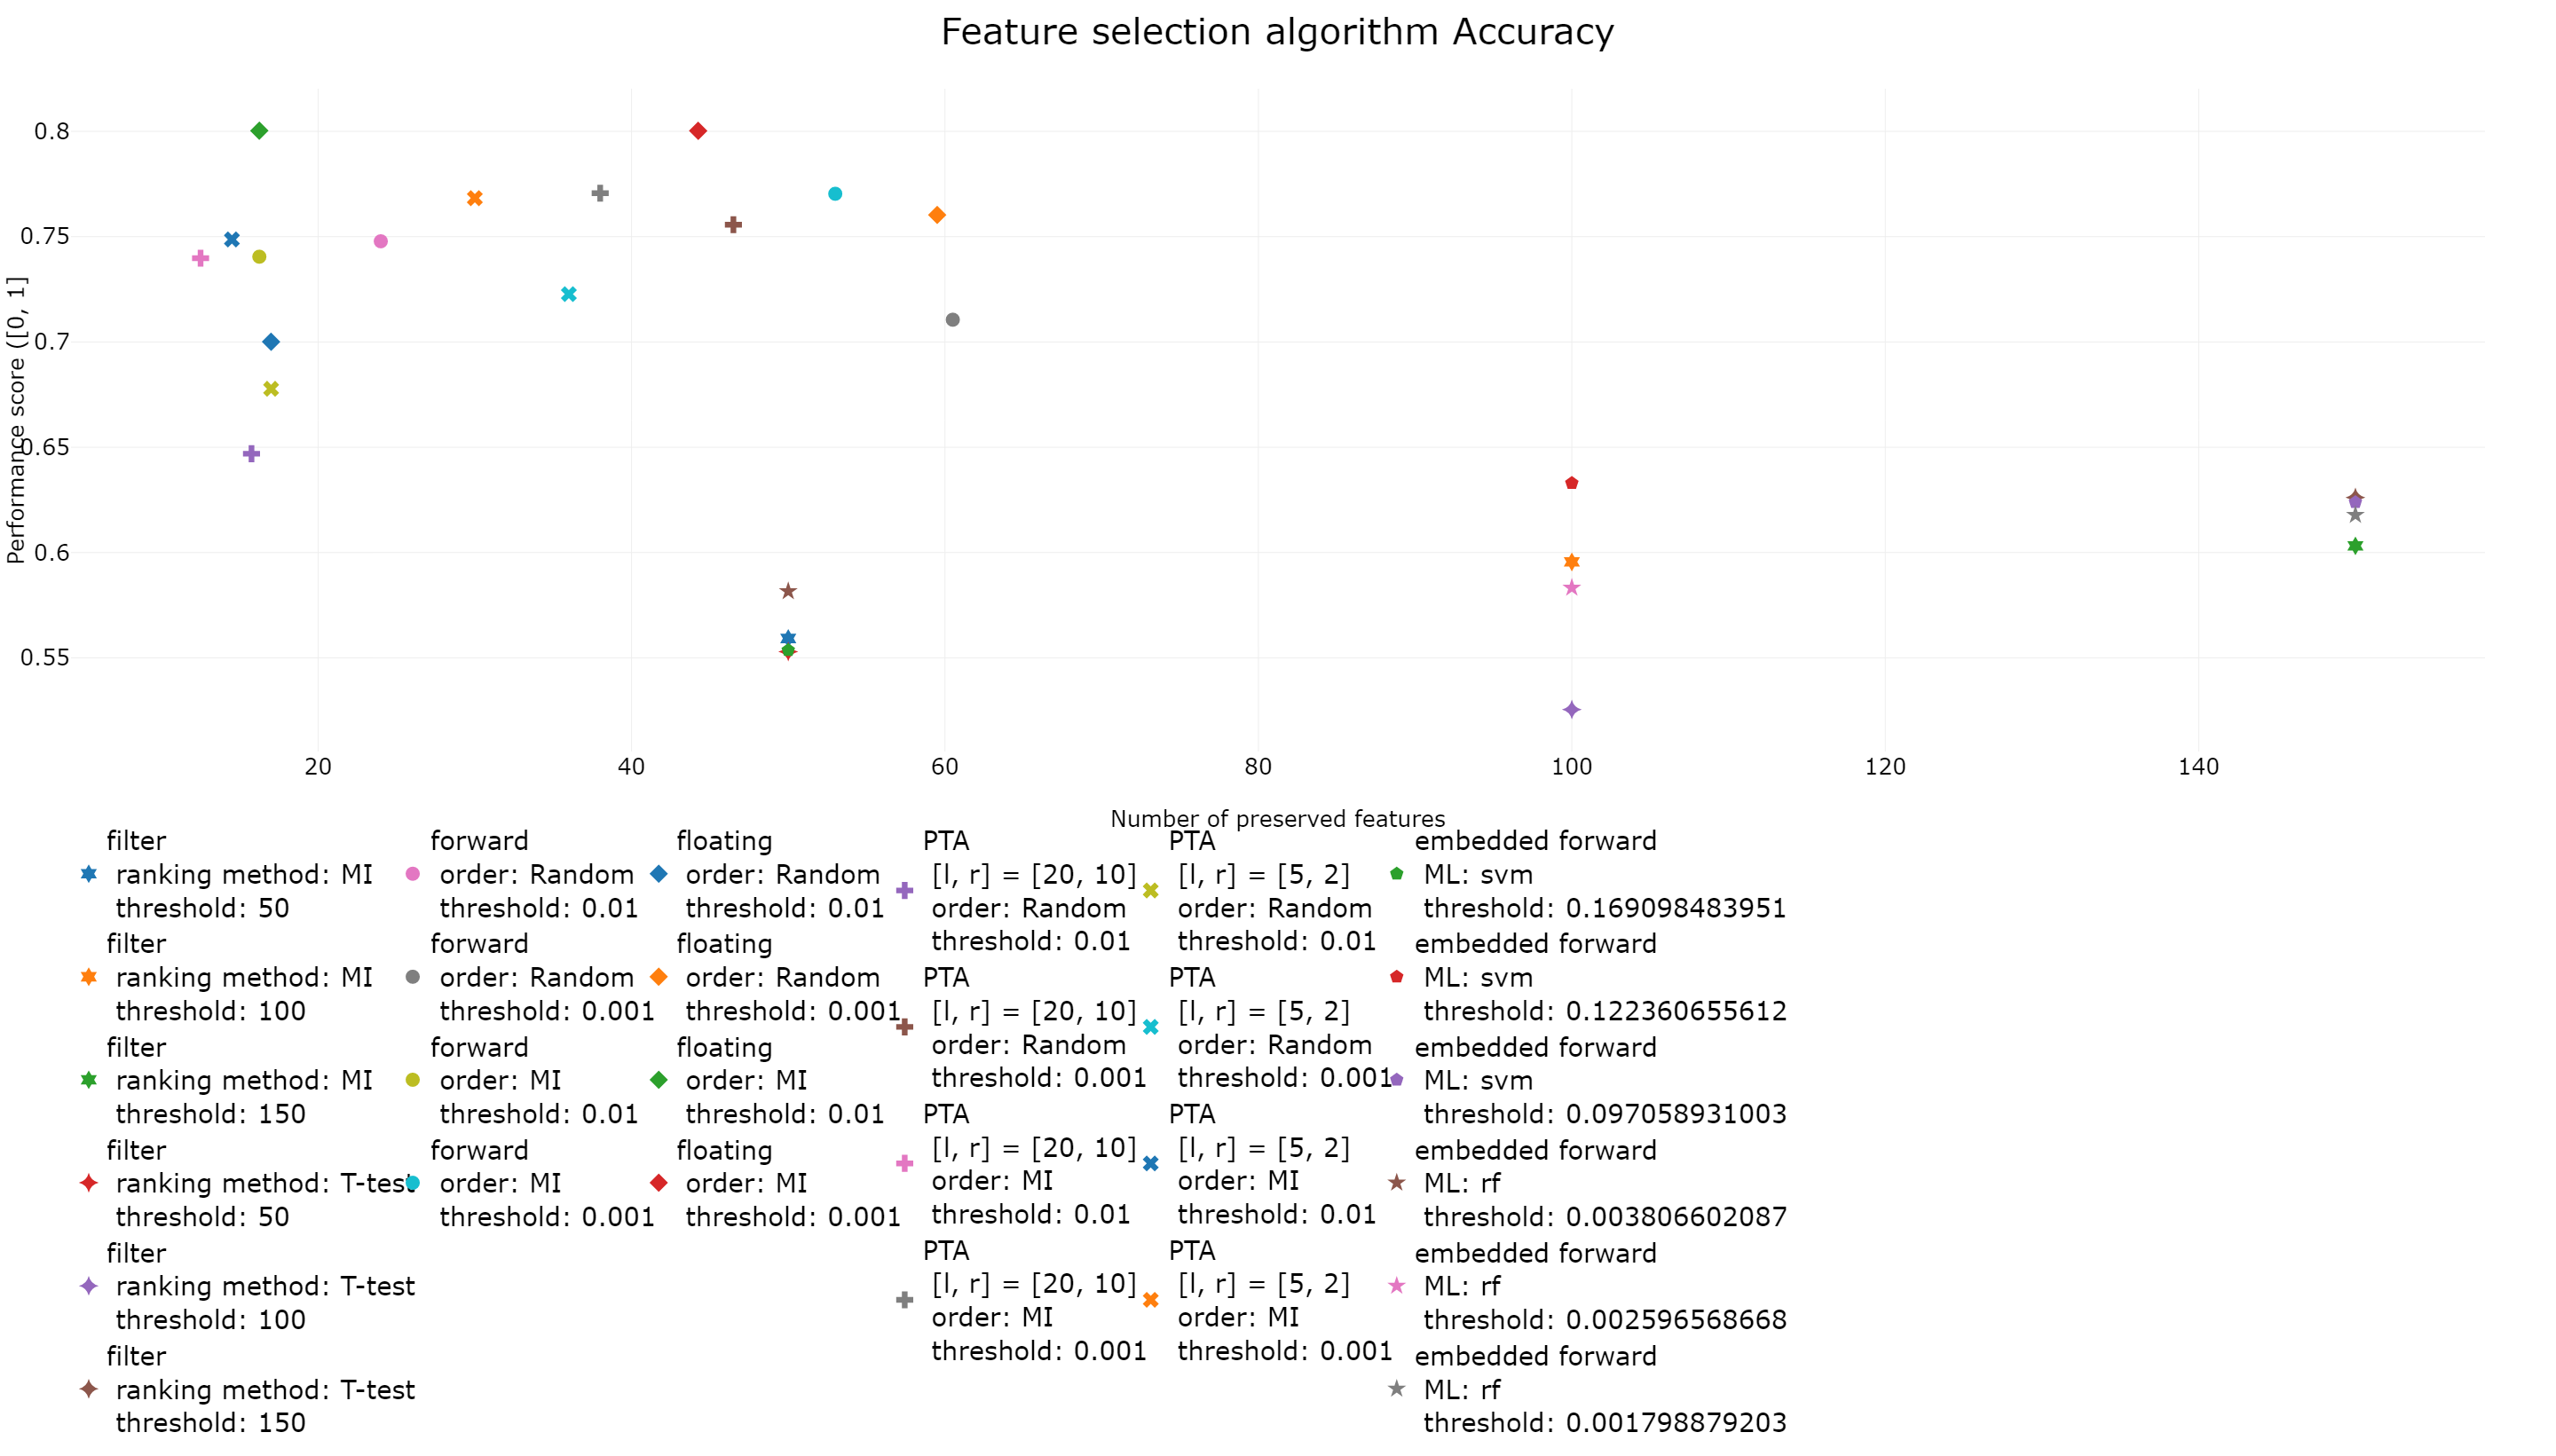
\includegraphics[angle=90,height=1.4\textwidth]{Accuracy_new.png}
		\caption{The accuracy spectrum for the average dataset. The x-axis shows the average number of features that are preserved and the y-axis shows the accuracy of logistic regression. The legend indicates the algorithms (Table \ref{tab:SecondExperimentMethods}) and their corresponding shapes, as well as the chosen parameters with their matching colours. Abbreviations in legend: Mutual Information (MI), Pick l-Take Away r (PTA), Machine Learning algorithm (ML), Support Vector Machine (svm), random forest (rf)}
		\label{fig:Avg_Accuracy_Spectrum}
	\end{figure}
	
	% Insert figures
	\begin{figure}[H]
		\centering
		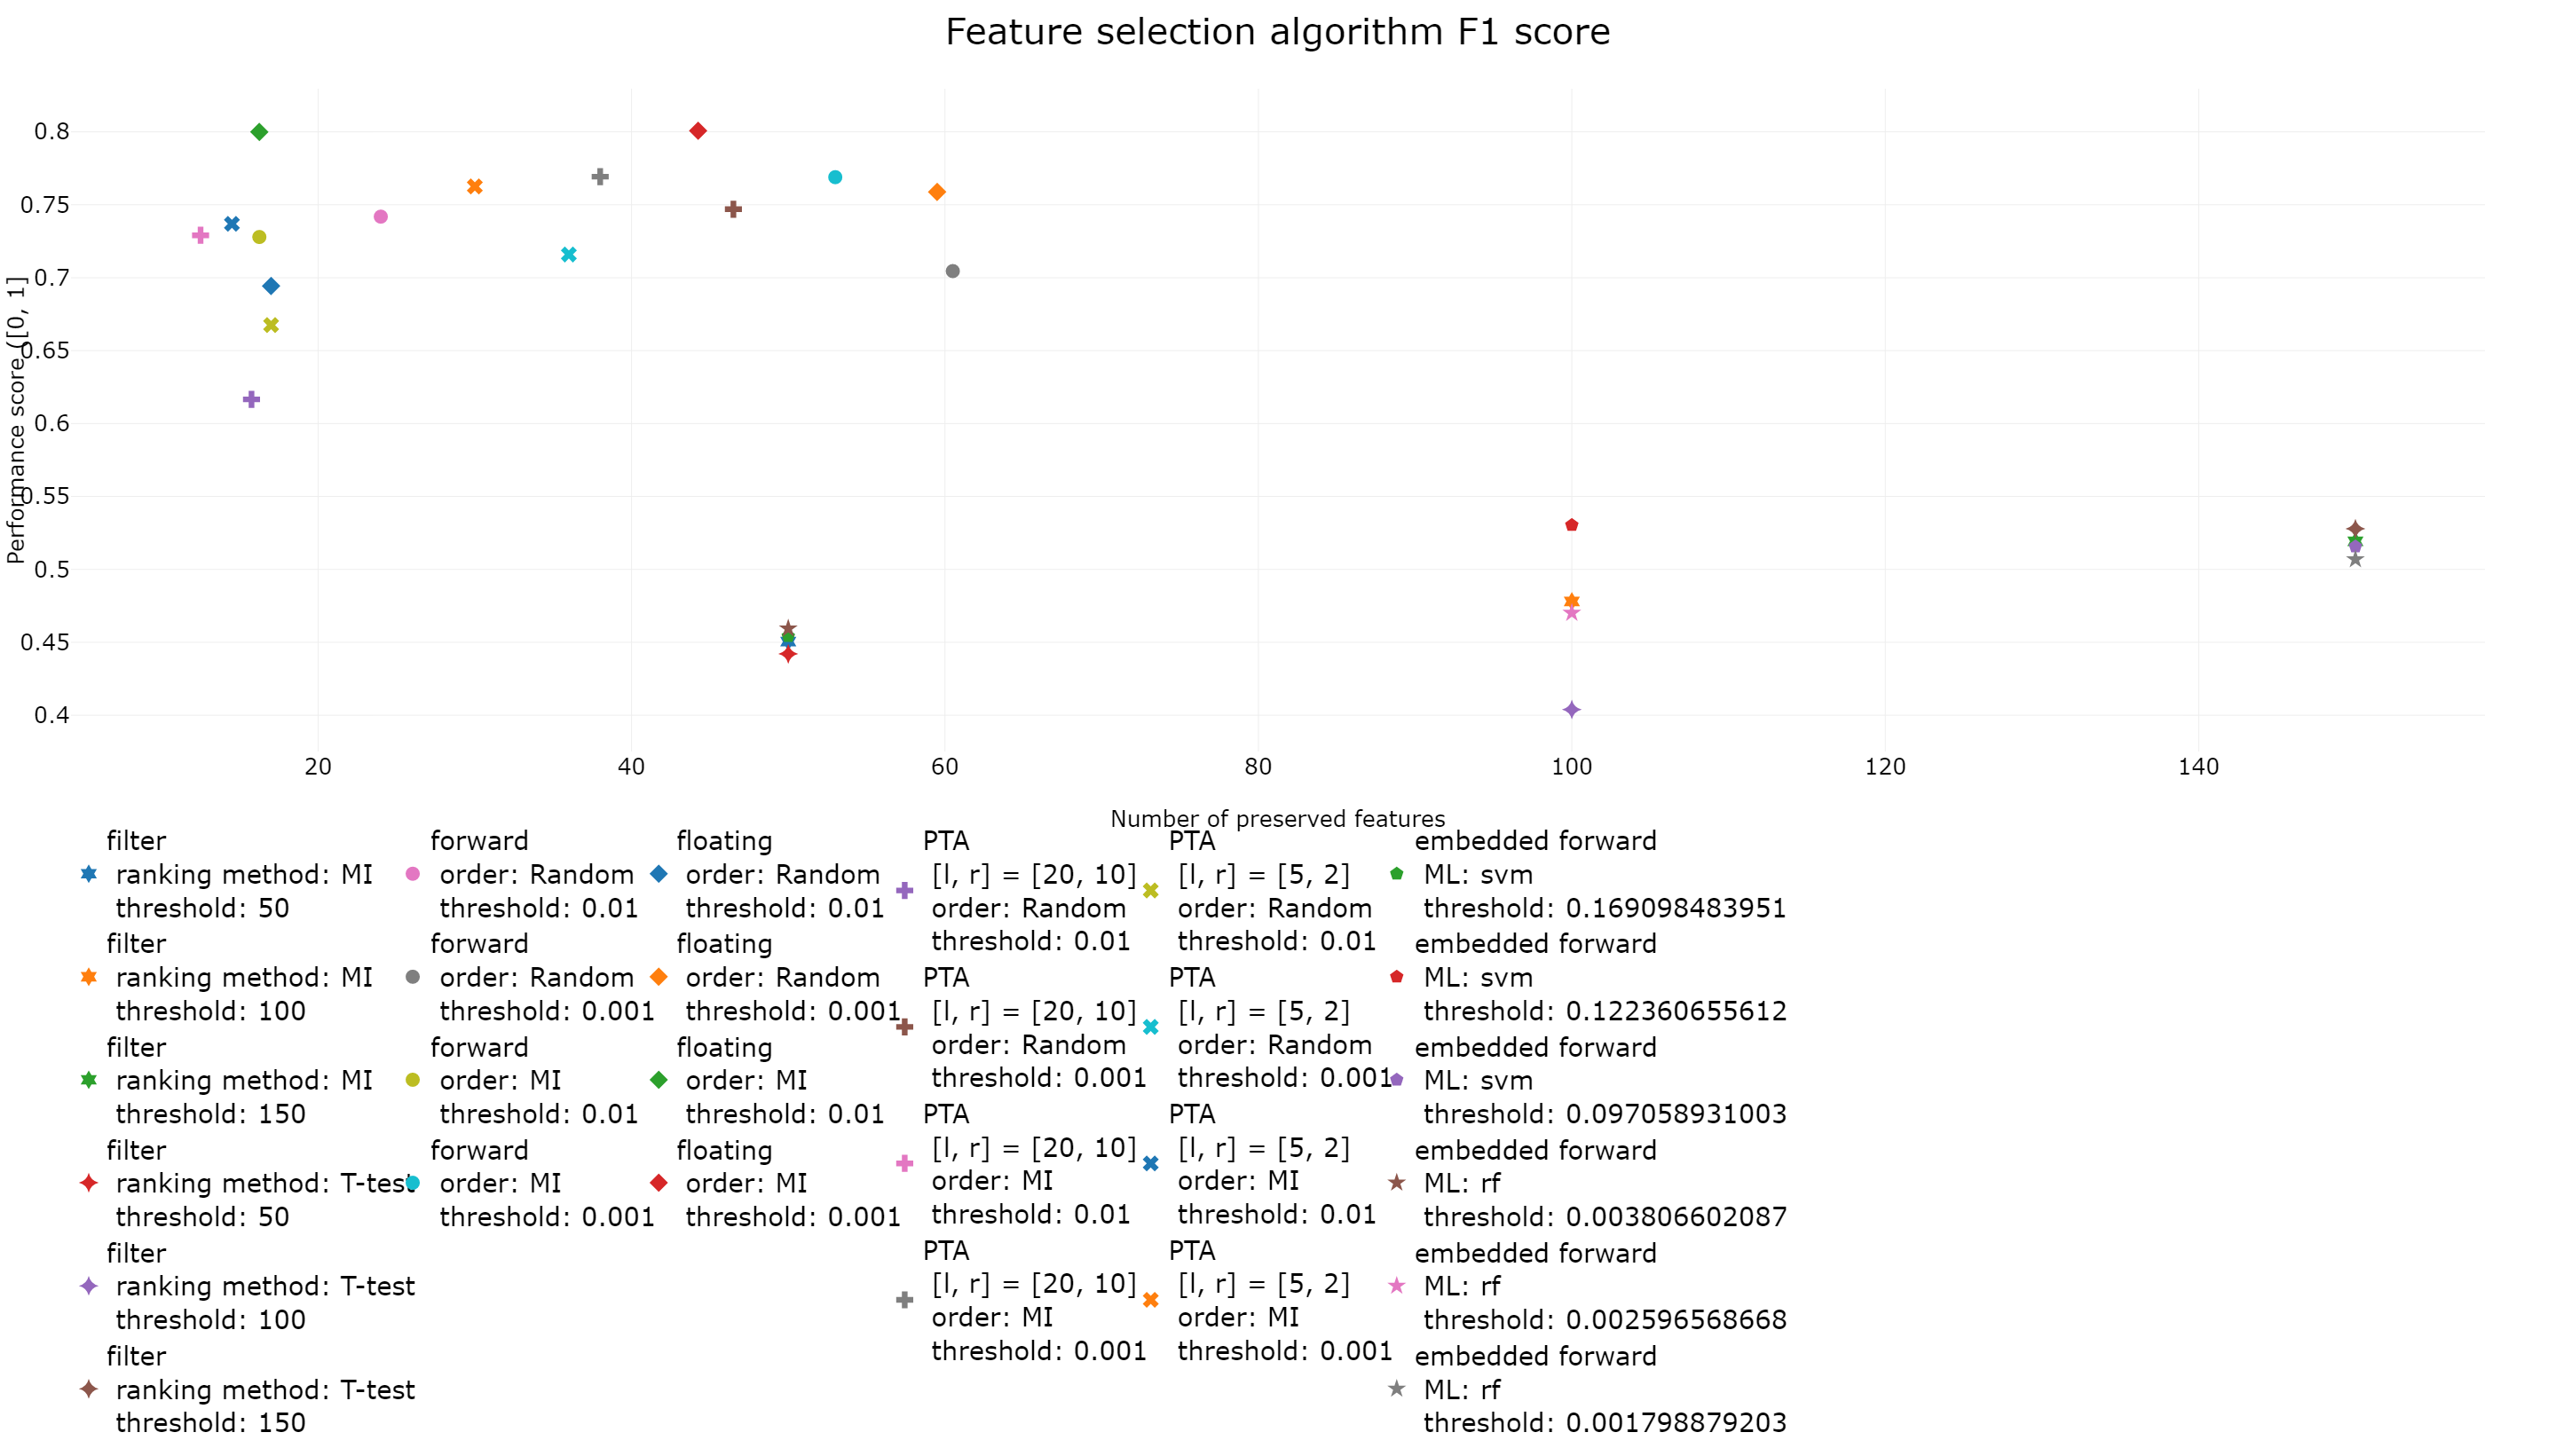
\includegraphics[angle=90,height=1.4\textwidth]{F1_new.png}
		\caption{The F1 spectrum for the average dataset. The x-axis shows the average number of features that are preserved and the y-axis shows the F1 score of logistic regression. The legend indicates the algorithms and their corresponding shapes, as well as the chosen parameters with their matching colours. Abbreviations in legend: Mutual Information (MI), Pick l-Take Away r (PTA), Machine Learning algorithm (ML), Support Vector Machine (svm), random forest (rf)}
		\label{fig:Avg_F1_Spectrum}
	\end{figure}
	
	% Computation time
	Aside from the ability to preserve the correct features, also an evaluation of the computation time was made for the different algorithms (Figure \ref{fig:Comp_Time_Bar}). This chart immediately showed that the wrapper methods took significantly more computation time, with floating search taking the longest time. There was no major difference between forward selection and both PTAs, however there was a difference between filter methods using Mutual Information and T-test. Also for the embedded methods, the SVM based embedded method took significantly less time as well, compared with the random forest embedded method.
	
	% Insert figures
	\begin{figure}[H]
		\centering
		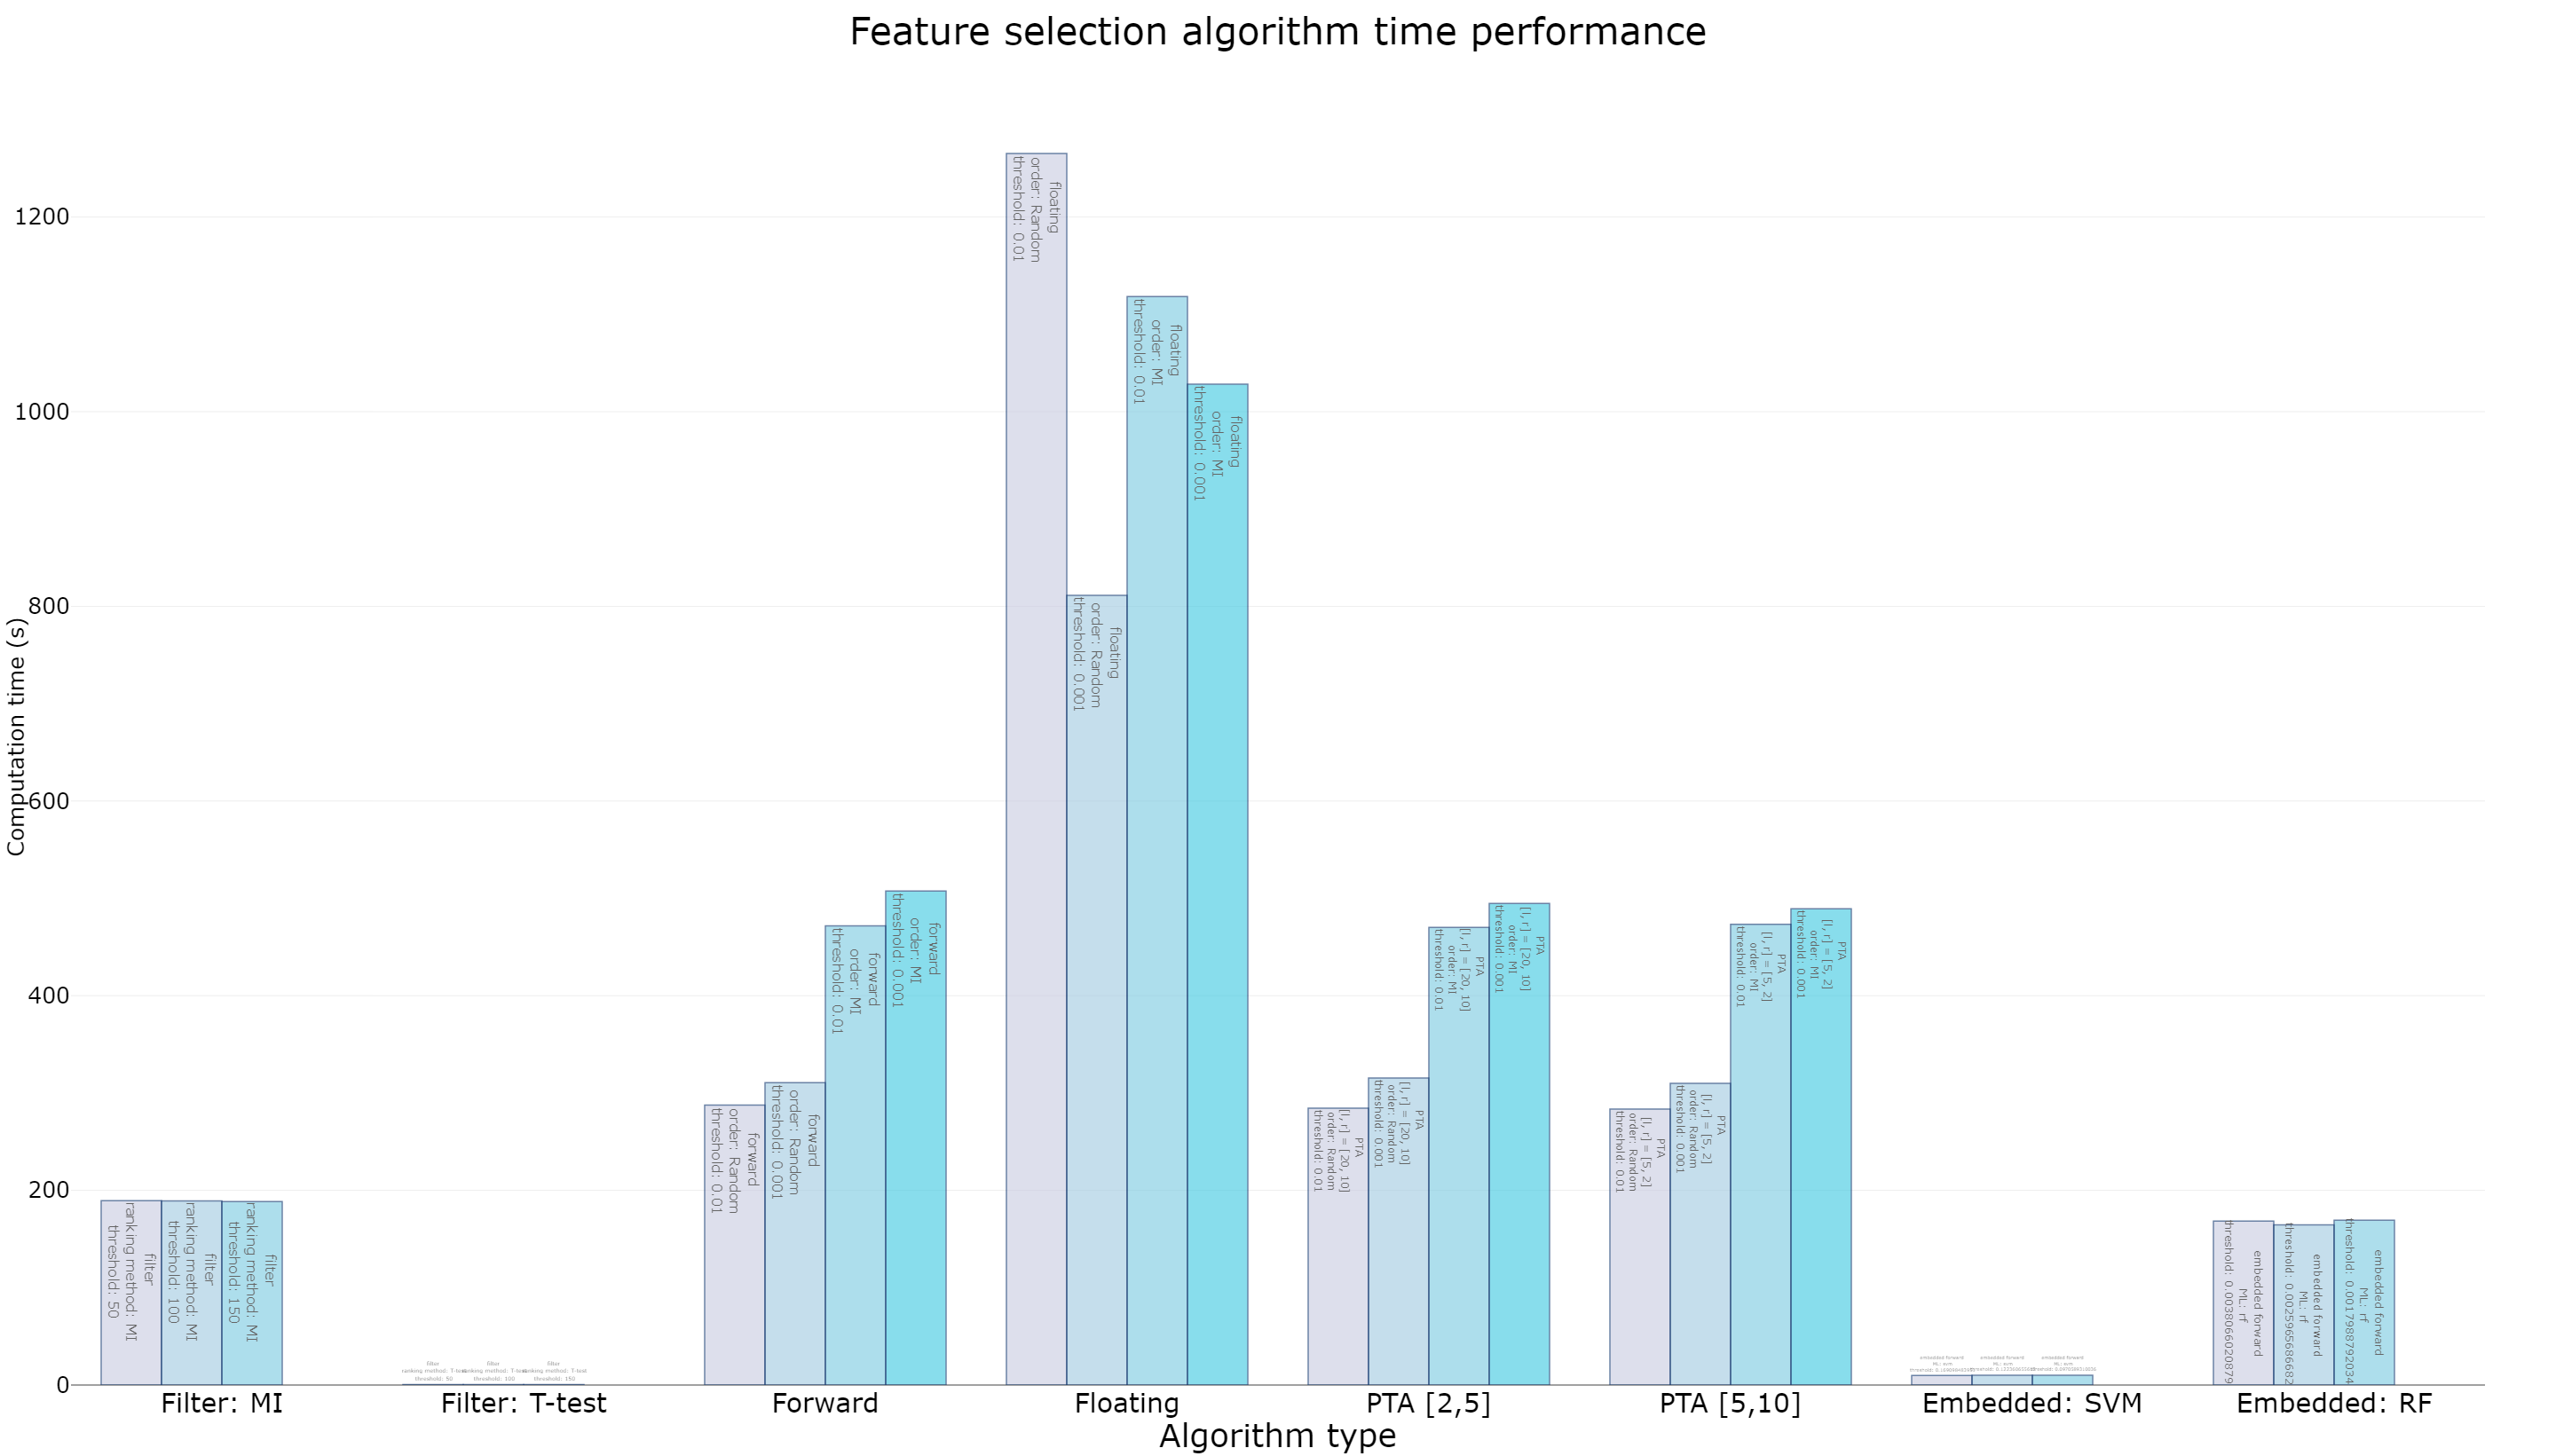
\includegraphics[angle=90,height=1.4\textwidth]{ComputationTimeBarChart.png}
		\caption{A bar chart showing the average computation time of all evaluated algorithms. The x-axis corresponded to the different algorithms, for which the computation time for multiple parameter combinations were given. The y-axis corresponded to the computation time in seconds. Abbreviations in legend: Mutual Information (MI), Pick l-Take Away r (PTA), Support Vector Machine (svm), random forest (rf)}
		\label{fig:Comp_Time_Bar}
	\end{figure}
	
	% FS_Accuracy
	At last the relation between the computation time and \textit{FS\_score}, the corrected accuracy, are visualized (Figure \ref{fig:Comp_Time_FS_Acc}). In this chart the trade-of between computation time and quality of a feature selection algorithm is  shown by the following statements: 
	\begin{itemize}
		\item Filter and embedded methods take the shortest time, but have the worst performance. Floating methods take the longest time, but are not necessarily better than other wrapper methods
		\item For both filter and embedded methods using T-test and SVM over mutual information and random forests respectively seems to greatly reduce computation time for little to no improvement in \textit{FS\_score}.
		\item The addition of an ordering and the choice of a threshold of $\alpha = 0.01$ over $\alpha = 0.001$ gives better results for all wrapper methods. Using these hyper-parameters however usually add computation time.
		\item Forward selection and PTA do not show a big difference compared to each other.
	\end{itemize}
	
	% Insert figures
	\begin{figure}[H]
		\centering
		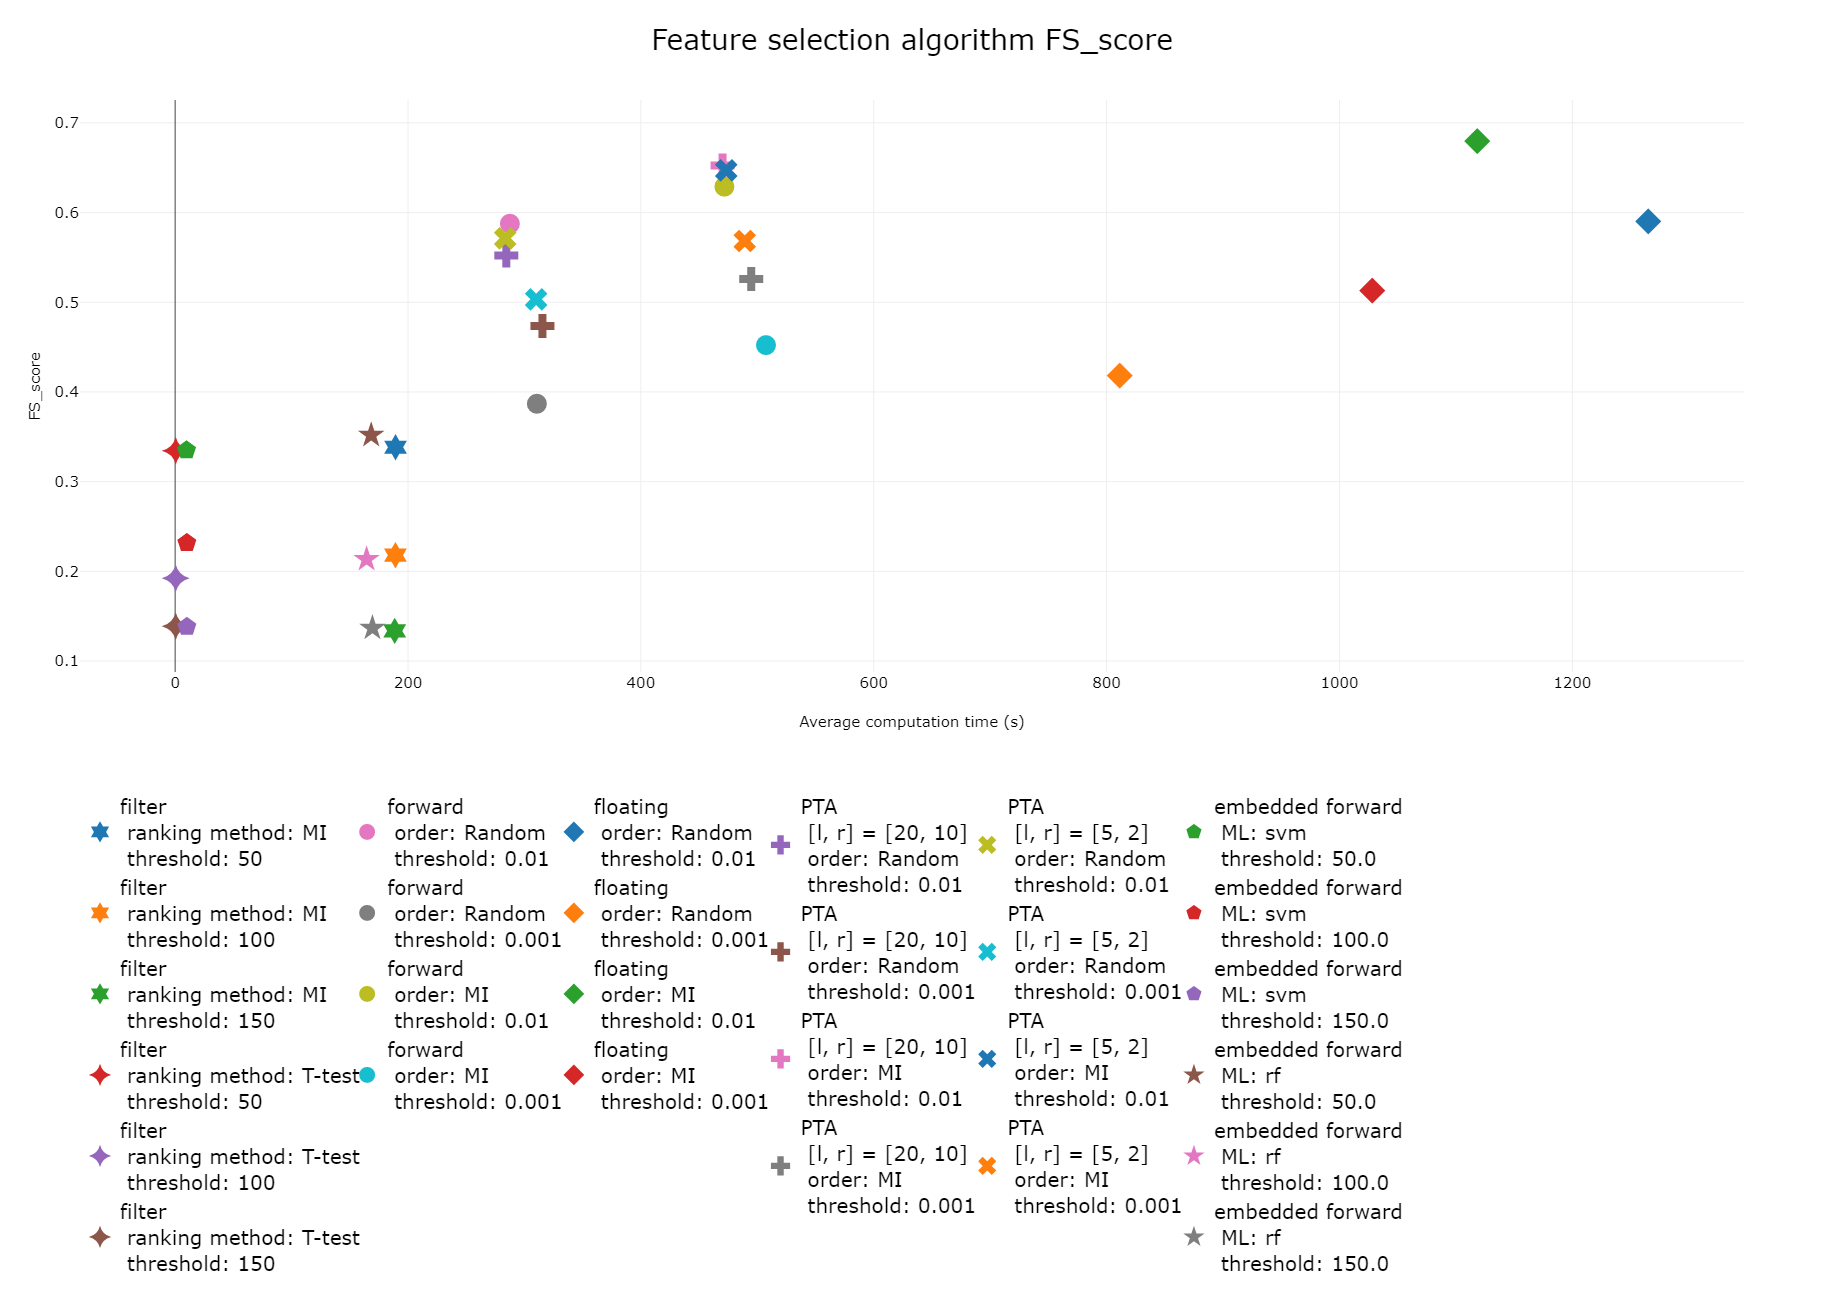
\includegraphics[angle=90,height=1.4\textwidth]{Pareto_FSscore_Comp.png}
		\caption{The relation between the \textit{FS\_score} and the computation time. The x-axis shows the computation time the y-axis shows the \textit{FS\_score} score of logistic regression. The legend indicates the algorithms and their corresponding shapes, as well as the chosen parameters with their matching colours. Abbreviations in legend: Mutual Information (MI), Pick l-Take Away r (PTA), Machine Learning algorithm (ML), Support Vector Machine (svm), random forest (rf)}
		\label{fig:Comp_Time_FS_Acc}
	\end{figure}
	
	\subsection{TPOT Feature Selection Integration Results}
	
	To visualize the results of the experiment, a table with the final results is made (Table \ref{tab:TPOTResults}). The optimization process is also recorded and shown in a plot for the Micro-organisms (Figure \ref{fig:TPOTResultMO}), Arcene (Figure \ref{fig:TPOTResultArcene}), RSCTC (Figure \ref{fig:TPOTResultRSCTC}) and Psoriasis (Figure \ref{fig:TPOTResultPsoriasis}) dataset. The five experiment reruns are averaged to one complete result.
	
	\begin{table}[]
		\caption{The performance of the final pipeline for the different types of \textit{TPOT} and the mentioned dataset. The five reruns are averaged into this one result.}
		\label{tab:TPOTResults}
		\begin{tabular}{ll|ll|ll}
			\multirow{2}{*}{\textbf{Algorithm}} & selection      & \multicolumn{2}{l|}{regular selection}                                                                                                 & \multicolumn{2}{l}{always feature selection}                                               \\ \cline{3-6} 
			& availability   & \begin{tabular}[c]{@{}l@{}}regular\\ algorithms\end{tabular} & \begin{tabular}[c]{@{}l@{}}feature selection\\ algorithms\end{tabular} & regular algorithms & \begin{tabular}[c]{@{}l@{}}feature selection\\ algorithms\end{tabular} \\ \hline
			\multirow{4}{*}{\textbf{Datasets}}  & Micro-organisms & 0.45                                                        & 0.71                                                                  & 0.64               & 0.59                                                                   \\
			& Arcene         & 0.46                                                        & 0.69                                                                  & 0.62               & 0.69                                                                   \\
			& RSCTC          & 0.00                                                       & 0.22                                                                 & 0.17              & 0.44                                                                       \\
			& Psoriasis      & 0.00                                                       & 0.24                                                                 & 0.16                   & 0.54                                                                      
		\end{tabular}
	\end{table}
	
	\begin{figure}[H]
		\centering
		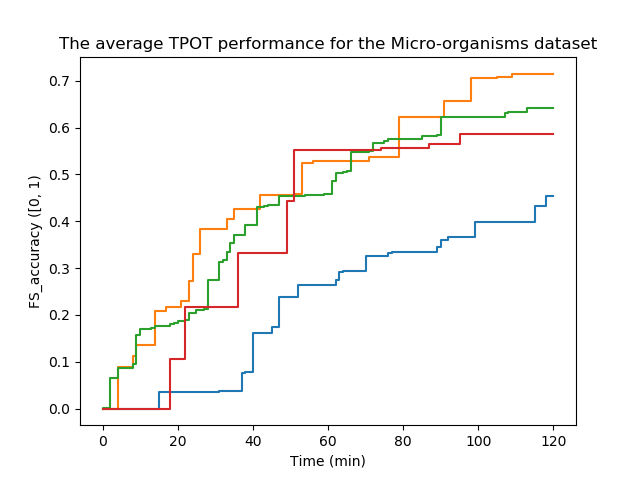
\includegraphics[width=0.8\textwidth]{TPOT_avg_MO.PNG}
		\caption{The optimization process for the different \textit{TPOT} algorithms for the micro-organisms dataset.}
		\label{fig:TPOTResultMO}
	\end{figure}
	
	\begin{figure}[H]
		\centering
		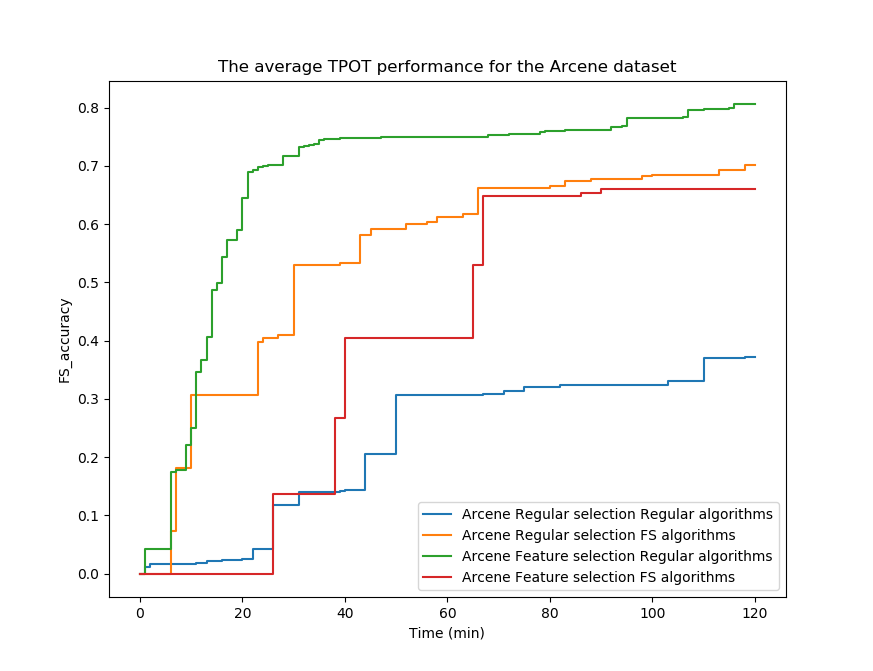
\includegraphics[width=0.8\textwidth]{TPOT_avg_Arcene.PNG}
		\caption{The optimization process for the different \textit{TPOT} algorithms for the Arcene dataset.}
		\label{fig:TPOTResultArcene}
	\end{figure}
	
	\begin{figure}[H]
		\centering
		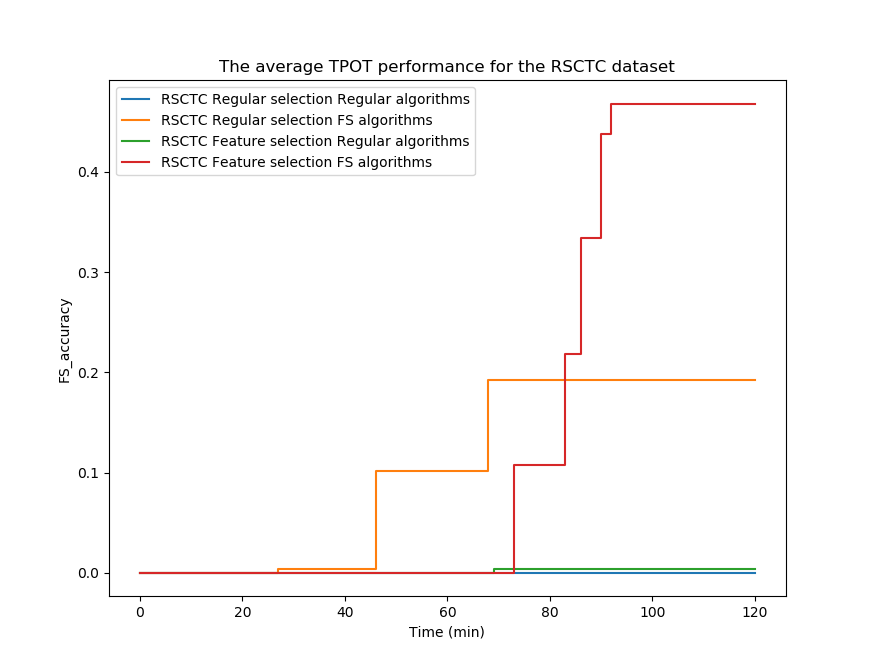
\includegraphics[width=0.8\textwidth]{TPOT_avg_RSCTC.PNG}
		\caption{The optimization process for the different \textit{TPOT} algorithms for the RSCTC dataset.}
		\label{fig:TPOTResultRSCTC}
	\end{figure}
	
	\begin{figure}[H]
		\centering
		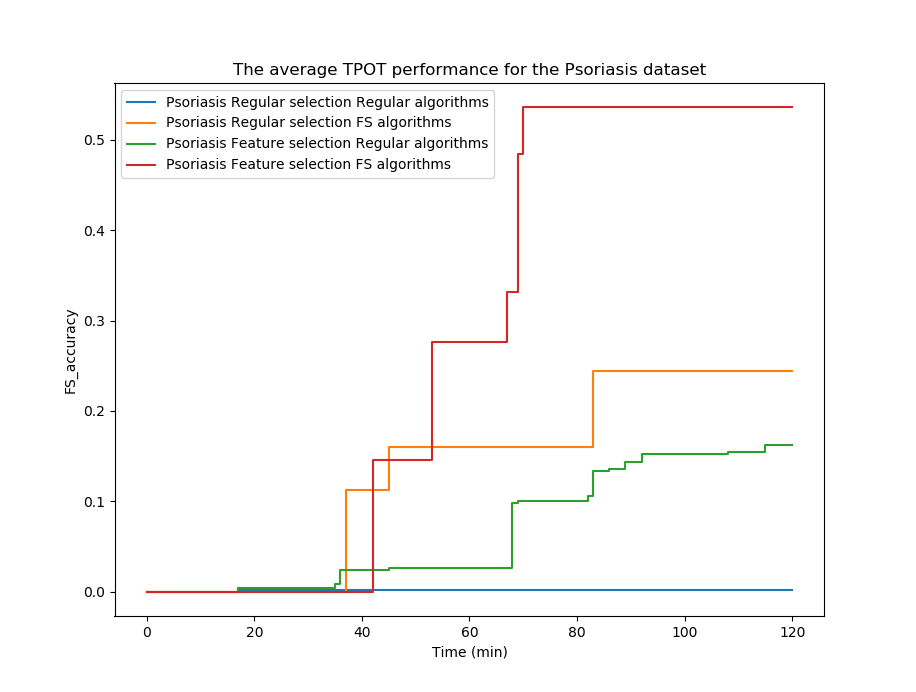
\includegraphics[width=0.8\textwidth]{TPOT_avg_Psoriasis.PNG}
		\caption{The optimization process for the different \textit{TPOT} algorithms for the psoriasis dataset.}
		\label{fig:TPOTResultPsoriasis}
	\end{figure}
	
	% Results \textit{TPOT}
	The results show that after two hours of running \textit{TPOT}, regular \textit{TPOT} always performs worst. According to the processes the high feature selection algorithm set shows much more big stepwise improvements, accompanied with fewer smaller stepwise improvements. This shows the earlier observed trade-off between computation time and feature selection quality for these specific feature selection algorithms. It takes longer to compute those algorithms, but it also gives a much better result. 
	
	% Best \textit{TPOT} type
	The choice for the best \textit{TPOT} algorithm is not conclusive. For high feature selection, all three new possibilities show improved results. The \textit{TPOT} variant that is feature selection focused and has the new feature selection algorithm set performs the best for datasets with a very high number of features (RSCTC and Psoriasis), but the trade-off in computation time seems to hurt the performance for smaller datasets. The algorithm that is only feature selection focused has a steady performance for datasets with a lower number of features, but this performance does not seem to be better than the algorithm with only the new feature selection algorithm set.
	
	\newpage
	\section{Discussion}
	\label{FSsec:Discussion}
	
	% Research relevance
	There are several works focused on the possibility of feature selection, both with a data analytical \cite{catal2009investigating} as well as a biomedical \cite{baumgartner2006data, welthagen2005comprehensive, liu2002comparative} point of view. These research projects are usually focused on datasets with a low number of features, for which feature selection is less relevant. This research for datasets that have a significantly higher number of at least 1000 features is new, even though newly available datasets become bigger over time due to new and improved techniques of measuring and storing data. With this research a beginning is made on how to approach feature selection on these bigger datasets.
	
	% Wrapper methods exclusion
	Whereas multiple feature selection methods are discussed, several were not tested due to computation time constraints. The wrapper methods backwards elimination and simulated annealing and the embedded backwards elimination all were too computationally intensive to become relevant for the research. In datasets with fewer features, these methods may be showing better results and could be possible candidates for feature selection.
	
	
	\section{Conclusions}	
	\label{FSsec:Conclusions}
	
	% Filter method exploration
	After evaluation of the results in the first experiment set-up, it could be concluded that there was not a big difference between using T-test/ANOVA or Mutual Information as a ranking method. Both gave similar results, with the exception of one dataset (Figure \ref{fig:DatasetRankScores}). T-test/ANOVA was computationally faster than Mutual Information as was seen in the second experiment (Figure \ref{fig:Comp_Time_Bar}), however T-test/ANOVA also worked with the assumption that the classes are normally distributed. This was not always the case. A rule of thumb for choice of ranking method would be to use T-test /ANOVA, except for when the data was not normally distributed. % Both of them should definitely be considered to be used in the framework.
	
	% Second conclusion exploration
	A second conclusion was drawn from looking at the accuracy with the number of features preserved. After a threshold of 200 features, additional features did not raise the validation score as much as the first 200 features did. This indicated a second rule of thumb, that at least 200 features should be preserved after using a filter method. This rule of thumb was according to the hypothesis H1 notion that at most 1000 features should be preserved to still show an efficient result, however was much lower than the expected upper bound of 1000 features. This absolute number was not intuitive and much lower than expected. More research could be done on these preserved 200 features and why no other features were needed to predict the output. Cluster analyses for example may show insights in this phenomenon.
	
	% Second experiment - filter vs wrapper methods
	After evaluation of both filter, wrapper and embedded methods, wrapper methods were significantly better at selecting a smaller fraction of features while preserving a similar test score.  Whereas hypothesis H2 stated wrapper methods to be best in efficiency, embedded methods were expected to outperform both filter methods and wrapper methods when looking at both quality and computation time. This was not the case, however, as embedded methods had a near identical quality to filter methods and performed much worse than wrapper methods. The outcome indicated that wrapper methods are significantly different in results and filter and embedded methods being nearly identical.
	
	% Further conclusions
	Since wrapper methods take dependencies between features into account, they kept these dependencies at a minimum. If these dependencies are unwanted, wrapper methods are more useful than filter methods and embedded and should be recommended. A downside of the wrapper methods however was that they took much more computation time than the filter and embedded methods. Therefore if it does not matter when features have dependencies with each other, a filter method should be recommended.
	
	% Wrapper methods with each other
	There was a difference in quality within the wrapper methods. The forward selection and PTA all showed promising results and therefore should be considered for the framework. Floating search showed the best results, however took significantly longer in computation time. Within the wrapper methods, an ordering beforehand showed improved results. Backward elimination wrapper algorithms, stochastic search algorithms and embedded backwards elimination algorithms all were significantly worse in computation time than the other wrapper algorithms and therefore should not be considered in these cases.
	
	% Threshold wrapper methods
	A recommendation for the threshold in wrapper methods is not trivial. A higher threshold of $\alpha = 0.01$ gave a smaller feature subset at the cost of a lower classification score. If a smaller subset is desired or more influential features are needed, a bigger threshold should be chosen, whereas it will be smaller when a higher quality of the feature subset is desired.
	
	% Combinations
	In this research only separate feature selection methods were tested. Whereas the filter methods used very little computation time, the feature subset size and quality of the wrapper methods were much more interesting for further research. A combination of a filter and a wrapper method might create a better result. If first the majority of the features is filtered out by a filter method and then a wrapper method computes the best combination of feature, the result can be relatively quicker than the wrapper method while still maintaining a high enough quality. This combination is worth investigating in future research.
	
	% \textit{TPOT} conclusion
	Both additions to \textit{TPOT} were beneficial according to the experiment. This was also expected, as H3 states.  When the initial number of features was very high (50.000), a combination of initial bias towards feature selection and using feature selection algorithms focusing on preservation of only 200 features performed best. For lower number of features only adding one of the improvements was better, as computation time became the limiting factor in case of using both improvements.

	\chapter{Missing Value Handling}
	\label{chap:MissingValueHandling}
	
	\section{Introduction}
	\label{MVsec:Introduction}
	
	% Lowered quality: Missing values and outliers
	The quality of data should be as high as possible. Data values however could be missing, for example due to patients not showing up or because of mistakes by the medical staff. Missing values hinder the data set quality significantly and for numerous datasets removing or replacing them would significantly help to increase the quality of the research. Several works already focused on the handling of missing values \cite{donders2006gentle, cartwright2003dealing, haukoos2007advanced}. A biomedical data analysis framework would benefit from the possibility to remove or replace missing values. Therefore the research goal for this project is \emph{to evaluate the performance of missing value handling methods and make a choice on which methods should be added to the framework}. Therefore in this document several of those algorithms are presented and tested on their quality.
	
	\section{Background}
	\label{sec:Background}
	
	\subsection{Datasets}
	\label{MVsubsec:Datasets}
	
	% Introduction
	A total of four datasets were used for the analysis of missing values. Three of these datasets are clinical data and one of them is survey data (Subsection \ref{PLsec:Datasets}). The specifications of the four datasets are summarized together (Table \ref{tab:Datasets}).
	
	\begin{table}[H]
		\caption{A schematic overview of the four datasets}
		\label{tab:Datasets}
		\resizebox{\textwidth}{!}{%
			\begin{tabular}{l|lll|lll|l}
				\textbf{Dataset focus} & \textbf{Features} & \textbf{Samples} & \textbf{Classes} & \textbf{\begin{tabular}[c]{@{}l@{}l@{}}Total \\ Missing \\ values (\%)\end{tabular}} & \textbf{\begin{tabular}[c]{@{}l@{}l@{}}Most missing\\ in single \\ feature (\%)\end{tabular}} & \textbf{\begin{tabular}[c]{@{}l@{}l@{}}Features\\ with missing\\ values\end{tabular}} & \textbf{Remarks}                                                                                                                            \\ \hline
				\textbf{Heart attack}           & 9                 & 108              & 53               & 8.29\%                                                                 & 43.85\%                                                                         & 7 & \begin{tabular}[c]{@{}l@{}}- Output in months\\ (Regression preferred)\\ - Values are missing \\ due to time constraints\\ ---\end{tabular} \\
				\textbf{Hepatitis}              & 19                & 155              & 2                & 5.67\%                                                               & 43.22\%                                                                         & 15 & \begin{tabular}[c]{@{}l@{}}- Used in previous \\ published studies\\ ---\end{tabular}                                                       \\
				\textbf{Cirrhosis}              & 18                & 1945             & 3                & 3.24\%                                                               & 42.21\%                                                                        & 6 & \begin{tabular}[c]{@{}l@{}}- Missing not \\ completely at random\\ ---\end{tabular}                                                         \\
				\textbf{Cervical Cancer}        & 28                & 858              & 5                & 15.07\%                                                               & 91.72\%                                                                        & 26 & \begin{tabular}[c]{@{}l@{}}-  Missing values mainly \\ from the survey part\\ - Output comprised of \\ four separate indicators\end{tabular}
			\end{tabular}
		}
	\end{table}
	
	\subsection{Missing Value Handling}
	\label{MVsubsec:MissingValueHandling}
	
	% Introduction
	Numerous reasons can cause entries to be missing from a dataset. A sample can be missing, corrupted or contaminated, a measurement malfunction can occur, a patient can fail to show up at a scheduled meeting or not respond to a survey. These missing entries are different on both origin and possibly also on randomness. This also indicates that techniques differ in effectiveness on missing values caused by separate reasons. Therefore the different types of missing values will be explained, as well as techniques to cope with these missing values.
	
	% Responsiveness
	Since there are multiple steps to be taken for gathering data, a problem during an earlier step can generate more values to be missing. When a patient fails to come to the hospital for a second round of tests all values for the second test are absent, whereas a nurse accidentally skipping to note the weight of a patient will only cause the absence of one value. A difference is therefore made between item and unit non-responses. An item response is a single missing value in a data set and a unit non-response corresponds to a series of missing values. \cite{patrician2002multiple}
	
	% Randomness aspect of mising value
	Another aspect of missing values is its randomness. A missing value can occur completely random without any relation with other values, however it is not uncommon to have some relation with another value. Three different types of randomness are defined to explain this. The first type is \textit{missing completely at random} (MCAR) \cite{donders2006gentle,cartwright2003dealing, haukoos2007advanced}, and means that missing entries have no relation with any part of the data. This means removing samples with missing values should not create any bias in the resulting dataset. An example would be accidentally dropping a blood vial, not being able to report the blood values. The opposite of MCAR is \textit{missing not at random} (MNAR) \cite{donders2006gentle, haukoos2007advanced}, also known as \textit{non ignorable} (NI) \cite{cartwright2003dealing}. MNAR means that missing values are linked to the feature they are missing from, which makes it very difficult to find the relation between the missingness and a feature. Examples with MNAR values are patients that are unsuccessfully treated for a disease, and are therefore less likely to return for future tests, creating a bias in the values about disease severity. In between MCAR and MNAR is \textit{missing at random} (MAR) \cite{donders2006gentle,cartwright2003dealing, haukoos2007advanced}. MAR indicates missing entries that have no relation with the feature they are missing from, but have a relation with other features in the data sets. These entries can be estimated using the relation to better identify a possible value. Examples are specific diagnostic tests that are done for patients of a specific disease for increased health risks, whereas other (healthy) subjects were not tested \cite{haukoos2007advanced}. Whereas MCAR values are relatively easy and MNAR values are almost impossible to cope with, MAR values can be treated properly with complex approaches so proper values are imputed in those cases. Therefore many imputation techniques are created on basis of the MAR assumption.
	
	% Introduction different  coping techniques
	The techniques of coping with missing values are based on three approaches. The first principle is list deletion (LD) \cite{donders2006gentle, haukoos2007advanced}, deleting samples, features or both to create a smaller dataset without missing values. This is the most common way to treat missing values as it is quick and easy. If enough samples are present and there is not too much bias between samples including and excluding missing values, this is the way to go. If the number of samples is limited or a bias is present in the missing value samples, value imputation becomes more interesting. In this case valuable information will not be omitted and the possible bias is taken into account. Imputation can be split into two different types, single imputation (SI) \cite{donders2006gentle, cartwright2003dealing, haukoos2007advanced} and multiple imputation (MuI) \cite{donders2006gentle, patrician2002multiple, sterne2009multiple}. Thirdly, instead of removing or adding values, the dataset can be directly used in a model, disregarding missing values in the model \cite{myrtveit2001analyzing}. Since methods handling missing values can usually be best explained by showing example algorithms, several pseudo-algorithms were created for visual clarity.
	
	% Pseudo-algorithms
	
	
	\subsubsection{List Deletion}
	\label{MVsubsec:ListDeletion}
	
	% Introduction
	List deletion (LD) is a quick and easy manner to perform for coping with missing values. Samples or features are removed when they consist of at least one missing value until no more missing values are present. Three difference approaches are explained: \textit{complete case analysis} (CCA), \textit{available case analysis} (ACA) and \textit{weighted case analysis} (WCA).
	
	\begin{itemize}
		
		% Complete case analysis
		\item \textit{Complete case analysis} \\
		CCA is the most basic LD approach. CCA removes all samples that have missing values and therefore prepares only complete samples for future analysis (Algorithm \ref{alg:ACA}). The dataset should consist of a reasonable number of complete samples to leave enough data for analysis. Also data should be MCAR, as removing cases that have a dependency with certain features can create a bias. CCA is most used as a way of removing missing values, even though not every time MCAR is available \cite{haukoos2007advanced, patrician2002multiple, myrtveit2001analyzing, donders2006gentle}. In those cases CCA is proven to be biased \cite{cartwright2003dealing}.
		
		\begin{algorithm}[H]
			\caption{Complete Case Analysis}\label{alg:CCA}
			\begin{algorithmic}[1]
				\Procedure{CCA($X$)}{}
				\State $S \gets \text{range(\#rows(X))}$ 	\Comment{Create a list of all samples}
				\For {$s \textbf{ in } S$} 					\Comment{For all samples in $S$}
				\If {$\textit{missing\_values}(X_s) \textbf{ is } \text{True}$} 				\Comment{find out if missing values are present} 			
				\State $\textbf{remove } X_s \textbf{ from } X$ 				\Comment{Remove the sample with missing values}
				\EndIf
				\EndFor
				\State $\textbf{return X}$
				\EndProcedure
			\end{algorithmic}
		\end{algorithm}	
		
		% Available case analysis
		\item \textit{Available case analysis} \\
		ACA tries to preserve more samples by only using useful features. ACA first makes a selection on relevant features in the dataset. Those features are selected by hand so they will be present in future analysis. A second approach is to remove features for which the percentage of missing values is higher than a threshold $\alpha$. After selecting those features, samples without missing values in the relevant feature set are kept, all others are removed (Algorithm \ref{alg:ACA}). This is similar to CCA, but will preserve more samples if several features have significantly more missing values. For this LD, MCAR would be desired. However if either the MAR values or the features it has a relation with are removed, there will be no relation between the MAR values and the dataset any more and therefore no bias will be created \cite{haukoos2007advanced, donders2006gentle, patrician2002multiple, myrtveit2001analyzing}. Often though, this will not be the case, as the dependency is on either a multitude of features and the dependent feature is important for the research.
		
		\begin{algorithm}[H]
			\caption{Available Case Analysis}\label{alg:ACA}
			\begin{algorithmic}[1]
				\Procedure{ACA($X$, $\alpha$)}{} 
				\State $F \gets \text{range(\#columns(X))}$ 	\Comment{Create a list of all samples}
				\For {$f \textbf{ in } F$} 					\Comment{For all features in $F$}
				\If {$\textit{perc\_missing\_values}(X_f) > \alpha$} 				\Comment{\textit{perc\_missing\_values} finds out the percentage of missing values} 			
				\State $\textbf{remove } X_f \textbf{ from } X$ 				\Comment{Remove the feature with too many missing values}
				\EndIf
				\EndFor
				\State $\textbf{return CCA(X)}$
				\EndProcedure
			\end{algorithmic}
		\end{algorithm}	
		
		% Weighted case analysis -> Interesting for unit non responsiveness
		\item \textit{Weighted case analysis} \\
		A third type of LD is WCA. WCA tries to overcome bias from CCA by assigning 
		weights to every value (Algorithm \ref{alg:WCA}). If a sample is removed, 
		the nearest complete neighbour is searched for (Algorithm \ref{alg:WCA} -  
		row 5). This closest complete sample can be found by using one, multiple or 
		available features. The complete sample is then given a higher weight 
		corresponding to the number of closest omitted samples. A simple approach 
		for giving a higher weight is simply by adding an additional complete case 
		to the existing complete cases, choosing the one that is closest to the 
		incomplete case. This technique tries to remove the bias as much as 
		possible by maintaining the distribution of the samples. This technique 
		specifically does not assume MCAR values, but MAR 
		values \cite{haukoos2007advanced, donders2006gentle}. Also this 
		technique is specifically useful for unit non-responsiveness for its 
		simplicity to cope with multiple missing values in one 
		sample \cite{patrician2002multiple}.
	\end{itemize}
	
	\begin{algorithm}[H]
		\caption{Weighted Case Analysis}\label{alg:WCA}
		\begin{algorithmic}[1]
			\Procedure{WCA($X$)}{} 
			\State $S \gets \text{range(\#rows(X))}$ 	\Comment{Create a list of all samples}
			\For {$s \textbf{ in } S$} 					\Comment{For all samples in $S$}
			\If {$\textit{missing\_values}(X_s) \textbf{ is } \text{True}$} 				\Comment{find out if missing values are present} 			
			\State $s_{nn} = \textit{nearest\_complete\_neighbour(X, s)}$	\Comment{Find the nearest complete neighbour of $s$}
			\State $ X_s \gets X_{s_{nn}}$ 				\Comment{Change the values of $s$ to the values of $s_{nn}$}
			\EndIf
			\EndFor
			\State $\textbf{return X}$
			\EndProcedure
		\end{algorithmic}
	\end{algorithm}	
	
	% Advantages and disadvantages
	Whereas List Deletion is used most regularly and is quickest and easiest of all the missing value handling techniques, it is often criticized for its drawbacks. If the data is not MCAR, bias will most often be created, even in ACA and WCA \cite{cartwright2003dealing}. Also the removal of samples is not always desired when not many samples were available at the start \cite{haukoos2007advanced, myrtveit2001analyzing, donders2006gentle}. All things considered LD is a quick fix when needed. For better understanding of the data however, other approaches seem more appropriate.
	
	\subsubsection{Single Imputation}
	\label{MVsubsec:SingleImputation}
	
	% Introduction
	An intuitive approach of coping with missing values and not wanting to delete entire samples or features is to impute an appropriate entry in its place. If the imputed entry is a proper representation of all possible entries, the possibly valuable information within the sample or feature will be useful for data analysis. Imputing a replacement value for the missing value is called Single Imputation (SI). Several different approaches for SI are known and used. \cite{haukoos2007advanced, donders2006gentle, myrtveit2001analyzing}
	
	
	\begin{itemize}
		% Missing indicator method
		\item \textit{Missing indicator method} \\
		The simplest way of SI is missing indicator method. This approach imputes a generic variable for every missing value of a feature, for example imputing $0$ for heart rate for every missing measurement. Aside from that, it also creates an additional boolean feature that indicated whether a value was missing or not (Algorithm \ref{alg:MissingIndicatorImputation}). When using a generic feature no additional information is added to the data and no assumptions are made, which makes this method less dependent on assumptions \cite{pedersen2017missing}. Another possibility is to combine the missing indicator method with other imputation methods, for example the mean imputation, so from the dataset missing values can still be traced back. Any calculations or modelling done with the feature has an important dependency to the newly created missing value feature, though. Also if data is MAR and not MCAR, bias may be present due to worse representation \cite{donders2006gentle}.	
		
		\begin{algorithm}[H]
			\caption{Missing Indicator Imputation}\label{alg:MissingIndicatorImputation}
			\begin{algorithmic}[1]
				\Procedure{missing\_indicator\_imputation($X$, $a$)}{} 
				\State $S \gets \text{range(\#rows(X))}$ 	\Comment{Create a list of all samples}
				\State $F \gets \text{range(\#columns(X))}$ 	\Comment{Create a list of all features}
				\For {$f \textbf{ in } F$} 					\Comment{For all features in $F$}
				\If {$\textit{missing\_values}(X_f) \textbf{ is } \text{True}$} 				\Comment{find out if missing values are present} 			
				\State $\textbf{append } X_{f'} \textbf{ to } X$	\Comment{Create a missing indicator feature for $f$}
				\For {$s \textbf{ in } S$} \Comment{For all samples in $S$}
				\If {$\textit{missing\_values}(X_{s,f}) \textbf{ is } \text{True}$} 				\Comment{Find out if missing} 
				\State $X_{s,f} \gets a$	\Comment{Impute generic value for missing vlaue}
				\State $X_{s,f'} \gets True$	\Comment{Assign true for missing indicator value}
				\Else
				\State $X_{s,f'} \gets False$ \Comment{Assign false for missing indicator value}
				\EndIf
				\EndFor
				\EndIf
				\EndFor
				\State $\textbf{return X}$
				\EndProcedure
			\end{algorithmic}
		\end{algorithm}
		
		% Mean/Median/Mode imputation
		\item \textit{Mean/Median/Mode imputation} \\
		The values of a feature usually follow a certain distribution. In a continuous distribution values are most probable to be the mean of the distribution. Therefore if a value should be imputed, the mean would be the most logical imputation (Algorithm \ref{alg:MeanImputation}). For ordinal features this would be the median and for categorical the mode \cite{haukoos2007advanced, myrtveit2001analyzing, cartwright2003dealing}. With this imputation the distribution centre stays the same, but the standard error is lowered due to addition of new values. This creates a bias for the variance of the feature. Moreover if the data is MAR and not MCAR, additional bias will be created. The original and imputed values combined will then not be a representation of the total number of values \cite{donders2006gentle, pedersen2017missing}.
		
		\begin{algorithm}[H]
			\caption{Mean Imputation}\label{alg:MeanImputation}
			\begin{algorithmic}[1]
				\Procedure{mean\_imputation($X$)}{} 
				\State $S \gets \text{range(\#rows(X))}$ 	\Comment{Create a list of all samples}
				\State $F \gets \text{range(\#columns(X))}$ 	\Comment{Create a list of all features}
				\For {$s \textbf{ in } S, f \textbf{ in } F$} 					\Comment{For all samples in $S$ and features in $F$}
				\If {$\textit{missing\_values}(X_{s,f}) \textbf{ is } \text{True}$} 				\Comment{find out if missing values are present} 			
				\State $X_{s,f} \gets \textit{mean}(X_f)$	\Comment{Assign the mean of the values for feature $f$}
				\EndIf
				\EndFor
				\State $\textbf{return X}$
				\EndProcedure
			\end{algorithmic}
		\end{algorithm}	
		
		% Hot deck
		\item \textit{Hot deck imputation} \\
		Whereas the application of hot deck imputations differs somewhat \cite{myrtveit2001analyzing, cartwright2003dealing, haukoos2007advanced}, the main concept is based on randomly picking a value from a set of possibilities. The set can be all known possible values for the feature, known from other samples in the dataset (Algorithm \ref{alg:HotDeckImputation}). Another approach would be to assume the feature is distributed a specific way (for example normally distributed) and randomly pick a value using the values from that distribution. A third possibility is to combine this with kNN imputation and randomly pick a value from the $k$ nearest neighbours. Randomly picking a value instead of calculating a fixed value will not unjustifiably reduce the variance of the distribution. On the other hand, it also makes the estimation to be more imprecise, possibly creating bias this way \cite{haukoos2007advanced}.
		
		\begin{algorithm}[H]
			\caption{Hot Deck Imputation}\label{alg:HotDeckImputation}
			\begin{algorithmic}[1]
				\Procedure{hot\_deck\_imputation($X$)}{} 
				\State $S \gets \text{range(\#rows(X))}$ 	\Comment{Create a list of all samples}
				\State $F \gets \text{range(\#columns(X))}$ 	\Comment{Create a list of all features}
				\For {$s \textbf{ in } S, f \textbf{ in } F$} 					\Comment{For all samples in $S$ and features in $F$}
				\If {$\textit{missing\_values}(X_{s,f}) \textbf{ is } \text{True}$} 				\Comment{find out if missing values are present} 			
				\State $X_{s,f} \gets \textit{random}(X_f)$	\Comment{Assign a random choice of the values for feature $f$}
				\EndIf
				\EndFor
				\State $\textbf{return X}$
				\EndProcedure
			\end{algorithmic}
		\end{algorithm}	
		
		% Multivariable regression imputation
		\item \textit{Multi-variate regression imputation} \\
		Instead of only using information of the feature that has missing values, other features can be used to predict the missing value replacements. Especially when multicollinearity is present, a prediction of the actual missing value can be computed quite precisely. A multivariate regression model can be made by using features without missing values as input and the features with missing values as output. For example, with linear regression a function can be made between the input and output, trained by all available values and used for predicting all missing values (Algorithm \ref{alg:RegressionImputation}) \cite{raghunathan2001multivariate}. This approach is especially suited for MAR values, in which the absence of feature values is related with other features. The regression imputation should be used with care, as it is unwise to be used if afterwards a similar regression technique is used for further analysis \cite{donders2006gentle}.
		
		\begin{algorithm}[H]
			\caption{Multivariate Regression Imputation}\label{alg:RegressionImputation}
			\begin{algorithmic}[1]
				\Procedure{regression\_imputation($X$)}{} 
				\State $S \gets \text{range(\#rows(X))}$ 	\Comment{Create a list of all samples}
				\State $F \gets \text{range(\#columns(X))}$ 	\Comment{Create a list of all features}
				\For {$f \textbf{ in } F$} 					\Comment{For all  features in $F$}
				\If {$\textit{missing\_values}(X_{f}) \textbf{ is } \text{True}$} 				\Comment{Find out if missing values are present} 			
				\State $\textbf{create } \textit{regressor}$	\Comment{Initialize a regressor}
				\State $\textbf{ fit } \text{regressor} \textbf{ with } X_{F \backslash\{f\}}, X_f$	\Comment{Fit the regressor by using other features as input and the feature with missing values as output}
				\For {$s \textbf{ in } S$} \Comment{For all samples in $S$}
				\If {$\textit{missing\_values}(X_{s,f}) \textbf{ is } \text{True}$} \Comment{If a missing value is present}
				\State $X_{s,f} \gets \textbf{with }\textit{regressor} \textbf{ predict } X_{s, F \backslash \{f\}}$ \Comment{Impute a predicted value}
				\EndIf
				\EndFor
				\EndIf
				\EndFor
				\State $\textbf{return X}$
				\EndProcedure
			\end{algorithmic}
		\end{algorithm}	
		
		% KNN imputation
		\item \textit{k-Nearest Neighbour imputation} \\
		Similarly to the multi-variable regression imputation, the $k$ nearest neighbour (kNN) imputation can be used to predict missing values more precisely. This approach also makes use of features that do not have missing values. Similarly to kNN classification and regression it takes the values of the $k$ samples that are closest to the sample with the missing value and combines those into a replacement for the missing value (Algorithm \ref{alg:kNNImputation}). This is also suited for MAR values, as relations with other features are used for prediction \cite{myrtveit2001analyzing, cartwright2003dealing}. For kNN imputation, further data analysis steps must also be taken with care as additional nearest neighbour analysis techniques may give biased results \cite{donders2006gentle}.
		
		\begin{algorithm}[H]
			\caption{k Nearest Neighbour Imputation}\label{alg:kNNImputation}
			\begin{algorithmic}[1]
				\Procedure{kNN\_imputation($X$, $k$)}{} 
				\State $S \gets \text{range(\#rows(X))}$ 	\Comment{Create a list of all samples}
				\State $F \gets \text{range(\#columns(X))}$ 	\Comment{Create a list of all features}
				\For {$f \textbf{ in } F$} 					\Comment{For all  features in $F$}
				\If {$\textit{missing\_values}(X_{f}) \textbf{ is } \text{True}$} 				\Comment{Find out if missing values are present} 			
				\State $\textbf{create } \textit{kNN-model}(k)$	\Comment{Initialize a kNN-model}
				\State $\textbf{ fit } \text{kNN-model} \textbf{ with } X_{F \backslash\{f\}}, X_f$	\Comment{Add cases to the kNN-model}
				\For {$s \textbf{ in } S$} \Comment{For all samples in $S$}
				\If {$\textit{missing\_values}(X_{s,f}) \textbf{ is } \text{True}$} \Comment{If a missing value is present}
				\State $X_{s,f} \gets \textbf{from } \textit{kNN-model} \textbf{ extract } X_{s, F \backslash \{f\}}$ \Comment{Extract a value with kNN}
				\EndIf
				\EndFor
				\EndIf
				\EndFor
				\State $\textbf{return X}$
				\EndProcedure
			\end{algorithmic}
		\end{algorithm}	
		
		% Best/worst imputation
		\item \textit{Worst Case Analysis} \\
		When samples in a dataset have missing values for an important feature, a safe choice can be made by replacing them with the best or worst possible value (Algorithm \ref{alg:WorstCaseImputation}). An example would be if a feature depicts the severity of a disease. If false positives on severe patients are more justifiable than false negatives, all missing values can be replaced by the highest severity value. An advantage of this technique is that boundaries can be made with the analysis and for the example false negatives would occur less. Off course a disadvantage would be that the outcome will not be as precise, due to the imprecise assumption. Also not all data analysis only need bounds and rather have strict models \cite{pedersen2017missing, haukoos2007advanced}.
		
		\begin{algorithm}[H]
			\caption{k Nearest Neighbour Imputation}\label{alg:WorstCaseImputation}
			\begin{algorithmic}[1]
				\Procedure{worst\_case\_imputation($X$, $\textit{worst\_cases}$)}{} 
				\State $S \gets \text{range(\#rows(X))}$ 	\Comment{Create a list of all samples}
				\State $F \gets \text{range(\#columns(X))}$ 	\Comment{Create a list of all features}
				\For {$s \textbf{ in } S, f \textbf{ in } F$} 					\Comment{For all samples in $S$ and features in $F$}
				\If {$\textit{missing\_values}(X_{s,f}) \textbf{ is } \text{True}$} 				\Comment{find out if missing values are present} 			
				\State $X_{s,f} \gets \textit{worst\_case}(X_f)$	\Comment{Assign the worst case of feature $f$}
				\EndIf
				\EndFor
				\State $\textbf{return X}$
				\EndProcedure
			\end{algorithmic}
		\end{algorithm}
		
	\end{itemize}
	
	% Advantages and disadvantages
	Single imputation consists of the quickest and easiest types of approach to replace a missing value. The approaches mostly are very straightforward and protect samples from being removed from the dataset by deletion \cite{haukoos2007advanced, cartwright2003dealing}. Especially for small sampled datasets, this would be a quick outcome to not remove too many samples. Using SI methods should be done with care, since not all are fit to be used with MAR values. Also, except for hot deck imputation, all SI techniques cause the feature to have a lower variance that can cause bias in further research on the dataset \cite{donders2006gentle}. 
	
	\subsubsection{Multiple Imputation}
	\label{DEsubsec:MultipleImputation}
	
	% Introduction
	Multiple imputation (MuI) creates additional datasets, for the dataset with missing values. These new datasets will have different values imputed, either from some kind of distribution similar to hot deck imputation or by using a different algorithm. After doing multiple hot deck imputations, analysis is done on all different datasets and afterwards the results are combined (Figure \ref{fig:MultipleImputationLayout}). Three aspects are important: The value imputation, the creation of multiple datasets and the analysis before merging.
	
	\begin{figure}[h]
		\centering
		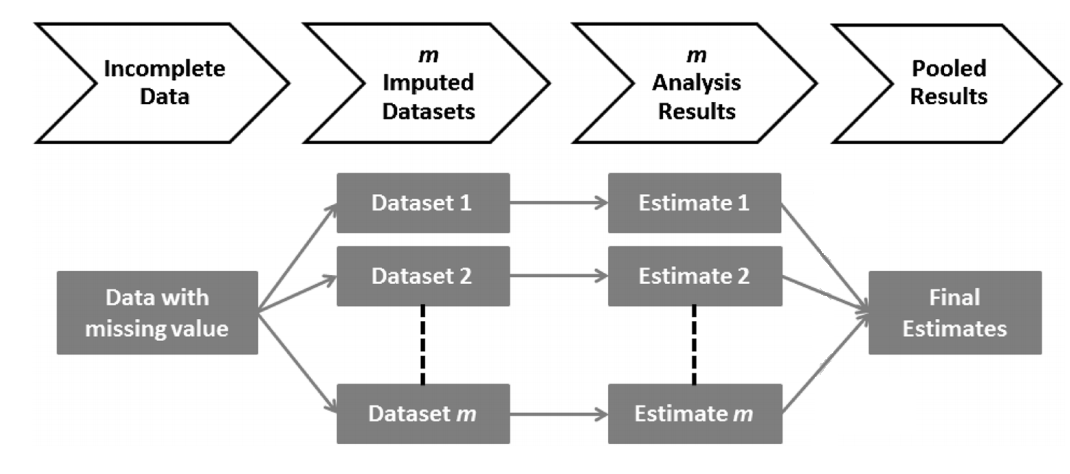
\includegraphics[width=\textwidth]{MultipleImputationPicture.PNG}
		\caption{An graphical layout of multiple imputation. At the start a dataset with missing values is present. Missing values are imputed $m$ times to create $m$ imputed datasets. The $m$ complete datasets are all analysed for $m$ different sets of estimates. These results are then pooled into one complete set of estimates. \cite{chevret2015multiple, rubin1976inference}}
		\label{fig:MultipleImputationLayout}
	\end{figure}
	
	
	\begin{itemize}
		
		\item \textit{Value imputation} \\
		Different approaches are available for the value imputation per dataset. One is similar to the previously discussed SI hot deck imputation. The quickest imputation would be to randomly choose a value from the distribution of the feature. After analysing all different datasets and combining them, it would seem as if the missing values were following the same distribution. Other techniques are similar to the multivariate regression imputation and the kNN imputation \cite{pedersen2017missing, white2011multiple}. The variance can be added manually. The variance is then averaged for all variances and in the end using a new averaged variance \cite{donders2006gentle}. Other mainly regression methods use different initial seeds as a way of creating a variance \cite{he2010multiple}.
		
		\item \textit{Additional datasets} \\
		The number of suggested datasets is different per study and usually differs between 3 and 10 \cite{van2007multiple, pedersen2017missing, van1999multiple, van2006imputation, azur2011multiple, royston2004multiple}, however outliers of 15 \cite{martin2018impact} and even 25 \cite{raghunathan2001multivariate} are known. Other researchers even propose the number of datasets to be the same as the percentage of missing values \cite{white2011multiple}. The number of datasets is proportionally to the quality of the result and more datasets would indicate a better result. However generating and analysing more datasets also takes much more computation time, therefore a trade-off in computation time and quality should be considered.
		
		\item \textit{Analysis} \\
		The analysis of the dataset is project specific. For example, if the outcome should be a linear equation between features and output, linear regression should be used to compute such an equation. Usually the outcome of such an analysis is more precise than it actually should be. By doing the same analysis multiple times with MuI, a measure of uncertainty can be given to the outcome. This is done by combining the different outcomes together to one final outcome, by for example show standard deviations per regression coefficient \cite{donders2006gentle, van2006imputation}.
		
	\end{itemize}	
	
	% Advantages and disadvantages
	The main advantage of multiple imputation is the addition of imputation uncertainty. In single imputation this uncertainty is unfairly low, which can create bias in results. Because of it being an extension on single imputation, it also inherits the advantages of being able to handle MAR values and possibly MNAR, and raises the number of samples to be used for analysis \cite{van2006imputation, pedersen2017missing}. The disadvantages mainly consist of taking up more computation time, due to multiplication of the analysis for the datasets. Therefore complex analysis techniques that take longer to compute may become unusable. Another aspect is the error given to missing value imputations. Not all analysis techniques perform well with errors which may create worse results even after combining the results \cite{pedersen2017missing}.
	
	% Implementations and MICE
	Several MuI implementations are created and also added to mainly statistical analysis programs as SOLAS, SAS, SPSS, S-Plus and Stata \cite{horton2001multiple, allison2000multiple, royston2011multiple}. The most used implementation is multiple imputation for chained equations (MICE) \cite{azur2011multiple, royston2004multiple}, also known as sequential regression multiple implementation (SRMI) \cite{he2010multiple}. MICE stores the location of the missing values and iteratively replaces them with new values, according to a six step system \cite{azur2011multiple}. 
	
	\begin{enumerate}
		\item Replace all missing values with the mean of the corresponding feature.
		\item Choose a feature $f$ and remove the imputed values on all missing value locations.
		\item Create a model with all samples that do not have a missing value in $f$ to predict the value in $f$ by the other features.
		\item Impute the values in $f$ using the created model.
		\item Repeat steps 2 to 4 for all features that have missing values.
		\item Iteratively repeat steps 2 to 5 $s$ cycles for better more precise imputed values to create a final dataset.
	\end{enumerate}
	
	% Continuation MICE implementation
	The six steps create one dataset. The steps are $m$ times with different orders of choosing $f$ to create $m$ different datasets for analysis. The number of cycles used in the sixth step influences the precision of the outcome, as eventually the imputed missing values are expected to converge to one value. Usually about 10 cycles are done, as it is a good equilibrium between low computation time and high imputed value precision \cite{azur2011multiple, royston2004multiple}.
	
	%\subsection{Outlier Detection}
	%\label{subsec:OutlierDetection}
	
	\section{Hypotheses}
	\label{MVsec:Hypothesis}
	
	The main goal for this chapter is to find more insight in quality enhancement and add that insight to the final framework. Several hypotheses are made before designing experiments to test them and are discussed here:
	
	\begin{enumerate}
		\item \textit{Distribution preservation} \\
		One thing missing value handling algorithms should do is preserve the distribution of a feature, not creating any bias in it. List Deletion methods CCA and ACA are not expected to do that properly in most cases, as most values are not MCAR. WCA might be able to efficiently tackle distribution problems, but is expected to be outperformed by imputation methods. Of the imputation methods MICE is expected to perform best, followed by kNN and regression imputation. Hot deck and mean imputation obviously are also expected to preserve distribution characteristics very well as their imputation method is based on it. \\
		\\
		\emph{H1: The advanced imputation methods (MICE, kNN and regression) are expected to preserve the distribution very well, much better than the list deletion methods. Hot deck and mean imputation should be able to preserve the distribution, too, as they use distribution characteristics in their imputation.}\\
		\\
		\item \textit{Quality improvement} \\
		Missing values handling algorithms are necessary, however can show different levels of quality improvement. This difference in quality shows the best approaches to cope with missing values. Again, list deletion algorithms are expected to perform worst in quality improvement. Next are the easy single imputation methods, the mean imputation, hot encoding and missing indicator algorithms. These are followed by the more advanced single imputation algorithms the kNN and regression algorithms. The multiple imputation algorithm MICE is expected to outperform all.\\
		\\
		\emph{H2: The advanced imputation methods (MICE, kNN and regression) are expected to improve quality the most, followed by the more simple imputation algorithms (means, missing indicator and hot deck). List deletion methods are expected to perform worst in quality improvement.}\\
		\\
	\end{enumerate}
	
	\section{Methods}
	\label{MVsec:Methods}
	
	% Introduction
	To determine the quality of different missing value handling algorithms, two different approaches are used. The first approach focuses on the distributions of the different features and whether the algorithms create a bias in feature distributions. The second approach focuses on the evaluation quality and which missing value handling algorithm works best on predicting output. The four example datasets (Subsection \ref{MVsubsec:Datasets}) were used as example datasets for the experiments.
	
	
	\subsection{Bias Evaluation}
	\label{MVsubsec:BiasEvaluation}
	
	% Introduction
	After manipulating a dataset, the distributions of a feature can change significantly. This change in distribution can create a bias in the results and must be prevented as much as possible. To find out whether this bias is present, feature type specific values are compared between both the old and new feature values and those are compared using several statistical methods.
	
	% Statistical distribution measurement methods
	For future mentions of the two distributions that are compared the names 'old data' (before list deletion or value imputation) and 'new data' (after list deletion or value imputation) are used. The statistical methods that are used to find bias are all based on the same hypothesis Hyp0: the old data and new data originate from the same distribution. This means the rejection hypothesis becomes Hyp1: old and new data do not originate from the same distribution. Since features were numeric, ordinal or categorical, every feature type hypothesis is evaluated differently:
	
	\begin{itemize}
		\item \textit{Numeric features} \\
		For numeric features the mean and variance are main aspects to compare numeric distributions. To either accept the hypothesis, these two aspects are tested. The mean comparisons were done by using the known t-test \cite{heiberger2004statistical}. Normality is not assumed, however the t-test does not show worse performance when the sample size is reasonable \cite{bartlett1935effect}, which is the case. The equality of variance is tested by using a Levene's test with the Brown and Forsythe adaptation. This variance test was chosen due to not having any major assumptions on the distributions, for example the normality distribution \cite{brown1974robust}.
		\item \textit{Ordinal features} \\
		For ordinal features the mean cannot be used, as values are either not numeric or only give an indication with the numeric values. Because of that the median is used instead. The hypothesis is tested by checking whether this median is the same for both the old and new values. To have a better look at the distribution of the ordinal values, also a chi square test is done. This chi square test computes whether the distribution of ordinal values is the same for both the old and new values \cite{satorra2001scaled}.
		\item \textit{Categorical features} \\
		Categorical features do not have a mean or median, due to no ordering being present. Therefore the mode of the old and the new distribution is checked to be the same, to test the hypothesis Hyp0 to be true. On top of that, the chi square test is here used, to find out whether the features from before and after the missing values algorithms can follow the same distribution \cite{satorra2001scaled}.
	\end{itemize}
	
	% Missing Value Handling Algorithms
	All features from the four datasets are tested whether any bias is present or not. The missing values are handled by seven different algorithms: CCA (Algorithm \ref{alg:CCA}), ACA (Algorithm \ref{alg:ACA}), Mean/Median/Mode imputation (Algorithm \ref{alg:MeanImputation}), Hot Deck imputation (Algorithm \ref{alg:HotDeckImputation}), kNN imputation (Algorithm \ref{alg:kNNImputation}), Regression imputation(Algorithm \ref{alg:RegressionImputation}) and at last MICE (Subsection \ref{MVsubsec:MissingValueHandling}). An overview of the datasets, evaluation tests and the missing value handling algorithms is provided (Table \ref{tab:BiasEvaluationTable}).
	
	\begin{table}[]
		\caption{The three different aspects of the bias evaluation. Four different datasets are used. Two tests are done per feature type, to test hypothesis Hyp0 and seven missing value handling algorithms are implemented to be tested.}
		\label{tab:BiasEvaluationTable}
		\begin{tabular}{l|l|l}
			\textbf{Datasets}   & \begin{tabular}[c]{@{}l@{}}Heart Attack dataset\\ Hepatitis dataset\\ Cirrhosis dataset\\ Cervical cancer dataset\end{tabular}                                      & \begin{tabular}[c]{@{}l@{}}All datasets containing missing values \\ that are evaluated\end{tabular}                                                                                        \\ \hline
			\textbf{Test types} & \begin{tabular}[c]{@{}l@{}}Numeric features (t-test, Levene's test)\\ Ordinal features  (median, chi-square)\\ Categorical features (mode, chi-square)\end{tabular} & \begin{tabular}[c]{@{}l@{}}Different types of features have different \\ tests for hypothesis Hyp0: The old and \\ new distributions are the same\end{tabular}                                \\ \hline
			\textbf{Methods}    & \begin{tabular}[c]{@{}l@{}}CCA\\ WCA\\ Mean/Median/Mode imputation\\ Hot deck imputation\\ kNN imputation\\ Regression imputation\\ MICE\end{tabular}               & \begin{tabular}[c]{@{}l@{}}All methods to handle missing values:\\ - Two List Deletion algorithms\\ - Four Single Imputation algorithms\\ - One Multiple Imputation algorithms\end{tabular}
		\end{tabular}
	\end{table}
	
	% Tables
	The outcome of all the tests are shown in multiple tables. In those tables tests that show a rejection of Hyp0 are highlighted. For the list deletion algorithms, additionally the type of missing values is evaluated by also testing the change in distribution in values without missing values. If a feature distribution changes for a feature without missing values after removing all missing values, a relation is present and the missing values are not MCAR. Aside from these tables plots of the relation between the percentage of missing values and probability of bias being present are made for every algorithm. This can indicate quality between the different algorithms with regards of the statistical hypothesis. In those plots also a regression line is shown with also the $R^2$ value, to show the quality of the regression \cite{draper2014applied}. An equation for $R^2$ is given for clarification (Equation \ref{eq:R2}). 
	
	\begin{equation}\label{eq:R2}
	R^2 = \frac{SS_{tot} - SS_{res}}{SS_{tot}}), SS_{tot} = \sum(y_i - \bar{y})^2, SS_{res} = \sum(y_i - f_i)^2 
	\end{equation} 
	
	$R^2$ is measured by first measuring the variance sum towards the mean ($SS_{tot}$, $y_i$ is the value for data point $i$, $\bar{y}$ is the mean of data points $y$) and the variance sum towards the regression line ($SS_{reg}$, $f_i$ is regression value for $i$). Secondly the difference is measured and this difference is normalized by dividing it by the mean variance sum. $R^2$ should be a value on interval $[0, 1]$ with $1$ being a good fit and $0$ being a bad fit.
	
	\subsection{Quality Evaluation}
	\label{MVsubsec:QualityEvaluation}
	
	To determine the quality of the missing value imputation methods, the classification quality of the dataset was tested after handling the missing values. This is done for the Hepatitis, Cirrhosis and Cervical Cancer datasets, as on the Heart Attack dataset regression should be performed. This classification quality was tested by using the basic logistic regression algorithm from \textit{scikit-learn}. This classification algorithm only accepts numerical data, therefore all categorical features are first hot encoded. Previously discussed missing value handling algorithms (Table \ref{tab:MethodsExplanation}) are tested on their accuracy, precision, recall and F1 score with a 10-fold cross validation. For the datasets an additional classification was done after removing the values with more than 15\% missing values, to find out if that would give a difference in quality, as well. 
	
	\begin{table}[H]
		\caption{All tested missing value handling methods and possible parameters used during testing}
		\label{tab:MethodsExplanation}
		\begin{tabular}{l|l|l}
			\textbf{Type}                & \multicolumn{1}{l|}{\textbf{Method}}                                          & \textbf{Parameters}                                                                \\ \hline
			\textbf{List Deletion}       & \begin{tabular}[c]{@{}l@{}}CCA\\ (Algorithm \ref{alg:CCA})\end{tabular}                 &                                                                                    \\ \cline{2-3}
			\textbf{}                    & \begin{tabular}[c]{@{}l@{}}ACA\\ (Algorithm \ref{alg:ACA})\end{tabular}                 & - threshold: 10\% missing values \\ \cline{2-3}
			\textbf{}                    & \begin{tabular}[c]{@{}l@{}}WCA\\ (Algorithm \ref{alg:WCA})\end{tabular}                 &                                                                                    \\ \hline
			\textbf{Single Imputation}   & \begin{tabular}[c]{@{}l@{}}Mean/Median/Mode\\ (Algorithm \ref{alg:MeanImputation})\end{tabular}    &                                                                                    \\ \cline{2-3}
			\textbf{}                    & \begin{tabular}[c]{@{}l@{}}Hot deck\\ (Algorithm \ref{alg:HotDeckImputation})\end{tabular}            &                                                                                    \\ \cline{2-3}
			\textbf{}                    & \begin{tabular}[c]{@{}l@{}}Missing indicator\\ (Algorithm \ref{alg:MissingIndicatorImputation})\end{tabular}   &  - Imputed value: Mean, 0     \\ \cline{2-3}
			\textbf{}                    & \begin{tabular}[c]{@{}l@{}}Regression\\ (Algorithm \ref{alg:RegressionImputation})\end{tabular}          &                                                                                    \\ \cline{2-3}
			\textbf{}                    & \begin{tabular}[c]{@{}l@{}}k-Nearest neighbour\\ (Algorithm \ref{alg:kNNImputation})\end{tabular} & - k =  1, 3, 5                        \\ \hline
			\textbf{Multiple Imputation} & \begin{tabular}[c]{@{}l@{}}MICE\\ (Subsection \ref{MVsubsec:MissingValueHandling})\end{tabular}                & \begin{tabular}[c]{@{}l@{}}s = 3, 5\\ m = 3, 5\end{tabular}                       
		\end{tabular}
	\end{table}
	
	% Datasets tables
	To show the differences between the datasets, the best outcomes are shown separately, as well as an average over the three datasets. This way interesting differences between the datasets can be located and discussed. 
	
	\section{Results}
	\label{MVsec:Results}
	
	\subsection{Bias Evaluation Results}
	\label{MVsubsec:BiasEvaluationResults}
	
	% Tables in appendix
	The outcome of the distribution tests for the heart attack dataset are shown (Tables \ref{tab:LDHeartAttack} and \ref{tab:ImputationHeartAttack}), as well as the tables for the other datasets (Appendix \ref{app:DistributionTables}). The tables are split between list deletion (Table \ref{tab:LDHeartAttack}) and imputation (Table \ref{tab:ImputationHeartAttack}) results.
	
	\begin{table}[H]
		\caption{Testing for the heart attack data set whether the type of missing values can be represented by the remaining values. This is done by comparing distributions between the old and new data after CCA and WCA. For numeric values, two tests were used, an independent t-test for equality of mean and a Levene's test with the median in brackets to test equality of variance. For ordinal and categorical features the medians and modes where compared respectively as well as a chi squared test in brackets for equality of distribution. P-values lower than $p < 0.05$ are marked red for failure of representation, p-values higher than $p > 0.05$ are marked green for correctly being represented. If at least one feature is not represented after CCA, the missing values cannot be MCAR. If at least one feature is not represented after WCA, the pseudo-randomness cannot be corrected by only using weights for other values.}
		\label{tab:LDHeartAttack}
		\begin{tabular}{l|lll|lll|lll}
			\textbf{\begin{tabular}[c]{@{}l@{}}Feature \\ name\end{tabular}} & \textbf{\begin{tabular}[c]{@{}l@{}}still\\ alive\end{tabular}} & \textbf{age}                                                                             & \textbf{\begin{tabular}[c]{@{}l@{}}peri-\\ cardial\end{tabular}} & \textbf{\begin{tabular}[c]{@{}l@{}}frac-\\ tional\end{tabular}}                          & \textbf{epss}                                                                 & \textbf{lvdd}                                                                 & \textbf{\begin{tabular}[c]{@{}l@{}}wall\\ score\end{tabular}}                            & \textbf{\begin{tabular}[c]{@{}l@{}}wall\\ index\end{tabular}}                 & \textbf{\begin{tabular}[c]{@{}l@{}}alive\\ at 1\end{tabular}} \\ \hline
			\textbf{\begin{tabular}[c]{@{}l@{}}Value \\ type\end{tabular}}   & Cat                                                            & Num                                                                                     & Cat                                                              & Num                                                                                     & Num                                                                          & Num                                                                          & Num                                                                                     & Num                                                                          & Cat                                                           \\ \hline
			\textbf{Missing (\%)}   & 0\%                                                            & 3.85\%                                                                                   & 0\%                                                              & 5.38\%                                                                                   & 10.77\%                                                                       & 7.69\%                                                                        & 2.31\%                                                                                   & 0.77\%                                                                        & 43.85\%                                                       \\ \hline
			\textbf{\begin{tabular}[c]{@{}l@{}}p-values \\ CCA\end{tabular}} & \cellcolor[HTML]{009901}\begin{tabular}[c]{@{}l@{}}True\\ (0.96)\end{tabular}                        & \cellcolor[HTML]{9A0000}\begin{tabular}[c]{@{}l@{}}\textless{}0.01\\ (0.39)\end{tabular} & \cellcolor[HTML]{009901}\begin{tabular}[c]{@{}l@{}}True\\ (0.99)\end{tabular}                          & \cellcolor[HTML]{9A0000}\begin{tabular}[c]{@{}l@{}}\textless{}0.01\\ (0.83)\end{tabular} & \cellcolor[HTML]{009901}\begin{tabular}[c]{@{}l@{}}0.99\\ (0.74)\end{tabular} & \cellcolor[HTML]{009901}\begin{tabular}[c]{@{}l@{}}0.99\\ (0.94)\end{tabular} & \cellcolor[HTML]{9A0000}\begin{tabular}[c]{@{}l@{}}\textless{}0.01\\ (0.98)\end{tabular} & \cellcolor[HTML]{009901}\begin{tabular}[c]{@{}l@{}}0.09\\ (0.84)\end{tabular} & \cellcolor[HTML]{009901}\begin{tabular}[c]{@{}l@{}}True\\ (0.94)\end{tabular}                                  \\
			\textbf{\begin{tabular}[c]{@{}l@{}}p-values\\ WCA\end{tabular}}  & \cellcolor[HTML]{009901}\begin{tabular}[c]{@{}l@{}}True\\ (1.00)\end{tabular}                                  & \cellcolor[HTML]{009901}\begin{tabular}[c]{@{}l@{}}0.48\\ (0.82)\end{tabular}            & \cellcolor[HTML]{009901}\begin{tabular}[c]{@{}l@{}}True\\ (0.98)\end{tabular}                         & \cellcolor[HTML]{9A0000}\begin{tabular}[c]{@{}l@{}}\textless{}0.01\\ (0.45)\end{tabular} & \cellcolor[HTML]{009901}\begin{tabular}[c]{@{}l@{}}0.99\\ (0.39)\end{tabular} & \cellcolor[HTML]{009901}\begin{tabular}[c]{@{}l@{}}0.99\\ (0.28)\end{tabular} & \cellcolor[HTML]{9A0000}\begin{tabular}[c]{@{}l@{}}\textless{}0.01\\ (0.54)\end{tabular} & \cellcolor[HTML]{009901}\begin{tabular}[c]{@{}l@{}}0.99\\ (0.91)\end{tabular} & \cellcolor[HTML]{009901}\begin{tabular}[c]{@{}l@{}}True\\ (0.92)\end{tabular}                      
		\end{tabular}
	\end{table}
	
	% Observations in tables
	The tables show that in the heart attack, cirrhosis and cervical cancer datasets at least one feature shows a difference between the old and new data. Highlights are shown for changes in distribution for all values:
	
	\begin{itemize}
		\item \textit{Heart attack} \\ 
		\textit{age}, \textit{fractional} and \textit{wall score} all have $p < 0.01$ for having the same mean before and after CCA. This indicates that the missing value type of at least one feature is MAR and for all three possibly even MNAR. WCA does help in creating a representative distribution for the feature \textit{age}, however \textit{fractional} and \textit{wall score} still are differently distributed. Other approaches to handle missing values are most likely more effective
		\item \textit{Hepatitis} \\ 
		For no feature a reason to reject the distributions before and after deleting samples with missing values is present. The feature that is least likely to have the same distribution is \textit{bilirubin} with having a $p = 0.14$ for the same mean and $p = 0.23$ for the same variance. We therefore cannot say that the missing values are MCAR and using only CCA to handle missing values is certainly possible. WCA has worse results for several features and show that WCA might not be the best way to improve the sample size for this dataset.
		\item \textit{Cirrhosis} \\ 
		\textit{case number}, \textit{status}, \textit{day}, \textit{albumin} and \textit{SGOT} all have $p < 0.05$ if numeric for having the same mean and \textit{False} if ordinal or categorical for having the same median or mode, respectively. These five features do not have missing values. This means that the bias in the distribution is caused by list deletion due to another feature's missing values. Therefore it can be concluded that at least for one feature the missing values are at least MAR. WCA helps fixing the distributions for \textit{case number} and \textit{SGOT}, but also creates additional bias in \textit{presence of ascites}, \textit{presence of hepatocytes} and \textit{presence of edema} and therefore is not a suitable approach to remove possible bias. 
		\item \textit{Cervical cancer} \\ 
		\textit{STDs}, \textit{\#STDs}, \textit{condylomatosis}, \textit{vulvoperineal condylomatosis} and \textit{STDs \#diagnosis} all have $p < 0.05$ if numeric for having the same mean and \textit{False} if categorical for having the same mode. All but \textit{STDs \#diagnosis} also have a $p < 0.05$ for having the same variance if numeric or the same chi square distribution if categorical, which further strengthens hypothesis H1 of the distributions being different. This indicates that the missing values of at least one feature is MCAR.
	\end{itemize}
	
	\begin{table}[h!]
		\caption{A table showing the number of samples that remained after performing CCA.}
		\label{tab:CCARemainingSamples}
		\begin{tabular}{l|l|l}
			\textbf{Dataset}      & \textbf{Total samples} & \textbf{\begin{tabular}[c]{@{}l@{}}Number of samples \\ after CCA\end{tabular}} \\ \hline
			\textbf{Heart Attack} & 108                    & 61                                                                                \\
			\textbf{Hepatitis}    & 155                    & 80                                                                                \\ \hline
			\textbf{Cirrhosis }            & 1945                   & 1113                                                                              \\
			\textbf{Cervical Cancer}       & 585                    & 59                                                                               
		\end{tabular}
	\end{table}
	
	The heart attack, cirrhosis and cervical cancer datasets all indicate possible bias after deleting samples with missing values. On top of that, after removing all samples with missing values not many samples are left for any of the datasets (Table \ref{tab:CCARemainingSamples}). The hepatitis dataset loses almost 50\% of its samples after CCA and the cervical cancer dataset drops down to only 10\% of its original values. All four datasets would therefore potentially benefit from an imputation approach.
	
	\begin{table}[]
		\caption{Testing for the heart attack data set if certain types of imputation create a vastly different distribution for features with missing values. The imputation values are generated with mean imputation, hot deck imputation, k-Nearest Neighbour imputation ($k = 3$), regression imputation and MICE (number of cycles is $s = 5$). For numeric values, two tests were used, an independent t-test for equality of mean and a Levene's test with the median in brackets to test equality of variance. For ordinal and categorical features the medians and modes where checked respectively to be similar as well as a chi squared test in brackets fro equality of distribution. P-values lower than $p < 0.05$ are marked red for failure of representation, p-values close to $p > 0.05$ are marked green for correctly being represented.}
		\label{tab:ImputationHeartAttack}
		\begin{tabular}{l|ll|lll|ll}
			\textbf{\begin{tabular}[c]{@{}l@{}}Feature \\ name\end{tabular}}         & \textbf{age}                                                                  & \textbf{\begin{tabular}[c]{@{}l@{}}frac-\\ tional\end{tabular}}               & \textbf{epss}                                                                 & \textbf{lvdd}                                                                 & \textbf{\begin{tabular}[c]{@{}l@{}}wall\\ score\end{tabular}}                 & \textbf{\begin{tabular}[c]{@{}l@{}}wall\\ index\end{tabular}}                 & \textbf{\begin{tabular}[c]{@{}l@{}}alive\\ at 1\end{tabular}} \\ \hline
			\textbf{\begin{tabular}[c]{@{}l@{}}Value \\ type\end{tabular}}           & Num                                                                          & Num                                                                          & Num                                                                          & Num                                                                          & Num                                                                          & Num                                                                          & Cat                                                           \\
			\textbf{Missing}          & 3.85\%                                                                        & 5.38\%                                                                        & 10.77\%                                                                       & 7.69\%                                                                        & 2.31\%                                                                        & 0.77\%                                                                        & 43.85\%                                                       \\ \hline
			\textbf{\begin{tabular}[c]{@{}l@{}}Mean\\ Imputation\end{tabular}}       & \cellcolor[HTML]{009901}\begin{tabular}[c]{@{}l@{}}1.00\\ (0.76)\end{tabular} & \cellcolor[HTML]{009901}\begin{tabular}[c]{@{}l@{}}0.99\\ (0.60)\end{tabular} & \cellcolor[HTML]{009901}\begin{tabular}[c]{@{}l@{}}0.99\\ (0.39)\end{tabular} & \cellcolor[HTML]{009901}\begin{tabular}[c]{@{}l@{}}1.00\\ (0.48)\end{tabular} & \cellcolor[HTML]{009901}\begin{tabular}[c]{@{}l@{}}1.00\\ (0.88)\end{tabular} & \cellcolor[HTML]{009901}\begin{tabular}[c]{@{}l@{}}1.00\\ (0.98)\end{tabular} & \cellcolor[HTML]{009901}\begin{tabular}[c]{@{}l@{}}True\\ (0.77)\end{tabular}                      \\
			\textbf{\begin{tabular}[c]{@{}l@{}}Hot Deck\\ Imputation\end{tabular}}   & \cellcolor[HTML]{009901}\begin{tabular}[c]{@{}l@{}}0.97\\ (0.98)\end{tabular} & \cellcolor[HTML]{009901}\begin{tabular}[c]{@{}l@{}}0.88\\ (0.88)\end{tabular} & \cellcolor[HTML]{009901}\begin{tabular}[c]{@{}l@{}}0.94\\ (0.98)\end{tabular} & \cellcolor[HTML]{009901}\begin{tabular}[c]{@{}l@{}}0.82\\ (0.91)\end{tabular} & \cellcolor[HTML]{009901}\begin{tabular}[c]{@{}l@{}}0.94\\ (0.86)\end{tabular} & \cellcolor[HTML]{009901}\begin{tabular}[c]{@{}l@{}}0.96\\ (0.96)\end{tabular} & \cellcolor[HTML]{009901}\begin{tabular}[c]{@{}l@{}}True\\ ( 0.96)\end{tabular}                      \\ \hline
			\textbf{\begin{tabular}[c]{@{}l@{}}kNN\\ Imputation\end{tabular}}        & \cellcolor[HTML]{009901}\begin{tabular}[c]{@{}l@{}}0.86\\ (0.99)\end{tabular} & \cellcolor[HTML]{009901}\begin{tabular}[c]{@{}l@{}}0.81\\ (0.88)\end{tabular} & \cellcolor[HTML]{009901}\begin{tabular}[c]{@{}l@{}}0.69\\ (0.62)\end{tabular} & \cellcolor[HTML]{009901}\begin{tabular}[c]{@{}l@{}}0.94\\ (0.68)\end{tabular} & \cellcolor[HTML]{009901}\begin{tabular}[c]{@{}l@{}}0.96\\ (0.97)\end{tabular} & \cellcolor[HTML]{009901}\begin{tabular}[c]{@{}l@{}}0.96\\ (0.98)\end{tabular} & \cellcolor[HTML]{009901}\begin{tabular}[c]{@{}l@{}}True\\ (0.91)\end{tabular}                       \\
			\textbf{\begin{tabular}[c]{@{}l@{}}Regression\\ Imputation\end{tabular}} & \cellcolor[HTML]{009901}\begin{tabular}[c]{@{}l@{}}0.84\\ (1.00)\end{tabular} & \cellcolor[HTML]{009901}\begin{tabular}[c]{@{}l@{}}0.71\\ (0.95)\end{tabular} & \cellcolor[HTML]{009901}\begin{tabular}[c]{@{}l@{}}0.34\\ (0.57)\end{tabular} & \cellcolor[HTML]{009901}\begin{tabular}[c]{@{}l@{}}0.91\\ (0.76)\end{tabular} & \cellcolor[HTML]{009901}\begin{tabular}[c]{@{}l@{}}0.88\\ (1.00)\end{tabular} & \cellcolor[HTML]{009901}\begin{tabular}[c]{@{}l@{}}0.93\\ (0.98)\end{tabular} & \cellcolor[HTML]{009901}\begin{tabular}[c]{@{}l@{}}True\\ (0.92)\end{tabular}                       \\ \hline
			\textbf{\begin{tabular}[c]{@{}l@{}}MICE\\ (5 cycles)\end{tabular}}       & \cellcolor[HTML]{009901}\begin{tabular}[c]{@{}l@{}}0.97\\ (0.81)\end{tabular} & \cellcolor[HTML]{009901}\begin{tabular}[c]{@{}l@{}}0.94\\ (0.80)\end{tabular} & \cellcolor[HTML]{009901}\begin{tabular}[c]{@{}l@{}}0.98\\ (0.90)\end{tabular} & \cellcolor[HTML]{009901}\begin{tabular}[c]{@{}l@{}}0.80\\ (0.84)\end{tabular} & \cellcolor[HTML]{009901}\begin{tabular}[c]{@{}l@{}}0.98\\ (0.98)\end{tabular} & \cellcolor[HTML]{009901}\begin{tabular}[c]{@{}l@{}}0.96\\ (0.97)\end{tabular} & \cellcolor[HTML]{009901}\begin{tabular}[c]{@{}l@{}}True\\ (0.93)\end{tabular}                      
		\end{tabular}
	\end{table}
	
	% Imputation methods
	Most imputation methods show an improvement in results. The heart attack dataset has no bias in distributions after any of the five tested imputation methods, the hepatitis dataset only has bias when using mean imputation or MICE, the cirrhosis dataset only shows bias when using mean imputation and at last in the cervical cancer dataset all but the two features with 91.75\% missing values contain no bias between distributions. On top of that, the only features that had bias in the newly created distributions are features with more than 40\% missing values, indicating that imputation methods have more problems when a higher missing/not missing ratio is present. This gives an indication that removal of features with missing values higher than 40\% would greatly help the usefulness of a dataset.
	
	% Plotting imputation methods
	A scatter plot with fitted linear curves is made to show a relation between the probability of the old and new mean (Figure \ref{fig:PMeanFits}) and variance (Figure \ref{fig:PVarianceFits}) originating from the same distribution and the percentage of values missing. Although the $R^2$ values for some of the regression lines seem plausible, the value distribution does not seem to support this. Most features are within the first 15\% of the missing values and the features above 15\% missing values seem to deviate significantly from the others.
	
	\begin{figure}[]
		\centering
		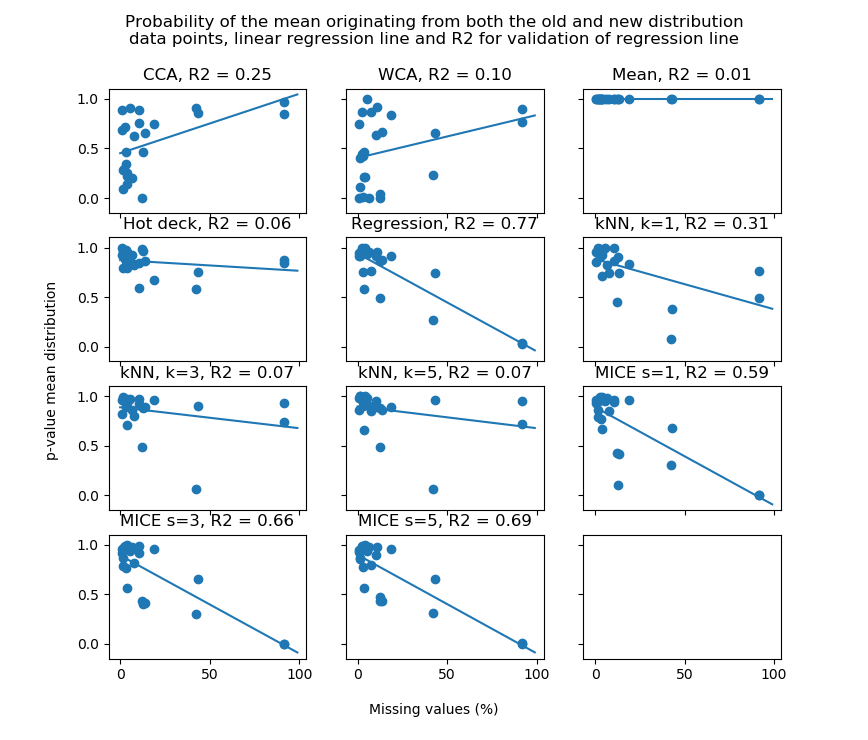
\includegraphics[width=\textwidth]{Mean_Dist.PNG}
		\caption{Plots showing the probability of bias being present in feature distributions. The mean of the features with the old distribution with missing values and the new distribution after missing value handling are compared and the p-value of them both originating from the same distribution is computed. Every feature of every dataset is a data point. On the x-axis the percentage of missing values is given for a feature and on the y-axis the p-value of the probability. For every missing value algorithm also a linear fit is made to show the trend of the scatter plot.}
		\label{fig:PMeanFits}
	\end{figure}
	
	\begin{figure}[]
		\centering
		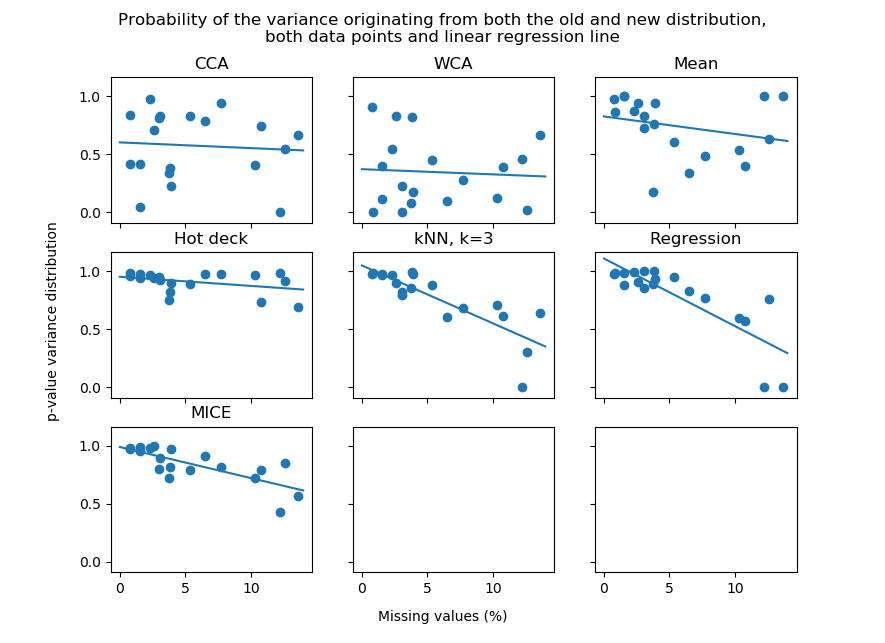
\includegraphics[width=\textwidth]{Var_Dist.PNG}
		\caption{Plots showing the probability of bias being present in feature distributions. The variance of the features with the old distribution with missing values and the new distribution after missing value handling are compared and the p-value of them both originating from the same distribution is computed. Every feature of every dataset is a data point. On the x-axis the percentage of missing values is given for a feature and on the y-axis the p-value of the probability. For every missing value algorithm also a linear fit is made to show the trend of the scatter plot.}
		\label{fig:PVarianceFits}
	\end{figure}
	
	It seems that it is difficult to perform imputation on features with more than 15\% missing values. Therefore an additional approach was used, by first performing ACA for features with more than 15\% missing values, followed by the known missing value handling techniques (Figure \ref{fig:PMeanFitsACA} and \ref{fig:PVarianceFitsACA}). 
	
	\begin{figure}[]
		\centering
		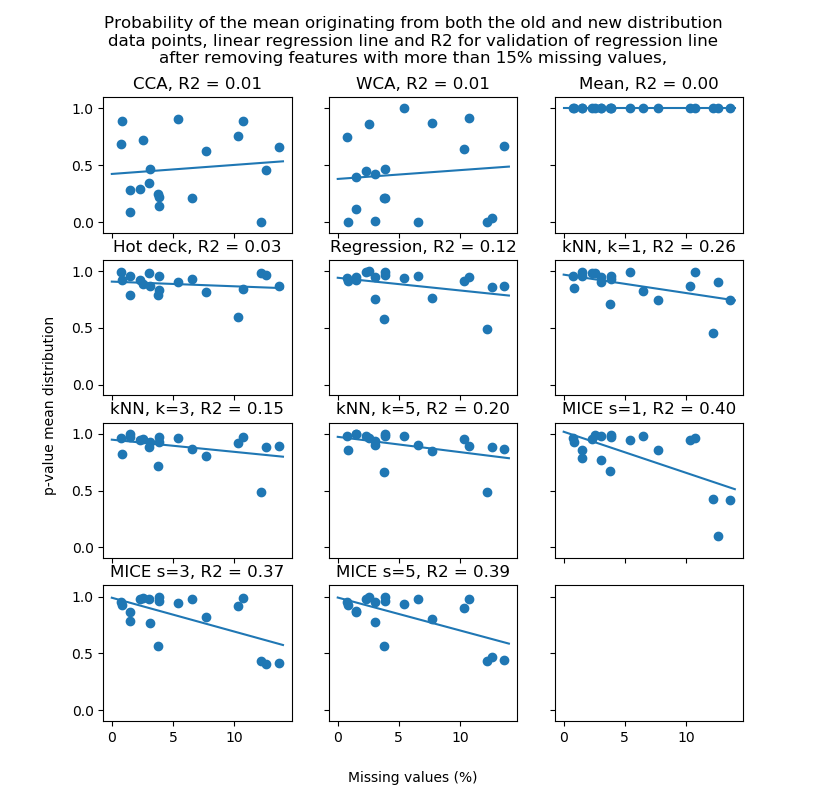
\includegraphics[width=\textwidth]{Mean_Dist_Extra_ACA.PNG}
		\caption{Plots showing the probability of bias being present in feature distributions. The mean of the features with the old distribution with missing values and the new distribution after missing value handling are compared and the p-value of them both originating from the same distribution is computed. Every feature of every dataset is a data point, however features with more than 15\% missing values are removed. On the x-axis the percentage of missing values is given for a feature and on the y-axis the p-value of the probability. For every missing value algorithm also a linear fit is made to show the trend of the scatter plot.}
		\label{fig:PMeanFitsACA}
	\end{figure}
	
	\begin{figure}[]
		\centering
		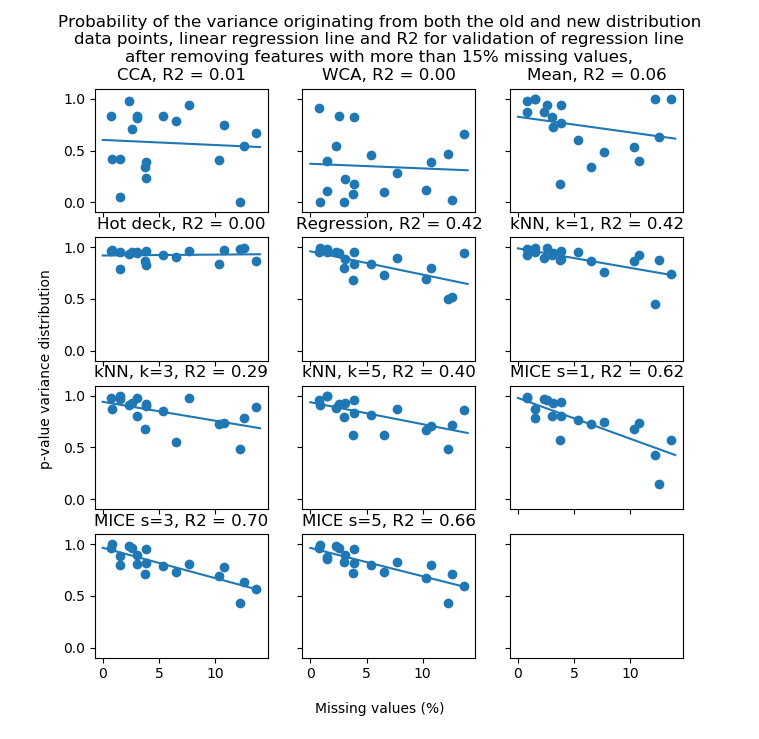
\includegraphics[width=\textwidth]{Var_Dist_Extra_ACA.PNG}
		\caption{Plots showing the probability of bias being present in feature distributions. The variance of the features with the old distribution with missing values and the new distribution after missing value handling are compared and the p-value of them both originating from the same distribution is computed. Every feature of every dataset is a data point, however features with more than 15\% missing values are removed. On the x-axis the percentage of missing values is given for a feature and on the y-axis the p-value of the probability. For every missing value algorithm also a linear fit is made to show the trend of the scatter plot.}
		\label{fig:PVarianceFitsACA}
	\end{figure}
	
	% List deletion
	List Deletion algorithms seem to be better at creating a representative distribution when more missing values are present. This is explainable for these datasets as all of them have a at least one feature with more than 40\%. Most samples are removed because of this feature also removing significant portions of other features. This results in features having more missing values will leave them with a higher percentage of their original values, therefore being closer to the original values.
	
	% Imputation
	The imputation algorithm seem to show big differences between the results. Hot deck imputation seems to create the best representative distribution, being the best when comparing mean and variance for the old and new distribution. Mean Imputation obviously shows a perfect fit for comparing means, however for variance imputation it is worse than both hot deck, kNN and regression. kNN imputation gave the best result after hot deck imputation. Interestingly kNN with k=1 neighbours shows the p-values for variance whereas k=3 and k=5 show the best p-values for the mean. Regression imputation shows good results as well, but is overall worse than kNN. MICE unexpectedly performs worse than regression and kNN in both mean and variance, even though it was expected to perform better.
	
	% Regression lines
	The regression lines for all imputations seem reasonable in performance. Either the p-value is almost independent of the percentage missing values (mean, hot deck, regression, kNN) or the $R^2 \approx 0.5$, showing somewhat of a trend in the data. Interestingly the p-value seems to deviate much more for higher percentages, something that is to be expected since the distribution can also change more when more values are missing.  
	
	% Explanation quality mean and hot deck
	The high quality for both mean and hot deck imputation can be explained by the evaluation methods. A mean comparison for mean imputation is obviously perfect, and the variance will always become smaller when more means are imputed. Hot deck imputation adds values according to the distribution of the features. This distribution follows the mean and variance of the original values and therefore the mean and variance will always be close to the original distribution. When looking at other aspects, for example the ability to predict the output with the dataset, hot deck imputation and mean imputation should show worse results as distribution specific estimations were imputed, instead of sample specific.
	
	\subsection{Quality Evaluation}
	\label{MVsubsec:QualityEvaluationResults}
	
	% Introduction
	The average results of the classification after using the missing value handling algorithms (Table \ref{tab:MethodsExplanation}) are shown in several figures. The average accuracy is shown for all three datasets without (Figure \ref{fig:EvalAvgAcc}) and with (Figure \ref{fig:EvalAvgAccExtraACA}) the removal of features with more than 15\% missing values  and without. The F1-score is also shown for the averaged dataset (Figure \ref{fig:EvalAvgF1}). At last a table to show the accuracy and F1 score is shown when all features with missing values are deleted to detect improvement for missing value imputation, as well as the best missing values handling algorithm for comparison (Table \ref{tab:ClassResults}).
	
	\begin{figure}[H]
		\centering
		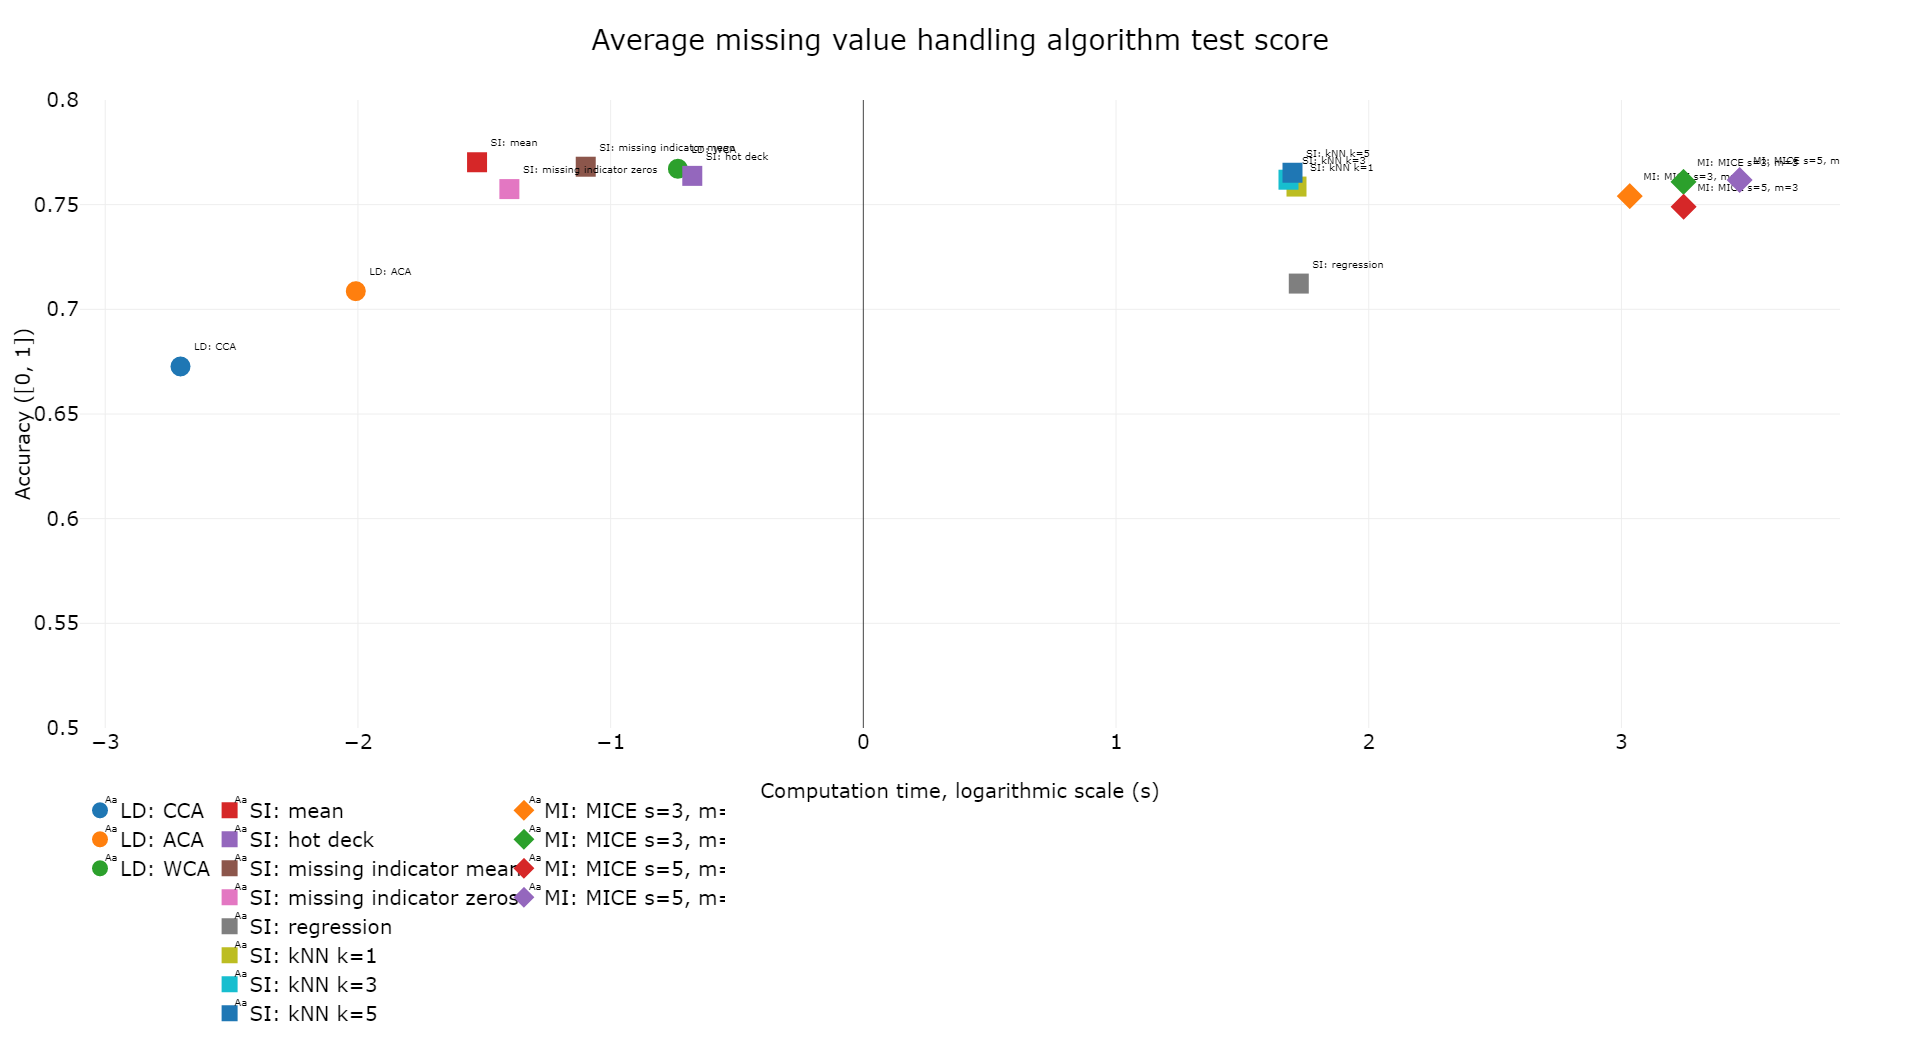
\includegraphics[angle=90,height=0.9\textheight]{avg_acc.PNG}
		\caption{A plot showing the average accuracy for the datasets classified after using a missing value handling algorithm. The x-axis shows the computation time for the missing values, done on a 10-logarithmic scale due to the big differences between them. The y-axis shows the accuracy on a scale of 0 to 1. The explanation of every data point can be found both in the text on the top right of the data point as well as in the legend.}
		\label{fig:EvalAvgAcc}
	\end{figure}
	
	\begin{figure}[H]
		\centering
		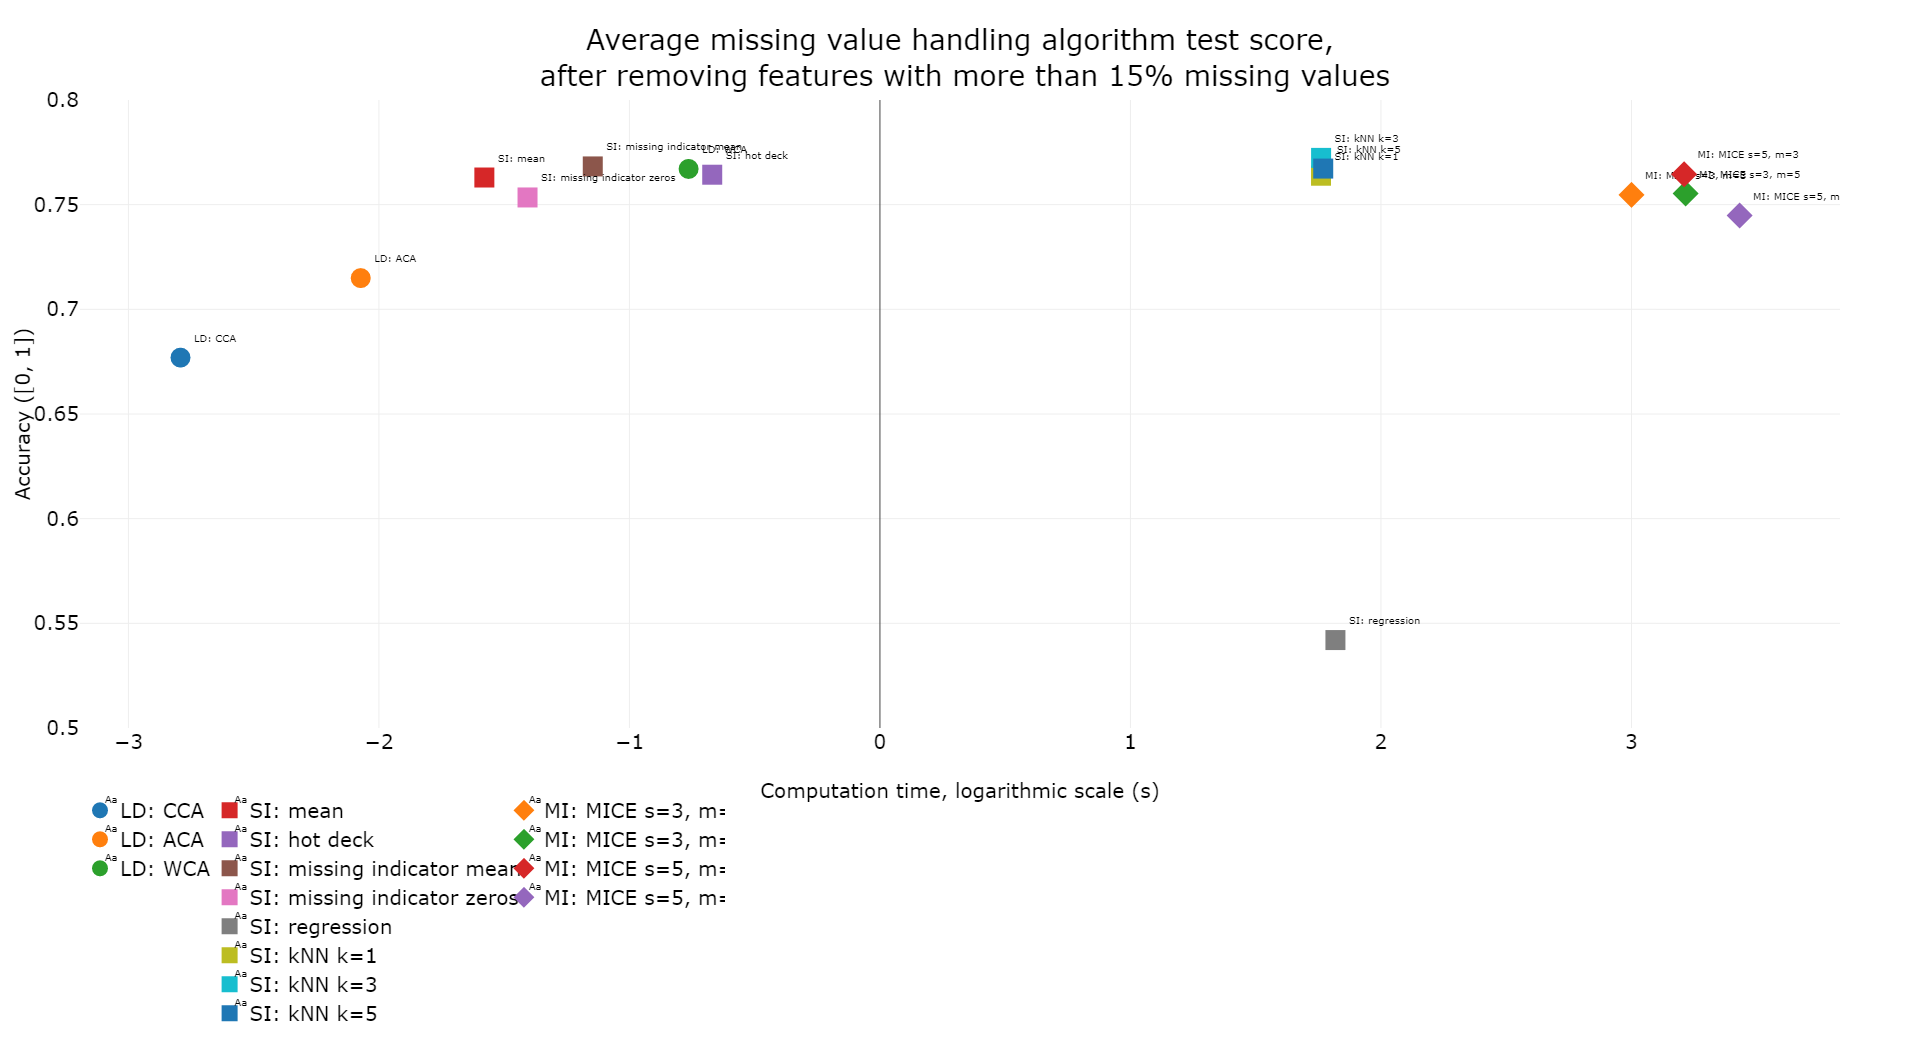
\includegraphics[angle=90,height=0.9\textheight]{avg_acc_15aca.PNG}
		\caption{A plot showing the average accuracy for the datasets classified after using a missing value handling algorithm and after removing all features with more than 15\% missing values. The x-axis shows the computation time for the missing values, done on a 10-logarithmic scale due to the big differences between them. The y-axis shows the accuracy on a scale of 0 to 1. The explanation of every data point can be found both in the text on the top right of the data point as well as in the legend.}
		\label{fig:EvalAvgAccExtraACA}
	\end{figure}
	
	\begin{figure}[H]
		\centering
		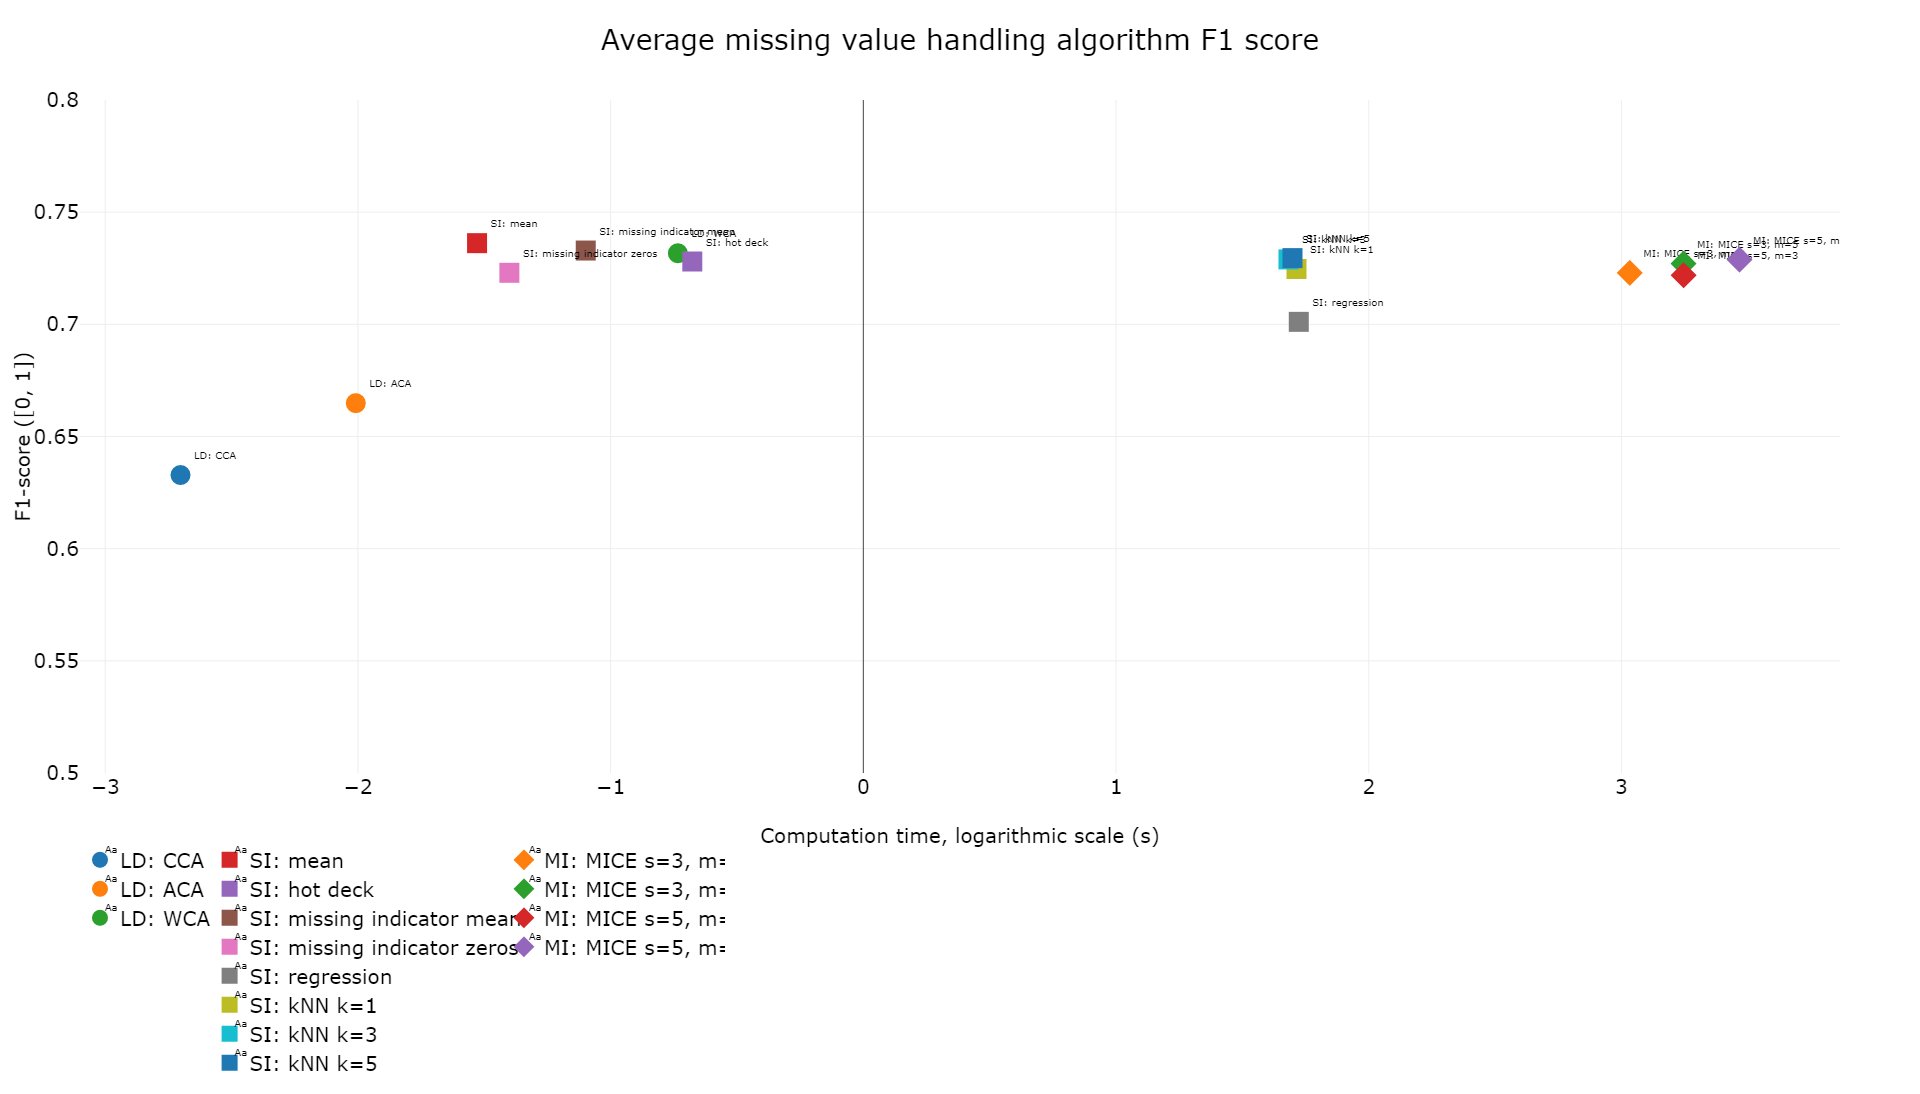
\includegraphics[angle=90,height=0.9\textheight]{avg_F1.PNG}
		\caption{A plot showing the F1-score for the datasets classified after using a missing value handling algorithm. The x-axis shows the computation time for the missing values, done on a 10-logarithmic scale due to the big differences between them. The y-axis shows the accuracy on a scale of 0 to 1. The explanation of every data point can be found both in the text on the top right of the data point as well as in the legend.}
		\label{fig:EvalAvgF1}
	\end{figure}
	
	
	\begin{table}[]
		\caption{The classification results of the datasets and the average after removing all features with missing values, as well as the best results after handling missing values.}
		\label{tab:ClassResults}
		\begin{tabular}{l|ll|lll}
			& \multicolumn{2}{l|}{\textbf{Without missing values}} & \multicolumn{3}{l}{\textbf{Best classification}}                                                                                                       \\
			\textbf{Dataset} & \textbf{Accuracy}         & \textbf{F1-score}        & \textbf{Accuracy} & \textbf{F1-score} & \textbf{Algorithm}                                                                                             \\ \hline
			Hepatitis        & 0.79                      & 0.75                     & 0.87              & 0.86              & Mean imputation                                                                                                \\
			Cirrhosis        & 0.56                      & 0.50                     & 0.57              & 0.52              & \begin{tabular}[c]{@{}l@{}}--\\
				1. CCA\\ 2. Missing indicator mean\\ 3. Missing indicator zeros\\ --\end{tabular} \\
			Cervical         & 0.74                      & 0.64                     & 0.89              & 0.83              & Mean imputation                                                                                                \\ \hline
			Average          & 0.70                      & 0.63                     & 0.77              & 0.74              & Mean imputation                                                                                               
		\end{tabular}
	\end{table}
	
	% Interpretation accuracy
	The values of the F1 score (Figure \ref{fig:EvalAvgF1}) are lower than the accuracy (Figure \ref{fig:EvalAvgAcc}), therefore the F1 score is also used in comparisons. The lack of difference in the accuracy in classification with (Figure \ref{fig:EvalAvgAccExtraACA}) and without features with more than 15\% missing values (Figure \ref{fig:EvalAvgAcc}), shows the lack of contribution of these values in the classification. Even though the distribution of the features improves (Subsection \ref{MVsubsec:BiasEvaluationResults}), the classification does not show any difference. This was not the case for the dataset with regression imputation, though, as the accuracy severely dropped after removing features with more than 15\% missing values from $0.72$ to $0.54$. Apparently important information was removed for the regression imputation to be successful.  
	
	% Separate methods
	When looking at separate methods, the difference in computation time can immediately be seen. List deletion algorithms and mean, missing indicator and hot deck single imputation algorithms all are very fast (less than a second), followed by k-nearest neighbour and regression single imputation (between 10 and 100 seconds) and at last multiple imputation methods (more than 1000 seconds). All imputation methods and WCA give the best accuracy, with little difference among them. The imputation methods and WCA all show an improvement compared with the accuracy when using only features without missing values (Table \ref{tab:ClassResults}), therefore using features with missing values does improve accuracy. The size of improvement differs per dataset, though, as the improvement for the Cervical dataset is 10 times higher than the improvement of the Cirrhosis dataset. 
	
	% Separate datasets
	Since the accuracy and F1-score of the datasets are significantly different (Table \ref{tab:ClassResults}), the results are also plotted per dataset separately (Appendix \ref{app:ClassPlots}). The low accuracy for regression imputation seems to originate mainly for the Cervical Cancer dataset. This can be a result of features in the Cervical Cancer dataset mostly consisting of boolean values. Hot encoded boolean values contain less information for regression, making it harder to find good imputation values. 
	
	% Best method
	The imputation methods show some differences in classification quality when looking at the results for the datasets separately. The Cirrhosis dataset shows hardly any improvement after using missing value handling algorithms, but its best results are when using a missing indicator method. The Hepatitis dataset result on the other hand is significantly worse when using the missing indicator method. This is supported by the bias evaluation (Subsection \ref{MVsubsec:BiasEvaluationResults}) and the dataset description (Subsection \ref{MVsubsec:Datasets}), as both showed that data in the Cirrhosis is confirmed MAR, whereas the data in the Hepatitis dataset was least likely to be MAR. This means that when data is very likely to be MAR, missing indicator value is more likely to be beneficial to the outcome. Aside from that, the kNN, regression and MICE imputation methods seem not worth the additional computation time for these datasets, even though in theory these methods make a more detailed guess of the outcome. 
	
	\section{Discussion}
	\label{MVsec:Discussion}
	
	% Research relevance
	Multiple studies have been performed to analyse missing value handling \cite{donders2006gentle, haukoos2007advanced, patrician2002multiple, sterne2009multiple, pedersen2017missing, raghunathan2001multivariate}. Most of these focus on complex imputation methods in cases for which imputation is very important. For initial analyses however, less complex methods help more in understanding what should be done and are therefore the basis of further investigation. Therefore, this research is more focused on imputation methods that are easier to understand and more simple to use.
	
	% Datasets
	The datasets used in these experiments are datasets with actual missing values. Whether the features with missing values are important for predicting the output however is unknown. Therefore the usefulness of either list deletion or imputation is unknown, too. This is visible in the difference in quality improvement over the datasets, the Cirrhosis dataset having a marginal improvement and the Hepatitis and Cervical Cancer datasets having a significant improvement using imputation methods.
	
	\section{Conclusions}
	\label{MVsec:Conclusions}
	
	% H1
	When comparing Hypothesis H1 to the results, the hypothesis was confirmed for the most part. CCA showed that definitely not all missing values were MCAR and therefore that most features needed more than simply removing instances. WCA showed some improvements, but not for every distribution. The imputation methods showed better results than the list deletion methods. Except for MICE and mean imputation, all were able to remove the distribution bias for all features, but the ones with more than 90\% missing values. Interestingly MICE did not perform as well as initially thought. Also, the mean imputation performed well when imputing the mean, median or mode, but also created a bias in the variance of the data and therefore performed poorly on high ratios of missing values.
	
	% Removal if more missing values
	Even though most imputation methods were able to correctly preserve the feature distributions for features with less than 40\% missing values, the quality of distribution preservation was lower for feature with at least 15\% missing values. Therefore features with at least 40\% missing values should be removed and features with more than 15\% missing values should be recommended to be removed.	
	
	% H2
	Hypothesis H2 was only partly right. The list deletion algorithms performed worse than the imputation algorithms, as was expected. Interestingly though, the advanced missing value handling algorithms (MICE, kNN imputation, regression imputation) did not show better results than the relatively simple algorithms (mean imputation, missing indicator imputation). Combined with a significantly higher computation time for the advanced missing value handling algorithms, the simple ones outperformed with these datasets. That part of Hypothesis H2 is therefore disproved.  
	
	% Datasets
	As discussed, the datasets themselves played a huge part in the quality evaluation. Intuitively, precise imputation with the advanced missing value handling algorithms should outperform the less precise imputation of the simple algorithms. If the more precise imputation is done for an irrelevant feature value, though, the extra information will not produce a better output. Future research can be done on datasets with missing values that are known to be very important for the result, to find out if Hypothesis H2 does hold for these datasets.
	
	\chapter{Dataset Exploration}
	\label{chap:DatasetExploration}
	
	\section{Introduction}
	\label{DEsec:Introduction}
	
	% Analysis techniques
	Before actual analysis can be done, a course of action needs to be chosen and the dataset usually needs to be preprocessed. This preprocessing can vary from removing redundant values to normalizing data. The course of action can vary from a type of quality testing to starting with a certain analysis technique. To find the right types of preprocessing and data analyses, initial analysis can be done. The goal of this research is \emph{to find an initial exploration technique that helps finding suitable preprocessing algorithms and provides directions for data analysis}.
	
	% Meta-features
	A possible way of finding out possible and suitable preprocessing techniques is by using meta-features. Meta-features are dataset specific values that have information on a certain aspect of the dataset \cite{kluegl2009meta} (Appendix \ref{app:MetaFeatures}). With the use of the information available in these meta-features suitable preprocessing and analysis techniques can be found and help the scientist in its research.
	
	\section{Background}
	\label{DEsec:Background}
	
	% Introduction
	First two datasets are introduced. These datasets are different in multiple ways and several preprocessing and analysis techniques are known to be suitable for these datasets. Secondly, multiple well known preprocessing and analysis techniques are discussed that are used often in the initial phases of research.
	
	\subsection{Datasets}
	\label{DEsubsec:Datasets}
	
	% Introduction
	Two different datasets are used to test the exploration. Each of the datasets has different properties, which makes them useful for testing a wider variety of meta-features. The datasets chosen are the mass spectrometry micro-organisms dataset and the clinical hepatitis dataset (Subsection \ref{PLsec:Datasets}):
	
	\begin{itemize}
		\item % Micro-organisms
		\textit{Micro organisms mass spectrometry dataset} \\ 
		This dataset is created from mass spectrometry data. Mass spectrometry data has peaks in its data, most values are 0 or close to and a few peaks have a much higher value. This indicates that feature distributions can be very different. Also, the number of features is quite high, and most likely a smaller feature selection can be made.
		\item \textit{Hepatitis dataset} \\ The mortality rate of hepatitis was tested using 19 features over 155 samples. Two class types are distinguished as "died" and "lived" with attributes originating from both clinical and survey samples. On top of that, missing values are known to be present. Two articles that used this dataset were written \cite{diaconis1983computer, cestnikkononenkoj}.
		This hepatitis dataset is a clinical dataset and consists of two types of data and therefore potential differences in types and distribution are present. 
		% Hepatitis - https://www.openml.org/d/55 (source unknown)
	\end{itemize}
	
	\subsection{Preprocessing and Analysis}
	\label{DEsubsec:Preprocessing}
	
	% Introduction
	Before a dataset is properly used in analysis, several possible issues must be addressed. An overview of challenges for biomedical datasets is given earlier (Section \ref{PLsec:Datasets}) and several examples on the data heterogeneity, quality and dimensionality challenges are given here. All of these issues have techniques to overcome them. A selection of these issues is discussed, together with ways to find those issues and example methods to address them.
	
	\subsubsection{Feature Types}
	\label{DEsubsec:FeatureTypes}
	
	% Different feature types algorithms
	The first issue can be found in heterogeneity within a dataset. Two different feature types are usually found in datasets, categorical and numerical data. Analyses that are based on making choices between different categories prefer categorical data. Examples are Bayesian models \cite{congdon2005bayesian} and decision trees \cite{safavian1991survey}. These choices are quickly made, due to the already made divisions between the categories. Analyses that use numbers to compute the output prefer numeric data. A good example for this is regression analysis \cite{gelman2006data} that creates functions for which a numeric value is input to directly compute the output. This analysis does not limit the possibilities in choices and therefore looks to a bigger spectrum of possibilities.
		
	% Feature type handling
	The difference in feature types usually can be seen by the data type of the values. If the data type consists of only numbers, the feature is most likely numeric. If feature values are text based however, the feature is more likely to be categorical.
	
	% Hot encoding and binning
	A dataset can of course also consist of multiple data types. This makes analyses incompatible, because techniques usually only requiring categorical or numeric data. This incompatibility can be removed by transferring one type into the other. Categorical data can for example be changed into numeric data by hot encoding \cite{guo2016entity}, creating one feature for every category and giving every feature value a $0$ if that is not the category and a $1$ if it is. This can create many additional features, however does remove potential bias by adding a non-existent ordering. Numerical data can be changed into categorical data by splitting up the interval in bins which one can put the numeric values in \cite{larose2014discovering}. Every interval then becomes a category, for which ordering is lost but closely related values are kept together.  
	
	\subsubsection{Feature Importance Imbalance}
	\label{DEsubsec:Normalisation}
	
	% Value normalisation
	A dataset contains measurements for multiple features. When multiple features are numeric these measurements can be very different in intensity due to multiple reasons, such as the choice in units or measurements being on different scales. This difference in intensity reduces the data quality and can create problems in measurements due to bigger values possible having bigger effects on the outcome. Sensitivity can cause problems as well, not being able to process smaller differences between values within one feature than within the other. This creates a measure of unbalance, because features become more important only due to distribution specifics \cite{al2006normalization, patro2015normalization}. 
	
	% Detection
	The detection of possible unbalanced features can be done by comparing distributions properties of a dataset. If distribution specifics such as mean and variance differ greatly, the features are possibly unbalanced, creating bias in analyses. 
	
	% Preprocessing - Normalizations
	The removal of this bias is usually by standardisation or normalisation. Standardisation changes distributions in such a way that the distribution specifics become equal. Usually that means that the mean and standard deviation or both are set to a standard value, for examples mean $\mu = 0$ and $\sigma = 1$. Normalisation similarly puts all values of a distribution on a predefined interval, for example interval $[0, 1]$ for which the minimum value becomes $0$ and the maximum becomes $1$ \cite{al2006normalization, patro2015normalization}. 
	% An example of such standardisation and normalisation techniques can be found in the \textit{scikit-learn} \cite{pedregosa2011scikit} package of \textit{Python}.  
	
	\subsubsection{Output Imbalance}
	\label{DEsubsec:OutputImbalance}
	
	% Output imbalance
	Every instance is labelled with an output value. These labels are distributed over different classes for classification data. If the classes do not occur with a similar frequency, the analysis techniques may give biased results. These analysis techniques will focus more on classes that are overrepresented and modify the result accordingly. In cases for which misclassification is not equally important for every output class, additional measures must be made to properly show that. This mismatch in data information and analysis reduces the output of the quality.
	
	% Finding imbalance
	This output imbalance can be found before actually starting the analysis by looking at the class probabilities. A proper representation would mean that all classes have roughly the same number of instances. 
	
	% Imbalance addressing
	Addressing this imbalance in the analysis of the data can be done by choosing different scoring functions for the quality measurement. Choosing the F1-score over accuracy for example reduces the potential bias in output imbalance. Cohen's kappa removes the agreement by chance, therefore removing initial bias.
	
	\subsubsection{Missing Values}
	\label{DEsubsec:MissingValues}
	
	% Missing value handling
	The data quality is hardly ever perfect. Mistakes have possibly been made during the design, or entries were incorrect due to errors by the designer. Another problem often occurring in dataset is the presence of missing values. Mistakes can be made somewhere in the production leading into missing entries and most analysis techniques can not work with data including missing values.
	
	% Find missing values
	Missing values usually are easily spotted. Most of the time a specific value is given to instances, such as 'None', 'NaN' (not a number) or just an empty entry. Other times it is a default value, such as a $0$ or a default text value. This detection usually is not a big issue. More important is the way to cope with these missing values.
	
	% Handling techniques
	Several techniques are available to cope with missing values (Chapter \ref{chap:MissingValueHandling}). Choosing between these techniques may differ between the ratio of missing values present per feature and instance and mainly focuses on either deleting entire features and instances or imputation of a good representing value.
	
	\subsubsection{Feature relevance}
	\label{DEsubsec:FeatureSelection}
	
	% Feature selection
	The dataset consists of a certain number of instances and features. The scientist usually rather has a high number of instances, so the results are more accurate. A higher number of features also means more information is available. The number of useful features usually is limited, however. Moreover, if the number of features far exceeds the number of instances, the data dimensionality can become an issue. Bias may be created due to analysis algorithms not being able to filter out the irrelevant features with the abundance of information.
	
	% Locating relevance
	In case of a feature abundance, feature selection can be useful to remove irrelevant features. Whether feature selection might be useful first can be seen by dividing the number of features by the number of instances, also known as the dimensionality. If the dimensionality is higher than one, feature selection can be used to reduce it. Aside from a high dimensionality, the presence of irrelevant features can be found in several ways:
	
	\begin{itemize}
		\item \textit{Potential information} \\ 
		Every value holds potential information that might contribute to the final product. The potential information can be measured by for example the entropy \cite{agresti2003categorical} (Appendix \ref{app:MetaFeatures}). If the potential information is very low for one or multiple features, they are worth the consideration of being removed.
		\item \textit{Predictive power} \\ 
		Aside from the potential information present, this information will only be useful if relations to the output are present. Mutual information is an example that shows that, by not only looking at the information of the features, but also comparing it with the information of the output. If the information present in the feature can be used to explain the output, the mutual information between the feature and the output will be higher \cite{peng2005feature} (Appendix \ref{app:MetaFeatures}).
	\end{itemize}
	
	% Feature selection
	Several feature selection techniques are available (Chapter \ref{chap:FeatureSelection}). These techniques show different possibilities that try to preserve as few features as possible and still show good results.
	
	\subsubsection{Multicollinearity}
	
	% Multicollinearity
	When looking at features separately, feature selection on feature relevance is effective. This usually does not take relations between features into account. A lower data quality indicates that sometimes features are highly related with each other. This results in overlap in the information present for the outcome. The presence of relations between features is called multicollinearity and reduction of multicollinearity will create more effective information per feature.
	
	% Multicollinearity detection
	Detection of multicollinearity is in principle very simple. All features with each other can be compared to find out how high the relation between the features is. In practice this can be done efficiently for a low number of features, but combinatorial explosions can occur when the number becomes higher, as the number of combinations becomes $n^2$ with $n$ being the number of features. Therefore this must be done with care for bigger datasets. An example of finding multicollinearity is correlation (Appendix \ref{app:MetaFeatures}) that compares the difference between the features per instance with the mean difference. Another example is PCA (Appendix \ref{app:MetaFeatures}) that computes how much variance can be combined in as few newly created features as possible, showing the relation in variances between features.
	
	% Algorithms
	PCA is an effective way of removing multicollinearity. It does however use newly created features which makes linking input and output directly much harder to understand. Several feature selection techniques also take multicollinearity into account, such as wrapper methods (Chapter \ref{chap:FeatureSelection}). Also clustering features can contribute to less multicollinearity, combining the cluster into one feature \cite{rokach2005clustering}.
	
	\subsection{Meta-features Package}
	\label{DEsubsec:MetaFeatures}
	
	% Explanation package
	An implementation that focuses on extracting meta-features from dataset is the package \textit{metalearn}. This package implements most of the aforementioned meta-features. It requires \textit{Python 3.6} and eleven separate packages, most of them being used very often in data analysis (for example \textit{NumPy}, \textit{SciPy}, \textit{scikit-learn} and \textit{Pandas}). All of these packages are available in \textit{Anaconda}, which makes the usage of \textit{metalearn} very easy.
	
	% Usage
	Usage of this package is quite intuitive and for the user mainly consists of one class \textit{Metafeatures}. After initialization of this class, it can compute the meta-features of a dataset with the method \textit{compute}. The input for this method should consists of a dataset and an output labels. Additionally an indication for every feature of the dataset being categorical or numeric can be added if this is not clear from the feature types, a subset of all meta-features can be specified  if only those are required and some implementation specific parameters can be specified if needed.
	
	% Output
	The number of meta-features that can be extracted is very long. Themes which they can be put in are given, as well as a brief explanation. Extra information on the meta-features is available if needed (Appendix \ref{app:MetaFeatures})  The names of the meta-features are self-explanatory and therefore not given for a better explanation:
	
	\begin{itemize}
		\item \textbf{Basic meta-feature themes}\\
		\begin{enumerate}
			\item \textit{Data size} \\
			The number of instances, features and classes and the dimensionality (number of features divided by the number of instances).
			\item \textit{Data types} \\
			The number and ratio with regard to the total number of features of both the numeric and the categorical features.
			\item \textit{Missing values} \\
			The number and ratio of the total number of missing values and the number and ratio of both instances and features with missing values.
			\item \textit{Output type} \\
			The average probability of each class, as well as its standard deviation, minimum and maximum and the size of the minority and majority class.
			\item \textit{Feature cardinalities} \\
			The mean, standard deviation, minimum and maximum cardinality of both categorical and numeric features.
		\end{enumerate}
		\item \textbf{Statistical Meta-feature themes} \\
		\begin{enumerate}
			\item \textit{Feature distributions} \\
			The mean, standard deviation, skewness and kurtosis are all tested for numeric features. The values of all of these features are shown by the mean, standard deviation, minimum, maximum and the first-, second- and third quartile after combining them.   
			\item \textit{Principal component analysis} \\
			The ratio of variability explained by the first three principal components and the size of the first three eigenvalues.
		\end{enumerate}
		\item \textbf{Information-theoretic meta-feature themes} \\ 
		\begin{enumerate}
			\item \textit{Entropy} \\
			The attribute and joint entropy are computed for both categorical and numeric features. Of these entropies the mean, standard deviation, minimum, maximum and the first-, second- and third quartile values are recorded.
			\item \textit{Mutual information} \\
			For both categorical and numeric features the mutual information is tested. From this the mean, standard deviation, minimum, maximum and the first-, second- and third quartile values are recorded.
			\item \textit{Entropy and mutual information} \\
			The equivalent number of categorical and numeric features is given to explain the class entropy. Also the signal to noise ratio for the dataset is given for both categorical and numeric features.
		\end{enumerate}
		\item \textbf{Landmarking meta-feature themes} \\
		The error rate (1 - accuracy) and the Cohen's kappa $\kappa$ are computed for a selection of machine learning algorithms. This selection consists of Naive Bayes, k-nearest neighbours with $k=1$, decision stump (decision tree with one node), random tree (decision tree with random splits and a depth of 1 to three nodes) and linear discriminant analysis.
	\end{itemize}
	
	% Advantages/Disadvantages
	Advantages of this package is the ease of use. The variety in the number of meta-features is quite big and much information can be retrieved from them. Since all of these meta-features are a numeric value themselves, they can be easily used in a subsequent algorithm that can makes use of these meta-features. 
	
	% Disadvantages
	The number of meta-features is a disadvantage for a user, when using it directly. It is hard to find the relevant information from these values as there are so many of them. Also the conclusions that can be taken from these meta-features are sometimes a bit hard to grasp. Additional plots of distributions as well as several examples that indicate this would make it easier to understand the meta-features.
	
	\section{Hypotheses}
	\label{DEsec:Hypothesis}
	
	% Introduction
	The main goal of this chapter is to find out which preprocessing and analysis techniques should be used for datasets. To find those, several meta-features are provided, as well as the package \textit{metalearn} that computes several of those meta-features. For this goal, two hypotheses are made. 
	The first hypothesis is the following: \\
	\\
	
	\textit{H1: All mentioned issues, except for multicollinearity, are properly addressed in the meta-features form the package \textit{metalearn}. Multicollinearity is only partly addressed.} \\
	\\
	% Hypotheses good
	Most of the issues are expected to be addressed with the proposed meta-features. The feature types, feature importance imbalance, output imbalance, missing values and feature relevance all have known meta-features that can indicate these possible issues. Multicollinearity is only partly addressed with PCA, which is expected to not give enough insight in multicollinearity. The second hypothesis is based on follow up after finding the meta-features: \\
	\\
	\textit{H2: The understanding of the outcome of the meta-features is limited and further information would improve this.} \\
	\\
	% Hypothesis bad
	The links between the issues and meta-features are given. The understanding of these links are not provided, though. Figures and examples to explain these links should be useful to add to these meta-features to further solidify the choice of using a preprocessing or analysis technique.
	
	\section{Methods}
	\label{DEsec:Methods}
	
	% Introduction two types
	To test both hypotheses, two different analyses were created. The first analysis focuses on the results when only using the \textit{metalearn} package, without any additions to it. The second analysis focuses on adding several additional results to support the meta-features and create better understanding.
	
	% Dataset knowledge
	Due to previous experiments with the two datasets, the issues for both datasets are known and should be represented in the meta-feature analyses:
	
	\begin{itemize}
		\item \textit{Hepatitis} \\ 
		This dataset consists of a mixture of two data types. The features and classes are imbalanced and missing values are present.
		\item \textit{Micro organisms} \\ 
		This dataset has a highly imbalanced feature importance, as well as imbalances in the multiple classes present. A big variation in feature relevance is present, as well as multicollinearity.
	\end{itemize}
	
	% Current set
	\subsection{Existing Meta-features Evaluation}
	\label{DEsubsec:MethodsExistingEvaluation}
	
	% Introduction
	The first analysis is done to investigate the dataset issues with the \textit{metalearn} package (Section \ref{DEsubsec:MetaFeatures}) and all available meta-features in that package. The two datasets used are based on micro organisms and hepatitis (Section \ref{DEsubsec:Datasets}) and both contain known issues. The meta-features are then compared with those issues to find out if those can be extracted from them.
	
	% Additions
	\subsection{Additional Exploration Evaluation}
	\label{DEsubsec:MethodsAdditionalEvaluation}	
	
	% Introduction
	For the second analysis several additional computations are done. These additional computations focus on correlation, low cardinalities, outlier examples and at last visual plots.
	
	% Correlation
	The designer of \textit{metalearn} already initialized finding correlations between the values. The meta-features for this correlation were added for datasets with fewer than 1000 features, to prevent combinatorial explosion problems. The newly created meta-features are the mean and the standard deviation of this correlation. On top of that the three correlation combinations with the lowest and the highest value for this correlation are added.
	
	% Low cardinality
	Sometimes features only have one distinct value as output having a cardinality of one. This feature cannot contribute to the analysis, as there is no information present. To find a list for all features with only one distinct value an additional method in the package is made that counts the number of features with the lowest cardinality. Aside from this count, also the features having this cardinality are given to potentially remove them.
	
	% Examples
	Outlier examples are shown, to give an initial insight in the data. These examples show which features at least require more attention during analysis or even should be removed. These outliers are given for the following examples:
	
	\begin{enumerate}
		\item The instances and features with the most missing values.
		\item The output classes that have the lowest or highest probability.
		\item The categorical and numeric features with the lowest or highest cardinality.
		\item The categorical and numeric features that have the lowest or highest attribute entropy.
		\item The categorical and numeric features that have the lowest or highest joint entropy.
		\item The categorical and numeric features that have the lowest or highest mutual information.
	\end{enumerate}	
	
	% Visual plots
	In multiple instances, the number of values can much better be explained by using some kind of plot. For the numeric distribution values for example, a boxplot for the means, standard deviations, skewnesses and kurtoses combines all of those meta-features. A histogram shows these shows these meta-features visually for the class counts as well. At last the outlier distributions are better understandable when shown with a boxplot or histogram. Therefore multiple visual plots are made to show this. This plots are generated automatically for the user after adding it to the meta-feature list.
	
	\section{Results}
	\label{DEsec:Results}
	
	% Introduction
	The results are also split into two different sections, corresponding to the methods.
	
	% Current set
	\subsection{Existing Meta-features Evaluation}
	\label{DEsubsec:ResultsExistingEvaluation}
	
	% Introductions
	All meta-feature values are computed and given for the hepatitis (Appendix \ref{app:MetafeatureValuesHepatitis}) and micro-organisms (Appendix \ref{app:MetafeatureValuesMO}) datasets. The results are also split into two sections, each dataset evaluated in one subsection. As can be seen, the number of meta-features is very high and therefore difficult to find the relevant ones. Therefore a selection of meta-features is made, based on the (subjective) estimation that a conclusion can be derived from those. 
	
	\subsubsection{Hepatitis Dataset}
 	\label{DEsubsec:ExistingResultHepatitis}
	
	% Hepatitis
	First the important meta-features of the hepatitis dataset are given:
	
	\begin{itemize}
		\item \textit{Data size}
		\underline{Number of instances:} 155 \\
		\underline{Number of features:} 19\\
		\underline{Number of classes:} 2\\
		
		The number of instances is somewhat limited, but is not too low to hurt the analysis. The number of features is low enough to really need feature selection and the number of classes shows a boolean result.
		
		\item \textit{Data types} \\
		\underline{Number of numeric features:} 6 \\
		\underline{Number of categorical features:} 13 \\
		
		Both numeric and categorical features are present. This means the type of analysis will matter and possibly hot encoding or binning needs to be used for categorical features for further analysis.
		
		\item \textit{Missing values} \\
		\underline{Number of missing values:} 167 \\
		\underline{Number of instances with missing values:} 75 \\
		\underline{Ratio of instances with missing values:} 0.48 \\
		\underline{Number of features with missing values:} 15 \\
		\underline{Ratio of features with missing values:} 0.79 \\
		
		Values are missing and these missing values are spread out significantly over the instances (ratio of $0.48$) and features (ratio of $0.79$) and therefore something more than deletion would be advised to do.
		
		\item \textit{Output type} \\
		\underline{Minimum of class probability:} 0.21 \\
		\underline{Maximum of class probability:} 0.79 \\
		
		The two classes deviate significantly in class probability ($0.21$ to $0.79$), so the dataset is not balanced. This can create possible bias when using plain accuracy in quality measurements.
		
		\item \textit{Feature cardinalities} \\
		\underline{Minimum categorical feature cardinality:} 2 \\
		\underline{Maximum categorical feature cardinality:} 2 \\
		
		The categorical feature cardinality shows that all categorical features are boolean, which limits the possible information present in these categorical features.
		
		\item \textit{Feature distributions} \\
		\underline{Mean of means numeric features:} 49.92 \\
		\underline{Standard deviation of means numeric features:} 42.57 \\
		\underline{Mean of standard deviations numeric features:} 29.74 \\
		\underline{Standard deviation of standard deviations numeric features:} 29.73 \\
		\underline{Mean of skewnesses numeric features:} 1.28 \\
		\underline{Mean of kurtoses numeric features:} 4.49 \\
		
		Both the means and the standard deviations of the numeric features differ significantly from each other. Therefore scaling on both means and standard deviation per feature would be balance out feature importances. Also the skewness and kurtosis are both much higher than expected, showing that these values do not follow normal distributions.
		
		\item \textit{Principal component analysis} \\
		\underline{Explained variation component 1:} 0.69 \\
		\underline{Explained variation component 2:} 0.26 \\
		
		Apparently more 95\% of the variance in the data can be explained in only two principal components. Therefore apparently a lot of multicollinearity is present.
		
		\item \textit{Entropy and mutual information} \\
		\underline{Mean mutual information categorical features:} 0.04 \\
		\underline{Mean mutual information numeric features:} 0.08 \\
		\underline{Categorical noise to signal ratio:} 13.60 \\
		\underline{Numeric noise to signal ratio:} 11.90 \\
		
		The mutual information of the categorical features is low, averaging at a mutual information of $0.04$. The numeric features contain about twice as much information with an average mutual information of $0.08$. Also relatively a lot of noise is present, compared with the signal. 
		
		\item \textit{Landmarking} \\
		\underline{Naive Bayes error rate:} 0.22 \\
		\underline{Naive Bayes kappa:} 0.48 \\
		\underline{Decision stump error rate:} 0.21 \\
		\underline{Linear discriminant error rate:} 0.17 \\
		\underline{Linear discriminant kappa:} 0.46 \\  
		
		The error rates can show possible bias, as indicated from the deviation in class probabilities. Of all algorithms, the linear discriminant and Naive Bayes already show an error rate of around 0.2 and a kappa of 0.5, showing potential for a good machine learning model. The decision stump and random tree with depth of one shows that only using one feature can already give a quality of 0.8 (1 - the error rate), being quite high.
	\end{itemize}
	
	% Implementation Hepatitis
	The meta-features confirm the presence of missing values and show that these missing values can cause a problem, due to their spreading. The feature types (categorical and numeric) both are found and specific issues that need focus for the categorical values (low cardinality) and the numeric features (distribution differences) are found, too, as well as the information they provide. Additional useful information is found in PCA, showing that the 19 features share much variation and that using simple analysis techniques show promising results. A better focus on locations of multicollinearity and mutual information is missing however, as of these 19 features no specific information on the features is present.
	
	\subsubsection{Micro-organisms Dataset}
	\label{DEsubsec:ExistingResultMO}
	
	% Micro organisms
	Secondly the most important meta-features are given for the Micro-organisms dataset:
	
	\begin{itemize}
		\item \textit{Data size} \\
		\underline{Number of instances:} 571 \\
		\underline{Number of features:} 1300 \\
		\underline{Number of classes:} 20 \\
		\underline{Dimensionality:} 2.28 \\
		
		The number of features for this dataset is very high in comparison with the number of instances. The dimensionality is preferably much lower, which already indicates that feature selection would be a good approach for this dataset. The number of classes in the output is high in comparison with the number of instances as well, so attention to the class probabilities is useful.
		
		\item \textit{Data types} \\
		\underline{Number of categorical features:} 0 \\
		
		The number of categorical features is 0, so only numeric features are present. This indicates that there is no categorical information in the data.
		
		\item \textit{Output type} \\
		\underline{Minimum of class probability:} 0.02 \\
		\underline{Maximum of class probability:} 0.1 \\
		
		The classes are not balanced. This indicates that using the accuracy might give bias.
		
		\item \textit{Feature Cardinality} \\
		\underline{Mean cardinality numeric features:} 45.29 \\
		\underline{Minimum cardinality numeric features:} 1 \\
		
		The mean cardinality is lower than expected for numeric values with 571 instances. It also shows that at least one feature has a cardinality of 1 and can therefore be removed from the data, not having any meaning.
		
		\item \textit{Feature distributions} \\
		\underline{Mean of means numeric features:} 67437.29 \\
		\underline{Standard deviation of means numeric features:} 191740.68 \\
		\underline{Mean of standard deviations numeric features:} 343176.13 \\
		\underline{Standard deviation of standard deviations numeric features:} 700237.17 \\
		\underline{Mean of skewnesses numeric features:} 10.67 \\
		\underline{Mean of kurtoses numeric features:} 177.27 \\
		
		The mean and standard deviation of both the means and standard deviations of the numeric features show that scaling is needed to balance the feature importances. Also, the mean skewness and kurtosis show that the distribution is highly irregular and cannot be seen as a normal distribution.
		
		\item \textit{Entropy and mutual information} \\
		\underline{Maximum mutual information numeric features:} 0.27 \\
		\underline{Third quartile mutual information numeric features:} 0.06 \\
		\underline{Equivalent number of numeric features:} 70.27 \\
		\underline{Numeric noise to signal ratio:} 1.64 \\
		
		The maximum mutual information is relatively higher than the third quartile mutual information. This can indicate that several outlier features are significantly more useful in predicting the output. The equivalent number of numeric features is quite high and indicates on average a high number of features is needed to predict the output. At last there seems to be more noise than signal, so noise reduction might be useful to add.
		
		\item \textit{Landmarking} \\
		\underline{Naive Bayes error rate:} 0.20 \\
		\underline{Naive Bayes kappa:} 0.79 \\
		\underline{Decision stump error rate:} 0.83 \\		
		
		The Naive Bayes error rate and kappa are significantly better than for the other algorithms. So analysis in the area of Naive Bayes seems like a good start. Also the decision stump error rate shows a very high error rate. This high error rate is due to the splitting method in decision stumps, only being able to split the instances in two groups, even though 20 different groups are present.
	\end{itemize}
	
	The high number of features was known beforehand and the meta-features confirm that this issue needs to be handled. At start it seems that several features can already be removed because of the low cardinality of $1$ and the very low mutual information. Also, due to the data being gathered by mass spectrometry the distributions are very different, which indicated normalisation to be useful. The number of features needed to create a good prediction seems to be high, knowing the equivalent number of numeric features. At last basic Naive Bayes already shows a good result in this, therefore more in depth analysis in that area might be useful.
	
	% Additions
	\subsection{Additional Exploration Evaluation}
	\label{DEsubsec:ResultsAdditionalEvaluation}
	
	% Introductions
	All additional computation results are given for the hepatitis and the micro-organisms dataset. The results are also split into two sections, each dataset evaluated in one subsection.
	
	% Hepatitis
	\subsubsection{Hepatitis Dataset}
	\label{DEsubsec:AdditionalResultHepatitis}
	
	% Introduction
	The additions are shown and discussed per different addition theme. First the correlation is discussed, secondly the minimum cardinality, followed by the outliers and at last the plots.
	
	\begin{itemize}
		\item \textit{Correlation} \\
		\underline{Mean correlation:} 0.08 \\
		\underline{Standard deviation correlation:} 0.20 \\
		
		The mean correlation of the dataset is not very high and indicates that multicollinearity should not create big problems. The relatively high standard deviation does indicate that there might be some features that have a very high correlation with each other. This indicates further investigation.
		
		\item \textit{Minimum cardinality} \\
		\underline{Minimum cardinality feature count:} 13 \\
		
		Whereas the minimum cardinality being 2, the minimum cardinality count could already be deduced to 13. This is because all 13 categorical values are boolean.
		
		\item \textit{Outliers} \\
		
		All outliers are computed and the lowest and highest three outliers are shown (Table \ref{tab:HepatitisOutliers}). Some of these outliers seem to need care:
		\begin{enumerate}
			\item The feature \textit{STEROID} misses 43\% of its values, does contain the most information in both attribute and joint entropy, but does not have the most mutual information. The ratio of missing values is much higher in this feature than in the others. Also, considering the number of instances not being high (155), the removal of this feature might be a good idea.		
			\item The feature \textit{ALBUMIN} has the highest negative correlation with the features \textit{ASCITES, ALK\_PHOSPHATE} and \textit{BILIRUBIN},  whereas the feature \textit{MALAISE} has a high correlation with both \textit{FATIGUE} and \textit{ANOREXIA}. To reduce multicollinearity these features could potentially be removed.
			\item The features \textit{AGE} and \textit{ALK\_PHOSPHATE} both have very high potential information, but do not have high mutual information.
			\item The features \textit{PROTIME}, \textit{ALBUMIN}, \textit{BILIRUBIN}, \textit{ASCITES} and \textit{SPIDERS} all have high mutual information and of these \textit{BILIRUBIN}, \textit{ALBUMIN} and \textit{ASCITES} even show a low potential information, so most likely not having a high amount of noise. These five most likely are very useful in predicting the output.
		\end{enumerate}	
		
		\begin{table}[h!]
			\caption{The outliers for the hepatitis dataset}
			\label{tab:HepatitisOutliers}
			\resizebox{\textwidth}{!}{%
				\begin{tabular}{l|lll|lll}
					& \multicolumn{3}{l|}{\textbf{Lower bound}}                                                                                                                                                                                                                                  & \multicolumn{3}{l}{\textbf{Upper bound}}                                                                                                                                                                                                                                      \\ \cline{2-7} 
					\textbf{\begin{tabular}[c]{@{}l@{}}Outlier\\ Type\end{tabular}}                                                 & \textbf{\begin{tabular}[c]{@{}l@{}}First\\ Outlier\\ (name)\end{tabular}}                     & \textbf{\begin{tabular}[c]{@{}l@{}}Second\\ Outlier\\ (name)\end{tabular}}                     & \textbf{\begin{tabular}[c]{@{}l@{}}Third\\ Outlier\\ (name)\end{tabular}} & \textbf{\begin{tabular}[c]{@{}l@{}}Third\\ Outlier\\ (name)\end{tabular}}                & \textbf{\begin{tabular}[c]{@{}l@{}}Second\\ Outlier\\ (name)\end{tabular}}              & \textbf{\begin{tabular}[c]{@{}l@{}}First\\ Outlier\\ (name)\end{tabular}}                \\ \hline
					\multicolumn{1}{|l|}{\textbf{\begin{tabular}[c]{@{}l@{}}Ratio of instances\\ with missing values\end{tabular}}} & \multicolumn{1}{l|}{--}                                                                       & \multicolumn{1}{l|}{--}                                                                        & --                                                                        & \multicolumn{1}{l|}{\begin{tabular}[c]{@{}l@{}}0.37\\ (80)\end{tabular}}                 & \multicolumn{1}{l|}{\begin{tabular}[c]{@{}l@{}}0.37\\ (10)\end{tabular}}                & \multicolumn{1}{l|}{\begin{tabular}[c]{@{}l@{}}0.74\\ (49)\end{tabular}}                 \\ \hline
					\multicolumn{1}{|l|}{\textbf{\begin{tabular}[c]{@{}l@{}}Ratio of features\\ with missing values\end{tabular}}}  & \multicolumn{1}{l|}{--}                                                                       & \multicolumn{1}{l|}{--}                                                                        & --                                                                        & \multicolumn{1}{l|}{\begin{tabular}[c]{@{}l@{}}0.10\\ (ALBUMIN)\end{tabular}}            & \multicolumn{1}{l|}{\begin{tabular}[c]{@{}l@{}}0.19\\ (HISTOLOGY)\end{tabular}}         & \multicolumn{1}{l|}{\begin{tabular}[c]{@{}l@{}}0.43\\ (STEROID)\end{tabular}}            \\ \hline
					\multicolumn{1}{|l|}{\textbf{Class probabilities}}                                                              & \multicolumn{1}{l|}{0.21 (1)}                                                                 & \multicolumn{1}{l|}{--}                                                                        & --                                                                        & \multicolumn{1}{l|}{--}                                                                  & \multicolumn{1}{l|}{--}                                                                 & \multicolumn{1}{l|}{0.79 (0)}                                                            \\ \hline
					\multicolumn{1}{|l|}{\textbf{\begin{tabular}[c]{@{}l@{}}Categorical\\ cardinality\end{tabular}}}                & \multicolumn{1}{l|}{\begin{tabular}[c]{@{}l@{}}2\\ (SEX)\end{tabular}}                        & \multicolumn{1}{l|}{\begin{tabular}[c]{@{}l@{}}2\\ (ANTIVIRALS)\end{tabular}}                     & \begin{tabular}[c]{@{}l@{}}2 \\ (HISTOLOGY)\end{tabular}                    & \multicolumn{1}{l|}{\begin{tabular}[c]{@{}l@{}}2\\ (SPIDERS)\end{tabular}}               & \multicolumn{1}{l|}{\begin{tabular}[c]{@{}l@{}}2\\ (ASCITES)\end{tabular}}            & \multicolumn{1}{l|}{\begin{tabular}[c]{@{}l@{}}2 \\ (VARICES)\end{tabular}}           \\ \hline
					\multicolumn{1}{|l|}{\textbf{\begin{tabular}[c]{@{}l@{}}Numeric\\ cardinality\end{tabular}}}                    & \multicolumn{1}{l|}{\begin{tabular}[c]{@{}l@{}}30\\ (ALBUMIN)\end{tabular}}                      & \multicolumn{1}{l|}{\begin{tabular}[c]{@{}l@{}}35\\ (BILIRUBIN)\end{tabular}}                  & \begin{tabular}[c]{@{}l@{}}45\\ (PROTIME)\end{tabular}                    & \multicolumn{1}{l|}{\begin{tabular}[c]{@{}l@{}}49\\ (AGE)\end{tabular}}              & \multicolumn{1}{l|}{\begin{tabular}[c]{@{}l@{}}84\\ (ALK\_PHOSPHATE)\end{tabular}}                 & \multicolumn{1}{l|}{\begin{tabular}[c]{@{}l@{}}85\\ (SGOT)\end{tabular}}       \\ \hline
					\multicolumn{1}{|l|}{\textbf{\begin{tabular}[c]{@{}l@{}}Correlation\\ combinations\end{tabular}}}               & \multicolumn{1}{l|}{\begin{tabular}[c]{@{}l@{}}-0.55\\ (ASCITES,\\ ALBUMIN)\end{tabular}} & \multicolumn{1}{l|}{\begin{tabular}[c]{@{}l@{}}-0.40\\ (ALK\_PHOSHATES,\\ ALBUMIN)\end{tabular}} & \begin{tabular}[c]{@{}l@{}}-0.38\\ (BILIRUBIN,\\ ALBUMIN)\end{tabular}     & \multicolumn{1}{l|}{\begin{tabular}[c]{@{}l@{}}0.47\\ (LIVER\_BIG,\\ LIVER\_FIRM)\end{tabular}} & \multicolumn{1}{l|}{\begin{tabular}[c]{@{}l@{}}0.60\\ (FATIGUE,\\ MALAISE\end{tabular}} & \multicolumn{1}{l|}{\begin{tabular}[c]{@{}l@{}}0.60\\ (MALAISE,\\ ANOREXIA)\end{tabular}} \\ \hline
					\multicolumn{1}{|l|}{\textbf{\begin{tabular}[c]{@{}l@{}}Categorical\\ attribute entropy\end{tabular}}}          & \multicolumn{1}{l|}{\begin{tabular}[c]{@{}l@{}}0.33 \\ (SEX)\end{tabular}}                    & \multicolumn{1}{l|}{\begin{tabular}[c]{@{}l@{}}0.37 \\ (VARICES)\end{tabular}}               & \begin{tabular}[c]{@{}l@{}}0.39\\ (ASCITES)\end{tabular}                  & \multicolumn{1}{l|}{\begin{tabular}[c]{@{}l@{}}0.68\\ (LIVER\_FIRM)\end{tabular}}         & \multicolumn{1}{l|}{\begin{tabular}[c]{@{}l@{}}0.69\\ (HISTOLOGY)\end{tabular}}           & \multicolumn{1}{l|}{\begin{tabular}[c]{@{}l@{}}0.69\\ (STEROID)\end{tabular}}            \\ \hline
					\multicolumn{1}{|l|}{\textbf{\begin{tabular}[c]{@{}l@{}}Numeric\\ attribute entropy\end{tabular}}}              & \multicolumn{1}{l|}{\begin{tabular}[c]{@{}l@{}}0.60\\ (SGOT)\end{tabular}}                 & \multicolumn{1}{l|}{\begin{tabular}[c]{@{}l@{}}0.64\\ (BILIRUBIN)\end{tabular}}                & \begin{tabular}[c]{@{}l@{}}1.12\\ (ALBUMIN)\end{tabular}                  & \multicolumn{1}{l|}{\begin{tabular}[c]{@{}l@{}}1.19\\ (PROTIME)\end{tabular}}                & \multicolumn{1}{l|}{\begin{tabular}[c]{@{}l@{}}1.27\\ (ALK\_PHOSPHATE)\end{tabular}}    & \multicolumn{1}{l|}{\begin{tabular}[c]{@{}l@{}}1.32\\ (AGE)\end{tabular}}               \\ \hline
					\multicolumn{1}{|l|}{\textbf{\begin{tabular}[c]{@{}l@{}}Categorical\\ joint entropy\end{tabular}}}              & \multicolumn{1}{l|}{\begin{tabular}[c]{@{}l@{}}0.81\\ (ASCITES)\end{tabular}}                 & \multicolumn{1}{l|}{\begin{tabular}[c]{@{}l@{}}0.82\\ (SEX)\end{tabular}}                & \begin{tabular}[c]{@{}l@{}}0.82\\ (VARICES)\end{tabular}                  & \multicolumn{1}{l|}{\begin{tabular}[c]{@{}l@{}}1.14\\ (HISTOLOGY)\end{tabular}}                & \multicolumn{1}{l|}{\begin{tabular}[c]{@{}l@{}}1.16\\ (LIVER\_FIRM)\end{tabular}}        & \multicolumn{1}{l|}{\begin{tabular}[c]{@{}l@{}}1.19\\ (STEROID)\end{tabular}}            \\ \hline
					\multicolumn{1}{|l|}{\textbf{\begin{tabular}[c]{@{}l@{}}Numeric\\ joint entropy\end{tabular}}}                  & \multicolumn{1}{l|}{\begin{tabular}[c]{@{}l@{}}1.05\\ (BILIRUBIN)\end{tabular}}                 & \multicolumn{1}{l|}{\begin{tabular}[c]{@{}l@{}}1.09\\ (SGOT)\end{tabular}}                      & \begin{tabular}[c]{@{}l@{}}1.47\\ (ALBUMIN)\end{tabular}                  & \multicolumn{1}{l|}{\begin{tabular}[c]{@{}l@{}}1.52\\ (PROTIME)\end{tabular}}          & \multicolumn{1}{l|}{\begin{tabular}[c]{@{}l@{}}1.72\\ (ALK\_PHOSPHATE)\end{tabular}}    & \multicolumn{1}{l|}{\begin{tabular}[c]{@{}l@{}}1.80\\ (AGE)\end{tabular}}               \\ \hline
					\multicolumn{1}{|l|}{\textbf{\begin{tabular}[c]{@{}l@{}}Categorical\\ mutual information\end{tabular}}}         & \multicolumn{1}{l|}{\begin{tabular}[c]{@{}l@{}}0.00\\ (LIVER\_FIRM)\end{tabular}}                & \multicolumn{1}{l|}{\begin{tabular}[c]{@{}l@{}}0.00\\ (LIVER\_BIG)\end{tabular}}                  & \begin{tabular}[c]{@{}l@{}}0.01\\ (ANOREXIA)\end{tabular}                  & \multicolumn{1}{l|}{\begin{tabular}[c]{@{}l@{}}0.06\\ (HISTOLOGY\end{tabular}}           & \multicolumn{1}{l|}{\begin{tabular}[c]{@{}l@{}}0.08\\ (SPIDERS)\end{tabular}}       & \multicolumn{1}{l|}{\begin{tabular}[c]{@{}l@{}}0.09\\ (ASCITES)\end{tabular}}            \\ \hline
					\multicolumn{1}{|l|}{\textbf{\begin{tabular}[c]{@{}l@{}}Numeric\\ mutual information\end{tabular}}}             & \multicolumn{1}{l|}{\begin{tabular}[c]{@{}l@{}}0.01\\ (SGOT)\end{tabular}}               & \multicolumn{1}{l|}{\begin{tabular}[c]{@{}l@{}}0.03\\ (AGE)\end{tabular}}                     & \begin{tabular}[c]{@{}l@{}}0.03\\ (ALK\_PHOSPHATE)\end{tabular}           & \multicolumn{1}{l|}{\begin{tabular}[c]{@{}l@{}}0.09\\ (BILIRUBIN)\end{tabular}}                & \multicolumn{1}{l|}{\begin{tabular}[c]{@{}l@{}}0.14\\ (ALBUMIN)\end{tabular}}           & \multicolumn{1}{l|}{\begin{tabular}[c]{@{}l@{}}0.17\\ (PROTIME)\end{tabular}}            \\ \hline
				\end{tabular}
			}
		\end{table}
		
		\item \textit{Plots} \\
		
		The values for the plots are computed and visualized. Whereas these plots do not show any additional information, they do show earlier mentioned problems:
		
		\begin{enumerate}
			\item \textit{Class distribution} (Figure \ref{fig:HepClass})\\
			The class distribution clearly visualizes the imbalance between the output classes and can give the user ideas of how to deal with this.
			
			\begin{figure}[H]
				\centering
				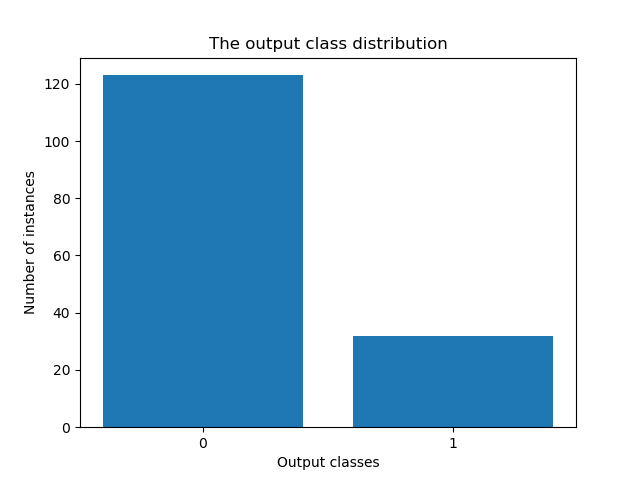
\includegraphics[width=0.6\textwidth]{Hep_Class.png}
				\caption{The class distribution of the output of the hepatitis dataset.}
				\label{fig:HepClass}
			\end{figure}
			
			\item \textit{Numeric feature distributions} (Figure \ref{fig:HepDist}) \\
			These distributions show very clearly how the feature values are distributed and that normalisation and standardisation should be considered to remove the feature value imbalance.
			
			\begin{figure}[H]
				\centering
				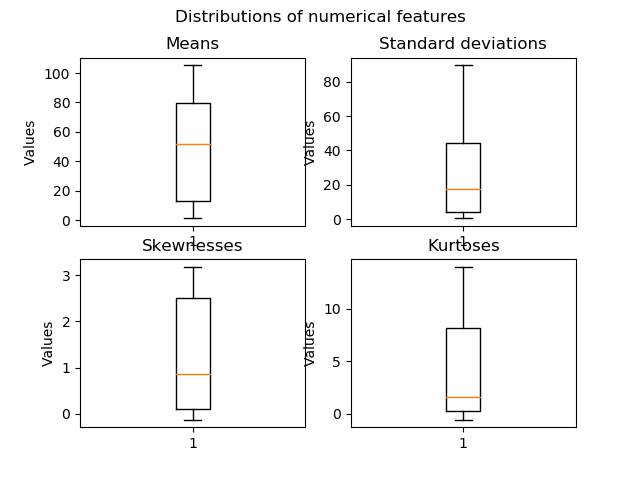
\includegraphics[width=0.8\textwidth]{Hep_Dist.png}
				\caption{The boxplots of the means, standard deviations, skewnesses and kurtoses from the features of the hepatitis dataset.}
				\label{fig:HepDist}
			\end{figure}
			
			\item \textit{Categorical and numeric cardinality} (Figures \ref{fig:HepCardCat} and \ref{fig:HepCardNum}) \\
			The distributions for the cardinality outliers mentioned at the start of this section are shown, but not very relevant in this case. No additional information can be found in this case.
			
			\begin{figure}[H]
				\centering
				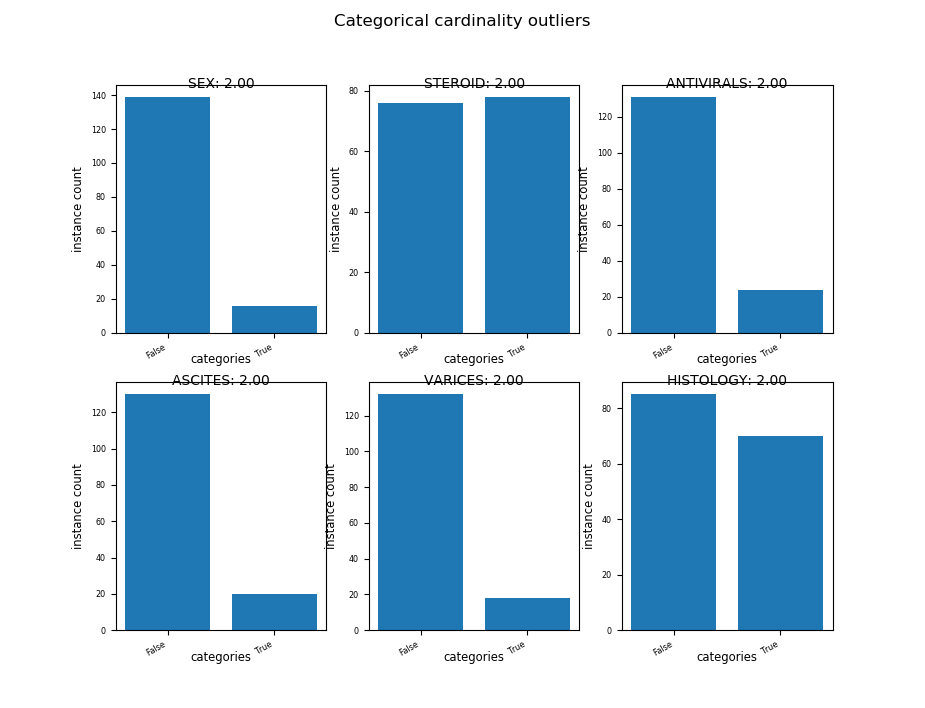
\includegraphics[width=0.8\textwidth]{Hep_Card_Cat.png}
				\caption{Histograms of the categorical features with either the highest or the lowest cardinality in the hepatitis dataset.}
				\label{fig:HepCardCat}
			\end{figure}
			
			\begin{figure}[H]
				\centering
				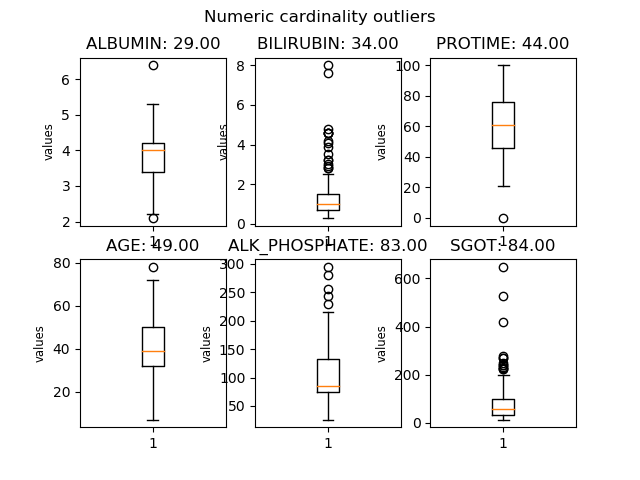
\includegraphics[width=0.8\textwidth]{Hep_Card_Num.png}
				\caption{Boxplots of the numeric features with either the highest or the lowest cardinality in the hepatitis dataset.}
				\label{fig:HepCardNum}
			\end{figure}
			
			\item \textit{Attribute entropy outliers} (Figures \ref{fig:HepAttEntCat} and \ref{fig:HepAttEntNum}) \\
			Especially the figure for categorical distributions show very well how features differ in entropy. The features \textit{SEX}, \textit{VARICES} and \textit{ASCITES} show a strong bias towards the value FALSE. The other three maximum outliers are far more balanced.
			
			\begin{figure}[H]
				\centering
				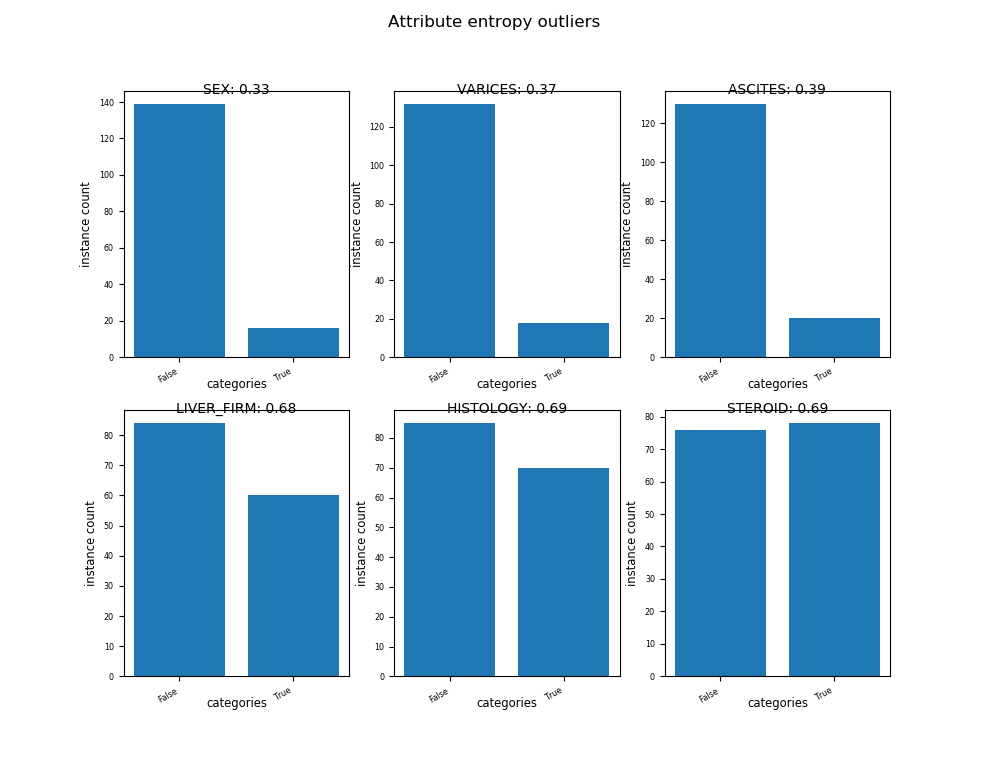
\includegraphics[width=0.8\textwidth]{Hep_AttEnt_Cat.png}
				\caption{Histograms of the categorical features with either the highest or the lowest attribute entropy in the hepatitis dataset.}
				\label{fig:HepAttEntCat}
			\end{figure}
			
			\begin{figure}[H]
				\centering
				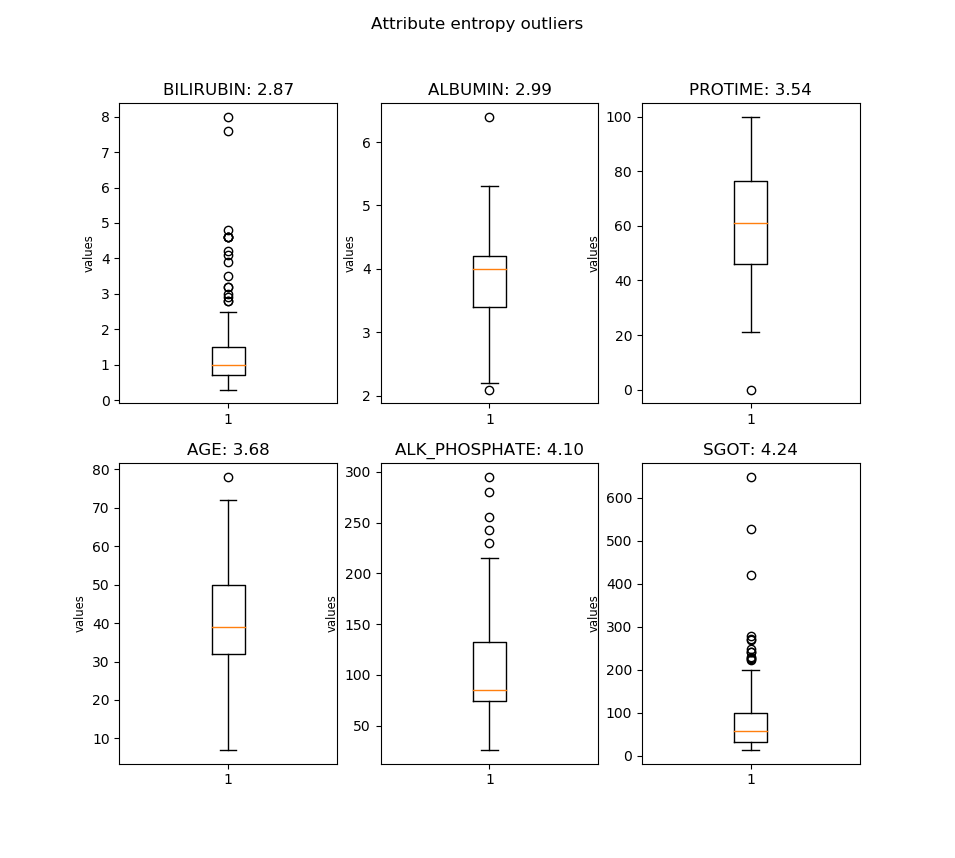
\includegraphics[width=0.8\textwidth]{Hep_AttEnt_Num.png}
				\caption{Boxplots of the numeric features with either the highest or the lowest attribute entropy in the hepatitis dataset.}
				\label{fig:HepAttEntNum}
			\end{figure}
			
		\end{enumerate}
		
	\end{itemize}
	
	% Final results
	Looking at the overall additional results, the following characteristics of \textit{metalearn} are improved with regard to exploration. More insight in correlation is given by using the correlation meta-features and several features are known to most likely be irrelevant or to the contrary very relevant. Also the understanding of the issues is better with the outliers, histograms and the boxplots.
	
	% Micro-organisms
	\subsubsection{Micro-organisms Dataset}
	\label{DEsubsec:AdditionalResultMO}
	
	% Introduction
	The additions are shown and discussed per different theme. First the correlation is discussed, followed by the minimum cardinality. Thirdly the outliers are discussed and lastly the plots.
	
	\begin{itemize}
		\item \textit{Correlation:} \\
		
		Due to the imposed restriction of combinatorial explosion, correlation will not be checked for more than 1000 features, and this dataset has 1300 features.
		
		\item \textit{Minimum cardinality} \\
		\underline{Minimum cardinality feature count:} 218 \\
		
		A total of 218 features have a cardinality of one and therefore do not contain any information.
		
		\item \textit{Outliers:} \\
		(Table \ref{tab:MOOutliers})
		
		All outliers are computed and the lowest and highest three outliers are shown (Table \ref{tab:MOOutliers}). Some results need further discussion:
		
		\begin{enumerate}
			\item The 20 possible class probabilities show no extreme outliers. Imbalance is still present, but there is no majority problem.
			\item The feature \textit{V1261} has the most potential information and has the second to most mutual information and therefore is a feature to keep an eye on.
			\item Again the features with one distinct value are found in the lowest outliers.
			\item The closeness in entropy and mutual information for the top three features shows that far more features are interesting to look at and that these features would be useful.
		\end{enumerate}
		
		\begin{table}[h]
			\caption{The outliers for the micro-organisms dataset}
			\label{tab:MOOutliers}
			\resizebox{\textwidth}{!}{
				\begin{tabular}{l|lll|lll}
					& \multicolumn{3}{l|}{\textbf{Lower bound}}                                                                                                                                                                                          & \multicolumn{3}{l}{\textbf{Upper bound}}                                                                                                                                                                                              \\ \cline{2-7} 
					\textbf{\begin{tabular}[c]{@{}l@{}}Outlier\\ Type\end{tabular}}                                                 & \textbf{\begin{tabular}[c]{@{}l@{}}First\\ Outlier\\ (name)\end{tabular}} & \textbf{\begin{tabular}[c]{@{}l@{}}Second\\ Outlier\\ (name)\end{tabular}} & \textbf{\begin{tabular}[c]{@{}l@{}}Third\\ Outlier\\ (name)\end{tabular}} & \textbf{\begin{tabular}[c]{@{}l@{}}Third\\ Outlier\\ (name)\end{tabular}}   & \textbf{\begin{tabular}[c]{@{}l@{}}Second\\ Outlier\\ (name)\end{tabular}} & \textbf{\begin{tabular}[c]{@{}l@{}}First\\ Outlier\\ (name)\end{tabular}}  \\ \hline
					\multicolumn{1}{|l|}{\textbf{\begin{tabular}[c]{@{}l@{}}Ratio of instances\\ with missing values\end{tabular}}} & \multicolumn{1}{l|}{--}                                                   & \multicolumn{1}{l|}{--}                                                    & --                                                                        & \multicolumn{1}{l|}{--}                                                     & \multicolumn{1}{l|}{--}                                                    & \multicolumn{1}{l|}{--}                                                    \\ \hline
					\multicolumn{1}{|l|}{\textbf{\begin{tabular}[c]{@{}l@{}}Ratio of features\\ with missing values\end{tabular}}}  & \multicolumn{1}{l|}{--}                                                   & \multicolumn{1}{l|}{--}                                                    & --                                                                        & \multicolumn{1}{l|}{--}                                                     & \multicolumn{1}{l|}{--}                                                    & \multicolumn{1}{l|}{--}                                                    \\ \hline
					\multicolumn{1}{|l|}{\textbf{Class probabilities}}                                                              & \multicolumn{1}{l|}{\begin{tabular}[c]{@{}l@{}}0.02\\ (7)\end{tabular}}   & \multicolumn{1}{l|}{\begin{tabular}[c]{@{}l@{}}0.02\\ (6)\end{tabular}}    & \begin{tabular}[c]{@{}l@{}}0.03\\ (9)\end{tabular}                        & \multicolumn{1}{l|}{\begin{tabular}[c]{@{}l@{}}0.09\\ (19)\end{tabular}}    & \multicolumn{1}{l|}{\begin{tabular}[c]{@{}l@{}}0.09\\ (3)\end{tabular}}    & \multicolumn{1}{l|}{\begin{tabular}[c]{@{}l@{}}0.11\\ (11)\end{tabular}}   \\ \hline
					\multicolumn{1}{|l|}{\textbf{\begin{tabular}[c]{@{}l@{}}Categorical\\ cardinality\end{tabular}}}                & \multicolumn{1}{l|}{--}                                                   & \multicolumn{1}{l|}{--}                                                    & --                                                                        & \multicolumn{1}{l|}{--}                                                     & \multicolumn{1}{l|}{--}                                                    & \multicolumn{1}{l|}{--}                                                    \\ \hline
					\multicolumn{1}{|l|}{\textbf{\begin{tabular}[c]{@{}l@{}}Numeric\\ cardinality\end{tabular}}}                    & \multicolumn{1}{l|}{\begin{tabular}[c]{@{}l@{}}1\\ (V1)\end{tabular}}     & \multicolumn{1}{l|}{\begin{tabular}[c]{@{}l@{}}1\\ (V447)\end{tabular}}    & \begin{tabular}[c]{@{}l@{}}1\\ (V1090)\end{tabular}                       & \multicolumn{1}{l|}{\begin{tabular}[c]{@{}l@{}}259\\ (V1261)\end{tabular}}   & \multicolumn{1}{l|}{\begin{tabular}[c]{@{}l@{}}294\\ (V719)\end{tabular}}  & \multicolumn{1}{l|}{\begin{tabular}[c]{@{}l@{}}296\\ (V838)\end{tabular}}  \\ \hline
					\multicolumn{1}{|l|}{\textbf{\begin{tabular}[c]{@{}l@{}}Correlation\\ combinations\end{tabular}}}               & \multicolumn{1}{l|}{--}                                                   & \multicolumn{1}{l|}{--}                                                    & --                                                                        & \multicolumn{1}{l|}{--}                                                     & \multicolumn{1}{l|}{--}                                                    & \multicolumn{1}{l|}{--}                                                    \\ \hline
					\multicolumn{1}{|l|}{\textbf{\begin{tabular}[c]{@{}l@{}}Categorical\\ attribute entropy\end{tabular}}}          & \multicolumn{1}{l|}{--}                                                   & \multicolumn{1}{l|}{--}                                                    & --                                                                        & \multicolumn{1}{l|}{--}                                                     & \multicolumn{1}{l|}{--}                                                    & \multicolumn{1}{l|}{--}                                                    \\ \hline
					\multicolumn{1}{|l|}{\textbf{\begin{tabular}[c]{@{}l@{}}Numeric\\ attribute entropy\end{tabular}}}              & \multicolumn{1}{l|}{\begin{tabular}[c]{@{}l@{}}0.0\\ (V1)\end{tabular}}   & \multicolumn{1}{l|}{\begin{tabular}[c]{@{}l@{}}0.0\\ (V1099)\end{tabular}}  & \begin{tabular}[c]{@{}l@{}}0.0\\ (V212)\end{tabular}                      & \multicolumn{1}{l|}{\begin{tabular}[c]{@{}l@{}}0.60\\ (V1163)\end{tabular}} & \multicolumn{1}{l|}{\begin{tabular}[c]{@{}l@{}}0.62\\ (V1002)\end{tabular}} & \multicolumn{1}{l|}{\begin{tabular}[c]{@{}l@{}}0.83\\ (V1261)\end{tabular}} \\ \hline
					\multicolumn{1}{|l|}{\textbf{\begin{tabular}[c]{@{}l@{}}Categorical\\ joint entropy\end{tabular}}}              & \multicolumn{1}{l|}{--}                                                   & \multicolumn{1}{l|}{--}                                                    & --                                                                        & \multicolumn{1}{l|}{--}                                                     & \multicolumn{1}{l|}{--}                                                    & \multicolumn{1}{l|}{--}                                                    \\ \hline
					\multicolumn{1}{|l|}{\textbf{\begin{tabular}[c]{@{}l@{}}Numeric\\ joint entropy\end{tabular}}}                  & \multicolumn{1}{l|}{\begin{tabular}[c]{@{}l@{}}2.91\\ (V1)\end{tabular}}  & \multicolumn{1}{l|}{\begin{tabular}[c]{@{}l@{}}2.91\\ (V1071)\end{tabular}} & \begin{tabular}[c]{@{}l@{}}2.91\\ (V782)\end{tabular}                     & \multicolumn{1}{l|}{\begin{tabular}[c]{@{}l@{}}3.34\\ (V1163)\end{tabular}} & \multicolumn{1}{l|}{\begin{tabular}[c]{@{}l@{}}3.35\\ (V1002)\end{tabular}} & \multicolumn{1}{l|}{\begin{tabular}[c]{@{}l@{}}3.49\\ (V1261)\end{tabular}} \\ \hline
					\multicolumn{1}{|l|}{\textbf{\begin{tabular}[c]{@{}l@{}}Categorical\\ mutual information\end{tabular}}}         & \multicolumn{1}{l|}{--}                                                   & \multicolumn{1}{l|}{--}                                                    & --                                                                        & \multicolumn{1}{l|}{--}                                                     & \multicolumn{1}{l|}{--}                                                    & \multicolumn{1}{l|}{--}                                                    \\ \hline
					\multicolumn{1}{|l|}{\textbf{\begin{tabular}[c]{@{}l@{}}Numeric\\ mutual information\end{tabular}}}             & \multicolumn{1}{l|}{\begin{tabular}[c]{@{}l@{}}0.00\\ (V1)\end{tabular}}  & \multicolumn{1}{l|}{\begin{tabular}[c]{@{}l@{}}0.00\\ (V251)\end{tabular}} & \begin{tabular}[c]{@{}l@{}}0.00\\ (V248)\end{tabular}                     & \multicolumn{1}{l|}{\begin{tabular}[c]{@{}l@{}}0.25\\ (V787)\end{tabular}} & \multicolumn{1}{l|}{\begin{tabular}[c]{@{}l@{}}0.25\\ (V1261)\end{tabular}} & \multicolumn{1}{l|}{\begin{tabular}[c]{@{}l@{}}0.27\\ (V1008)\end{tabular}} \\ \hline
				\end{tabular}
			}
		\end{table}
		
		\item \textit{Plots} \\
		
		The values for the plots are computed and visualized. Whereas these plots do not show any additional information, they do further clarify earlier mentioned problems (Subsection \ref{DEsubsec:ExistingResultMO})
		
		\underline{Class count histogram:} Figure \ref{fig:MOClass} \\
		
		The class count histogram shows that most of the classes are around 25 to 30 instances. There are however seven classes that have significant more or less instances.
		
		\begin{figure}[]
			\centering
			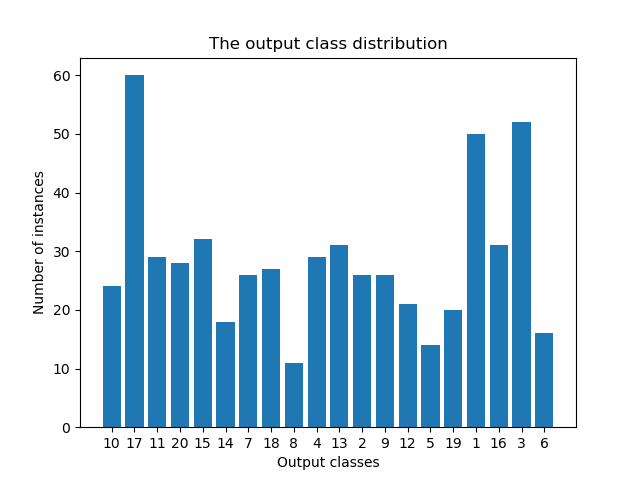
\includegraphics[width=0.8\textwidth]{MO_Class.png}
			\caption{The class distribution of the output of the micro-organisms dataset.}
			\label{fig:MOClass}
		\end{figure}
		
		\underline{Distribution boxplots:} Figure \ref{fig:MODist} \\
		
		These boxplots show very well the difference in values for every feature. The creation of a boxplot of the means and standard deviation and the high number of outliers, show that normalisation or standardisation seems a good preprocessing action.
		
		\begin{figure}[]
			\centering
			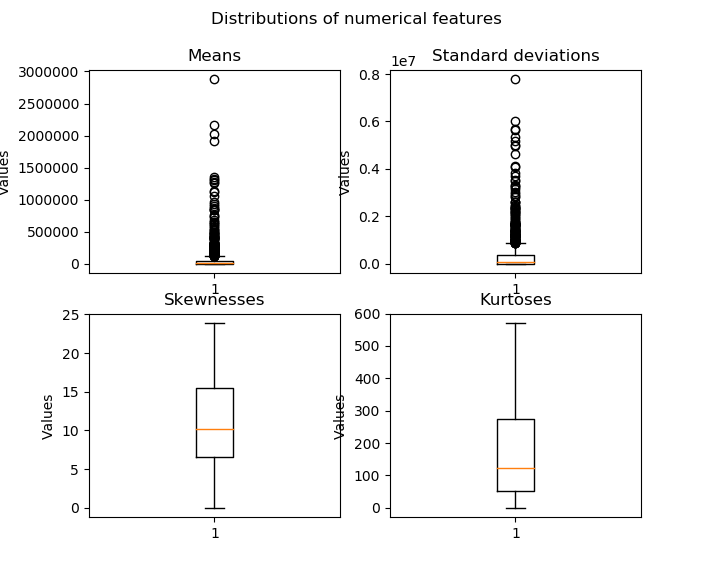
\includegraphics[width=0.8\textwidth]{MO_Dist.png}
			\caption{The boxplots of the means, standard deviations, skewnesses and kurtoses from the features of the micro-organisms dataset.}
			\label{fig:MODist}
		\end{figure}
		
		\underline{Numeric cardinality outlier boxplots:} Figure \ref{fig:MOCardNum} \\
		
		The numeric cardinality boxplots show very well how the feature values are distributed. Due to this dataset originating from mass spectrometry, most values are 0. All values that are not 0 can become significantly high, with outliers having a factor $10^7$. Again the outliers with the lowest cardinality have just one value, 0.
		
		\begin{figure}[]
			\centering
			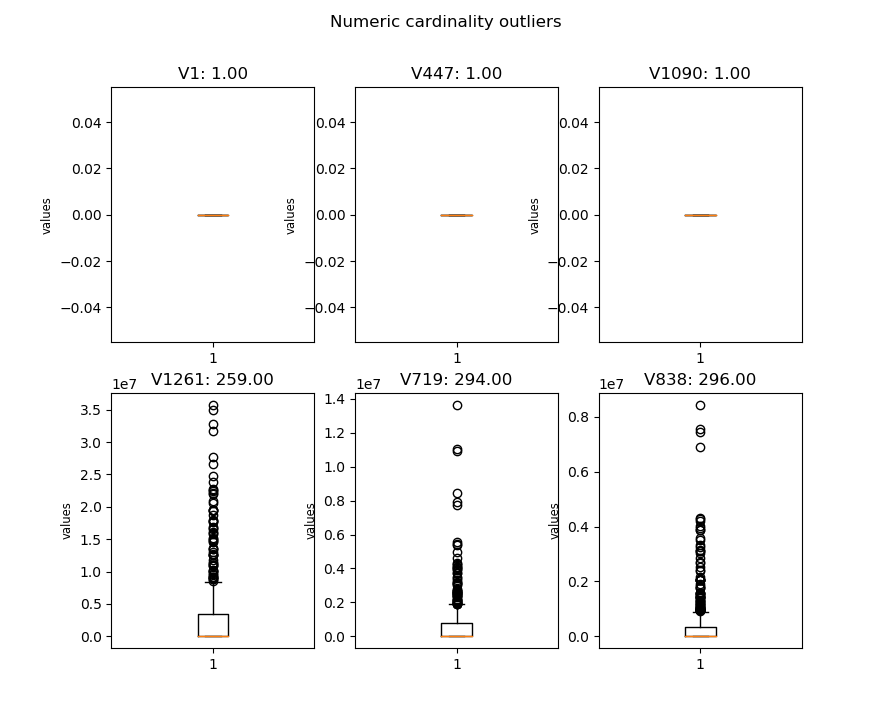
\includegraphics[width=0.8\textwidth]{MO_Card_Num.png}
			\caption{Boxplots of the numeric features with either the highest or the lowest cardinality in the Micro-organisms dataset.}
			\label{fig:MOCardNum}
		\end{figure}
		
		\underline{Numeric attribute entropy boxplots:} Figure \ref{fig:MOAttEntNum} \\
		
		The attribute entropy outliers cannot directly be seen in the box plot. This plot does not seem very useful in this case.
		
		\begin{figure}[]
			\centering
			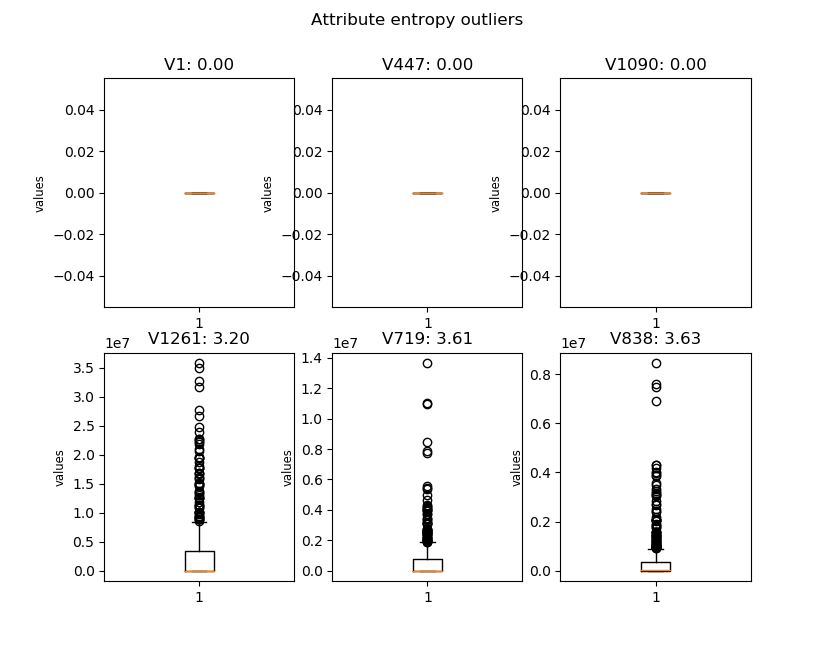
\includegraphics[width=0.8\textwidth]{MO_AttEnt_Num.png}
			\caption{Boxplots of the numeric features with either the highest or the lowest attribute entropy in the Micro organisms dataset.}
			\label{fig:MOAttEntNum}
		\end{figure}
		
	\end{itemize}	
	
	% Final results
	First, finding out that 218 features in the dataset that contain no information is very useful in initial understanding of the dataset. The outliers mainly show that most likely many more features are useful in finding a good result. The histograms and boxplots are more useful as they give a better view in the class distribution. They also visualize the distributions of both the means, standard deviations and also the feature distributions, giving more understanding and insights.
	
	\section{Discussion}
	\label{DEsec:Discussion}
	
	% Differences in dataset
	There are numerous ways biomedical datasets are gathered and therefore numerous issues that can be found in the dataset. The six discussed issues are well known and therefore a good representation, however there are more issues. For example the issue of having too few instances and trying to generate more is not discussed nor the possibility of anomalies being present in the data. These two issues may be addressed in future research.
	
	% 
	
	\section{Conclusions}
	\label{DEsec:Conclusions}
	
	% Introducion
	In this chapter the package \textit{metalearn} was analysed and additional content for the package was made to further improve its capabilities. The analysis was done with regard to the possibility to locate dataset issues with the meta-features present.
	
	% Hypotheses
	The first hypothesis H1 is confirmed, in that all issues except for multicollinearity were found in the two datasets with the current meta-features. Multicollinearity needed more addressing besides these meta-features. The information from the meta-features was tough to understand, though. The sheer number of the meta-features made it hard to find the issues, and the lack of examples and visualization made it hard to understand how these issues are manifested in the dataset. Therefore H2 is also confirmed.
	
	% Additions
	The problem posed in the confirmed H2 and the lack of multicollinearity testing in H1 was partly removed by the addition of new meta-features, outliers and histograms and boxplots. These made a better understanding, showed several features that needed more attention and also showed better if multicollinearity could be a problem for the dataset. Therefore the additions are useful in dataset exploration.
	
	% Framework
	\textit{Metalearn} with the added changes was able to sufficiently locate dataset issues. On top of that its ease of use and simplicity in understanding result in \textit{metalearn} to be a useful addition to the framework.
	
	\chapter{Framework Overview}
	\label{chap:FrameworkImplementation}
	
	\section{Introduction}
	\label{FIsec:Introduction}
	
	% Introduction
	With the results of the feature selection, missing value handling and data exploration research, a guideline framework is made to incorporate these results. The framework is based on four phases: a dataset type challenge explanation, a dataset exploration, a preprocessing step and automated analysis. Every phase has its own framework questions for which information or methods are available. A layout of the framework is also given to point out all its options (Figure \ref{fig:FrameworkLayout}).
	
	\begin{figure}
		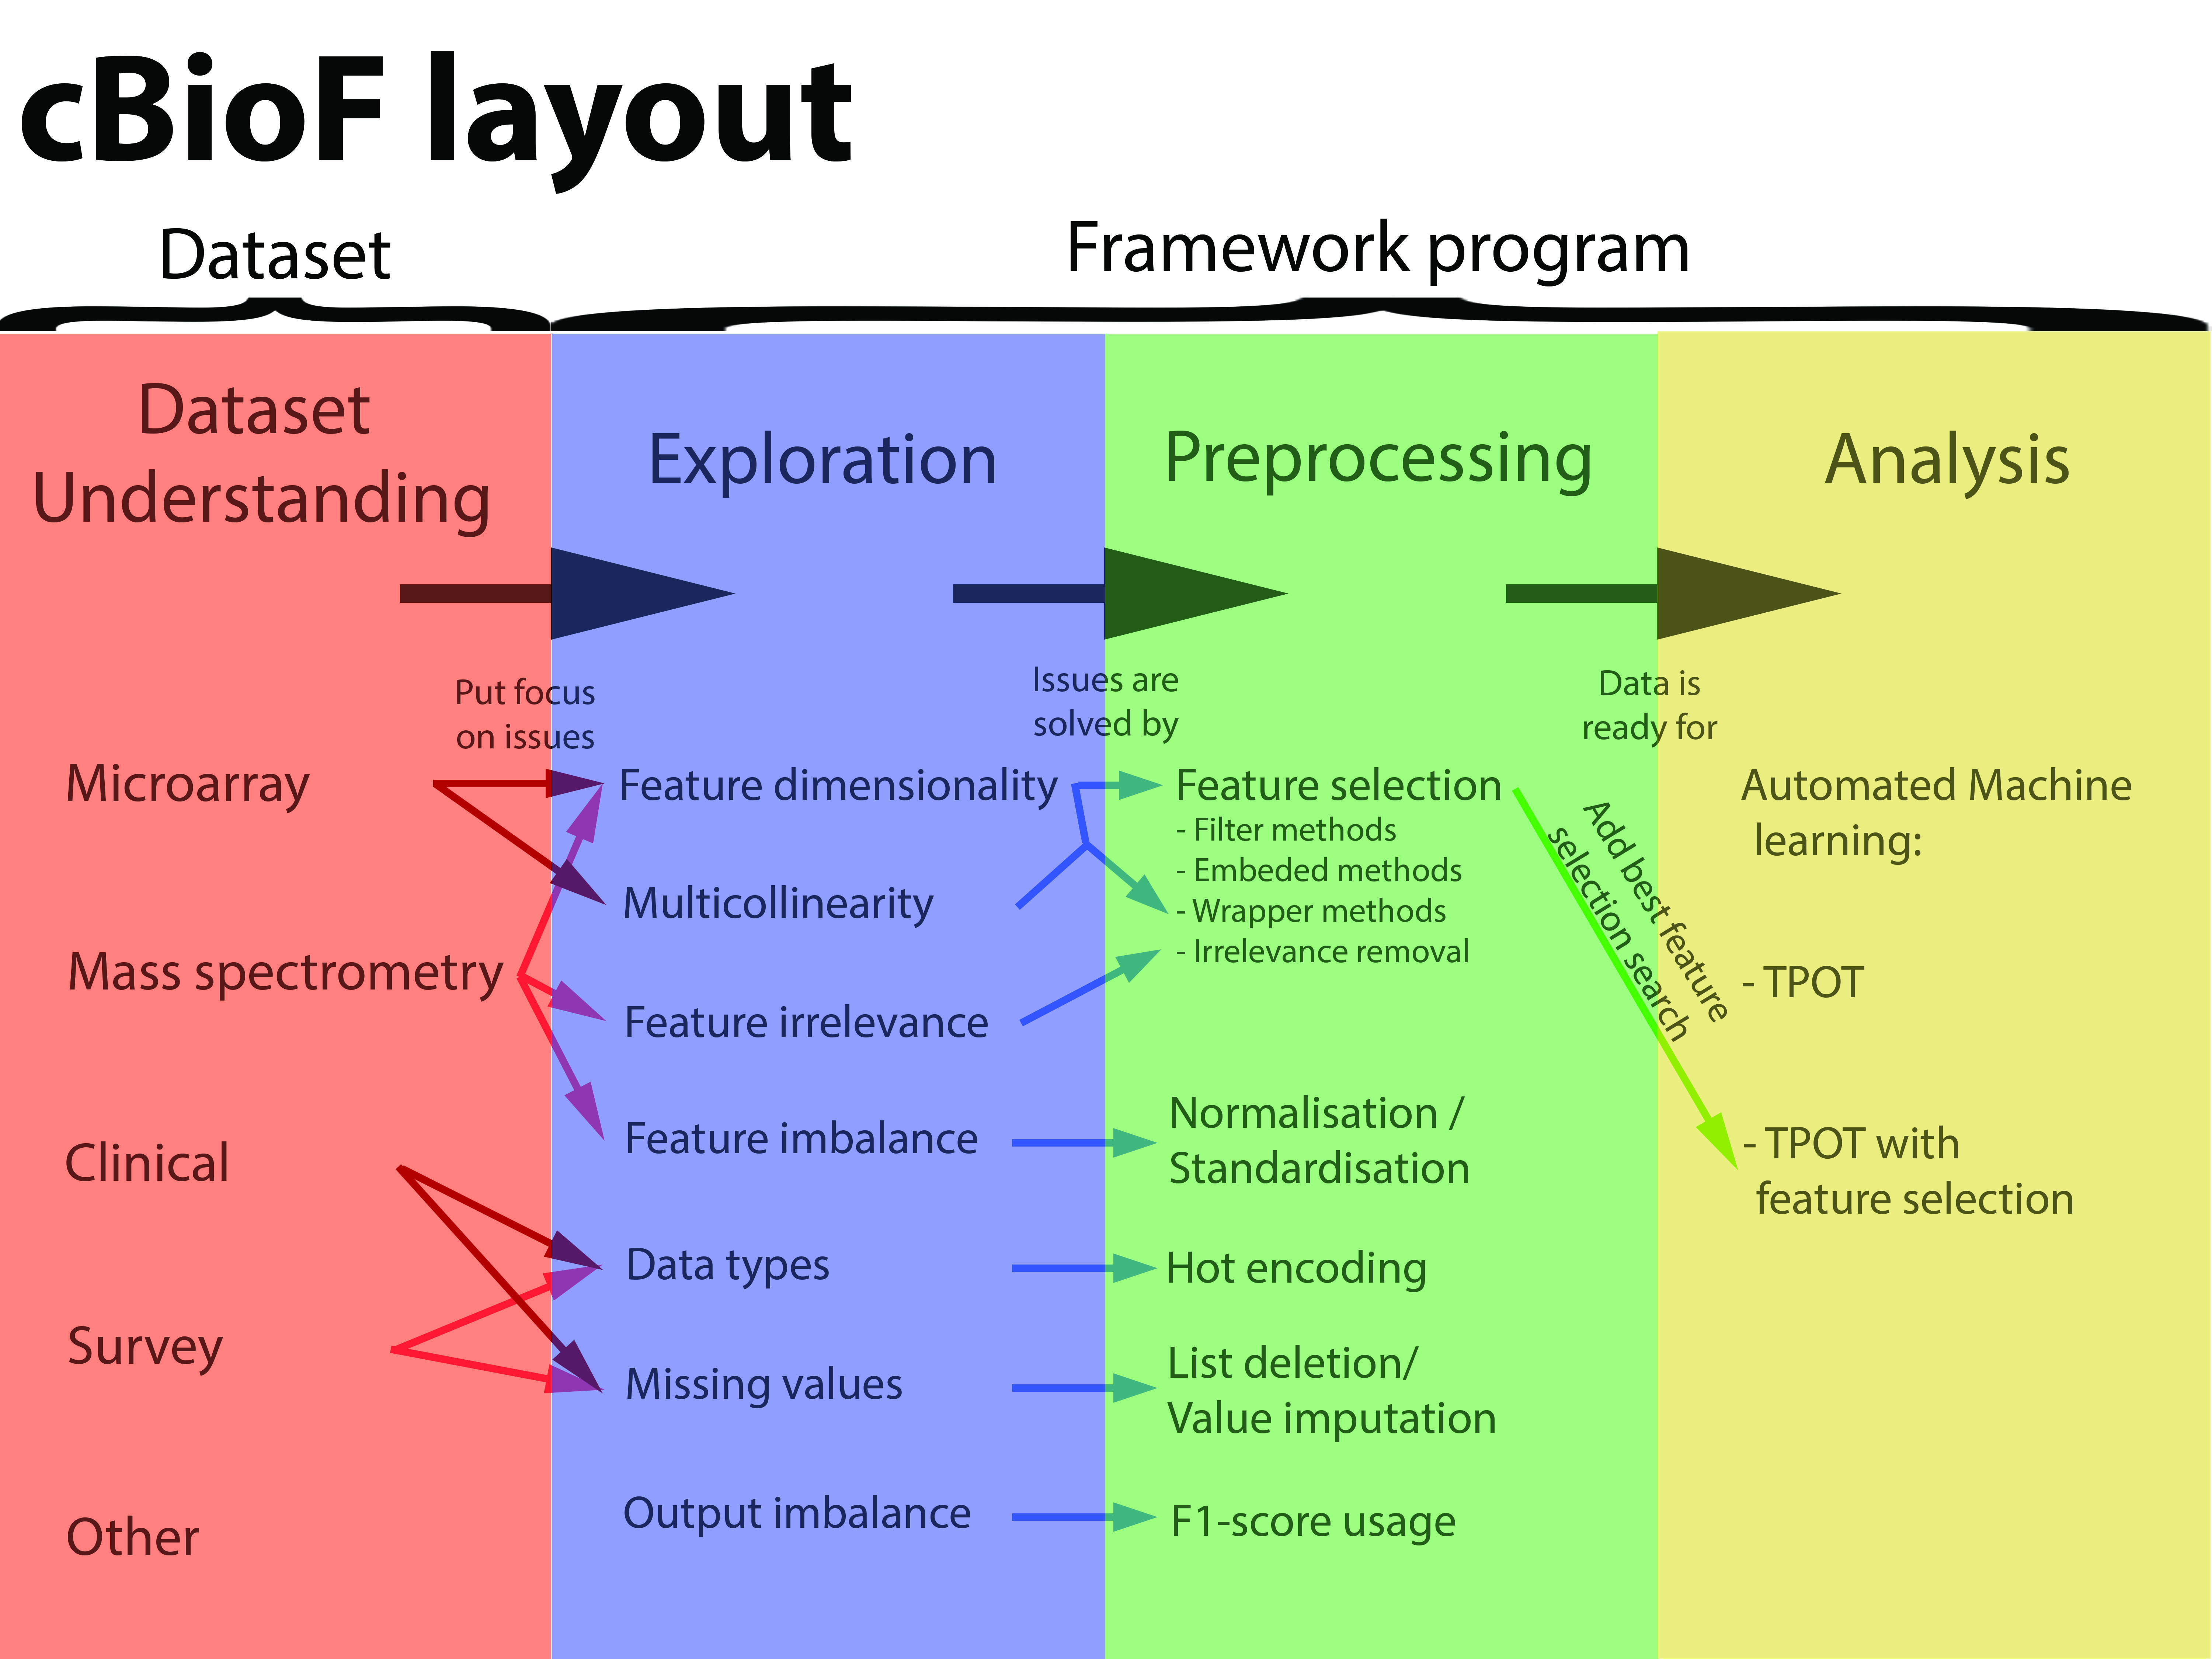
\includegraphics[width=\linewidth]{FrameworkLayout.jpg}
		\caption{A graphical layout of the framework showing all aspects presented.}\label{fig:FrameworkLayout}
	\end{figure}
	
	% Ground rules framework
	This framework is mainly for guiding a data analyst into the first phases of his analysis. The dataset is understood and preprocessed quicker and some initial machine learning analyses are given. The steps exploration, preprocessing and analysis in the framework are also automated with the simple preprocessing and machine learning algorithms for ease of use. Further analysis in both preprocessing and machine learning however is advised, as usually datasets need a more specific analysis to find good results. 
	
	% Framework set-up
	This framework is set up for datasets for which the data is given in a matrix. In this matrix every column corresponds to a feature and every row corresponds to a data sample. Data should be adjusted such that it satisfies the required input format. Finally it is worth emphasizing that the framework is developed with the assumption that classification problems are solved. Some techniques are also applicable for regression however and those parts in the framework can still be used for those.
	
	\section{Dataset type}
	\label{FIsec:DatasetType}
	
	Before analysing any of the data, some information can be retrieved from the dataset origin. Different types of datasets usually encompass potential issues being present (Section \ref{PLsec:Datasets}). An initial framework question is therefore implied to address these potential issues: \\
	\\
	% Framework Question
	\emph{FQ1: What type of dataset is used?} \\

	Several different datasets are used and all potential issues should be investigated. Four dataset types however are previously investigated and for each of these types a specific focus on a selection of issues is given. Both the dataset types and the possible extra focus on dataset issues are shown (Figure \ref{fig:FrameworkLayout}).
	
	\begin{enumerate}
		\item[A] \textit{Micro-array dataset} \\
		Micro-array data usually consists of a high number of genes being investigated. Most of those genes are not of use in this work, therefore feature selection is a useful way of removing the irrelevant genes. Due to this high number of genes possible computation time issues can occur in some algorithms. These computation time issues would also be reduced when only a few features are selected. Furthermore, genes are most likely very related to each other as well, showing high values for multicollinearity. 
		\item[B] \textit{Mass spectrometry dataset} \\
		Mass spectrometry usually consists of a high number proteins being investigated, resulting in a high number of features. Feature selection therefore is a useful way of removing irrelevant proteins. Mass spectrometry often does not detect any presence of a protein, when they are tested for. Therefore initially several proteins can be removed for not containing any information. This should be explored at the start. At last, peaks in the mass spectrometry data are very high in variance and the dataset would benefit from normalisation to remove this difference.
		\item[C] \textit{Clinical dataset} \\
		There are very different clinical datasets, therefore potential issues are harder to pin down. Usually clinical datasets are not created by the data analyst however, therefore possibly creating mismatches on that part. The data types within the dataset can be different, having categorical, ordinal and numerical data. Hot encoding categorical data helps future analysis in this case. Also missing values are sometimes present, so missing value handling might be useful. 
		\item[D] \textit{Survey dataset} \\
		Survey dataset usually do not lack a number of instances, but do have other problems. Missing values are often present because of people not properly filling out all answers and therefore missing value handling is something to keep in mind. Survey datasets mostly contain categorical and ordinal data, but can also have numerical data. Hot encoding the categorical and ordinal data will make analyses with numeric methods possible. 
	\end{enumerate}
	
	\section{Dataset Exploration}
	\label{FIsec:ExplorationResults}
	
	% Introduction	
	Exploration of the data is the next step in the framework to perform. This exploration will show whether several specific issues are present (Chapter \ref{chap:DatasetExploration}). This results in the following framework question: \\
	\\
	% Framework Question
	\emph{FQ2: What possible dataset issues can be present?} \\
	
	This is done by computing meta-features of the dataset using \textit{metalearn}. These meta-features lead to seven different dataset issues. These issues are added to the framework layout (Figure \ref{fig:FrameworkLayout}). Links to preprocessing methods to solve them are added as well.
	
	\begin{enumerate}
		\item[A] \textit{Feature dimensionality} \\
		The dimensionality is checked as well as the mutual information present between data and output. If the dimensionality is high (more features than labels), features with a very low mutual information with the output can undesirably overshadow more useful features.
		
		\item[B] \textit{Multicollinearity} \\
		Multicollinearity is present if the features contain common information. This is found by doing principal component analysis and correlation checking. If the first three principal components contain a significant amount of explained variance or if features have a high correlation, multicollinearity most likely is present.
		
		\item[C] \textit{Feature irrelevance} \\
		To find out if there are features that do not contain any information, the cardinality for all features is checked. If features are present with a cardinality of one, irrelevant features are present. These features are not useful in any way and should better be removed.
		
		\item[D] \textit{Feature imbalance} \\
		If the mean and standard deviation are significantly different in numeric features, bias can be present when analysing the dataset. How to cope with this is different for a normal distribution compared with not normal distributions. Therefore skewness and kurtosis can be used to find out if the features follow a normal distribution or not. 
		
		\item[E] \textit{Data types} \\
		The type of features can be different within the dataset. Since all analyses done in this study use numeric data, categorical data are not useful to have in the dataset.
		
		\item[F] \textit{Missing values} \\
		Missing values can be present in the dataset. Since the presentation of missing values can be very different, it also might be hard to find these missing values. %Alternatively a list of possible missing value indicators are given in the exploration. The presence of missing values is checked, as well as the fractions of instances and features having them. 
		
		\item[G] \textit{Output imbalance} \\
		By looking at the output classes, possible imbalance can be found. This imbalance shows possible bias when creating prediction results regarding false positive and negatives.
		
	\end{enumerate}

	The exploration and preprocessing of these seven issues give the user a lot of insight in the data, as well as the possibility to quickly overcome them. Therefore the user can quickly start trying out analysis techniques to get the desired results.
	
	\section{Preprocessing}
	\label{FIsec:Preprocessing}
	
	% Introduction	
	After exploration of the dataset, the issues that are found must be removed. The following framework question is about dataset preprocessing: \\
	\\
	% Framework Question
	\emph{FQ3: What techniques can be used to overcome dataset issues?} \\
	
	Five possible solutions are given to overcome these issues. In the framework, these solutions can also be done automatically and in those cases generic solutions are used. The solutions are also shown, together with their influence in analysis, if present (Figure \ref{fig:FrameworkLayout}).
	
	\begin{enumerate}
		\item[A] \textit{Feature selection} \\
		Feature selection is a logical step to filter out unuseful features and preserve useful ones when a high dimensionality is present. For preprocessing this is fixed by doing a filter method  or an embedded method. If multicollinearity is also present, a wrapper method can better be used, as it also takes into account multicollinearity (Chapter \ref{chap:FeatureSelection}). At last, if irrelevant features are present, they can be simply removed by removing all features with a cardinality of 1. In automated preprocessing a simple filter method with ANOVA is used for feature selection without multicollinearity, otherwise a wrapper method with forward selection is used after ordering the data from most to least useful.
		
		\item[B] \textit{Normalisation/Standardisation} \\
		To remove the feature imbalance, the data can be normalised or standardised. It is standardised when not following a normal distribution and normalised when it is following a normal distribution. When it is a normal distribution, the mean and standard deviation are investigated separately to find out if the data needs to be normalised for both.
		
		\item[C] \textit{Hot encoding} \\
		To change categorical features into numeric ones, all categorical data are hot encoded into numeric data.		
		
		\item[D] \textit{List deletion/Value imputation} \\
		To handle missing values, several list deletion algorithms and value imputation algorithms are available. If only a relatively low number of instances or features have missing values, CCA or ACA is the best methods to use. Otherwise a value imputation algorithm is preferred (Chapter \ref{chap:MissingValueHandling}). CCA or ACA are used when the number of missing values is at most 10\% for either instances or features respectively, when preprocessing automatically. Otherwise a mean imputation method is used. In that mean imputation however, features are removed if they have more than 15\% missing values, due to not properly being represented.
		
		\item[E] \textit{Robust score usage}
		When this imbalance is present, the user is advised to use an alternative score system than the standard accuracy, for example the F1-score.		
		 
	\end{enumerate}
	
	\section{Automated Analysis}
	\label{FIsec:Analysis Recommendations}
	
	% Introduction
	After exploring and preprocessing the dataset, the next step would be to find a good analysis technique to find the desired results. Machine learning is a good approach for that, as it tries to predict the behaviour of a phenomenon by using the available data. Which technique should be used to predict this behaviour however is different for every dataset and result and therefore multiple analyses might be needed to find the correct one. Therefore the last framework question is implied: \\
	\\
	% Framework Question
	\emph{FQ4: What technique can be best used to analyse the dataset?} \\
	
	% Automated machine learning
	One way to find the correct technique is using automated machine learning (Chapter \ref{chap:FeatureSelection}, Figure \ref{fig:FrameworkLayout}). Automated machine learning tries to automatically find the best machine learning technique to predict the behaviour. On top of that, it also combines techniques and also tests out additional preprocessing methods for possible better results. The package \textit{TPOT} is a tool that implements automated machine learning and can be used. 
	
	% Feature selection option
	There is no best feature selection algorithm. Because of that a \textit{TPOT} extension is made to select the best feature selection algorithm for the dataset. This extension multiplies the output with a penalty on the number of features. Also two additional features are added for further enhancing the search for the best feature selection algorithm. First the possibility of a feature selection favoured start is given, so the automated machine learning starts with a bias in feature selection. Secondly a new set of feature selection algorithms is given that focuses on preserving at most 200 features (Chapter \ref{chap:FeatureSelection}). This way the user can select which combination of feature selection rules are needed for his dataset.	
	
	\chapter{Conclusions}
	\label{chap:Conclusions}
	
	% Introduction
	This work discusses three research topics, each of them having their own conclusions. In this chapter these conclusions are combined and recommendations for future research are given. These conclusions are used in the corresponding parts of the framework (Chapter \ref{chap:FrameworkImplementation}), which is the main contribution of this thesis. In what follows the main contributions and conclusions are summarized for every research line.
	
	\begin{itemize}
		\item \textit{Feature Selection} (Chapter \ref{chap:FeatureSelection})  \\
		Experiments were conducted involving feature selection methods. This resulted in four conclusions.
	\begin{itemize}
		\item No significant difference in quality was found between using mutual information or T-test/ANOVA when using filter methods. Mutual information took longer to compute, but T-test/ANOVA assumed normal distributions, so both should be considered. Also for filter methods, no more than 200 features were needed to explain the mass spectrometry and microarray datasets. Additional features added little to the prediction quality and were therefore not needed.
		\item Wrapper methods unexpectedly outperformed filter methods and embedded methods on everything but computation time. This difference in performance was due to wrapper methods removing multicollinearity. Filter and embedded methods performed very similar and seem to be the best choice when a lower computation time is desired and no dependencies are expected to be present. 
		\item There are differences between wrapper methods. Backwards and stochastic methods took much more computation time than forward methods and therefore are not worth using. This difference in computation time was also found comparing floating methods and forward and PTA methods. The difference in computation time was much lower, though, and floating methods did result in a higher output quality. The $\alpha$ threshold value, indicating the sensitivity of adding and removing features to the optimal feature set, was inversely correlated with the quality. A higher $\alpha$ indicated a lower quality, but preserved fewer features.
		\item The Tree-based Pipeline Optimisation Tool (\textit{TPOT}) showed a significantly better performance when using the improvements and for both very high number of features (50.000) and lower number of features (1.000-10.000) a better performance was found.
	\end{itemize}
			
	% Missing values
	\item \textit{Missing Value Handling} (Chapter \ref{chap:MissingValueHandling}) \\
	% H1
	Experiments involving missing value handling methods were done as well. These experiments resulted in three conclusions.
	\begin{itemize}
		\item The feature distributions were not preserved enough when using list deletion methods. Imputation methods preserved feature distributions better, especially k-nearest neighbour imputation.
		\item % Removal if more missing values
		A conclusion was made on how to handle features with high percentages of missing values, indicating two thresholds for ratio of missing values. Features with at least 40\% missing values should be removed, because of the bias created. Features with at least 15\% missing values are highly recommended to be removed.
		\item Conclusions were made based on the quality of the result. List deletion methods performed worse than imputation methods, as expected. Interestingly mean imputation outperformed more complex imputations, having similar quality but much lower computation time. 
	\end{itemize}
	
	\item \textit{Dataset exploration} (Chapter \ref{chap:DatasetExploration})\\
	% Exploration
	Two conclusions were made based on the analyses on dataset exploration.
	\begin{itemize}
		\item Almost all discussed dataset issues could be found using the meta-features provided by the package \textit{metalearn}. Multicollinearity was the only issue that was not clearly investigated.
		\item Additional meta-features as well as the addition of outliers and plots gave the user a better insight in his dataset, as well as a better investigation in multicollinearity. This extra insight made the user have a better focus on what the possibilities are present for his dataset.
	\end{itemize}

	\end{itemize}
	
	\section{Future Work}
	\label{CCsec:Discussions}
	
	% Feature selection
	
	% 200 features, why?
	In feature selection the first experiment shows that when using filter methods only 200 features must be preserved. This absolute number is not intuitive and much lower than expected. More research can be done on these preserved 200 features and why no other features are needed to predict the output. Cluster analyses for example may show insights in this phenomenon.
	
	% Combinations
	Also in feature selection only separate feature selection methods were tested. Whereas the filter methods needed very little computation time, the feature subset size and quality of the wrapper methods are much more interesting for further research. A combination of a filter and a wrapper method might create a better result. If first the majority of the features is filtered out by a filter method and then a wrapper method computes the best combination of feature, the result could be relatively quicker than the wrapper method while still maintaining a high enough quality. This combination is worth investigating in future research.
	
	% missing values
	
	% Datasets
	For missing value handling the datasets played a huge part in evaluation quality. Intuitively, precise imputation with the advanced missing value handling algorithms should outperform the less precise imputation of the simple algorithms. If the more precise imputation is done for an irrelevant feature value, though, the extra information will not produce a better output. Future research can be done on datasets with missing values that are known to be very important for the result to find out if this assumption holds for these datasets.
	
	% Framework
	
	% Multicollinearity
	Dataset issues mentioned in this thesis are addressed in the framework and preprocessing methods or recommendations are given. A preprocessing method for multicollinearity however is only given in combination with feature selection, no preprocessing method only focusing on multicollinearity is present. Future research is needed to find a technique to cope with multicollinearity when feature selection is not needed.
	
	% Other dataset issues
	There are more possible dataset issues than the aforementioned ones. Examples are anomalies in the data or having too few samples to analyse the data. These issues are not explored and the framework cannot properly remove these issues by preprocessing. Therefore it would benefit from future research such that these unexplored issues and possibilities to overcome them can be added. 
	
	\bibliography{../References/Citings} 
	\bibliographystyle{ieeetr}
	
	\appendix
	
	\chapter{Abbreviations}
	\label{PLsec:Abbreviations}
	
	Abbreviations used in the report as well as a location to find more information of these concepts if possible.
	
	\begin{itemize}
		\item \textit{ACA} - Available Case Analysis (Subsection \ref{MVsubsec:MissingValueHandling})
		\item \textit{ANOVA} - ANalysis of VAriances (Appendix \ref{app:BiomedicalDataAnalysis})
		\item \textit{CCA} - Complete Case Analysis (Subsection \ref{MVsubsec:MissingValueHandling})
		\item \textit{kNN} - k-Nearest Neighbours (TO DO STILL)
		\item \textit{LD} - List Deletion (Subsection \ref{MVsubsec:MissingValueHandling})
		\item \textit{MAR} - Missing At Random (Subsection \ref{MVsubsec:MissingValueHandling})
		\item \textit{MCAR} - Missing Completely At Random (Subsection \ref{MVsubsec:MissingValueHandling})
		\item \textit{MI} - Mutual Information (Section \ref{PLsec:Concepts})
		\item \textit{MICE} - Multiple Imputation Chained Equations (Subsection \ref{MVsubsec:MissingValueHandling})
		\item \textit{ML} - Machine Learning 
		\item \textit{MuI} - Multiple Imputation (Subsection \ref{MVsubsec:MissingValueHandling})
		\item \textit{NMAR} - Not Missing At Random (Subsection \ref{MVsubsec:MissingValueHandling})
		\item \textit{PTA} - Pick-l-Take-Away-r method (Subsection \ref{FSsubsec:FeatureSelectionMethods})
		\item \textit{RF} - Random Forests (Subsection \ref{FSsubsec:FeatureSelectionMethods})
		\item \textit{SI} - Single Imputation (Subsection \ref{MVsubsec:MissingValueHandling})
		\item \textit{SVM} - Support Vector Machines (Subsection \ref{FSsubsec:FeatureSelectionMethods})
		\item \textit{TPOT} - Tree-based Pipeline Optimisation Tool (Subsection \ref{FSsubsec:TPOT})
		\item \textit{WCA} - Weighted Case Analysis (Subsection \ref{MVsubsec:MissingValueHandling})
	\end{itemize}
	
	
	\chapter{Biomedical Data Analysis}
	\label{app:BiomedicalDataAnalysis}
	
	\section{Introduction}
	
	% Quick explanation for graduation project
	At the Computational Biology department (cBio) of Biomedical Engineering (BME), many requests are made to analyse gathered data. This data usually stems from research in hospitals, but also data from other research groups and publicly known data. With the vast number of data sets that are available, a framework on data analysis would be valuable. This framework would improve efficiency of this data analysis, as it would help choosing the best analysis approaches. 
	
	% Explanation for this document
	Before this framework is made however, first extensive research must be done on the already available analysis techniques. Many different approaches are used by researchers. These should be searched for and compared with each other, first using literature and second by actual use. This document focuses mainly on the literature part and explores the different techniques by analysing the articles.
	
	% Document lay-out
	At first the focus will mainly be on statistical methods. Different 
	techniques will be explained as well as the programs that can be used for 
	these statistical techniques. The second topic will be about machine 
	learning, and more specifically deep learning. 
	
	\clearpage
	
	\section{Statistical Analysis}
	
	% Quick summary of statistical analysis
	Statistical analysis consists of statements derived from large data sets that are often visualized in tables, graphs and charts. These statements are made on the basis of hypotheses and the analyses that either back up or reject those. The available data sets need to have a reasonably sized population so the statistical hypotheses can be tested.  \cite{woolson2011statistical} 
	
	% When to use statistical analysis? -- Find a reference for this
	The statistical approach is mainly used for drawing conclusions on the 
	data. When focusing on summarizing the data, inductive conclusions can be 
	made which then can be used in the biomedical world. Techniques that are 
	specifically useful for biomedical data are all combined in the term 
	biostatistics.  \cite{woolson2011statistical} 
	
	% The way data should look like
	To be able to use statistical analysis, the data should be quantitative. The data should be a population of data points and usually the size influences the accuracy of the outcome. Since most biomedical data stems from experiments on patients, the data usually is quantitative and can be analysed by statistical techniques.  \cite{sapsford2006data}
	
	% Chapter layout
	In this statistical analysis chapter, first some concepts are discussed. 
	Since for every data set the to be used computations are different, only 
	the basic ones are used to keep the report from irrelevant explanations. 
	Afterwards, five different programs or frameworks are discussed for their 
	approach to statistical analyses. Afterwards these five are compared by 
	literature and by personal testing.
	
	\clearpage
	
	\subsection{Statistical Research Topics}
	
	% Introduction statistical research
	Statistical research on its own has many applications. A selection of those 
	that are relevant for Biomedical data are discussed in here. Important in 
	statistical analysis is the presence of hypotheses. When doing this 
	analysis, the researcher has an expectation of the outcome. An example of 
	this would be having a data set of people of age and number of 
	grandchildren. The hypothesis could be: \textit{$H_0$: There is a 
		correlation between people's age and the number of grandchildren.} Then at 
	the end this or an alternate hypothesis $H_1$ can be either validated or 
	rejected. \cite{heiberger2004statistical}
	
	\subsubsection{Descriptive Statistics}
	
	% Introduction of descriptive statistics
	Descriptive statistics is a collection of methods for data analysis based around its variables. Data set variables are either numeric (categorical or grouped), ordinal (Ranked relatively) or continuous (Ranked with equal intervals). Descriptive statistics takes these variables and computes details of their distribution (Table \ref{tab:DescrStatEx}).  \cite{FISHER200993} These then summarize the data for the scientist analysing it. The newly created summary can be used for further statistical research, for example by comparing different populations or variables.  \cite{woolson2011statistical}
	
	\begin{table}[h!]
		\centering
		\caption{Descriptive Statistics examples \cite{FISHER200993}}
		\label{tab:DescrStatEx}
		\begin{tabular}{|l|l|l|l}
			\cline{1-3}
			\textbf{\begin{tabular}[c]{@{}l@{}}Variable \\ distribution\end{tabular}} & \textbf{\begin{tabular}[c]{@{}l@{}}Analysis terms \\ Center oriented\end{tabular}} & \textbf{\begin{tabular}[c]{@{}l@{}}Analysis terms\\ Spreading oriented\end{tabular}}                            &  \\ \cline{1-3}
			Numeric                                                                                           & Mode                                                                                                       & Frequency distribution                                                                                                                  &  \\ \cline{1-3}
			Ordinal                                                                                           & \begin{tabular}[c]{@{}l@{}}Median \\ Mode\end{tabular}                                                     & \begin{tabular}[c]{@{}l@{}}Frequency distribution\\ Percentiles\\ Minimum/Maximum\\ Range\end{tabular}                                  &  \\ \cline{1-3}
			Continuous                                                                                        & \begin{tabular}[c]{@{}l@{}}Mean\\ Median\\ Mode\end{tabular}                                               & \begin{tabular}[c]{@{}l@{}}Frequency distribution\\ Percentiles\\ Quartiles\\ Minimum/Maximum\\ Range\\ Standard Deviation\end{tabular} &  \\ \cline{1-3}
		\end{tabular}
	\end{table}
	
	% Visualization of descriptive statistics
	Aside from the aforementioned summary of the variables, descriptive statistics also consists of methods to properly visualize those. For numeric and ordinal data, histograms (Figure \ref{fig:HistEx}) and bar charts are often use to show in a easily understandable way how they are distributed. For continuous data box plots (Figure \ref{fig:BoxEx}) can be used as well to show specific details of the distribution.  \cite{dupont2009statistical}
	
	\begin{figure}[h!]
		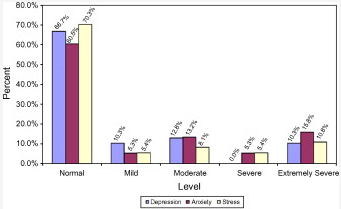
\includegraphics{HistogramExample.PNG}
		\caption{An example of a histogram of ordinal data. The depression, anxiety and stress scale of women with an acute coronary syndrome is shown. the data shows that over sixty percent rates themselves as normal.  \cite{FISHER200993}}
		\label{fig:HistEx}
	\end{figure}
	
	\begin{figure}[h!]
		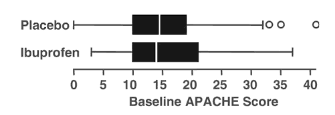
\includegraphics{BoxplotExample.PNG}
		\caption{An example of a box plot of continuous data. The distribution of the APACHE score (Acute Physiology And Chronic Health Evaluation) was given for users of ibuprofen and placebo. The box plot doe snot only show the minimum, maximum and mean, but also quartiles and possible outliers.  \cite{dupont2009statistical}}
		\label{fig:BoxEx}
	\end{figure}
	
	\subsubsection{Probability Concepts}
	
	% Introduction
	When using biomedical data, it usually contains some phenomena that seem random and affect data values. Modelling and analysis of those data phenomena is hard, due to his unpredictability. A probabilistic approach can be used to tackle this.  \cite{shiavi2010introduction}
	
	% Probability meaning
	Values that seems to have a random part can be measured multiple times. 
	When looking at multiple measurements an average can be found within their 
	distribution in the sample space. The probability of a value to be within a 
	certain interval is always a number between 0 and 1. The probability of a 
	value to be in the sample space is 1, as it the complete interval. 
	 \cite{shiavi2010introduction}
	
	% Probability Distributions
	Another aspect of probability is about the several distributions. These 
	show the total probability for a value to be on a certain interval. There 
	are two different kinds of probability distributions: discrete and 
	continuous. The difference between these two is the spacing between the 
	possible values. Values from continuous distributions can take every value, 
	whereas values from discrete distributions are limited and the possible 
	values have spacings between them. \cite{heiberger2004statistical}
	
	% Binomial distribution
	Binomial distribution is the most common example of a discrete distribution 
	(Figure \ref{fig:BinomDistEx}). This distribution can be seen as a number 
	of $n$ independent trials that have a success rate of $p$, with $p$ being a 
	number on the interval $(0,1)$. This distribution has a mean of $\mu = np$ 
	and standard deviation of $\sigma = \sqrt{np(1-p)}$. 
	 \cite{heiberger2004statistical}
	
	\begin{figure}[h!]
		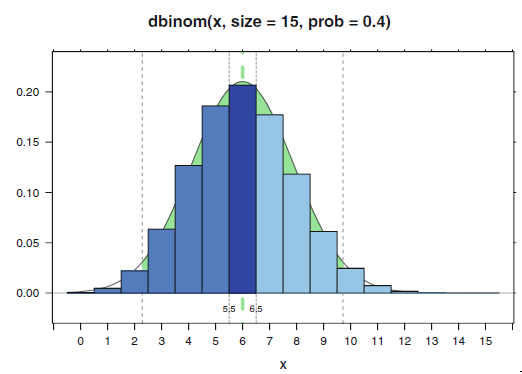
\includegraphics[scale=0.5]{BinomDistExample.PNG}
		\caption{An example of a binomial distribution, a discrete probability 
			distribution. In this example there were $n =  15$ trials with a 
			success rate of $p = 0.4$.  \cite{heiberger2004statistical}}
		\label{fig:BinomDistEx}
	\end{figure}
	
	% Normal distribution
	The most common continuous probability distribution is called a normal 
	distribution (Figure \ref{fig:NormDistEx}). This distribution is bell 
	shaped and symmetric around the mean $\mu$, with a standard deviation 
	$\sigma$. The standard normal distribution $Z$ has a $\mu = 0$ and $\sigma 
	= 1$ and can be made with a modification on a regular normal distribution 
	$X$: $Z = \frac{X-\mu}{\sigma}$.  \cite{heiberger2004statistical}
	
	\begin{figure}[h!]
		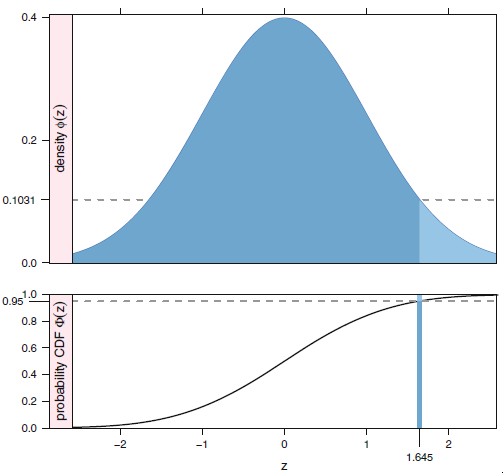
\includegraphics[scale=0.5]{NormDistExample.PNG}
		\caption{An example of a normal distribution, a continuous probability 
			distribution. This example is the standard normal distribution with 
			mean $\mu =  0$ and standard deviation $\sigma = 1$. 
			 \cite{heiberger2004statistical}}
		\label{fig:NormDistEx}
	\end{figure}
	
	% Student's T distribution
	The third distribution that will be discussed is the student's 
	t-distribution, another continuous distribution (Figure 
	\ref{fig:StudTDistEx}). This one is very similar 
	to the normal distribution discussed earlier. The student's t distribution 
	has a sample size of $n$ and a sample standard deviation of $s$. The 
	standard distribution can be found with the formula $Z = \frac{X-\mu}{s / 
		\sqrt{n}}$ The larger the sample size $n$, the closer $s$ will get to 
	$\sigma$ of a normal distribution, so an infinite sample size $n$ is a 
	normal distribution. \cite{heiberger2004statistical}
	
	\begin{figure}[h!]
		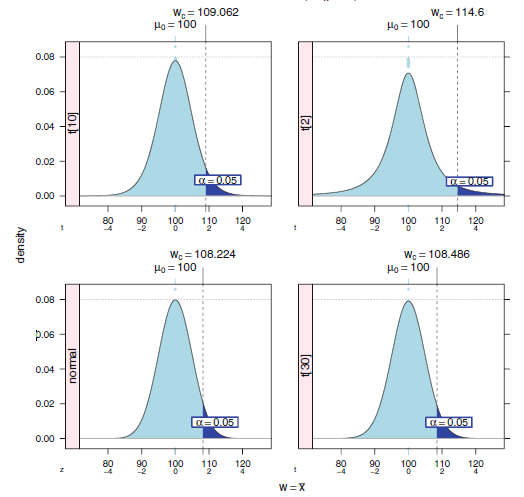
\includegraphics[scale=0.5]{StudTDistExample.PNG}
		\caption{An example of a 3 student's t distributions and a normal 
			distribution. With an sample size $n$ becoming higher, the standard 
			deviation $s$ comes closer to normal distribution standard deviation 
			$\sigma$.  \cite{heiberger2004statistical}}
		\label{fig:StudTDistEx}
	\end{figure}
	
	% Famous tests that find out the goodness of fit
	Several tests are used to find out if a data set can be fits a certain 
	distribution. The "Goodness of fit" is then tested. The Chi-Square and 
	Kolmogorov Smirnov are such tests. There may be more powerful and 
	specialized ones though, for example the Shapiro Wilk for normality 
	testing.  \cite{heiberger2004statistical}
	
	\subsubsection{Interval testing}
	
	%Introduction
	On the previously discussed probability distributions specific intervals 
	can be computed. A confidence interval can show the interval where a 
	certain value should be in. This can be done for an unknown mean of a 
	distribution or an unknown population proportion in a t distribution. These 
	intervals are made similar to this one, the confidence interval of the 
	mean, with 
	mean $\hat{y}$, confidence number $z$, percentage cut-off $\alpha$, 
	standard deviation $\sigma$ and 
	population sample $n$ (Equation \ref{eq:CI}). \cite{heiberger2004statistical}
	
	\begin{equation}
	\label{eq:CI}
	(\hat{y} - z_{\frac{\alpha}{2}}\frac{\sigma}{\sqrt{n}}, \hat{y} + 
	z_{\frac{\alpha}{2}}\frac{\sigma}{\sqrt{n}})
	\end{equation}	
	
	\subsubsection{Group comparisons}
	
	% Introduction
	The previously discussed confidence intervals can be used to find out 
	whether two data sets are similar in terms of mean and variance. If the 
	confidence intervals of the means of both data sets then the two data sets 
	could be describing the same distribution. Its independence can then be 
	proven by comparing their confidence intervals. 
	 \cite{heiberger2004statistical}
	
	% Explanation comparison mean
	The independence has two different parts. Two data sets can be independent 
	comparing their means and they can be independent comparing their 
	variances. The more important one of the two is when means are compared, as 
	then they can be substantially different. To test whether two data sets are 
	independent on their mean, a series of tests can be done ( 
	\ref{tab:IndepTest}). For these tests it makes a difference whether the 
	unknown variance is common, different or the data is 
	paired. \cite{heiberger2004statistical}
	
	\begin{table}[h!]
		\centering
		\caption{Formulas to compute whether two samples are independent by means. 
			The parameters $s_{\Delta\bar{y}}$ and $t_{calc}$ can be three different 
			values (Table \ref{tab:sdyandtcalc}) \cite{heiberger2004statistical}. The values for the mean $\mu$, }
		\label{tab:IndepTest}
		\begin{tabular}{llllll}
			\hline
			&  & 
			\multicolumn{2}{l}{\textbf{Tests}} & 
			\textbf{Confidence Interval} & \textbf{}               \\ \cline{3-6} 
			\textbf{H0}              & \textbf{H1}              & \textbf{Rejection 
				region}   & $p$-value                      & 
			\textbf{Lower}               & \textbf{Upper}          \\ \hline
			$\mu_1 \leq \mu_2$                  & $\mu_1 > \mu_2$       & 
			$t_{calc} 
			> t_\alpha$       & $P(t > t_{calc})$      & 
			$((\bar{y}_1 
			- \bar{y}_2) - t_\alpha s_{\Delta \bar{y}}$,       & 
			$\infty)$                     \\
			$\mu_1 \geq \mu_2$                  & $\mu_1 < \mu_2$          & 
			$t_{calc} 
			< -t_\alpha$          & $P(t < t_{calc})$         & 
			$(-\infty$,                        & $(\bar{y}_1 - \bar{y}_2) + 
			t_\alpha 
			s_{\Delta \bar{y}})$ \\
			$\mu_1 = \mu_2$                  & $\mu_1 \neq \mu_2$                  
			& 
			$|t_{calc}| > t_{\frac{\alpha}{2}}$     & $P(t >
			|t_{calc}|)$  & $((\bar{y}_1 - \bar{y}_2) - 
			t_{\frac{\alpha}{2}} 
			s_{\Delta\bar{y}}$ 
			,     & $(\bar{y}_1 - \bar{y}_2) + t_{\frac{\alpha}{2}} 
			s_{\Delta 
				\bar{y}})$  
			\\ 
			\hline
		\end{tabular}
	\end{table}
	
	\begin{table}[h!]
		\centering
		\caption{The values of $s_{\Delta\bar{y}}$ and $t_{calc}$ for data sets 
			with common unknown variance, uncommon unknown variance and paired 
			data.  \cite{heiberger2004statistical}}
		\label{tab:sdyandtcalc}
		\begin{tabular}{lll}
			\hline
			\textbf{Data set}  & \textbf{$s_{\Delta\bar{y}}$}     & 
			\textbf{$t_{calc}$}                                                
			\\ \hline
			Common variance    & $s_{\Delta\bar{y}} = s_p \sqrt{\frac{1}{n_1} + 
				\frac{1}{n_2}}$ & 
			$t_{calc} = \frac{\bar{y}_1-\bar{y}_2}{s_p \sqrt{\frac{1}{n_1} + 
					\frac{1}{n_2}}}         $                                      \\
			Different variance & $s_{\Delta\bar{y}} = s_{\bar{y}_1 - 
				\bar{y}_2}$    & 
			$s_{(\bar{y}_1-\bar{y}_2)} =\sqrt{\frac{s^2_1}{n_1} + 
				\frac{s^2_2}{n_2}}$, and $t_{calc} = \frac{\bar{y}_1 - 
				\bar{y}_2}{s_{(\bar{y}_1-\bar{y}_2)}}$ \\
			Paired data        & $s_{\Delta\bar{y}} = \bar{s}_d$           & 
			$s_{\bar{d}} = s_d / \sqrt{n}$, and $t_{calc} 	
			=\frac{\bar{d}}{s_{\bar{d}}}$                                       
			
			
			\\
			\hline
		\end{tabular}
	\end{table}
	
	% Explanation comparison variance
	To find out whether variances of two data sets could be common, a new value 
	$F$ is introduced with the formula $F = \frac{s_1^2}{s_2^2}$. Since this $F 
	= 1$ is the most ideal situation (both variances being equal), an equation 
	can be made in which the boundaries can be specified (Equation 
	\ref{eq:FVarInt}). In this equation $F_{low} = F_{1-\frac{\alpha}{2},n_1-1, 
		n_2-1}$ and $F_{high} =  F_{1-\frac{\alpha}{2},n_2-1, n_1-1}$, the upper 
	percentage points with the $n_1 - 1$ and $n_2 - 1$ or $n_2 -1$ and $n_1 - 
	1$ degrees of freedom respectively. 
	 \cite{heiberger2004statistical}
	
	\begin{equation}
	\label{eq:FVarInt}
	(\frac{s_1^2}{s_2^2}\frac{1}{F_{low}}, \frac{s_1^2}{s_2^2}F_{high})
	\end{equation}
	
	% Tests for data
	If data is paired (Table \ref{tab:IndepTest}), to test if their means are 
	paired is usually done with a t-test. A similar version, the two sample 
	t-test, is the way to go when the distribution is known of the data set. A 
	specific way to tests multiple groups at the same time is the one-way 
	analysis of variance (ANOVA). This t-test is preferred over other test due 
	to his power compared to the other tests.  \cite{heiberger2004statistical}
	
	% Tests for non-parametric (paired) data
	Data can also not follow any specific distribution. In those cases 
	Non-parametric statistical procedures will be used. An example would be the 
	Sign test, when a certain median is taken and found out if there are enough 
	data points above and under that median. This Sign test can also be used 
	with paired populations and find out whether there is a significant number 
	of data points from one of the sets lower than the data points from the 
	other set. An upgraded version of this Sign test is called Wilcoxon 
	Signed-Ranks Test, which also takes the magnitude of the data into 
	account. \cite{heiberger2004statistical}
	
	% Tests for non-parametric unpaired data
	If the data is not paired, the Mann-Whitney Test may be a good choice. This	
	test is related to the two sample t-test, however uses medians instead of 
	means. The more than two sample testing version of the Mann-Whitney Test is 
	the Kruskal-Wallis test. This test should be used if some of the 
	populations do not seem to be uniformly distributed enough for an ANOVA 
	test. \cite{heiberger2004statistical}
	
	\clearpage
	
	\subsection{Statistical Programs}
	
	\subsubsection{SAS}
	
	% SAS explanation
	Statistical Analysis System (\textit{SAS}) is a system used for statistical 
	analysis. It can be used to perform a big variety of those with ease. 
	Scientist can learn \textit{SAS} quickly to perform small statistical computations 
	for quick results. Within \textit{SAS} a variety of algorithms are available for 
	analysis. This simplicity of calling those algorithms makes \textit{SAS} very time 
	efficient.  \cite{o2013step}
	
	\subsubsection{SPSS}
	
	% SPSS explanation
	\textit{SPSS} is the statistical program with the most diverse users. \textit{SPSS} is very 
	user-friendly and easy to use when not familiar in either programming or 
	when the there is only need for basic statistical analysis. Due to these 
	advantages in educational research \textit{SPSS} is widely used, especially by the 
	social studies in need of these analysis techniques.  \cite{muijs2010doing}
	
	\subsubsection{R}
	
	% R explanation
	\textit{R} is one of the more well known statistical computing language for people who have experience in programming. It provides a language as well as statistical procedures to use for their analysis. Both \textit{SAS} and \textit{SPSS} created extensions for \textit{R}, so it can be used in theirs as well. This is less intuitive, due those two being very similar.  \cite{muenchen2011r}
	
	\subsubsection{Python}
	
	% Python explanation
	\textit{Python} is widely known for being an open source programming language with a 
	relatively low bar to learn it. It was not often used for scientific 
	analyses. Due to the maturity of several useful library as \textit{NumPy} and \textit{SciPy} 
	however, \textit{Python}'s market share is growing. Its open source element 
	increases the usability over time as well. At last, since \textit{Python} is also 
	used for other projects not involving statistics, scientists may already 
	know the language. 
	 \cite{mckinney2010data}
	
	\subsubsection{MATLAB}
	
	% Matlab explanation
	Matlab is not necessarily known for its statistical analysis, but more for 
	its good way of handling biomedical data. Biomedical scientists and 
	engineers are often familiar with \textit{MATLAB} and its clear way of writing 
	commands to analyse data. For statistical analysis extensions are 
	available, an example would be the computational statistics toolbox. Also 
	on the internet, many freely available user-created functions can be found, 
	which can be used to the scientist's advantage.
	 \cite{martinez2007computational}
	
	\subsubsection{Comparisons programs}
	
	% First example comparisons
	Many comparisons are made for scientists which statistical program is best 
	to use. A good scheme was made by Jeroen Kromme, a data scientist of 
	Cmotions that is involved with bringing data analysis to other scientists 
	(Figure \ref{fig:StatProgComp}). He compares the fairly accessible programs 
	\textit{SA}S and \textit{SPSS} with the more potential programs \textit{R} and 
	\textit{Python}. \cite{BlogKromme2017}
	
	\begin{figure}[h!]
		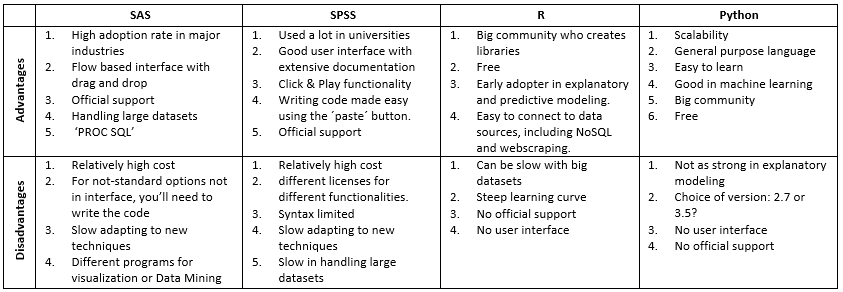
\includegraphics[width=\textwidth]{StatProgComp.PNG}
		\caption{Advantages and Disadvantages of the statistical programs \textit{SAS}, 
			\textit{SPSS}, \textit{R} and \textit{Python}. \cite{BlogKromme2017}}
		\label{fig:StatProgComp}
	\end{figure}
	
	% Second example comparisons
	Another article has been written by Kunal Jain that compares the 
	commercially used \textit{SAS} with the academic \textit{R} and the high potential \textit{Python}. 
	He rates the programs on different aspects with what he shows that \textit{Python} 
	has the best potential of the three (Figure 
	\ref{fig:StatProgGrades}). \cite{BlogJain2017}
	
	\begin{figure}[h!]
		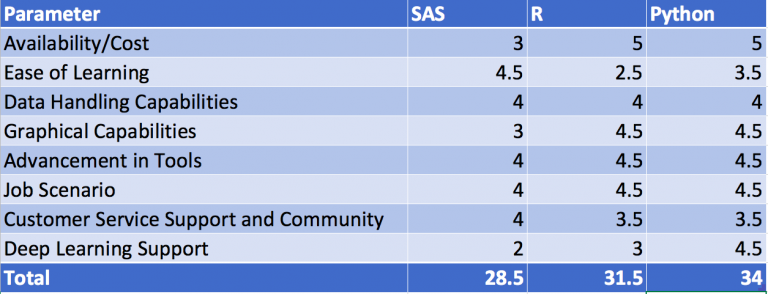
\includegraphics[width=\textwidth]{StatProgGrades.PNG}
		\caption{Grades for \textit{SAS}, \textit{R} and \textit{Python} on different aspects of using a 
			program for statistical analysis. \cite{BlogJain2017}}
		\label{fig:StatProgGrades}
	\end{figure}
	
	% Combinations of programs
	Combinations of the statistical programs is also possible. \textit{SAS} and \textit{SPSS} are 
	very similar to each other and switching between those is 
	not hard to do. Both of these use extensions that allows the user to work 
	with \textit{R} functions. This is useful as \textit{R} has more variety in their functions 
	compared with \textit{SAS} and \textit{SPSS}.
	 \cite{muenchen2011r}
	
	% Final comparisons
	These explained surveys and more  \cite{BlogWillems2014} 
	 \cite{BlogSupport2017} show that these programs all have a different 
	approach. \textit{SPSS} is used by the scientists and companies that don't need very 
	advanced techniques. \textit{SAS} extends the the usability of \textit{SPSS} by a little and 
	is provided by support, therefore companies that need a bit more advanced 
	statistical analyses prefer to use \textit{SAS}. \textit{R} is a widely known useful program 
	that is mainly used in the academic world by scientists that know a bit of 
	programming and need more in-depth analyses. \textit{Python} is not widely used, yet 
	but is on the rise due to its popularity for other programming sciences, as 
	well.
	
	\subsubsection{Personal comparisons}
	
	% Testing of statistical programs
	All of these statistical programs have been tested personally, too. This 
	was done in past projects for courses at the TU/e The 
	final comparisons of the articles match the outcome of those findings. 
	
	% Matlab, SPSS and SAS
	\textit{SPSS} and \textit{SAS} can do numerous things statistically, however it is still very 
	basic compared to R and \textit{Python}. Since biomedical engineers are known to 
	process their data in \textit{MATLAB} and \textit{Python}, it is not worth it to pre-process 
	data to use in \textit{SAS} and \textit{SPSS} when \textit{MATLAB} and \textit{Python} can do about the same 
	things. If the only need is fairly simple statistical computations, \textit{MATLAB} 
	will be sufficient for that. If the there is need for more complex 
	computations, \textit{SAS} and \textit{SPSS} most likely would not be able to do those easily 
	anyway 
	
	% R and \textit{Python}
	If more complex statistical analyses are needed, it would be smarter to 
	look at \textit{R} and \textit{Python} for use. They both work on a similar level and both 
	have an advantage over the other. If a scientist is not familiar with 
	complex statistical analyses or with either language, \textit{R} might be better for 
	him. \textit{R} is more widely used and therefore more material is available for 
	help. Scientists that do know \textit{Python} or are already working with it, are 
	better of doing the statistical analyses with \textit{Python}. There is no need 
	learning a new language when it would only take up more time.
	
	\clearpage
	
	\section{Deep Learning}
	
	% Introduction to Deep Learning
	As computers are becoming smarter and smarter, the idea of computers 
	learning how to tackle various problems is bigger than before. Also the 
	size of data sets is growing two, which makes current ways of extracting 
	information harder to use. The idea of 
	giving computers a way to learn from experience and teach them how to cope 
	with examples for treating real data the right way is called deep learning. 
	 \cite{Goodfellow-et-al-2016} Deep learning is structurally used more in the 
	biomedical environment to explain several concepts, especially considering 
	images and the usage of neural networks. \cite{greenspan2016guest}
	
	% Talking about Deep Learning topics
	The whole idea of a computer gaining experience from finding patterns in 
	the data is called machine learning. Deep learning is a sub section of 
	machine learning as deep learning tries to solve problems by combining 
	multiple small solutions. These small solutions are then connected in a 
	network, that is often called a artificial neural network (ANN), resembling 
	the neural network in a human brain. \cite{Goodfellow-et-al-2016}
	
	\clearpage
	
	\subsection{Basic Machine Learning}
	\label{subsec:MachineLearning}
	
	% Introduction
	As deep learning is a specific kind of machine learning, knowing the 
	important basics of machine learning is necessary. This is divided in three 
	different parts, the task, performance measurement and the experience 
	gained. \cite{Goodfellow-et-al-2016}
	
	\subsubsection{Tasks}
	
	% Task description
	The task of a machine learning program is to solve problems that can not be 
	solved by humans only. This way of solving requires a different mindset in 
	programming. The program must be made so it knows how to solve a problem 
	instead of manually telling the program how to solve it. Tackling a problem 
	in the case of machine learning usually is done by having it process 
	examples that are a collection of features. The example is a data point 
	which details are described by those features. What needs to be done with 
	those examples can be different. \cite{Goodfellow-et-al-2016}
	
	% Classification
	One task the program could do is specify a specific label from a number of 
	categories. The examples all should be divided between several groups and 
	machine learning tries to find the correct group for every example. This 
	can be done multiple ways. Examples are in a discrete way (every example 
	has one group) or in a probabilistic way (every example has a certain 
	chance to be part of some groups). \cite{Goodfellow-et-al-2016}
	
	% Regression
	Another task the program could do is predict a numerical value for the 
	examples. This is similar to classification only the answer is not limited 
	to a number of categories. Instead it can be any value on a numerical 
	interval.  \cite{Goodfellow-et-al-2016}
	
	% Other tasks
	Classification and regression are the most commonly used tasks within 
	machine learning. Other less used tasks could be to translate data to a 
	structured representation, to detect errors in the examples or remove noise 
	from the data. All off these tasks could be tackled using machine 
	learning. \cite{Goodfellow-et-al-2016}
	
	\subsubsection{Performance Measurement}
	
	%Introduction performance measurement
	When using machine learning, the performance of the algorithm is important. 
	The program should not only use the data to create output, but this output 
	must be correct as well. To measure this correctness, the accuracy is often 
	measured. This accuracy is the percentage of examples that give the correct 
	output. An error rate can be used as a performance measurement too, the 
	number of examples that give an incorrect 
	output. \cite{Goodfellow-et-al-2016}
	
	% Using a test set
	Data is used when training a machine learning algorithm. The algorithm is 
	made to be as effective as possible for this training data, therefore the 
	accuracy is supposed to be high for that data. This training data is 
	usually just a subset of all possible data though and therefore the actual 
	accuracy may be lower. To find this out, a separate test set can be made 
	alongside the training set. This test set is then only used to find this 
	accuracy. \cite{Goodfellow-et-al-2016}
	
	% Further performance discussion
	The performance measurements also require further thoughts than the 
	accuracy and test sets. It may very well be that some categories in 
	classifications are more important to be right (e.g. high risk patients) or 
	the penalty for big deviations in regression may be bigger than needed. 
	These things all need to be considered before measuring the accuracy. 
	 \cite{Goodfellow-et-al-2016}
	
	\subsubsection{Experience}
	
	% Introduction Experience
	There are superficially spoken two kinds of machine learning, unsupervised 
	or supervised. The difference between those is the experience they are 
	allowed to have during its training. This training is done with a specific 
	idea in mind that differs for these two 
	categories. \cite{Goodfellow-et-al-2016}
	
	% Unsupervised
	Unsupervised machine learning algorithms have the experience of a dataset 
	with many features. With these features it can create structures within 
	them. An example for this unsupervised learning would be clustering, to 
	group data in different clusters according to their 
	features. \cite{Goodfellow-et-al-2016}
	
	% Supervised
	When using supervised data an additional label or target is given in 
	addition to it regular features. With these, the algorithm knows what 
	outcome every data point should get and learns to achieve that output with 
	the available features.  \cite{Goodfellow-et-al-2016}
	
	\subsubsection{Challenges}
	
	% challenges machine learning
	Several challenges arise when using machine learning. Obvious challenges 
	are using the right algorithm, having a data set with enough data that is 
	also sufficiently detailed and and retrieving a good enough accuracy. 
	Eventually the goal is to have a high accuracy on the created test set. The 
	performance quality on the test set is called 
	generalization. \cite{Goodfellow-et-al-2016}
	
	
	% Errors
	There are three type of errors when working with an algorithm. At first 
	there is the training error, the error rate for training data. This 
	training error is always better than the test error, the error rate for the 
	test data. The difference between those is called the generalization error. 
	When an algorithm is made, the training error should be kept as low as 
	possible as well as the generalization error. \cite{Goodfellow-et-al-2016}
	
	
	% Challenges for these errors
	The challenge to have the training error as low as possible is to not under 
	fit, which means that the algorithm does not achieve a low enough training 
	error. The challenge for generalization error is to no over fit, which 
	means that the test error is not close enough to the training 
	error. \cite{Goodfellow-et-al-2016}
	
	\clearpage
	
	\subsection{Neural Networks}
	
	% Introduction neural networks
	The name neural networks stems from the connections between neurons in the 
	brain, a big research area in modern day biology. In the mathematical 
	world, artificial neural networks can be made for modelling data analysis. 
	These models that are created with the neural networks use a specific 
	equation (Equation \ref{eq:NeuralModels}). The output (computation) is a 
	combination of already stored information (storage), new information 
	(transmission) and process it with available methods in the model 
	(processing). \cite{rojas2013neural}
	
	\begin{equation}
	\label{eq:NeuralModels}
	\text{computation} = \text{storage} + \text{transmission} + 
	\text{processing}.
	\end{equation}
	
	% A neural network initial layout
	Zooming closer into neural networks, the idea of a single neuron can be 
	shown (Figure \ref{fig:NeurEx}). These neurons have three different 
	important parts. The first part are the input values $x_i$, which are first 
	modified a bit with weights $w_i$. The third part is the actual function 
	$f$ that creates output for the weighted input values. These neurons  then 
	put together create a network with eventually an output (Figure 
	\ref{fig:NeurNetEx}). \cite{rojas2013neural}
	
	\begin{figure}[h!]
		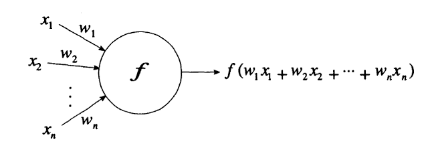
\includegraphics{NeuronExample.PNG}
		\caption{An example of a basic neuron in a neural network. Input 
			$x_1...x_n$ together with a weight $w_1...w_n$ are put into function 
			$f$ to create output.  \cite{rojas2013neural}}
		\label{fig:NeurEx}
	\end{figure}
	
	\begin{figure}[h!]
		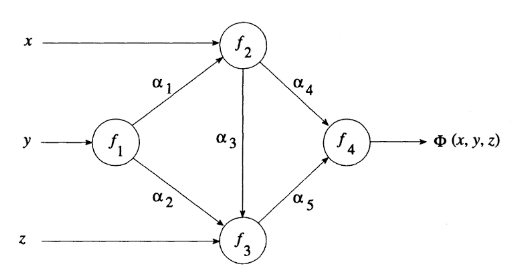
\includegraphics{NeuralNetworkExample.PNG}
		\caption{An example of a neural network consisting of neurons (Figure 
			\ref{fig:NeurEx}).  \cite{rojas2013neural}}
		\label{fig:NeurNetEx}
	\end{figure}
	
	% Neural Networks layers
	These created networks are divided in layers. The first layer is the 
	collection of all neurons that have an external input value. The last layer 
	is the collection of all neurons that generate output values. All layers in 
	between are called hidden layers, as a user cannot see those neurons from 
	the outside. \cite{Wang2003}
	
	% Training neural networks
	As explained in the section about machine learning, the neural network must 
	be trained (Section \ref{subsec:MachineLearning}). This can be done after 
	the architecture is defined. Again, with the data, a training and a test 
	set must be made, as well. With those, the neural network can be properly 
	trained to create the right output when giving values as an input. 
	 \cite{Wang2003}
	
	\subsubsection{Convolutional Neural Networks}
	
	% Introduction Convolutional Networks
	A more specific variant of neural networks is a convolutional neural 
	network (CNN). CNNs combine neural networks and convolutions to reduce 
	noise in the signal and approximate the actual input better. Convolutions 
	use kernels to use the values close to the input it wants to approximate. 
	It also uses pooling, which makes the input smaller by approximating a 
	location and its nearby inputs into one.  \cite{Goodfellow-et-al-2016}
	
	\clearpage
	
	\subsection{Deep Learning Frameworks}
	
	% Introduction Deep Learning frameworks
	A wide selection of deep learning frameworks are available. Most of these 
	frameworks are implemented in \textit{Python}, with some exceptions. A selection of 
	the five most popular are explained, together with their advantages and 
	disadvantages.
	
	\subsubsection{Scikit-learn Python}
	
	% Introduction Scikit-learn
	\textit{Python} itself has a package that can be used for machine learning, named 
	Scikit-learn. It is high-level interactive and is maturing in a quick rate, 
	due to its usage in both the academic world as in the industry. It also has 
	some C++ libraries incorporated, but makes most use of the three packages 
	\textit{NumPy}, \textit{SciPy} and \textit{Cython}. Due to his high-level and ease of use, a drawback 
	is its computational efficiency and therefore is not the best choice for 
	testing large data sets. \cite{pedregosa2011scikit}
	
	\subsubsection{Theano}
	
	% Introduction Theano
	\textit{Theano} is one of the open source machine learning frameworks written in 
	\textit{Python}. \cite{bergstra2010theano} Its programming is declarative. 
	 \cite{rampasek2016tensorflow} This one uses the famous \textit{NumPy} syntax for 
	higher computation speed 
	in its language. It was developed mainly to simplify the implementation of 
	the the algorithms used for well performing machine learning. Two tasks 
	that are intensive for the processor, either training a multi-layer neural 
	or a convolutional network. \textit{Theano} works through a pipeline on compilation 
	(Figure \ref{fig:TheanoPipe}). At first it puts the graph in standard form 
	(Canonicalization). Next it improves the stability of the computation 
	(stabilization). Thirdly it replaces expressions with faster ones 
	(Specialization). Fourth it moves the computation to the GPU, if compiled 
	for GPU (GPU transfer). In the last step it loads \textit{Python} modules with 
	specialized implementations (Code Generation).  \cite{bergstra2010theano}
	
	\begin{figure}[h!]
		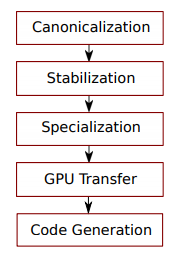
\includegraphics{TheanoPipeline.PNG}
		\caption{The steps \textit{Theano} takes in compilation for functions for GPU. 
			 \cite{bergstra2010theano}}
		\label{fig:TheanoPipe}
	\end{figure}
	
	% Theano extensions
	\textit{Theano} has been seen as a base for many other neural network creation 
	frameworks. Examples are \textit{Keras}, \textit{Lasagne}, \textit{GroundHog}, \textit{Blocks} and \textit{Pylearn2}. It 
	utilizes from the benefits of being written in \textit{Python}, such as creating a 
	friendly environment for fast and easy interaction with data. However, since 
	threading is done by \textit{Python}, it is not possible to have multiple 
	interpreters going on at the same time. The graph optimization time, code 
	compilation and memory usage time all can be improved.  \cite{al2016theano}
	
	\subsubsection{TensorFlow}
	
	% Introduction TensorFlow
	TensorFlow, also open sourced, is developed for experimentation on new 
	models, training those models with the help of large datasets and at last 
	move those models into production. \cite{abadi2016tensorflow} \textit{TensorFlow} 
	is 
	declarative and made in C++, while also having interfaces in \textit{Python}. 
	 \cite{rampasek2016tensorflow} Google makes regular use of \textit{TensorFlow}, 
	as an example. However many more programmers use TensorFlow for their 
	applications. It is a follow-up of the earlier system \textit{DistBelief} and 
	simplified and generalized that. \textit{TensorFlow} is mainly supporting training 
	and inference on a larger scale. It uses a data flow graph for representing 
	the computation within the algorithm and the operation state of the 
	algorithm.  \cite{abadi2016tensorflow}
	
	% Phases TensorFlow
	While executing a \textit{TensorFlow} application, two different phases can be 
	distinguished. The first phase of the two makes a to be trained neural 
	network and the update rules in the form of a data flow graph. The places 
	for input are reserved by place holders for state representation. The 
	second phase is the earlier neural network after optimization. Because of 
	these two phases, the execution phase can be optimized with the information 
	of the computation. There will not be any intermediate results slowing down 
	the process.  \cite{abadi2016tensorflow}
	
	Not only \textit{Theano}, but \textit{TensorFlow} as well has some wrappers, too. \textit{Keras} (also 
	for \textit{Theano}) and \textit{Pretty Tensor} both use \textit{TensorFlow} as a base for creating 
	neural networks.  \cite{rampasek2016tensorflow}
	
	\subsubsection{Caffe}
	
	% Introduction Caffe
	\textit{Caffe} is a framework based on the \textit{C++} library together with \textit{Python} and 
	\textit{MATLAB}. \textit{Caffe}, too, is open sourced and its programming is imperative. 
	 \cite{rampasek2016tensorflow} It is very useful for researches as 
	its code is modular and its network definitions are well separated. The 
	test coverage of \textit{Caffe} is useful as well, as every new module has a test 
	and is not accepted without a test. The bindings with \textit{Python} and \textit{MATLAB }
	makes constructing networks and classifying inputs easier. At last does 
	\textit{Caffe} provide pre-trained reference models. This makes it easier to 
	reproduce research.
	 \cite{DBLP:journals/corr/JiaSDKLGGD14}
	
	\subsubsection{Torch}
	
	% Introduction Torch
	\textit{Torch} is an object-oriented framework for machine learning and is 
	implemented in \textit{Lua}, but also has interfaces in \textit{C}. \textit{Torch} is also 
	imperative. \cite{rampasek2016tensorflow} A modular strategy was used to 
	simplify any 
	modifications of existing algorithms. There are four classes chosen. The 
	first class is about data handling (\textit{DataSet}). The second one is the black 
	box that gives an output (\textit{Machine}). The third is the class that is used to 
	find the optimal set of parameters (\textit{Trainer}). The last one is about 
	printing the measures of interest (\textit{Measurer}). These classes give a very 
	clear general idea. Several examples of usable machines are the gradient 
	machines, support vector machines and distributions. 
	 \cite{collobert2002torch}
	
	\subsubsection{Comparing Frameworks}
	
	% Kovalev comparisons
	Kovalev compared the likings of \textit{Theano} (with \textit{Keras} extension), \textit{Torch}, 
	\textit{Caffe}, \textit{TensorFlow} and the not discussed \textit{Deeplearning4J} based on convergence 
	and prediction time, classification accuracy and framework complexity 
	(lines of code). Both the depth (number of internal layers) and the width 
	(number of neurons within fixed number of layers). When regarding training, 
	prediction and testing times, all but \textit{Deeplearning4J} were performing quite 
	well. When watching Classification accuracy, \textit{Torch} and \textit{TensorFlow} performed 
	visibly unstable and \textit{Caffe} seemed to be a bit worse overall. The last 
	comparison, framework complexity was best for \textit{Theano}, followed by 
	\textit{TensorFlow} and then \textit{Caffe}. From best to worst the article rated the 
	following order: Theano (with \textit{Keras}), \textit{TensorFlow},\textit{ Caffe}, \textit{Torch}, 
	\textit{Deeplearning4J}.	 \cite{kovalev2016deep}
	
	% Caffe comparisons
	The creator of\textit{ Caffe} compared its own framework with other known 
	frameworks. The focus was mainly on basic parts of the programs, namely BSD 
	licence, core and binding languages CPU and GPU coverage, Open source, 
	training and the availability of pre-trained models. \textit{Caffe} has the advantage 
	in comparison with the earlier described \textit{Theano} and \textit{Torch} regarding binding 
	languages and the availability of pre-trained 
	models. \cite{DBLP:journals/corr/JiaSDKLGGD14}
	
	\begin{figure}[h!]
		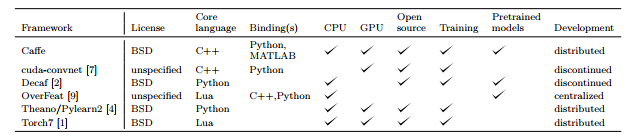
\includegraphics{CaffeMachineLearningComparisons.PNG}
		\caption{The comparisons between different machine learning frameworks 
			from \textit{Caffe} creator point of view. 
			 \cite{DBLP:journals/corr/JiaSDKLGGD14}}
		\label{fig:CaffeMachLearnComp}
	\end{figure}
	
	% Bahrampour's comparisons
	Bahrampour tested \textit{Caffe}, \textit{Theano},\textit{ Torch} and the not discussed \textit{Neon} on their 
	extensibility, hardware utilisation and speed for both CPU and GPU usage. 
	He stated that \textit{Caffe}, \textit{Theano} and \textit{Torch} were at that moment the top three 
	well developed and used frameworks. \textit{Neon} was added because of its 
	potential. The speed was measured by a forward time (check time it takes 
	for a pre-selected batch) and a gradient computation time (time for each 
	measurable parameter). The conclusion of the research had six parts: \textit{Theano} 
	and then \textit{Torch} are the most extensible. For both CPU- and GPU-based 
	training and deployment \textit{Theano} and \textit{Torch} are fighting for the number one 
	spot.\textit{ Torch} would benefit from expansion in both documentation and 
	debugging, though.  \cite{bahrampour2016comparative}
	
	% Chi's comparisons
	Another research that compared deep learning framework was Shi. The 
	frameworks \textit{Caffe}, \textit{TensorFlow} and \textit{Torch} were tested by him, as well as the 
	not discussed \textit{CNTK} from Microsoft and \textit{MXNet}. The tests that were done about 
	speed were on CPUs, one GPU and multiple GPUs on both synthetic and real 
	data. The overall outcome was that \textit{Caffe}, \textit{CNTK} and \textit{MXNet} performed better 
	than \textit{TensorFlow} and \textit{Torch}, although \textit{TensorFlow}'s production ramped up with 
	more threads.
	 \cite{DBLP:journals/corr/ShiWXC16}
	
	
	% Fox's comparisons
	Similar to Bahrampour \cite{bahrampour2016comparative}, Fox compared 
	\textit{TensorFlow}, \textit{Caffe},\textit{ Theano}, \textit{Torch} and the not discussed \textit{CNTK}, 
	\textit{Deeplearning4j}, \textit{MXNet} and\textit{ H2O}, for them being open-source, relatively 
	mature and adopted by the community. He mainly discussed the different 
	frameworks and afterwards made a table with all those findings (Figure 
	\ref{fig:FramewComps}).  \cite{fox2016software}
	
	\begin{figure}[h!]
		\includegraphics[scale=0.8]{FrameworkComparisons.PNG}
		\caption{Comparisons of eight frameworks. The comparisons were 
			implementation based.}
		\label{fig:FramewComps}
	\end{figure}
	
	% Parvat's comparisons
	Parvat had a more listings approach in comparing the frameworks \textit{Theano}, 
	\textit{Caffe}, \textit{Torch},\textit{ TensorFlow} and the not discussed \textit{Deeplearning4J} and \textit{NVIDIA cuDNN}. This time they were compared on their platform, interface, modelling 
	capability, support for \textit{CUDA}, \textit{OpenMP}, \textit{OpenCL} and support for pre-trained 
	models. He concluded that \textit{TensorFlow} was very flexible, due to being more 
	than a deep learning framework. \textit{Theano} is very helpful for creating models 
	fast, especially with the libraries, and therefore \textit{TensorFlow} and \textit{Theano} 
	are the most flexible. Torch is good because of the pre-trained models, 
	however misses being written in a mainstream language. \textit{Caffe} is useful when 
	working with images, and also has a lot of pre-trained CNN models. 
	\textit{Deeplearning4j} has its advantage being the only one working with \textit{Java} and 
	\textit{Scala}. 
	At last \textit{TensorFlow} has the advantage of being able to work with a 
	distributed environment.  \cite{parvat2017survey}
	
	A last article to discuss about comparing deep learning frameworks is 
	written by Erickson. Erickson focused on language, environment, speed and 
	maturity. \textit{Caffe}, being the most mature one and very fast, has a 
	disadvantage when tuning hyperparameters. \textit{TensorFlow} is regarded as hard 
	to use directly, however has good performance and tools for help. \textit{Theano} 
	is similar as \textit{TensorFlow}, in that it has good performance, however is a 
	bit harder to learn. Both of these frameworks can be made more user 
	friendly with a library as \textit{Keras}. \textit{Keras }uses the performance of either 
	\textit{TensorFlow} or \textit{Theano }and can be used easily to create models with 
	efficient code. Also \textit{Torch} is given a good maturity level and good 
	documentation.  \cite{erickson2017toolkits}
	
	% Final conclusions
	As can be seen by the many articles written about these frameworks, there is not a clear distribution as to which framework should be used when. It seems that \textit{Theano} and\textit{ TensorFlow}, especially with help from libraries such as \textit{Keras} are regarded a bit better than the others. On the other hand \textit{Caffe }
	has some advantages, too.
	
	
	
	
	\chapter{Case Study 1 - Bariatric Co-morbidities}
	\label{app:CS1}
	
	\section{Introduction}
	\label{sec:Intro}
	
	% Introduction Deneer's project
	The number of bariatric surgeries is increasing. worldwide. Although initially thought otherwise, this type of surgery has added benefits on top of losing weight. Among those benefits the remission of metabolic co-morbidities can be named. Due to binary labelling of those co-morbidities, valuable information is lost. On top of that the labelling is not clearly defined either. To obtain more and better results, this binary labelling could be replaced by a continuous severity score. Ruben Deneer conducted a research on trying to achieve a successful replacement.
	
	% First explanation data set
	The available data used for the research stemmed from the Catharina Hospital in Eindhoven (Subsection \ref{subsec:DataSets}). This extensive data set was a combination of two data sets and consisted of 41 markers measured pre- and post-surgery for 2367 patients that underwent gastric sleeve or gastric bypass surgery. These 41 markers are divided in several sub-panels that each describe different processes in the body. Conditions for these co-morbidities that were tested for the severity score were type II diabetes mellitus (T2DM), hypertension and dyslipidemia. Extensive literature research was done to connect them with 41 markers to find possible relations (Subsection \ref{subsec:CoMorMarkRel}).
	
	% The goal of the research
	To better specify the research on the data, a main goal was created: \emph{to use data mining techniques to develop score that can objectively quantify the severity of co-morbidities present in bariatric patients based on biomarkers, both before and after surgery.} \cite{Deneer2017Thesis} This means that it is not the goal to predict the outcome of the two types of surgery, but it is to quantify the improvement of the co-morbidities before and after the surgery.
	
	% Layout Report
	Since the data is not available other than within the hospital, a second research is proposed to complement Ruben Deneer's. The creation of this research consists of four parts. The first part was creating a research question, hypothesis and an own analysis approach without the knowledge of Deneer's (section \ref{sec:FirstProposal}). Since no data is available, this can only be made globally. It should be detailed enough to compare it with Deneer's own approach, though. Secondly a summary is given what was done in Deneer's research (section \ref{sec:OriginalResearch}). Thirdly the two are compared and remarks are given on the original approach (section \ref{sec:ProposalComparisons}). At last both are combined to create a final proposal for a possible follow-up research (section \ref{sec:FinalProposal}). 
	
	% Reference to Deneer's thesis
	Over the course of this proposal report, many references are made to the thesis of Ruben Deneer. These will not always be included for redundancy. Only when things are directly quoted from the thesis, a reference will be placed. Examples would be tables or goals.
	
	\subsection{Data Sets}
	\label{subsec:DataSets}
	
	% Introduction + first data set
	Two data sets were used in the study. The first one is called "The Dutch Audit for Treatment of Obesity" (DATO). This data set is a national database that houses all registrations and health statuses of pre- and post treatment bariatric surgery patients in the Netherlands. Several basic variables are noted, such as height, weight, BMI and date. Before surgery, the co-morbidities T2DM, hypertension and dyslipidemia were given a binary label of "Yes/No". After surgery they were given one of the following labels:
	
	\begin{enumerate}
		\item \textbf{Cured} No co-morbidity any more		
		\item \textbf{Improved} Less affected by co-morbidity
		\item \textbf{Same} No change in co-morbidity status
		\item \textbf{Worse} More affected by co-morbidity
		\item \textbf{Denovo} Diagnosed co-morbidity while not present before surgery
		\item \textbf{Not present} No co-morbidity present				
	\end{enumerate}
	
	% Second data set
	The second data set came from a laboratory database, stored in health records. This extensive data set consisted of 3 clinical and 38 blood markers measured pre- and 6, 12 and 24 months post-surgery. The tests pre-surgery had some additional markers on top of the 41 ones. These markers can be divided in the following categories: (Table \ref{tab:DataMarkers}) Complete blood count, liver function, kidney function, inflammation, lipid spectrum, coagulation, glucose metabolism, thyroid function and at last minerals and vitamins. The data sets of the patients that underwent bariatric surgery can be extracted from these. 
	
	\begin{table}
		\label{tab:DataMarkers}
		\caption{The markers present in the bariatric laboratory data set  \cite{Deneer2017Thesis}}
		\begin{tabular}{lll}
			\hline
			~                     & Before Surgery/Pre-Op/Screening                                                                                                                     & After Surgery/Post-Op/Follow-up                                                                                                                     \\ \hline
			Complete blood count  & \makecell{hemoglobin\\hematocrit\\erythrocytes\\mean corpuscular hemoglobin\\mean corpuscular volume\\thrombocytes\\leukocytes}                                & \makecell{hemoglobin\\hematocrit\\erythrocytes\\mean corpuscular hemoglobin\\mean corpuscular volume\\thrombocytes\\leukocytes}                                \\ \hline
			Liver function        & \makecell{bilirubin\\aspartate aminotransferase\\alanine aminotransferase\\lactate dehydrogenase\\alkaline phosphatase\\gamma-glutamyltransferase}             & \makecell{bilirubin\\aspartate aminotransferase\\alanine aminotransferase\\lactate dehydrogenase\\alkaline phosphatase\\gamma-glutamyltransferase}             \\ \hline
			Kidney function       & \makecell{urea\\creatinine\\potassium\\sodium\\calcium\\phosphate\\albumin}                                                                                    & \makecell{urea\\creatinine\\potassium\\sodium\\calcium\\phosphate\\albumin}                                                                                    \\ \hline
			Inflammation          & \makecell{C-reactive protein}                                                                                                                                  & \makecell{C-reactive protein}                                                                                                                                   \\ \hline
			Lipid spectrum        &  \makecell{total cholesterol\\high-density lipoprotein-cholesterol\\total/high-density cholesterol ratio \\low-density lipoprotein-cholesterol \\triglycerides} & \makecell{total cholesterol\\high-density lipoprotein-cholesterol\\total/high-density cholesterol ratio \\low-density lipoprotein-cholesterol \\triglycerides} \\ \hline
			Coagulation           & \makecell{prothrombin time}                                                                                                                                    & \makecell{prothrombin time}                                                                                                                                   \\ \hline
			Glucose metabolism    & \makecell{hemoglobin A1c (IFCC)\\glucose\\insulin\\C-peptide}                                                                                                  & \makecell{hemoglobin A1c (IFCC)\\glucose\\-\\-}                                                                                                                \\ \hline
			Thyroid function      & \makecell{parathyroid hormone\\thyroid-stimulating hormone\\free T4\\cortisol}                                                                                 & \makecell{parathyroid hormone\\-\\-\\-}                                                                                                                        \\ \hline
			Minerals and vitamins & \makecell{iron\\ferritin\\folic acid\\zinc\\magnesium\\vitamin A\\vitamin B1\\vitamin B6\\25-OH vitamin D\\vitamin B12}                                        & \makecell{iron\\ferritin\\folic acid\\-\\-\\-\\vitamin B1\\vitamin B6\\25-OH vitamin D\\vitamin B12}                                                           \\ \hline
		\end{tabular}
	\end{table}
	
	% Data combining challenge one
	One part of the research is to combine these two data sets. Some challenges arise when doing so. Such a challenge is obviously to find the right connection between them, using the survey and lab data of the same patient. These challenges must be solved before asking the question what markers can say about the severity of co-morbidities.
	
	% Data driven challenge two
	A second challenge would be to define what must be done with non-matching data. Pre-treatment for example more markers were used than post-treatment. These missing ones might be more useful for scoring the co-morbidity severity than the known markers. There also might be measurements that were missing or corrupted, whereas other markers might still be useful enough for a result. How to tackle this missing data challenge should be defined properly.
	
	\subsection{Co-morbidity Marker Relation}
	\label{subsec:CoMorMarkRel}
	
	% Introduction section
	For some of the markers it is clear they affect the severity score of a co-morbidity. Co-morbidity is diagnosed from these markers and therefore a relation is imminent. For others more subtle relations are present, that in first sight would not be recognised. Both are important for assigning a co-morbidity severity score.
	
	% Clear relations
	All three co-morbidities can be derived from specific markers. T2DM is known for higher glucose and insulin levels in the blood, while hardly finding any C-peptides. Ideally these would be used to find T2DM, however these values vary significantly over the day. Therefore help from other markers should be helpful. Hypertension is best measured with blood pressure measurements (BP). These however are not reliable for the nervous patients in the hospital and other markers must be found for help. Thirdly dyslipidemia obviously can be found using markers in the lipid spectrum (Table \ref{tab:DataMarkers}), however there may be other markers contributing to dyslipidemia detection, as well.
	
	% Less well-known relations
	For T2DM, hypertension and to a lesser extend dyslipidemia, more knowledge on relations between them and markers would benefit the creation of a severity score. Literature research is done to understand more of those subtle relations and know that those exist when trying to create a morbidity score. The outcome of this literature search shows that quite some relations can be found between co-morbidities and the markers (Table \ref{tab:CoMorMarkRel}). For most it is definitely worth to investigate any relation.
	
	\begin{table}[]
		\centering
		\caption{Relations found in literature between the co-morbidities and markers. \cite{Deneer2017Thesis}. The number shows how many citations were found that state a relation exist, nothing means no relation. A 'D' means that the disease is diagnosed from those markers.}
		\label{tab:CoMorMarkRel}
		\begin{tabular}{llll}
			\hline
			& \textbf{Diabetes} & \textbf{Hypertension} & \textbf{Dyslipidemia} \\ \hline
			hemoglobin            & 3                 & 1                     &                       \\
			hematocrit            & 2                 & 2                     &                       \\
			erythrocytes          & 1                 & 1                     &                       \\
			MCH                   &                   & 1                     &                       \\
			MCV                   &                   & 1                     &                       \\
			thrombocytes          &                   &                       &                       \\
			leukocytes            & 4                 & 3                     & 1                     \\
			bilirubin             & 3                 & 1                     & 1                     \\
			ASAT                  & 1                 & 1                     & 1                     \\
			ALAT                  & 4                 & 1                     & 1                     \\
			LD                    & 1                 &                       &                       \\
			Alkaline phospatae    & 2                 &                       &                       \\
			gamma GT              & 4                 & 2                     & 1                     \\
			urea                  & 1                 & 3                     &                       \\
			creatinine            &                   & 2                     & 1                     \\
			potassium             &                   & 2                     &                       \\
			sodium                &                   & 1                     &                       \\
			calcium               & 2                 & 1                     & 1                     \\
			phosphate             &                   &                       &                       \\
			albumin               &                   &                       &                       \\
			CRP                   & 3                 & 4                     & 1                     \\
			cholesterol           &                   & 2                     & D                     \\
			HDL-cholesterol       &                   & 2                     & D                     \\
			chol/HDL ratio        &                   &                       & D                     \\
			LDL-cholesterol       &                   & 2                     & D                     \\
			triglycerides         &                   & 2                     & D                     \\
			prothrombin time      &                   &                       &                       \\
			hemoglobin A1c (IFCC) & D                 &                       &                       \\
			glucose               & D                 & 2                     &                       \\
			parathormone          & 1                 & 2                     &                       \\
			iron                  &                   &                       &                       \\
			ferritin              & 3                 & 1                     & 1                     \\ \hline
		\end{tabular}
	\end{table}
	
	\clearpage
	
	\section{First Proposal}
	\label{sec:FirstProposal}
	
	% Research question
	To start of a research proposal, the first thing that needs to be done is to create a research question that fits the intended goal. This main question can then be divided in several sub questions for explaining the steps how to answer it. Next hypotheses should be made for the main and sub questions. Third and last the methods of how to answer the research questions are discussed. Since this is only a first proposal, the methods part will be limited, and extended in future proposals.
	
	\subsection{Research Questions}
	
	% Main question
	As stated earlier (Section \ref{sec:Intro}) the goal was to develop a severity score for the co-morbidities using data mining. A research question for this goal would then be:
	
	\begin{enumerate}
		\item[] \emph{Can a severity score for co-morbidities present in bariatric patients based on biomarkers be developed?}
	\end{enumerate}
	
	% First sub-question
	This main research question includes all aspects of the goal. It should be specified in several different sub-questions ot make it clearer. A first sub-question could be about the relation between co-morbidities and biomarkers, which is a major part on making this score.
	
	\begin{enumerate}
		\item \emph{Which relations are present between co-morbidities and the biomarkers?}
	\end{enumerate}
	
	% Second sub-question
	A second sub-question should be about retrieving a score for the co-morbidities from the biomarkers. This score retrieval should use the outcome of the first sub-question to efficiently find the correct score.
	
	\begin{enumerate}[resume]
		\item \emph{How can a severity score of co-morbidities be obtained from biomarkers?}
	\end{enumerate}
	
	% Explanation relation both questions to main
	This second question mainly focuses on techniques to achieve a sufficient answer to the main research question. When both sub-questions are sufficiently answered, then the main one should definitely be, as well.
	
	\subsection{Hypothesis}
	
	% Pre-conditions
	The data set available for this research is quite extensive. The number of biomarkers is high, there are many relations between them, co-morbidities are known and a high number of patients has been tested for both. These pre-conditions are very beneficial to finding positive answers for the research questions.
	
	% First sub-question
	Knowing many relations between the co-morbidities and biomarkers beforehand implies that a lot of them should be present in the data set. to the first sub-question which relations are present, the answer would be two-fold. First strong relations between the co-morbidities and on the other hand biomarkers that help diagnosing them are expected. This would for example be the case for dyslipidemia and biomarkers of the lipid spectrum. Weaker relations are expected for all found in literature (Table \ref{tab:CoMorMarkRel}).
	
	% Second sub-question
	As for the second sub-question how a score can be defined from biomarkers, several different options are possible. When knowing there is a relation between biomarkers and the co-morbidity, by machine learning combined with regression a function can be made predicting a score outcome for the biomarkers. This score is then compared with the categorical labelling of co-morbidities to find out if they match. Through training the model and afterwards testing it, the score is validated. 
	
	% Main research question
	With the hypotheses for both sub-questions the main research question can be answered, too. The hypothesis for this one would be that it is possible to find a severity score with the biomarkers. A model can made using the biomarkers as an input and retrieving a severity score as output.
	
	\subsection{Methods}
	
	% Materials
	Since the materials are all explained in Deneer's thesis, that part and most of the pre-processing is skipped in methods. One thing that needs to be discussed is the handling of markers that are measured pre-surgery, but not post-surgery. These could be removed as being redundant. They may, however show a significant difference between availability or absence of a co-morbidity. This is a vital result for possible further bariatric surgeries and co-morbidity scoring. Therefore at least some tests should be done with those pre-surgery biomarkers. For post-surgery measurements they can be removed from the tests or they can be given a dummy value as being unknown.
	
	% Methods first sub-question
	The first research question can be easily and efficiently answered with statistical analysis. This approach can be used to compare two groups of values, whether the co-morbidity is present or not. Since for this question a score is not yet needed, dividing the patients between having a co-morbidity or not suffices. The markers that show a significant difference in mean or variance should be noted and given extra care in future researching to create a score. Aside from comparing original measurements of the markers, combinations between them should be tested for statistical analysis as well. Some are already present, for example the \textit{cholesterol / HDL-cholesterol ratio}. There may be more interesting combinations that could show a significant difference for either of the three co-morbidities.
	
	% Program first sub-question
	Since the data needs some manipulation to find those markers that are significantly different for presence or absence of co-morbidities, a more advanced statistical program that can do those manipulation would be best to use. This means that the best choices would be \textit{R}, \textit{MATLAB} or \textit{Python}. \textit{Python} with \textit{SciPy} was chosen of those three for also being a good choice for researching the second sub-question and because the actual users knows \textit{Python} quite well. The outcome of this research can most likely immediately used in the second one for the next sub-question
	
	% Program second sub-question
	The second research question is a bit more complex to answer. The quickest one is to use a way of machine learning to create this score. Some sort of regression is the first thing that comes to mind and simple support vector machines (SVMs) seem to be a good way to start. However obtaining a continuous score from categorical, or in the case of pre-surgery even binary, labels. A score interval needs to be set up and these binary or categorical values should be translated to a certain score on the interval. The way to score these values can be proposed, but most likely needs more insight to find out what is best. At first just a categorical learning system seems best. Both a selection of from sub-question resulting useful markers should be used as well as the complete set to find a good score.
	
	% At the start a score interval of 0\% to 100\% will be chosen, with 0\%-50\% being not having the disease and 50\%-100\% having it, with different severities. Binary cases will then be given 25\% and 75\% as absent and present co-morbidity respectively, knowing those as the values they should be closest to. The ordinal cases that showed improvement or deterioration will be given a score of 50\%. 
	
	% Program second sub-question
	At the start of researching the second sub-question a standard machine learning framework would suffice. This means that the aforementioned \textit{Python} with the \textit{scikit-learn} package would be best to start with. When initial results indicate that a certain way of handling this data in another way would be more efficient, \textit{Python} is used by many other machine learning programs, such as Theano, TensorFlow and both their packages. Therefore \textit{Python} would be a great way to start the project of which the direction can change heavily.
	
	\clearpage
	
	\section{Original research}
	\label{sec:OriginalResearch}
	
	% Introduction original research
	Now that an initial proposal is made, the original research should be discussed. The research is divided into two parts. The first is all about the material and how this was preprocessed. The second part focused more on modelling using the data sets. Multiple approaches have been used to show different aspects of the data.
	
	\subsection{Preprocessing}
	\label{subsec:Preprocessing}
	
	% Merging data sets
	As discussed earlier (subsection \ref{subsec:DataSets}), the data was retrieved from two data sets, the DATO and lab set. These two were not perfectly lined up and therefore merging those required some specific rules. At first, any entries that were double on the same date were removed if having conflicting information. Entries that had surgery before 2012 were removed, too, due to not having a pre-screening test. Secondly all DATO and lab sets were paired up if they did not have more than 90 days between them. When double matches occurred, the closest ones were taken. Also only pairs were taken when they were on one of the four periods (pre-, 6, 12 or 24 post-surgery) and others were omitted.
	
	% After merging preprocessing
	After merging both data sets the lab data was prone to preprocessing. Ten biomarkers were dropped from the set, due to missing values. Five (Zinc, vitamin A, free T5, methylmalonic acid, LDL) were dropped due to severe missing data or explanations by other data. Five others (TSH, insulin, C-peptide, magnesium and cortisol) were dropped due to only being available in pre-surgery screening. CRP was dichomotized, due to being truncated and other variables were changed to their cut-off value when only a small portion of them was truncated, too. Inconsistencies in DATO meant that the patient would be dropped. After all these markers were being removed, a total of 60 variables were present in the data set (figure \ref{fig:FinVar}) and a number of 2367 patients with a 2.35 of data sets per patient on average (figure \ref{fig:FinPat}). The number of variables used for modelling was reduced to 49. From those, a number of variables were removed again. Weight and height (incorporated in BMI), vitamins (were supplemented), iron (variation too high), year, type of and months before/after surgery (no value, or found elsewhere) were all removed. Furthermore Creatinine was replaced by glomerular filtration rate (GFR), the ASAT/ALAT ratio was added, the prothrombin time (PT) was replaced by the international normalized ratio (INR) and at last calcium was corrected by adding an albumin factor. 
	
	\begin{figure}
		\includegraphics[scale=0.8]{FinalVariables.PNG}
		\label{fig:FinVar}
		\caption{All variables present after pre-processing  \cite{Deneer2017Thesis}}
	\end{figure}
	
	\begin{figure}
		\includegraphics[scale=0.8]{FinalPAtients.PNG}
		\label{fig:FinPat}
		\caption{All patients present after pre-processing  \cite{Deneer2017Thesis}}
	\end{figure}
	
	\subsection{Modelling}
	
	% Modelling layout
	After preprocessing the data, a series of steps should be taken to create a sufficient model for the issue. First an ordinal outcome definition was made for scoring the co-morbidities. Next, statistical learning models were created, based on logistic regression and all aspects of this model were discussed to find, validate and visualize a correct model.
	
	% Ordinal outcome
	To make one scale for all co-morbidities a new ordinal outcome was created. This scoring was made with three different categories, being: no, one or multiple co-morbidities present. The choice for this scoring was made with the idea that people with more co-morbidities also had a higher severity compared with patients that had less or none. The multiple co-morbidities category was a merge from having two and three, in order to make the categories more balanced in size. This way none has most patients (1329) and one and multiple still had a high enough number (569 and 469 respectively). 
	
	% Statistical models
	To create a model in this research, a classification method should be used. A well known one for that was logistic regression. Maximum likelihood estimation was used to estimate regression coefficients for the variables. Multicollinearity had to be limited as much as possible, as it was assumed to be absent for logistic regression. A correlation matrix was created to find multicollinearity. Special interactions were included as well, for example the Body mass index (BMI) and presence for co-morbidities as being a prerequisite for the surgery. For ordinal outcomes of the logistic regression, both proportional odds (PO) and continuation ratio (CR) were used. 10-fold cross validation was done to validate the model and an assessment of model fit was done for discrimination, calibration and overall performance. Lastly the model was visualized with a nomogram for further use.
	
	\clearpage
	
	\section{Proposal Comparisons}
	\label{sec:ProposalComparisons}
	
	% Introduction proposal comparisons
	A proposal was created after reading the introduction, background and material. The original research was also discussed and a summary was given. The new proposal should now be compared with the original research to find out when they match and when they do not. Several topics should be discussed that differ greatly between the original and new proposal. These differences should be addressed to create a final proposal for a new research. The first difference was about data omission. Many aspects of the original data set were debatable whether they should be removed or not. A second difference was the final scoring system. The newly proposed one was vastly different from the original one.
	
	\subsection{Data Omission}
	
	% Data omission locations
	In preprocessing (subsection \ref{subsec:Preprocessing}) a big number of data omissions was done with various reasons. While many of them were regarded as valid, a number of them could be seen as being a bit too rigorous. These questionable ones were discussed whether they should be left out.
	
	\begin{enumerate}
		\item \textbf{Lab set without a close DATO set} Several lab sets were removed because no DATO set was close enough. This seemed logical as they should match for complete results. However the DATO set had many variables that are not subject to much change over time. If a lab set was squeezed in between DATO sets that were very similar, an estimate for the intermediate DATO set at that time could easily be made.
		
		\item \textbf{Predefined measuring moments} The DATO and lab sets were all measured on predefined moments. There were other times as well, though, were measurements took place. On those other times data was omitted. These omissions seemed too rigorous. These data sets were maybe not useful enough to show differences on those measuring moments, however these sets could be very helpful to create a model. These questionable omissions included pairs that were double at one moment and moments at 36 or 48 months. 
		
		\item \textbf{Markers only in pre-surgery measurements} Five of the biomarkers were only measured before surgery. The reason for this was not stated, however these markers were removed as about half of the data sets had these. When almost 50\% of the data sets had these markers, there was enough available to check these variables on their relation with the co-morbidities. If all of them showed no significant difference in presence or absence of the co-morbidities, then they were not useful. If they would show a significant difference, they might be a good marker for further co-morbidity detection. Disregarding them only because half of the sets did not have the value seemed questionable.
		
		\item \textbf{LDL-cholesterol} This marker from the lipid panel was removed due to its possible derivation from the same panel markers. The omission was discussed quite heavily in the thesis. Even though it was derived from other markers, the derivation was done in a very specific way. Maybe a description for one of the co-morbidities would benefit greatly of this specific derivation. Omitting LDL-cholesterol was less questionable than the other cases, however at least some tests could be done to check the significance.
		
	\end{enumerate}
	
	\subsection{Scoring System}
	
	% Difference scoring system
	At the project start a goal was made about creating a severity scoring system for co-morbidities. To achieve that from categorical data, as little data reduction as possible should be done to keep the score quality as high as possible. The proposed ordinal system however actually reduces information. First there is no distinction between two or three co-morbidities. The type of co-morbidity is removed, too, as well as its progress after surgery. This is a very counter intuitive way to correctly model a scoring system when these three decisions all could contribute to a more efficient scale.
	
	% Final scoring system
	A second remark about the scoring system is about the final product. The linear predictor score was not really an answer to the original goal. The goal was to create a severity score, whereas the linear predictor score in the nomogram is originated from its probability counterpart and not really showing severity. As discussed earlier, it was hard to create a severity score from categorical labelling, so maybe that goal might be too ambitious. %Using predictability score was a straightforward start for this, though, as those could be calculated. Further research could lead to a severity score from that. 
	
	% Better proposal
	For this research it seemed better to keep the three co-morbidities separate as long as possible. For every co-morbidity separately a score could be made which in the end could be joined together. This score would be best based on a probability at the start, so how much chance there was to have a certain co-morbidity. After creating probability models for all of them, they could be combined in a joint probability model. While doing this, obviously collinearity needed to be taken into account. As recently discussed, a probability model was not according to the goal. A score was desired and not a probability. Since the data was not gathered in a way to find a score with the measured tasks, this was much harder. After possibly finding good results for a probability model, a next step could be to translate that model in a scoring system.
	
	\subsection{Modelling Tools}
	
	% Used modelling tools
	About every part of the original research was done in R. As discussed previously, especially the variable significance could be done efficiently in R, as it was one of the more advanced tools to do statistical analysis with. For the modelling part however there were more advanced programs or frameworks that could be used. One of the reasons to choose R was to create a "white-box" answer, that every step of the process could be explained. The disadvantage in choosing a white-box model, however, was that the result could be worse than for a more traditional machine learning approach. Those approaches could lead to a better result and were therefore definitely worth to investigate. In R however, machine learning options were extremely limited if even available. Other programs or frameworks could facilitate that better than R, such as \textit{Python} with the Scikit-learn package, Theano or TensorFlow This could also facilitate a better final visualization result for the scoring system than the nomogram, which was not very user-friendly and straightforward.
	
	\clearpage
	
	\section{Final Proposal}
	\label{sec:FinalProposal}
	
	% Introduction final proposal
	The final proposal combined the first one and the original research for optimization. Questions from the first proposal were re-used, with some modifications and additions. The hypotheses were changed accordingly. The methods for answering the research questions were similar to the ones in the first proposal, however, they were extended after more information from the original research was added. 
	
	\subsection{Research Questions}
	
	% Main research question
	The main research question stayed the same as the one from the first proposal. This was the main goal of the research and therefore was a good all-encompassing question for it. 
	
	\begin{enumerate}
		\item[] \emph{Can a severity score for co-morbidities present in bariatric patients based on biomarkers be developed?}
	\end{enumerate}
	
	% First sub-question
	The first sub-question also stayed mostly the same. It was a bit unclear that there was relevant data in the DATO set. Therefore instead of saying biomarkers, the term "available variables" would be used. The word available was added due to not immediately omitting some of the variables, so their relation to co-morbidities would still investigated.
	
	\begin{enumerate}
		\item \emph{Which relations are present between co-morbidities and the available variables?}
	\end{enumerate}
	
	% Addition to first sub-question
	One thing the original research correctly investigated that was not thought of, was collinearity. This was already investigated for most variables, however the ones then removed might still have collinearity characteristics. Therefore a new sub-question was added to find those.
	
	\begin{enumerate}[resume]
		\item \emph{Which collinearity relations are present within the available variables?}
	\end{enumerate}
	
	% Second sub-question I
	The other sub-question was about adding a score to the co-morbidities originated from variables. This question was quite vague and with the help of the original research it was split up in three separate questions. The first one was about modelling the co-morbidities with variables.
	
	\begin{enumerate}[resume]
		\item \emph{How are the co-morbidities best modelled with the available variables?}
	\end{enumerate}
	
	% Second sub-question II
	The second part of the split sub-question was about the scoring part. Eventually a score should be given to the co-morbidities, which must be investigated thoroughly.
	
	\begin{enumerate}[resume]
		\item \emph{How can scores best be added to the available co-morbidity models?}
	\end{enumerate}
	
	% Second sub-question III
	The last part was about combining the co-morbidities together. Until now they were regarded separately, but the eventual result should have these scores combined. Therefore the third one of the split sub-question was about combining those.
	
	\begin{enumerate}[resume]
		\item \emph{How can the co-morbidity models best be combined?}
	\end{enumerate}
	
	% Final thoughts
	This main question and the five sub-question should cover all aspects in this research. If all questions were answered one by one, a scoring model for the co-morbidities should be available for bariatric patients.
	
	\subsection{Hypotheses}
	
	% Introduction Hypothesis
	Since three sub-questions are added. The new hypotheses should be added, as well. They will be addressed in order of appearance and afterwards a general hypothesis will be given for the main research question.
	
	% First sub-question
	The first sub-question has the same hypotheses as in the earlier proposal. Strong relations should be found in the markers that the co-morbidities are diagnosed from and weak relations should be found in the ones that are linked in literature. On top of that, since the original research answered this question partially, too, the following variables should show strong relations: triglycerides, HbA1c, CKD.EPI, age.at.surgery, HDL, cholesterol0-HDL-ratio, albumin, period, potassium, period * BMI, cholesterol and urea. All of these showed the best correlation.
	
	% Second sub-question
	The second sub-question has also been partially answered in the original research. Therefore strong relations should be found between: hematocrit and hemoglobin, MCV and MCH, ALAT and ASAT, HbA1c and glucose, hemoglobine and gender, erythrocytes and hematocrit. Aside from these mostly the omitted variables should show relations within their own panel. Insulin for example is expected to show a relation with glucose and C-peptide.
	
	% Third sub-question
	The third sub-question is partially answered in a specific direction by the original research. Logistic regression was extensively investigated, however other machine learning aspects were not used. The hypothesis is that most likely several machine learning methods should be sufficient to answer this question. With those machine learning methods a model can be derived for the co-morbidities to be found out of the available variables.
	
	% Fourth sub-question
	The fourth question is the also hardest. How can a score be added? The original research started first with an ordinal score, which is debatable for the information thrown away. When thinking ahead, the best idea for now is to start with a probability score. These probabilities usually also show the severity, as having a higher probability for a co-morbidity, the severity of it usually is bigger, too. After having a probability score further insights can be used to create a better score than probability. An example of such a score can be this:
	
	\begin{enumerate}
		\item[] \textbf{Score proposal} At the start a score interval of 0\% to 100\% will be chosen, with 0\%-50\% being not having the disease and 50\%-100\% having it, with different severities. Binary cases will then be given 25\% and 75\% as absent and present co-morbidity respectively, knowing those as the values they should be closest to. The ordinal cases that showed improvement or deterioration will be given a score of 50\%. 
	\end{enumerate}
	
	% Fifth sub-question
	The last sub-question is bigger than only adding them together. Since the co-morbidities are also related to each other, these correlations have to be taken into account when creating a score. On the other side, when two co-morbidities are both present in a patient, they also have a bigger chance to be more severe, as they strengthen each other. Different additions or combinations can be tested to combine them.
	
	% Main research question
	The hypotheses of most sub-questions are fairly straightforward and with the original research are known to give results already. The aim is however to create better answers than the already available ones. For the first two questions this is definitely possible, the last three depend whether the results will be improving the known ones already, mainly because it is a new area for researching. Still, though, as there is already one present, the main research question can be answered with a yes.
	
	\subsection{Methods}
	\label{subsec:FinalMethods}
	
	% Introduction methods
	This time the methods is changed a bit from the first proposal, as it would be better to line them up with the original research and show differences between those. So first preprocessing is started as well as everything related to that. Secondly the modelling part will be discussed, together with the sub-questions that are answered in here.
	
	% Preprocessing
	In preprocessing almost every thing will be done the same as in the original research. Most differences will be in not removing certain parts of the data set. This means that more than one data set can be made for the different instances. All differences will be discussed.
	
	\begin{enumerate}
		\item \textbf{All paired DATO and lab set} All data that is available after pairing the DATO and lab set will be put in a data set. There will not be any distinction between data on predefined moments and not, because for modelling those do not matter at all. In case more results should be generated only on those predefined moments, a separate attribute set will be made to extract those.
		
		\item \textbf{Variables omission} Not all variables will be omitted when a significant number of them is available. Relations between those variables and with the co-morbidities will be tested. When finding out that there are significant relations between them, possible further research will be done on both a set with and without them. Variables that fall into this category are the five that are only measured pre-surgery and LDL.
		
	\end{enumerate}
	
	% Modelling layout
	Several steps should be taken to achieve the final goal. First the variables needs to be compared with the co-morbidities (sub-question 1) and themselves (sub-question 2). Next a model has to be found (sub-question 3) for all co-morbidities as well as a score added to the model (sub-question 4). Lastly the three models need to be combined (sub-question 5) to create a final answer to the main research question.
	
	% Variable exploration
	To answer the first two sub-questions, statistical analysis must be done. Correlation matrices must be made to see whether two variables or one and a co-morbidity correlate significantly. Also the variables must be checked on their own population, whether they have a high variance and follow a statistical distribution. In case of high correlations between variables, a joint variable should be created if possible. At last, also combinations of variables should be created and tested for relations with co-morbidities. This all can efficiently be done in \textit{Python} with the \textit{SciPy} package.
	
	% Co-morbidity modelling
	A co-morbidity can be modelled using different approaches in machine learning. Several classification techniques are available such as support vector machines (SVM), nearest neighbour (NN), stochastic gradient descent (SGD). Research must be done which is most applicable and testing must be done which gives the best results. This is repeated three times for every co-morbidity. Within \textit{Python} the Scikit-learn package has the basics to create proper results and if needed, programs such as Theano or TensorFlow can be used within \textit{Python} for more extensive research. For testing, a similar approach as in the original result can be used, called 10 fold cross-validation. The final model and the visualisation depends on the type of machine learning used, however graphs that show clusters of morbidities for several variables seems a good way to approach that.
	
	% Co-morbidity scoring
	Scoring addition in machine learning approaches is a challenge. At first tests can be done with changing the methods from classification approach to their regression counterpart, for example from SVC (Support Vector Classification) to SVR (-Regression). This can have major for now unknown implications. As discussed earlier (subsection \ref{subsec:FinalMethods}) setting up a score interval should be thought of before and also able to be implemented. The proposed score can be used as a base and be changed if advantageous.
	
	% Co-morbidity combination
	The last challenge is to create a model that combines all three of the co-morbidities. To start this, all three separate models can be used to create the combination. If this does not give the desired results and makes scores much worse than initially thought, a similar ordinal system as used in the original approach can be used. Then sub-questions three and four are repeated only with co-morbidities combined, removing details from each different one.
	
	\chapter{Case Study 2 - Skin Diseases}
	\label{app:CS2}
	
	\section{Introduction}
	\label{sec:Introduction}
		
	% Explanation skin disease data
	To find out what techniques and guidelines are useful to put in a framework for biomedical engineers, a case study is done with an example biomedical dataset. This example dataset is a based on gene expression of skin diseases \cite{nair2009genome, suarez2012expanding, bigler2013cross, kim2016spectrum, yao2008type, suarez2011nonlesional, tintle2011reversal, gittler2012progressive} and is a microarray dataset. Two skin diseases were intended to be examined with this dataset, psoriasis and atopic dermatitis. The expression for a total of 54675 genes were measured for skin disease patients on skin affected by the disease (lesional skin) and skin not affected by the disease (non-lesional skin). Further data from healthy subjects was also acquired. Nine datasets were available, six for psoriasis \cite{nair2009genome, suarez2012expanding, bigler2013cross, kim2016spectrum, yao2008type} and three for atopic dermatitis \cite{suarez2011nonlesional, tintle2011reversal, gittler2012progressive}. The number of tested skin biopies ranged from 28 to 180 per dataset whereas the number of measured genes is the same for every set, namely 54675.
	
	% Explanation skin data analysis
	In this project, a basic analysis was done on the available skin disease datasets, as a case study for creating a framework for biomedical engineers. First, a background is given on the dataset. Secondly, methods to extract information from the data are explained, followed by their results. Finally, the results are discussed and useful aspects for a biomedical engineering framework about the basic analysis are concluded from the case study.
	
	
	\section{Skin Diseases Datasets}
	\label{sec:SkinDiseasesDataSet}
	
	% Introduction
	Skin diseases can have a major impact in someone's life. Whereas skin diseases are not as life threatening as diseases such as cancer, Alzheimer and AIDS, they can lower quality of life significantly. When looking at the health-related quality of life (HRQL), patients with psoriasis show the same problems as patients with other major chronic health conditions \cite{rapp1999psoriasis}. Patients with psoriasis or atopic dermatitis suffer from severe itching and pains. Further insights into the skin diseases can help alleviate their unwanted side-effects and help improve the patients' quality of life \cite{jowett1985skin}.
	
	% Dataset introduction
	Information on both of these skin diseases can be found in nine datasets stored on the NCBI database \cite{edgar2002gene}. The datasets comprise microarray data extracted biopsies of psoriasis patients, both from their lesional and non-lesional skin. In several experiments this skin is taken from the same patient. Also some skin is taken from patients not suffering from any of these two diseases. six datasets gathered data from Psoriasis patients and three from atopic dermatitis patients. These datasets consist of a total number of 54675 genes, the features of the dataset. The range of acquired samples varies among datasets from 28 tot 180. Also, since every dataset was created by different people, some minor differences can be present in them as well (Table \ref{tab:SkinDiseasesDataSets}), due to different measurement equipment.
	
	\begin{table}[h!]
		\centering
		\caption{Details of the nine skin disease datasets. The number of samples and genes has been given, as well as remarks of the skin types.}
		\label{tab:SkinDiseasesDataSets}
		\begin{tabular}{cc|ccl}
			\textbf{Disease}                                                     & \textbf{Dataset name} & \textbf{Number of samples} & \textbf{Genes} & \textbf{Sample size remarks}                                                                                                                                                                                                                                        \\ \hline
			\textbf{Psoriasis}                                                   & \textbf{GSE13355}  \cite{nair2009genome}      & 180                  & 54675             & \begin{tabular}[c]{@{}l@{}}Three skin types: \\ - NN (normal, 64 samples)\\ - PN  (non-lesional, 58 samples) \\ - PP (lesional, 58 samples)\end{tabular} \\ \cline{3-5} 
			\textbf{}                                                            & \textbf{GSE30999}  \cite{suarez2012expanding}      & 170                  & 54675             & \begin{tabular}[c]{@{}l@{}}- No normal patients\\ - Non-lesional (85 samples)\\ - Lesional (85 samples)\end{tabular}                                                                                                                    \\ \cline{3-5} 
			\textbf{}                                                            & \textbf{GSE34248}  \cite{bigler2013cross}      & 28                   & 54675             & \begin{tabular}[c]{@{}l@{}}- No normal patients\\ - Non-lesional (14 samples)\\ - Lesional (14 samples)\end{tabular}                                                                                                                              \\ \cline{3-5} 
			\textbf{}                                                            & \textbf{GSE41662}  \cite{bigler2013cross}      & 48                   & 54675             & \begin{tabular}[c]{@{}l@{}}- No normal patients\\ - Non-lesional (24 samples)\\ - Lesional (24 samples)\end{tabular}                                                                                                                               \\ \cline{3-5} 
			\textbf{}                                                            & \textbf{GSE78097}  \cite{kim2016spectrum}      & 33                   & 54675             & \begin{tabular}[c]{@{}l@{}}Different types of skin samples: \\ - Normal (6 samples)\\ - Mild Psoriasis (14 samples) \\ - Severe Psoriasis (13 samples)\end{tabular}                                                                                \\ \cline{3-5} 
			\textbf{}                                                            & \textbf{GSE14905}  \cite{yao2008type}     & 82                   & 54675             & \begin{tabular}[c]{@{}l@{}}- Normal skin (21 samples), \\ - Non-lesional skin (28 samples)\\ - Lesional skin (33 samples)\end{tabular}                                                                                                                 \\ \hline
			\textbf{\begin{tabular}[c]{@{}c@{}}Atopic\\ Dermatitis\end{tabular}} & \textbf{GSE32924}  \cite{suarez2011nonlesional}      & 33                   & 54675             & \begin{tabular}[c]{@{}l@{}}- Normal skin (8 samples) \\ - Non-lesional skin (12 samples)\\ - Lesional skin (13 samples)\end{tabular}                                                                                                         \\ \cline{3-5} 
			\textbf{}                                                            & \textbf{GSE27887}  \cite{tintle2011reversal}      & 35                   & 54675             & \begin{tabular}[c]{@{}l@{}}Different type of skin samples, \\ pre and post treatment of skin: \\ - Pre non-lesional (8 samples)\\ - Post non-lesional (9 samples)\\ - Pre lesional (9 samples)\\ - Post lesional (9 samples)\end{tabular}       \\ \cline{3-5} 
			\textbf{}                                                            & \textbf{GSE36842}  \cite{gittler2012progressive}      & 39                   & 54675             & \begin{tabular}[c]{@{}l@{}}Also difference between \\ acute and chronic dermatitis. \\ - Normal (15 samples)\\ - Non-lesional (8 samples) \\ - Acute lesional (8 samples) \\ - Chronic lesional (8 samples)\end{tabular}                    \\ \cline{1-5} 
		\end{tabular}
	\end{table}
	
	% Introduction challenges
	The nine datasets are rich with information. The dimensionality is very high and if combined the datasets also have a decent number of samples, from a data mining perspective. Whereas biomedical datasets often contain several processing challenges, this data also has some of them. Here, three of these challenges are discussed.
	
	\begin{itemize}
		% Challenge 1: Data heterogeneity
		\item At first the challenge of handling nine different datasets is essential. Even though the genes were chosen according to the Affymetrix Human Genome \cite{dixon2007genome}, the layouts are not identical. These difference originate from the intended research goals and the data availability. It is not possible to just concatenate samples without some form of preprocessing. Only the parts that are the same all over the datasets must be taken and all other parts omitted.
		
		% Challenge 2: Data dimensionality
		\item A second challenge can be found in the high number of genes. There were 54675 genes measured. The number of genes that are significantly involved with the skin diseases is however expected to be much lower than 54675. Many genes most likely are redundant and can be removed during preprocessing, a valuable and complex step in biomedical data mining.
		
		% Challenge 4: Data Volume
		\item The third challenge is about data volume. The number of samples differs from 28 to 180, all of them being a very low number compared with the number of genes. From a data mining perspective, this number of samples is hard to gather information from. This can create problems, mainly during machine learning, with such a low training and test set. Several cases will arise where all training and test set agree with the algorithm, whereas other samples from the sample space would not.
	\end{itemize}
	
	\subsection{Additional Data}
	\label{subsec:AdditionalData}
	
	% To write: Something about the additional data
	The features all correspond to the same genes for all of these nine different datasets. The NCBI database \cite{edgar2002gene} also provides separate data containing substantial information for every gene. This data can be used to find links between several processes and their corresponding genes. This information includes for example:
	
	\begin{itemize}
		\item gene ID
		\item commonly known gene name
		\item commonly known gene abbreviation
		\item originated gene database
		\item processes the gene is involved with (ranges from possibly zero to many processes)
		\item cellular locations the gene has a relation to (ranges from possibly zero to many locations)
		\item molecular reactions the gene is involved with (ranges from possibly zero to many reactions)
	\end{itemize}
	
	\section{Methods}
	\label{sec:Methods}
	
	% Methods introduction
	Three different aspects were investigated with the dataset. These three aspects were discussed in three different sections. The three sections are:
	\begin{itemize}
		\item  \textit{Feature reduction} At first several techniques were used to reduce the high number of genes.
		\item  \textit{Clustering}	Secondly, after the feature reduction was done, the genes were clustered,.
		\item	\textit{Psoriasis vs atopic dermatitis.} Thirdly comparisons were made between the datasets of psoriasis and atopic dermatitis. This also was done after feature reduction and done to find out whether genes had been over- or under expressed in both of them.
	\end{itemize} 
	
	% Non-Lesional vs Lesional
	A previous project\footnote{BEP Project -\textit{ Manouk Groels}} found out that healthy and non-lesional skin do not show many differences and after some testing, the same conclusion was reached in the current study. Aside from this, the difference between lesional and non-lesional skin was the most important for skin diseases to compute, as that difference showed which genes are over- or under expressed in lesional skin. Therefore the main focus of the project was showing the difference between non-lesional and lesional skin in terms of genes. 
	
	% Only best Psoriasis sets
	For the computation of feature reduction, the largest possible dataset was created with only non-lesional and lesional skin samples. The biggest dataset that could be created was with the Psoriasis sets that had both non-lesional and lesional skin (table \ref{tab:SkinDiseasesDataSets}), good for a total of 423 samples. When comparing psoriasis and atopic dermatitis, all suitable samples of Atopic Dermatitis were collected for a total of 58 samples. In gene reduction and clustering only the psoriasis dataset was used, due to its bigger sample size. When comparing psoriasis and atopic dermatitis, both were used.
	
	\subsection{Feature Reduction}
	\label{subsec:MethodsFeatureReduction}
	
	% Introduction
	Since the number of features in the data was 54675 (the number of genes), a significant feature reduction was needed before any meaningful computations could be done. Therefore two different ways of feature reduction were explored. The first one was doing a simple t-test to find all genes that were significantly different. The second one was testing correlation between all genes, also known as multicollinearity testing. The complete layout of the feature reduction was visualized for understanding (Figure \ref{fig:FeatureReductionLayout}).
	
	\begin{figure}[H]
		\includegraphics[width=0.9\textwidth]{FeatureReductionLayout.png}
		\caption{A flowchart layout of the feature reduction. The complete data set first was reduced by using a t-test and next by the greedy clustering algorithm. The three feature set representations (all genes, significant genes and uncorrelated genes) were all three tested by a decision tree classifier and the one with the best results was chosen. At last the best feature set representation was classified with a random forest classifier and the genes that were most used in the final random forest were selected.}
		\label{fig:FeatureReductionLayout}
	\end{figure}
	
	
	% T-test SciPy
	For using a t-test, the \textit{SciPy} package was used. Three different t-test possibilities are available, one for paired data, one for data with equal unknown variance and one for data with unequal unknown variance\footnote{\label{fn:BDA}Biomedical Data Analysis - \textit{Tim Beishuizen}}. Two of these t-tests were used, the paired t-test and the t-test for unequal unknown variance. Almost all datasets (GSE13355, GSE30999, GSE34248 and GSE41662) were paired, in those cases the paired t-test was used (Equation \ref{eq:PairedTTest}) and in the remaining set (GSE14905) plus the combined set (all datasets together) the unequal variance t-test were used (Equation \ref{eq:UnequalVarianceTTest}). In these equations $\bar{y}$ was the mean of a distribution, $s$ the standard deviation, $n$ the number of samples, $\bar{d}$ the average value for difference in paired samples and $t$ was the normalized version of the gene to be checked ($t = \frac{y - \bar{y}}{s/\sqrt{n}}$).  
	
	\begin{equation}
	\label{eq:PairedTTest}
	\mathbb{P}(t > |t_{calc}|) \text{ with } t_{calc} =\frac{\bar{d}}{s_{\bar{d}}}
	\end{equation}
	
	\begin{equation}
	\label{eq:UnequalVarianceTTest}
	\mathbb{P}(t >|t_{calc}|) \text { with } t_{calc} = \frac{\bar{y}_1 - 
		\bar{y}_2}{\sqrt{\frac{s^2_1}{n_1} + \frac{s^2_2}{n_2}}} 
	\end{equation}
	
	% Multicollinearity
	A further reduction could be done by removing multicollinearity. Multicollinearity means that multiple genes are highly correlated with each other. Usually this would be computed by calculating the correlation coefficient between all genes. This coefficient however was computationally quite heavy to compute and therefore an alternative approach was used (Algorithm \ref{alg:GreedyCorrelationRemoval} and Figure \ref{fig:GreedyCorrelationClustering}). A greedy hands on approach computed correlation between genes and removed multicollinearity. For this greedy hands on approach a list of genes was used, ordered on the significant difference of gene expression between non-lesional and lesional skin data, computed by the t-test.
	
	\begin{algorithm}[H]
		\caption{The greedy multicollinearity removal algorithm}\label{alg:GreedyCorrelationRemoval}
		\begin{algorithmic}[1]
			\Procedure{GreedyMulticollinearityRemoval($\textit{SortedGenes}$)}{}
			\State $\textit{UncorrelatedGenes} \gets \textit{emptyList}$
			\State $\textit{correlationValue} \gets 0$
			\For {$newGene \textbf{ in } \textit{SortedGenes}$}
			\For {$\textit{oldGene} \textbf{ in } \textit{UncorrelatedGenes}$}
			\If {$\text{correlation}(\textit{oldGene}, newGene) > \textit{correlationValue}$}
			\State $\textit{correlationValue} \gets \text{correlation}(\textit{oldGene}, newGene)$
			\EndIf
			\EndFor
			\If {$\textit{correlationValue} < 0.7$}
			\State $\textit{UncorrelatedGenes} \gets \textit{UncorrelatedGenes } \cup newGene$
			\EndIf
			\State $\textit{correlation} \gets 0$
			\EndFor
			\State $\textbf{return } \emph{UncorrelatedGenes}$
			\EndProcedure
		\end{algorithmic}
	\end{algorithm}
	
	\begin{figure}[H]
		\includegraphics[width=0.9\textwidth]{GreedyClustering.png}
		\caption{A flowchart layout how the gene multicollinearity removal algorithm worked. The correlation coefficient is iteratively computed between a new gene and the uncorrelated set of genes. If all correlation coefficients are lower than $0.7$, the new gene did not correlate enough with the set of genes and therefore is added to the uncorrelated set of genes. If it had a correlation of higher than 0.7 for another gene, it was added to that the list for the gene it is correlated with.}
		\label{fig:GreedyCorrelationClustering}
	\end{figure}
	
	% Machine Learning Decision Tree
	After removing the insignificant genes and multicollinearity, a decision tree classifier (Figure \ref{fig:DecisionTree}) from the \textit{scikit-learn} package was used to find out whether removing unusable genes and multicollinearity actually improved the possibility to better classify lesional skin. All three gene sets (all genes, significant genes and greedy clustered genes) were used for decision tree classification and split in 80\% training and 20\% test set. A cross validation was done with 100 different subsets for this classification, dividing the 80\% training set into 100 subsets that all were used as a validation set once. With the cross validation, both a validation score and a test score were made to evaluate the performance with the three gene datasets.
	
	\begin{figure}[H]
		\centering
		\subfloat[A two dimensional sample space divided in three regions.]{\includegraphics[width=0.6\textwidth]{DecisionTreeFeatureSpace.png}\label{fig:DTFeatureSpace}}
		\hfill
		\subfloat[The corresponding decision tree]{\includegraphics[width=0.3\textwidth]{DecisionTreeExample.png}\label{fig:DTExample}}
		\caption{An example of how a decision tree divides a sample space in different regions. A sample space (Figure \ref{fig:DTFeatureSpace}) with features ($x_1$ and $x_2$) is divided in regions ($\omega_1$, $\omega_1$ and $\omega_1$). A decision tree (Figure \ref{fig:DTExample}) shows how this division is done using thresholds for the features. Every node in the tree corresponds to dividing the sample space in different regions using a threshold for a feature and every leaf corresponds to a region. The classifier tries to divide the sample space in regions finding the best feature threshold combinations, until boundary conditions are met.}
		\label{fig:DecisionTree}
	\end{figure}
	
	% Random Forest Classification
	After testing with a decision tree classifier a random forest classifier was used. A random forest classifier creates not one, but multiple decision tree classifiers on subsets of the complete sample space and averages the outcome, for this case 1000 decision trees were created. The input of the random forest classifier was the best gene dataset of the three tested gene sets (all genes, significant genes, uncorrelated genes), according to the decision tree classifier. Aside from the input, the decision trees were only allowed to have a depth of two, to avoid over fitting Genes that were used multiple times as a splitting criterium in the created decision trees were extracted from the random forest classifiers. These genes occurred most frequently as the best splitting criterium and therefore had the best relation with the skin disease. The six genes that occurred most were selected.
	
	\subsection{Clustering}
	\label{subsec:MethodsPositionalClustering}
	
	% Introduction
	Given the high number of genes even after feature reduction, clustering is a good way to find whether genes show similar behaviour. Two different ways of clustering were explored. The first way is based on the values of the genes, clustering genes that showed the same behaviour. A second way is clustering them based on biomedical relations between the genes. After exploring these two ways, the interesting results were combined. A complete layout of every thing done during this clustering was visualized (Figure \ref{fig:ClusteringLayout}).
	
	\begin{figure}[H]
		\includegraphics[width=0.7\textwidth]{ClusteringLayout.png}
		\caption{A flowchart layout how clustering was done. Two types of clustering were used, by biomedical relation and by value. For the clustering by value, first a normalization was done. After both types of clustering were done, they were combined and biomedical relations within the clusters were shown.}
		\label{fig:ClusteringLayout}
	\end{figure}
	
	% Standardization
	Before clustering was done, the values were normalized. This normalization was done to remove high differences in especially variation. Two types of normalization were done (Figure \ref{fig:Normalization}). At first normalization per genes was done, so every gene was treated equally. Relatively big differences in gene expression were observed that way. The normalization per sample compared the gene expression between genes within a sample. This gave skin cell specific genes higher values than non-skin cell specific genes, because their expression should be higher overall. This way genes known to be more prevalent in skin cells had a higher chance to be noticed for the difference between lesional and non-lesional skin.
	
	\begin{figure}[H]
		\includegraphics[width=1\textwidth]{Normalization.png}
		\caption{An explanation of the difference between normalization per feature and normalization per sample. $x_{a,b}$ is value $x$ for sample $a$ and feature $b$, mean() gives the mean of the values given (either a sample row or feature column) and std() gives the standard deviation for the values given. For both the formula of how to compute the normalized value $x'_{a,b}$ is given.}
		\label{fig:Normalization}
	\end{figure}
	
	% Clustering types
	The first type of clustering was done by using basic clustering methods. Three different types of clustering were used (Table \ref{tab:ClusteringTypes}): K-means, Agglomerative and DBSCAN, all three of them methods in \textit{scikit-learn}. For both K-means and agglomerative clustering a variation of cluster numbers is chosen to find the best possible selection.
	
	\begin{table}[H]
		\centering
		\caption{The three different clustering types for clustering by value.}
		\label{tab:ClusteringTypes}
		\begin{tabular}{l|l}
			\textbf{Clustering type}                                               & \textbf{Explanation and parameters (if applicable)}                                                                                                                                                             \\ \hline
			K-means                                                                & \begin{tabular}[c]{@{}l@{}}Assigns genes to clusters closest to cluster centres\\ Changes cluster centres after new genes are assigned\\ \\ Tested number of clusters: 5, 8, 9 10, 11, 12, 15, 20.\end{tabular} \\ \hline
			\begin{tabular}[c]{@{}l@{}}Agglomerative\\ (Hierarchical)\end{tabular} & \begin{tabular}[c]{@{}l@{}}Adds genes closest to each other together in a cluster\\ until only the desired number of clusters are left.\\ \\ Tested number of clusters: 5, 8, 9 10, 11, 12, 15, 20\end{tabular} \\ \hline
			DBSCAN                                                                 & \begin{tabular}[c]{@{}l@{}}Clusters gene groups with high density together.\\ Good with data with high number of features \\ and low number of samples\end{tabular}                                            
		\end{tabular}
	\end{table} 
	
	% Process/Cellular/Molecular
	Aside from clustering the genes by values, another way was clustering by biomedical relations. The additional dataset (Subsection \ref{subsec:AdditionalData}) links genes to three different biomedical components (Table \ref{tab:BiomedicalRelationTypes}): processes, cellular locations and molecular reactions. Genes linked to the same biomedical relation means the genes are involved in that particular process and therefore can be clustered together. Since genes can be linked to multiple processes, locations and reactions, they were put in multiple clusters for all three.
	
	\begin{table}[H]
		\centering
		\caption{The three biomedical relation types available in the database (subsection \ref{subsec:AdditionalData}) with a description and several examples.}
		\label{tab:BiomedicalRelationTypes}
		\begin{tabular}{l|ll}
			\textbf{\begin{tabular}[c]{@{}l@{}}Biomedical \\ relation\end{tabular}} & \textbf{Explanation}                                                 & \begin{tabular}[c]{@{}l@{}}\textbf{Examples for gene:} \\ \emph{discoidin domain receptor tyrosine kinase 1}\end{tabular}                      \\ \hline
			Process                      & \begin{tabular}[c]{@{}l@{}}Biomedical processes the gene \\ product is involved with\end{tabular}               & \begin{tabular}[c]{@{}l@{}}- regulation of cell growth\\ - peptidyl-tyrosine autophosphorylation\\ - lactation\end{tabular}              \\ \hline
			Cellular location            & \begin{tabular}[c]{@{}l@{}}The gene product is located in \\ or part of certain cellular locations\end{tabular} & \begin{tabular}[c]{@{}l@{}}- extracellular region \\ - plasma membrane \\ - extracellular vesicular exosome\end{tabular}                 \\ \hline
			Molecular reaction           & \begin{tabular}[c]{@{}l@{}}A molecular reaction the \\ gene product is involved with\end{tabular}               & \begin{tabular}[c]{@{}l@{}}- nucleotide binding\\ - collagen binding\\ - protein tyrosine kinase collagen \\ receptor activity\end{tabular}
		\end{tabular}
	\end{table}
	
	% Combining clusters
	Both types of clustering should give different results, as one of them only took into account the values and while the other focused on biomedical relations. A good way to find results was to combine both clustering types, to find out which value clusters were also involved in similar biomedical processes and vice versa. This was done in two different ways. The first way was done by ordering the biomedical relation dependent clusters by their difference between lesional and non-lesional gene expression. More difference between these expressions means it is regarded as showing a bigger difference between lesional and non-lesional skin. This difference was quantified by first taking the mean of all sample values for both lesional and non lesional skin for every gene. The process then averaged this mean of all difference values of the genes to a general difference between non-lesional and lesional skin.
	
	% Second cluster combination
	The second cluster combination one was by selecting all value dependent clusters, so all clusters created by a clustering algorithm. For all of these clusters biomedical relations were investigated. To do that, for every gene the processes it is related to was computed. If clusters showed that multiple genes in that cluster were related to an interesting process, cellular location or molecular reaction, a higher coverage would be given (equation \ref{eq:ProcessCoverage}).
	
	\begin{equation}\label{eq:ProcessCoverage}
	\text{coverage}_{\text{process}} = \sum_{\text{gene} \in \text{cluster}} \textbf{1}\{\text{gene} ~ \text{process}\}
	\end{equation}
	
	% Visualization of the clusters
	At last it is important how to visualize the clusters. Every gene has 423 different values, one for every sample. this however is hard to visualize. Therefore, the gene values were averaged after normalization in two different values, one value corresponding to lesional skin and one to non-lesional skin. Gene plots were made with every gene being a data point with the x-value being the non-lesional skin gene expression and for the y-value the average lesional skin gene expression.
	
	\subsection{Psoriasis Versus Atopic Dermatitis}
	\label{subsec:MethodsPsoriasisVersusAtopicDermatitis}
	
	% Also took AD sets
	A brief search for the difference between Psoriasis and Atopic Dermatitis is done. Since up- and down regulations for both of these diseases are more interesting, first feature reduction is done by only choosing the ones that showed a significant difference. The genes for both diseases are then compared and for all genes that are up- or down regulated for both diseases, all biomedical processes, cellular locations and molecular reactions are extracted and counted how many times they were present for both diseases. The five most occurring processes, cellular locations and molecular reactions were given, if interesting enough.
	
	\section{Results}
	\label{sec:Results}
	
	% Results introduction
	The results are presented in the same order as the methods. First, the results for feature reduction are shown for the t-test, multicollinearity reduction as well as for the machine learning improvements. Then, the results for clustering are shown. Emphasis is put on combining clustering by value and clustering by biomedical relations. Finally, the similarities between Psoriasis and Atopic Dermatitis are shown to see if genes, processes, cellular locations and molecular reactions are involved in both diseases. 
	
	
	\subsection{Feature Reduction}
	\label{subsec:ResultsFeatureResuction}
	
	% T-test SciPy
	The t-test is used between non-lesional and lesional skin for every dataset separately and combined (Table \ref{tab:FeatureReduction}). A low p-value of $p=0.001$ is chosen by trial and error. Interestingly enough when all datasets are combined, the number of significant genes is lower than when looking at the datasets separately. This can indicate that dataset specific noise is present in the datasets and heterogeneity actually improves noise reduction. After this feature reduction, further computation is done with the 1768 genes left.
	
	\begin{table}[H]
		\centering
		\caption{The results of using the t-test for genes in all relevant psoriasis datasets separately and combined. A paired t-test is done when they are paired, otherwise an unknown variance unpaired t-test was done. The number of samples for both lesional and non-lesional skin are shown additionally.}
		\label{tab:FeatureReduction}
		\begin{tabular}{l|ccc|cc}
			\textbf{Dataset} & \textbf{\begin{tabular}[c]{@{}c@{}}Samples \\ Lesional Skin\end{tabular}}                                  & \textbf{\begin{tabular}[c]{@{}c@{}}Samples\\ Non-Lesional Skin\end{tabular}}  & \textbf{Paired} & \textbf{All Genes} & \textbf{\begin{tabular}[c]{@{}c@{}}Significant\\ Genes\end{tabular}} \\ \hline
			GSE13355          & 58                                            & 58                                                & Yes    & 54675              & 22106                      \\
			GSE30999          & 85                                            & 85                                                & Yes    & 54675              & 20836                      \\
			GSE34248          & 14                                            & 14                                                & Yes    & 54675              & 7824                       \\
			GSE41662          & 24                                            & 24                                                & Yes    & 54675              & 15672                      \\
			GSE14905          & 33                                            & 28                                                & No     & 54675              & 13355                      \\ \hline
			Combined          & 214                                           & 209                                               & No     & 54675              & 1768                      
		\end{tabular}
	\end{table}
	
	
	% Multicollinearity
	Computing multicollinearity was done next. Using greedy multicollinearity removal yields 335 uncorrelated genes for the combined dataset, so for 335 genes the correlation coefficient is lower than $0.7$ between all of them. The ability to find the difference between lesional and non lesional skin with a decision tree classifier shows that only using significant genes give the best results, whereas using the uncorrelated genes make both the validation and test score worse. (Table \ref{tab:DecisionTreeResults}).
	
	\begin{table}[H]
		\centering
		\caption{The results of the decision tree classifier for different sets of genes: all genes, only the significant genes and the uncorrelated genes. The decision tree is cross validated by division in 100 different subsets and afterwards tested by a separate test set.}
		\label{tab:DecisionTreeResults}
		\begin{tabular}{l|ccc}
			\textbf{Gene set}                                            & \textbf{Genes} & \textbf{Validation score} & \textbf{Test score} \\ \hline
			All genes                                                    & 54675             & 0.584                     & 0.575               \\
			Significant genes                                            & 1768              & 0.959                     & 0.943               \\
			Uncorrelated genes & 335               & 0.928                     & 0.915              
		\end{tabular}
	\end{table}
	
	% RandomForest
	With a validation and test score of around 0.95, the significant gene set is used for a random forest classification consisting of 1000 decision trees. The genes that are used as splitting criteria for these decision trees are collected to find out whether the same genes are used multiple times as the best splitting criteria (Table \ref{tab:GeneRandomForestOccurence}). While the number of multiple occurrences is not as high as expected, the six most occurring genes already show to have a relation with skin diseases. 
	
	
	\begin{table}[H]
		\centering
		\caption{The six most used genes as splitting criteria for the random forest classifier. The genes are also compared with literature.}
		\label{tab:GeneRandomForestOccurence}
		\begin{tabular}{l|ccc}
			\textbf{Gene ID} & \textbf{Gene Title}                                                                                        & \multicolumn{1}{l}{\textbf{\begin{tabular}[c]{@{}l@{}}Times used in\\ random forest\end{tabular}}} & \textbf{Link with Psoriasis}                                                                                         \\ \hline
			NM\_004262       & \begin{tabular}[c]{@{}c@{}}transmembrane protease, \\ serine 11D\end{tabular}                              & 45                                                                                                 & \begin{tabular}[c]{@{}c@{}}Previously discovered \\ relation with Psoriasis \cite{suarez2012expanding}\end{tabular} \\ \hline
			AI186548         & keratin 77                                                                                                 & 33                                                                                                 & \begin{tabular}[c]{@{}c@{}}Keratin is up-regulated in \\ uncontrollable growth skin cells \cite{suarez2012expanding}\end{tabular}           \\     \hline
			BF032500         & MACRO domain containing 2                                                                                  & 33                                                                                                 & \begin{tabular}[c]{@{}c@{}}Previously discovered \\ relation with Psoriasis \cite{suarez2012expanding}\end{tabular}                             \\ \hline
			NM\_001062       & \begin{tabular}[c]{@{}c@{}}transcobalamin I (vitamin B12 \\ binding protein, R binder family)\end{tabular} & 31                                                                                                 & \begin{tabular}[c]{@{}c@{}}Previously discovered \\ relation with Psoriasis \cite{suarez2012expanding}\end{tabular} \\ \hline
			NM\_005621       & S100 calcium binding protein A12                                                                           & 31                                                                                                 & \begin{tabular}[c]{@{}c@{}}Previously discovered \\ relation with Psoriasis \cite{suarez2012expanding}\end{tabular} \\ \hline
			U19557           & \begin{tabular}[c]{@{}c@{}}serpin peptidase inhibitor, \\ clade B (ovalbumin), member 3 \& 4\end{tabular}  & 31                                                                                                 & \begin{tabular}[c]{@{}c@{}}Previously discovered \\ relation with Psoriasis \cite{suarez2012expanding}\end{tabular}
		\end{tabular}
	\end{table}
	
	\subsection{Clustering}
	\label{subsec:ResultsPositionalClustering}
	
	% Process/Cellular/Molecular clustering
	Only the 1768 significant genes found from feature reduction are used for clustering. The genes are clustered per process, cellular location and molecular reaction they were linked to. For example, if two genes are both related to a certain process, they are clustered together. Since a gene can be linked to multiple processes, it can also be present in multiple clusters. The sixteen highest scoring processes (Appendix \ref{app:BiomedicalClusters} and Figure \ref{fig:ProcessesScaledBySample}), cellular locations (Appendix \ref{app:BiomedicalClusters}) and molecular reactions (Appendix \ref{app:BiomedicalClusters}) are shown for normalization per gene and normalization per sample. The findings on the cellular locations and molecular reactions of the genes do not show any interesting results. The interesting results are found in several interesting processes, related to inflammatory response. All of these show up regulation in the sample and are plotted to show their gene locations (Figure \ref{fig:ProcessesScaledBySample})
	
	\begin{itemize}
		\item acute inflammatory response
		\item response to interferon gamma 
		\item chronic inflammatory response
		\item oxidative stress.
	\end{itemize}
	
	% Insert figures
	\begin{figure}[H]
		\includegraphics[width=1\textwidth]{Sign_Processes_Psoriasis.png}
		\caption{Four examples of processes that show a high difference in gene expression between lesional and non-lesional data. The data is normalized per gene and orange points are genes that are related to the process, blue points are genes unrelated to the process}
		\label{fig:ProcessesScaledBySample}
	\end{figure}	
	
	% Clustering types
	Comparing the value-based clusters and the biomedical relation clusters, agglomerative clustering with ten clusters gives the best results (Figure \ref{fig:ClusteredGenes}). After linking the genes with biochemical processes, cluster 5 and cluster 8 show interesting links in results. Cluster 5 is linked to multiple processes typically occurring in skin cells, for example involving keratin and the epidermis. Cluster 8 is linked to multiple processes related to negative regulation of several enzymes, for example endopeptidase, peptidase and proteolysis. Other clusters are linked to less specific processes, e.g. transport and protein binding.
	
	\begin{figure}[H]
		\includegraphics[width=\textwidth]{Cluster_Results.png}
		
		\caption{10 different clusters found by agglomerative clustering for the Psoriasis dataset. The data points are genes that show a significant difference in expression between lesional (y-axis) and non-lesional (x-axis) skin and normalized per sample. Cluster 5 and 8 show the most useful genes and its genes are also marked for Psoriasis relevance (Appendix \ref{app:ClusterGeneSpecifications}): Known Psoriasis marker (A), Known to be up-regulated for Psoriasis (B), Known to be up-regulated for uncontrollable growth (C) and unknown relation (D)}
		\label{fig:ClusteredGenes}
	\end{figure}
	
	% Specific look at interesting clusters
	Since cluster 5 and 8 gave interesting results on a process level, literature was used to link them to psoriasis as much as possible (Appendix \ref{app:ClusterGeneSpecifications}). Most of the genes in these clusters were linked to psoriasis directly or indirectly (Figure \ref{fig:ClusteredGenes}).
	
	\subsection{Psoriasis Versus Atopic Dermatitis}
	\label{subsec:ResultsPsoriasisVersusAtopicDermatitis}
	
	% Also took AD sets
	The significant genes for atopic dermatitis were compared with the significant genes of psoriasis (Table \ref{tab:ConditionsPsoriasisAD}). After matching both datasets to find out whether any genes were significant in both datasets, 96 genes were left. These genes were linked to processes, cellular locations and molecular relations to find biomedical relations that showed differences between lesional and non-lesional skin in both psoriasis and atopic dermatitis. Whereas the results from cellular locations and molecular reactions were inconclusive, the processes gave some more results. Five of these processes were related to biggest number of genes. All of these processes, however, seemed fundamental and therefore not useful for further investigation:
	
	\begin{itemize}
		\item metabolic process
		\item small molecule metabolic process
		\item regulation of transcription, DNA-templated
		\item signal transduction
		\item transcription, DNA-templated
	\end{itemize}
	
	\begin{table}[H]
		\centering
		\caption{The initial conditions of the Psoriasis and Atopic Dermatitis datasets}
		\label{tab:ConditionsPsoriasisAD}
		\begin{tabular}{r|cccc}
			\textbf{Dataset} & \textbf{\begin{tabular}[c]{@{}c@{}}Samples\\ Lesional Skin\end{tabular}} & \textbf{\begin{tabular}[c]{@{}c@{}}Samples\\ Non-Lesional Skin\end{tabular}} & \textbf{All Genes} & \textbf{Significant Genes} \\ \hline
			Psoriasis         & 214                                                                      & 209                                                                          & 54675                 & 1768                          \\
			Atopic Dermatitis & 30                                                                       & 28                                                                           & 54675                 & 516                          
		\end{tabular}
	\end{table}
	
	\section{Discussion}
	\label{sec:Conclusion}
	
	% Introduction conclusion
	Three different aspects have been researched: feature reduction, gene clustering and comparing psoriasis and atopic Dermatitis. Some results do not give any additional insights, however others actually show possible future research topics.
	
	% Feature reduction
	Using a t-test seemed to be an efficient way to reduce the number of genes significantly without any loss in information. Especially for multiple and bigger datasets this method was effective for Psoriasis. The loss of information was present however when using the greedy correlation method, which was not used in further computations because of that information loss. After computing which genes would be used as splitting criteria, the six most occurring genes all but one either can be found in literature having a relation with Psoriasis. The remaining gene would be logical to be related to Psoriasis as well and therefore the significant gene set seems a good set to continue with.
	
	% Discuss normalization
	Normalization is something that needed to be discussed, as well. Several mistakes were made by clustering which should be avoided in the future. At first the datasets were not normalized before joining them together. Some genes might behave differently per experiment which would be removed by this normalization. Future research should definitely do that. Also normalization per sample is not conventional, but gave good results for this project. This could have been a fortunate case in which this would work, but most likely next dataset it would not.
	
	% Clustering
	Initially, clustering by biomedical attribute and clustering by value was inconclusive. No genes seemed interesting enough by using only one type of clustering. However when combining both of them, the genes that were clustered together by both values and biomedical process gave two clusters of genes that showed to have a relation with both each other as well as with psoriasis. After labelling these genes multiple are already linked with psoriasis directly or indirectly, however some of the genes are worth investigating further.
	
	\section{Conclusion for Framework}
	\label{sec:DiscussionForFramework}
	
	% Introduction
	The skin disease datasets were examined as a case study for which aspects are important for a biomedical framework. This case study lead to three different insights that would be helpful to add to a framework for general research: Global analysis, feature dimensionality reduction and database integration
	
	% Global analysis
	Initially, a global analysis of the data set would be beneficial at the start of a project. The goal of this global analysis would mainly be to understand the how the data looks like. Means and variances should be shown for both samples as features and irregularities such as missing values and outliers should be made visible, so the one using the dataset, can understand how it works. Another important part for global analysis would be the multicollinearity, whether features or samples are very similar and therefore could cause problems for the user if not knowing these similarities. A global analysis would help understanding the data quicker and therefore create higher efficiency early on.
	
	% Feature dimensionality reduction ideas
	On the subject of feature dimensionality reduction some simple approaches have been used. Using a t-test showed quite a good result, whereas multicollinearity testing lacked a possibility to do that for high number of features. Some initial insights were obtained what to add and in which directions more research should be done to add more strategies for coping with feature dimensionality.
	
	% Database integration
	A last topic that would be useful for the framework is about integration of biomedical knowledge. Information about known biomedical relations between genes, metabolites or other biomedical substances is very valuable. This information would be very helpful if it would be possible to automatically use it during the research. An extension that could do that is therefore something to consider during the framework creation. 
	
	\section{Appendix: Biomedical relation graphs}
	\label{app:BiomedicalClusters}
	
	% Introduction
	In this appendix the graphs for biomedical relations are shown. These graphs did not show any significant results, however do show how the method worked.
	
	% Insert figures
	\begin{figure}[H]
		\includegraphics[width=1\textwidth]{Sign_Processes_Psoriasis_Scaled.png}
		\label{fig:ProcessesScaledByFeature}
		\caption{The 16 processes that showed the highest difference in gene expression between lesional and non-lesional data. The data is normalized per feature and orange points are genes that are related to the process, Blue dots are genes unrelated to the process. The band between the two separate distributes is created by removal of the insignificant genes.}
	\end{figure}
	
	\begin{figure}[H]
		\includegraphics[width=1\textwidth]{Sign_Organelles_Psoriasis.png}
		\label{fig:CellularScaledBySample}
		\caption{The 16 cellular locations that showed the highest difference in gene expression between lesional and non-lesional data. The data is normalized per sample and orange points are genes that are related to the cellular location, Blue dots are genes unrelated to the cellular location.}
	\end{figure}
	
	% Insert figures
	\begin{figure}[H]
		\includegraphics[width=1\textwidth]{Sign_Organelles_Psoriasis_Scaled.png}
		\label{fig:CellularScaledByFeature1}
		\caption{The 16 cellular locations that showed the highest difference in gene expression between lesional and non-lesional data. The data is normalized per feature and orange points are genes that are related to the cellular location, Blue dots are genes unrelated to the cellular location. The band between the two separate distributes is created by removal of the insignificant genes.}
	\end{figure}
	
	\begin{figure}[H]
		\includegraphics[width=1\textwidth]{Sign_Molecular_Psoriasis.png}
		\label{fig:MolecularScaledBySample}
		\caption{The 16 molecular relations that showed the highest difference in gene expression between lesional and non-lesional data. The data is normalized per sample and orange points are genes that are related to the molecular relation, Blue dots are genes unrelated to the molecular relation.}
	\end{figure}
	
	% Insert figures
	\begin{figure}[H]
		\includegraphics[width=1\textwidth]{Sign_Molecular_Psoriasis_Scaled.png}
		\label{fig:MolecularScaledByFeature1}
		\caption{The 16 molecular reactions that showed the highest difference in gene expression between lesional and non-lesional data. The data is normalized per feature and orange points are genes that are related to the molecular relation, Blue dots are genes unrelated to the molecular relation. The band between the two separate distributes is created by removal of the insignificant genes.}
	\end{figure}
	
	\section{Appendix: Cluster Gene Specifications}
	\label{app:ClusterGeneSpecifications}
	
	% Introduction
	In this appendix the genes from cluster 5 (Table \ref{tab:GenesCluster5}) and cluster 8 (Table \ref{tab:GenesCluster8}) are listed. Their commonly known name and a their possible link to psoriasis both are explained, if found in literature.
	
	\begin{table}[]
		\centering
		\caption{All genes in the highlighted cluster 5 with their link to psoriasis}
		\label{tab:GenesCluster5}
		\begin{tabular}{l|p{4.5cm} p{8.5cm}}
			\textbf{Gene name} & \textbf{Gene description}                                                                                               & \textbf{Role in psoriasis}                                                                                                                                                                                                                \\ \hline
			NM\_006945         & small proline-rich protein 2B                                                                                           & skin barrier development \cite{roberson2010psoriasis}                                                                                                                                                                                                                  \\
			AF061812           & keratin 16                                                                                                              & markers of keratinocyte hyper proliferation \cite{leigh1995keratins}                                                                                                                                                                                                \\
			BG327863           & CD24 molecule                                                                                                           & differentiation marker of epithelial cells \cite{vegfors2012expression}                                                                                                                                                                                                \\
			BF575466           & small proline-rich protein 3                                                                                            & skin barrier development \cite{kainu2009association}                                                                                                                                                                                                                  \\
			AI923984           & small proline-rich protein 1A                                                                                           & skin barrier development \cite{bergboer2012genetics}                                                                                                                                                                                                                  \\
			AB049591           & cornifelin                                                                                                              & Related to cornified envelope \cite{michibata2004identification}                                                                                                                                                                                                             \\
			AF216693           & interleukin 36 receptor antagonist                                                                                      & Antinflammatory cytokine//Aberrant interleukin-36Ra structure and function lead to unregulated secretion of inflammatory cytokines and generalized pustular psoriasis \cite{marrakchi2011interleukin}                                                                     \\
			AB048288           & late cornified envelope 3D                                                                                              & Late cornified envelope (LCE) genes, located in the epidermal differentiation complex on chromosome 1, encode a family of 18 proteins of unknown function, whose expression is largely restricted to epidermis \cite{niehues2017psoriasis}                             \\
			AW238654           & S100 calcium binding protein A8                                                                                         & proteins that attract leukocytes, up-regulated in psoriatic keratinocytes, also synthesized by neutrophils or myeloid dendritic cells that are recruited into psoriatic epidermis \cite{roberson2010psoriasis}                                                           \\
			J00269             & keratin 6A                                                                                                              & hyper proliferation marker \cite{jiang2015biomarkers}                                                                                                                                                                                                                 \\
			NM\_002964         & S100 calcium binding protein A8                                                                                         & proteins that attract leukocytes, up-regulated in psoriatic keratinocytes, also synthesized by neutrophils or myeloid dendritic cells that are recruited into psoriatic epidermis \cite{roberson2010psoriasis}                                                          \\
			NM\_005987         & small proline-rich protein 1A                                                                                           & skin barrier development \cite{bergboer2012genetics}                                                                                                                                                                                                                    \\
			L42612             & keratin 6B                                                                                                              & hyper proliferation marker \cite{jiang2015biomarkers}                                                                                                                                                                                                                  \\
			AL569511           & keratin 6A /// keratin 6B /// keratin 6C                                                                                & hyper proliferation marker \cite{jiang2015biomarkers}                                                                                                                                                                                                                  \\
			AJ001698           & serpin peptidase inhibitor  clade B (ovalbumin) member 13                                                               & The encoded protein inhibits the activity of cathepsin K and is itself transcriptionally repressed by RUNX1. Known to be up-regulated in lesional skin. \cite{suarez2012expanding}                                                                                    \\
			AI286239           &  No name                                                                                                                       &   No connection found with psoriasis                                                                                                                                                                                                                                        \\
			M86849             & gap junction protein beta 2 26kDa                                                                                       & Associated with psoriasis, regulates epidermal barrier and wound remodelling \cite{sun2010association, djalilian2006connexin}                                                                                                                                                               \\
			NM\_001878         & cellular retinoic acid binding protein 2                                                                                & Altered epidermal gene expression of CRABP II is not disease-specific and may reflect instead an altered state of epidermal differentiation and/or may be linked to the inflammation and cellular infiltration common various conditions. \cite{algermissen1996differential} \\
			NM\_000045         & arginase 1                                                                                                              & Participates in the regulation of iNOS activity by competing for the common substrate l-arginine, is highly overexpressed in the hyper proliferative psoriatic epidermis and is co-expressed with iNOS \cite{bruch2003arginase}                                     \\
			NM\_005532         & interferon, alpha-inducible protein 27                                                                                  & drives the development of psoriasis, marker of epithelial proliferation \cite{nestle2005plasmacytoid, suomela2004interferon}                                                                                                                                                                     \\
			NM\_003125         & small proline-rich protein 1B                                                                                           & skin barrier development \cite{bergboer2012genetics}                                                                                                                                                                                                                    \\
			NM\_005130         & fibroblast growth factor binding protein 1                                                                              & FGFBP2 is down regulated, FGFBP1 not mentioned \cite{suarez2012expanding}                                                                                                                                                                                               \\
			NM\_002108         & histidine ammonia-lyase                                                                                                 & No connection found with psoriasis                                                                                                                                                                                                                                          \\ \hline                                                                                                                                                                                                                                        
		\end{tabular}
	\end{table}
	
	\begin{table}[]
		\centering
		\caption{All genes in the highlighted cluster 8 with their link to psoriasis}
		\label{tab:GenesCluster8}
		\begin{tabular}{l|p{5cm} p{8cm}}
			\textbf{Gene name} & \textbf{Gene description}                                                                                               & \textbf{Role in psoriasis}                                                                                                                                                                                                                \\ \hline
			AJ243672           & S100 calcium binding protein A7A                                                                                        & IL-17 regulated inflammatory gene \cite{chiricozzi2011integrative}                                                                                                                                                                                                         \\
			U19557             & serpin peptidase inhibitor clade B (ovalbumin)  member 3 /// serpin peptidase inhibitor,  clade B (ovalbumin), member 4 & Immune related gene and biomarker of psoriasis \cite{lowes2008psoriasis, jiang2015biomarkers}                                                                                                                                                                                            \\
			NM\_002965         & S100 calcium binding protein A9                                                                                         & innate immune mediators, IL-17 regulated gene \cite{chiricozzi2011integrative}                                                                                                                                                                                              \\
			BC005224           & serpin peptidase inhibitor  clade B (ovalbumin) member 3                                                                & Immune related gene and biomarker of psoriasis \cite{lowes2008psoriasis, jiang2015biomarkers}                                                                                                                                                                                              \\
			U19556             & serpin peptidase inhibitor clade B (ovalbumin) member 3                                                                 & Immune related gene and biomarker of psoriasis \cite{lowes2008psoriasis, jiang2015biomarkers}                                                                                                                                                                                                                                          \\
			NM\_004942         & defensin  beta 4A /// defensin beta 4B                                                                                  & antibiotic peptide which is locally regulated by inflammation \cite{jansen2009beta}                                                                                                                                                                             \\
			L10343             & peptidase inhibitor 3  skin-derived                                                                                     & Upregulated in psoriasis, his gene encodes an elastase-specific inhibitor that functions as an antimicrobial peptide against Gram-positive and Gram-negative bacteria, and fungal pathogens. \cite{gudjonsson2010assessment, roesner2017inflammatory}                                              \\
			NM\_002638 &  peptidase inhibitor 3  skin-derived                                                                                           & Upregulated in psoriasis, his gene encodes an elastase-specific inhibitor that functions as an antimicrobial peptide against Gram-positive and Gram-negative bacteria, and fungal pathogens. \cite{gudjonsson2010assessment, roesner2017inflammatory}                                                                                        \\ \hline                                                                                                                                                                                                                                         
		\end{tabular}
	\end{table}
		\chapter{Feature Selection Results}
	
	\section{Feature Selection Exploration Plots}
	\label{app:FeatureSelectionExplorationPlots}
	
	The validation and test score for all combinations of dataset, ranking method and machine learning quality measure (Table \ref{tab:FirstExperimentRequirements}) in figures (Figures \ref{fig:MO_MI_Val_Test_Score}, \ref{fig:MO_T_Val_Test_Score}, \ref{fig:Arcene_MI_Val_Test_Score}, \ref{fig:Arcene_T_Val_Test_Score}, \ref{fig:RSCTC_MI_Val_Test_Score}, \ref{fig:RSCTC_T_Val_Test_Score}, \ref{fig:Psoriasis_MI_Val_Test_Score} and \ref{fig:Psoriasis_T_Val_Test_Score}). 
	
	% Insert figures
	\begin{figure}[H]
		\includegraphics[width=0.7\textwidth]{MO_MI_Val_Test_Score.png}
		\caption{The validation and test score per feature preserved for the Micro-organisms data set with ranking method mutual information. Five different classification algorithms are used to define this classification and test score.}
		\label{fig:MO_MI_Val_Test_Score}
	\end{figure}
	
	% Insert figures
	\begin{figure}[H]
		\includegraphics[width=0.7\textwidth]{MO_T_Val_Test_Score.png}
		\caption{The validation and test score per feature preserved for the Micro-organisms dataset with ranking method T-test. Five different classification algorithms are used to define this classification and test score.}
		\label{fig:MO_T_Val_Test_Score}
	\end{figure}
	
	% Insert figures
	\begin{figure}[H]
		\includegraphics[width=0.7\textwidth]{Arcene_MI_Val_Test_Score.png}
		\caption{The validation and test score per feature preserved for the Arcene dataset with ranking method mutual information. Five different classification algorithms are used to define this classification and test score.}
		\label{fig:Arcene_MI_Val_Test_Score}
	\end{figure}
	
	% Insert figures
	\begin{figure}[H]
		\includegraphics[width=0.7\textwidth]{Arcene_T_Val_Test_Score.png}
		\caption{The validation and test score per feature preserved for the Arcene dataset with ranking method T-test. Five different classification algorithms are used to define this classification and test score.}
		\label{fig:Arcene_T_Val_Test_Score}
	\end{figure}
	
	% Insert figures
	\begin{figure}[H]
		\includegraphics[width=0.7\textwidth]{RSCTC_MI_Val_Test_Score.png}
		\caption{The validation and test score per feature preserved for the RSCTC dataset with ranking method mutual information. Five different classification algorithms are used to define this classification and test score.}
		\label{fig:RSCTC_MI_Val_Test_Score}
	\end{figure}
	
	% Insert figures
	\begin{figure}[H]
		\includegraphics[width=0.7\textwidth]{RSCTC_T_Val_Test_Score.png}
		\caption{The validation and test score per feature preserved for the RSCTC dataset with ranking method T-test. Five different classification algorithms are used to define this classification and test score.}
		\label{fig:RSCTC_T_Val_Test_Score}
	\end{figure}
	
	% Insert figures
	\begin{figure}[H]
		\includegraphics[width=0.7\textwidth]{Psoriasis_MI_Val_Test_Score.png}
		\caption{The validation and test score per feature preserved for the Psoriasis dataset with ranking method mutual information. Five different classification algorithms are used to define this classification and test score.}
		\label{fig:Psoriasis_MI_Val_Test_Score}
	\end{figure}
	
	% Insert figures
	\begin{figure}[H]
		\includegraphics[width=0.7\textwidth]{Psoriasis_T_Val_Test_Score.png}
		\caption{The validation and test score per feature preserved for the Psoriasis dataset with ranking method T-test. Five different classification algorithms are used to define this classification and test score.}
		\label{fig:Psoriasis_T_Val_Test_Score}
	\end{figure}
	
	\section{Feature Selection Exploration Precision And Recall}
	\label{app:PrecisionRecall}
	
	% Introduction
	The average precision (Figure \ref{fig:DatasetRankPrecisionScores}) and recall (Figure \ref{fig:DatasetRankRecallScores}). These are shown per data set and per ranking method.
	
	% Insert figures
	\begin{figure}[H]
		\includegraphics[width=0.7\textwidth]{Data_Rank_Prec_Scores.png}
		\caption{The average precision shown per dataset and rank.}
		\label{fig:DatasetRankPrecisionScores}
	\end{figure}
	
	% Insert figures
	\begin{figure}[H]
		\includegraphics[width=0.7\textwidth]{Data_Rank_Rec_Scores.png}
		\caption{The average recall shown per dataset and rank.}
		\label{fig:DatasetRankRecallScores}
	\end{figure}
	
	\section{Feature Selection Evaluation Plots}
	\label{app:EvaluationPlots}
	
	% Introduction
	The spectra for the feature selection algorithms for the average dataset are shown, using the precision and recall.
	
		% Insert figures
	\begin{figure}[H]
		\centering
		\includegraphics[angle=90,height=1.4\textwidth]{Precision_new.png}
		\caption{The precision spectrum for the average dataset. The x-axis shows the average number of features that are preserved and the y-axis shows the precision of logistic regression. The legend indicates the algorithms and their corresponding shapes, as well as the chosen parameters with their matching colours. Abbreviations in legend: Mutual Information (MI), Pick l-Take Away r (PTA), Machine Learning algorithm (ML), Support Vector Machine (svm), random forest (rf)}
		\label{fig:Avg_Precision_Spectrum}
	\end{figure}
	
	% Insert figures
	\begin{figure}[H]
		\centering
		\includegraphics[angle=90,height=1.4\textwidth]{Recall_new.png}
		\caption{The recall spectrum for the average dataset. The x-axis shows the average number of features that are preserved and the y-axis shows the recall of logistic regression. The legend indicates the algorithms and their corresponding shapes, as well as the chosen parameters with their matching colours. Abbreviations in legend: Mutual Information (MI), Pick l-Take Away r (PTA), Machine Learning algorithm (ML), Support Vector Machine (svm), random forest (rf)}
		\label{fig:Avg_Recall_Spectrum}
	\end{figure}
	
	\chapter{Missing Value Handling Results}
	
	
	\section{Feature Distribution Tables}
	
	\label{app:DistributionTables}
	
	% Introduction
	The distribution tables for the hepatitis (Tables \ref{tab:LDHepatitis} and \ref{tab:ImputationHepatitis}), cirrhosis (Tables \ref{tab:LDCirrhosis} and \ref{tab:ImputationCirrhosis}) and cervical cancer (Table \ref{tab:LDCervical}) datasets. For the hepatitis and cirrhosis datasets the tables are split in list deletion (Tables \ref{tab:LDHepatitis} and \ref{tab:LDCirrhosis}) and imputation (Tables \ref{tab:ImputationHepatitis} and \ref{tab:ImputationCirrhosis}). For the cervical cancer dataset both tables were combined due to not being any significant difference between the imputation technique outcomes. 
	
	\begin{sidewaystable}[H]
		\caption{Testing for the hepatitis data set whether the type of missing values can be represented by the remaining values. This is done by comparing distributions between all sample values and remaining sample values after CCA and WCA. For numeric values, two tests were used, an independent t-test for equality of mean and a Levene's test with the median in brackets to test equality of variance. For ordinal and categorical features the medians and modes where checked respectively to be similar as well as a chi squared test in brackets fro equality of distribution. P-values lower than $p < 0.05$ are marked red for failure of representation, p-values higher than $p > 0.05$ are marked green for correctly being represented. If at least one feature is not represented after CCA, the missing values cannot be MCAR. If at least one feature is not represented after WCA, the pseudo-randomness cannot be corrected by only using weights for other values.}
		\label{tab:LDHepatitis}
		\begin{tabular}{l|lll|lll|llll}
			\textbf{\begin{tabular}[c]{@{}l@{}}Feature \\ name\end{tabular}}  & \textbf{age}                                                                  & \textbf{sex}                                                 & \textbf{steroid}                                             & \textbf{\begin{tabular}[c]{@{}l@{}}anti-\\ virals\end{tabular}}               & \textbf{\begin{tabular}[c]{@{}l@{}}fat-\\ igue\end{tabular}}                                                               & \textbf{\begin{tabular}[c]{@{}l@{}}mal-\\ aise\end{tabular}}                                                              & \textbf{\begin{tabular}[c]{@{}l@{}}ano-\\ rexia\end{tabular}}                 & \textbf{\begin{tabular}[c]{@{}l@{}}liver\\ big\end{tabular}}                  & \textbf{\begin{tabular}[c]{@{}l@{}}liver\\ firm\end{tabular}} & \textbf{\begin{tabular}[c]{@{}l@{}}spleen\\ palpable\end{tabular}} \\ \hline
			\textbf{\begin{tabular}[c]{@{}l@{}}Value \\ type\end{tabular}}    & Num                                                                          & Cat                                                          & Cat                                                          & Cat                                                                           & Cat                                                                            & Cat                                                                           & Cat                                                                           & Cat                                                                           & Cat                                                           & Cat                                                                \\
			\textbf{Missing}                                                  & 0\%                                                                           & 0\%                                                          & 0.65\%                                                       & 0\%                                                                           & 0.65\%                                                                         & 0.65\%                                                                        & 0.65\%                                                                        & 6.45\%                                                                        & 7.10\%                                                        & 3.23\%                                                             \\ \hline
			\textbf{\begin{tabular}[c]{@{}l@{}}p-values \\ CCA\end{tabular}}  & \cellcolor[HTML]{009901}\begin{tabular}[c]{@{}l@{}}0.74\\ (0.30)\end{tabular} & \cellcolor[HTML]{009901}\begin{tabular}[c]{@{}l@{}}True\\ (0.91)\end{tabular}                      & \cellcolor[HTML]{009901}\begin{tabular}[c]{@{}l@{}}True\\ (0.97)\end{tabular}                      & \cellcolor[HTML]{009901}\begin{tabular}[c]{@{}l@{}}True\\ (0.77)\end{tabular}                                      & \cellcolor[HTML]{009901}\begin{tabular}[c]{@{}l@{}}True\\ (1.00)\end{tabular}                                        & \cellcolor[HTML]{009901}\begin{tabular}[c]{@{}l@{}}True\\ (0.99)\end{tabular}                                       & \cellcolor[HTML]{009901}\begin{tabular}[c]{@{}l@{}}True\\ (0.89)\end{tabular}                                      & \cellcolor[HTML]{009901}\begin{tabular}[c]{@{}l@{}}True\\ (0.98)\end{tabular}                                       & \cellcolor[HTML]{009901}\begin{tabular}[c]{@{}l@{}}True\\ (0.91)\end{tabular}                      & \cellcolor[HTML]{009901}\begin{tabular}[c]{@{}l@{}}True\\ (0.98)\end{tabular}                           \\
			\textbf{\begin{tabular}[c]{@{}l@{}}p-values\\ WCA\end{tabular}}   & \cellcolor[HTML]{009901}\begin{tabular}[c]{@{}l@{}}0.63\\ (0.24)\end{tabular} & \cellcolor[HTML]{009901}\begin{tabular}[c]{@{}l@{}}True\\ (1.00)\end{tabular}                                 & \cellcolor[HTML]{9A0000}\begin{tabular}[c]{@{}l@{}}False\\ (0.98)\end{tabular}                                & \cellcolor[HTML]{009901}\begin{tabular}[c]{@{}l@{}}True\\ (1.00)\end{tabular}                                                & \cellcolor[HTML]{009901}\begin{tabular}[c]{@{}l@{}}True\\ (1.00)\end{tabular}                                                   & \cellcolor[HTML]{009901}\begin{tabular}[c]{@{}l@{}}True\\ (0.96)\end{tabular}                                                  & \cellcolor[HTML]{009901}\begin{tabular}[c]{@{}l@{}}True\\ (0.92)\end{tabular}                                                  & \cellcolor[HTML]{009901}\begin{tabular}[c]{@{}l@{}}True\\ (0.96)\end{tabular}                                                 & \cellcolor[HTML]{009901}\begin{tabular}[c]{@{}l@{}}True\\ (0.94)\end{tabular}                                 & \cellcolor[HTML]{009901}\begin{tabular}[c]{@{}l@{}}True\\ (0.96)\end{tabular}                                      \\ \hline
			\textbf{\begin{tabular}[c]{@{}l@{}}Feature\\ name\end{tabular}}   & \textbf{\begin{tabular}[c]{@{}l@{}}spi-\\ders\end{tabular}} & 
			\textbf{\begin{tabular}[c]{@{}l@{}}as-\\ cites\end{tabular}} & \textbf{\begin{tabular}[c]{@{}l@{}}var-\\ ices\end{tabular}} & \textbf{\begin{tabular}[c]{@{}l@{}}bili-\\ rubin\end{tabular}}                & \textbf{\begin{tabular}[c]{@{}l@{}}alk \\ phos-\\ phate\end{tabular}}          & \textbf{sgot}                                                                 & \textbf{\begin{tabular}[c]{@{}l@{}}albu-\\ min\end{tabular}}                  & \textbf{\begin{tabular}[c]{@{}l@{}}pro-\\ time\end{tabular}}                  & \textbf{\begin{tabular}[c]{@{}l@{}}hist-\\ ology\end{tabular}}                     & \textbf{}                                                          \\ \cline{1-10}
			\textbf{\begin{tabular}[c]{@{}l@{}}Value \\ type\end{tabular}}    & Cat                                                                           & Cat                                                          & Cat                                                          & Num                                                                          & Num                                                                           & Num                                                                          & Num                                                                          & Num                                                                          & Cat                                                                                &                                                                    \\
			\textbf{Missing} & 3.23\%                                                                        & 3.23\%                                                       & 3.23\%                                                       & 3.87\%                                                                        & 18.71\%                                                                        & 2.58\%                                                                        & 10.32\%                                                                       & 43.23\%                                                                       & 0\%                                                                                &                                                                    \\ \cline{1-10}
			\textbf{\begin{tabular}[c]{@{}l@{}}p-values\\ CCA\end{tabular}}   & \cellcolor[HTML]{009901}\begin{tabular}[c]{@{}l@{}}True\\ (0.95)\end{tabular}                                       & \cellcolor[HTML]{009901}\begin{tabular}[c]{@{}l@{}}True\\ (0.96)\end{tabular}                      & \cellcolor[HTML]{009901}\begin{tabular}[c]{@{}l@{}}True\\ (0,99)\end{tabular}                     & \cellcolor[HTML]{009901}\begin{tabular}[c]{@{}l@{}}0.14\\ (0.23)\end{tabular} & \cellcolor[HTML]{009901}\begin{tabular}[c]{@{}l@{}}0.75\\ (0.71)\end{tabular}  & \cellcolor[HTML]{009901}\begin{tabular}[c]{@{}l@{}}0.72\\ (0.71)\end{tabular} & \cellcolor[HTML]{009901}\begin{tabular}[c]{@{}l@{}}0.76\\ (0.41)\end{tabular} & \cellcolor[HTML]{009901}\begin{tabular}[c]{@{}l@{}}0.85\\ (0.83)\end{tabular} & \cellcolor[HTML]{009901}\begin{tabular}[c]{@{}l@{}}True\\ (0.94)\end{tabular}                                            &                                                                    \\
			\textbf{\begin{tabular}[c]{@{}l@{}}p-values\\ WCA\end{tabular}}   & \cellcolor[HTML]{009901}\begin{tabular}[c]{@{}l@{}}True\\ (0.99)\end{tabular}                                                 & \cellcolor[HTML]{009901}\begin{tabular}[c]{@{}l@{}}True\\ (0.99)\end{tabular}                                & \cellcolor[HTML]{009901}\begin{tabular}[c]{@{}l@{}}True\\ (0.99)\end{tabular}                                & \cellcolor[HTML]{009901}\begin{tabular}[c]{@{}l@{}}0.21\\ (0.18)\end{tabular} & \cellcolor[HTML]{009901}\begin{tabular}[c]{@{}l@{}}0.84\\ (0.60)\end{tabular} & \cellcolor[HTML]{009901}\begin{tabular}[c]{@{}l@{}}0.87\\ (0.83)\end{tabular} & \cellcolor[HTML]{009901}\begin{tabular}[c]{@{}l@{}}0.64\\ (0.12)\end{tabular} & \cellcolor[HTML]{009901}\begin{tabular}[c]{@{}l@{}}0.66\\ (0.29)\end{tabular} & \cellcolor[HTML]{009901}\begin{tabular}[c]{@{}l@{}}True\\ (0.95)\end{tabular}                                                       &                                                                   
		\end{tabular}
	\end{sidewaystable}
	
	\begin{sidewaystable}[H]
		\caption{Testing for the hepatitis data set if certain types of imputation create a vastly different distribution for features with missing values. The imputation values are generated with mean imputation, hot deck imputation, k-Nearest Neighbour imputation ($k = 3$), regression imputation and MICE (number of cycles is $s = 5$). For numeric values, two tests were used, an independent t-test for equality of mean and a Levene's test with the median in brackets to test equality of variance. For ordinal and categorical features the medians and modes where checked respectively to be similar as well as a chi squared test in brackets fro equality of distribution. P-values lower than $p < 0.05$ are marked red for failure of representation, p-values close to $p > 0.05$ are marked green for correctly being represented.}
		\label{tab:ImputationHepatitis}
		\begin{tabular}{l|lll|lll|lll|lll|lll}
			\textbf{\begin{tabular}[c]{@{}l@{}}Feature \\ name\end{tabular}}         & \textbf{\begin{tabular}[c]{@{}l@{}}ste-\\ roid\end{tabular}} & \textbf{\begin{tabular}[c]{@{}l@{}}fat-\\ igue\end{tabular}} & \textbf{\begin{tabular}[c]{@{}l@{}}mal-\\ aise\end{tabular}} & \textbf{\begin{tabular}[c]{@{}l@{}}ano-\\ rexia\end{tabular}} & \textbf{\begin{tabular}[c]{@{}l@{}}liver\\ big\end{tabular}} & \textbf{\begin{tabular}[c]{@{}l@{}}liver\\ firm\end{tabular}} & \textbf{\begin{tabular}[c]{@{}l@{}}spleen\\ palpable\end{tabular}} & \textbf{\begin{tabular}[c]{@{}l@{}}spi-\\ ders\end{tabular}} & \textbf{\begin{tabular}[c]{@{}l@{}}as-\\ cites\end{tabular}} & \textbf{\begin{tabular}[c]{@{}l@{}}var-\\ ices\end{tabular}} & \textbf{\begin{tabular}[c]{@{}l@{}}bili-\\ rubin\end{tabular}}                & \textbf{\begin{tabular}[c]{@{}l@{}}alk\\ phos-\\ phate\end{tabular}}          & \textbf{sgot}                                                                 & \textbf{\begin{tabular}[c]{@{}l@{}}albu-\\ min\end{tabular}}                  & \textbf{\begin{tabular}[c]{@{}l@{}}pro-\\ time\end{tabular}}                             \\ \hline
			\textbf{\begin{tabular}[c]{@{}l@{}}Value \\ type\end{tabular}}           & Cat                                                          & Cat                                                          & Cat                                                          & Cat                                                           & Cat                                                          & Cat                                                           & Cat                                                                & Cat                                                          & Cat                                                          & Cat                                                          & Num                                                                          & Num                                                                          & Num                                                                          & Num                                                                          & Num                                                                                     \\
			\textbf{Missing}         & 0.65\%                                                       & 0.65\%                                                       & 0.65\%                                                       & 0.65\%                                                        & 6.45\%                                                       & 7.10\%                                                        & 3.23\%                                                             & 3.23\%                                                       & 3.23\%                                                       & 3.23\%                                                       & 3.87\%                                                                        & 18.71\%                                                                       & 2.58\%                                                                        & 10.32\%                                                                       & 43.23\%                                                                                  \\ \hline
			\textbf{\begin{tabular}[c]{@{}l@{}}Mean\\ Imputation\end{tabular}}       & \cellcolor[HTML]{009901}\begin{tabular}[c]{@{}l@{}}True\\ (0.99)\end{tabular}                                 & \cellcolor[HTML]{009901}\begin{tabular}[c]{@{}l@{}}True\\ (1.00)\end{tabular}                                & \cellcolor[HTML]{009901}\begin{tabular}[c]{@{}l@{}}True\\ (0.96)\end{tabular}                                 & \cellcolor[HTML]{009901}\begin{tabular}[c]{@{}l@{}}True\\ (0.92)\end{tabular}                                  & \cellcolor[HTML]{009901}\begin{tabular}[c]{@{}l@{}}True\\ (0.96)\end{tabular}                                 & \cellcolor[HTML]{009901}\begin{tabular}[c]{@{}l@{}}True\\ (0.94)\end{tabular}                                  & \cellcolor[HTML]{009901}\begin{tabular}[c]{@{}l@{}}True\\ (0.98)\end{tabular}                                       & \cellcolor[HTML]{009901}\begin{tabular}[c]{@{}l@{}}True\\ (0.99)\end{tabular}                                 & \cellcolor[HTML]{009901}\begin{tabular}[c]{@{}l@{}}True\\ (0.99)\end{tabular}                                 & \cellcolor[HTML]{009901}\begin{tabular}[c]{@{}l@{}}True\\ (0.94)\end{tabular}                                 & \cellcolor[HTML]{009901}\begin{tabular}[c]{@{}l@{}}0.66\\ (0.94)\end{tabular} & \cellcolor[HTML]{009901}\begin{tabular}[c]{@{}l@{}}1.00\\ (0.33)\end{tabular} & \cellcolor[HTML]{009901}\begin{tabular}[c]{@{}l@{}}1.00\\ (0.94)\end{tabular} & \cellcolor[HTML]{009901}\begin{tabular}[c]{@{}l@{}}1.00\\ (0.53)\end{tabular} & \cellcolor[HTML]{9A0000}\begin{tabular}[c]{@{}l@{}}1.00\\ (\textless{}0.01)\end{tabular} \\
			\textbf{\begin{tabular}[c]{@{}l@{}}Hot Deck\\ Imputation\end{tabular}}   & \cellcolor[HTML]{009901}\begin{tabular}[c]{@{}l@{}}True\\ (0.99)\end{tabular}                                 & \cellcolor[HTML]{009901}\begin{tabular}[c]{@{}l@{}}True\\ (0.99)\end{tabular}                                & \cellcolor[HTML]{009901}\begin{tabular}[c]{@{}l@{}}True\\ (1.00)\end{tabular}                                 & \cellcolor[HTML]{009901}\begin{tabular}[c]{@{}l@{}}True\\ (0.99)\end{tabular}                                  & \cellcolor[HTML]{009901}\begin{tabular}[c]{@{}l@{}}True\\ (0.98)\end{tabular}                                 & \cellcolor[HTML]{009901}\begin{tabular}[c]{@{}l@{}}True\\ (0.97)\end{tabular}                                  & \cellcolor[HTML]{009901}\begin{tabular}[c]{@{}l@{}}True\\ (0.97)\end{tabular}                                       & \cellcolor[HTML]{009901}\begin{tabular}[c]{@{}l@{}}True\\ (0.99)\end{tabular}                                 & \cellcolor[HTML]{009901}\begin{tabular}[c]{@{}l@{}}True\\ (0.99)\end{tabular}                                 & \cellcolor[HTML]{009901}\begin{tabular}[c]{@{}l@{}}True\\ (0.99)\end{tabular}                                 & \cellcolor[HTML]{009901}\begin{tabular}[c]{@{}l@{}}0.94\\ (0.91)\end{tabular} & \cellcolor[HTML]{009901}\begin{tabular}[c]{@{}l@{}}0.77\\ (0.73)\end{tabular} & \cellcolor[HTML]{009901}\begin{tabular}[c]{@{}l@{}}0.98\\ (1.00)\end{tabular} & \cellcolor[HTML]{009901}\begin{tabular}[c]{@{}l@{}}0.98\\ (0.91)\end{tabular} & \cellcolor[HTML]{009901}\begin{tabular}[c]{@{}l@{}}0.84\\ (0.79)\end{tabular}            \\ \hline
			\textbf{\begin{tabular}[c]{@{}l@{}}kNN\\ Imputation\end{tabular}}        & \cellcolor[HTML]{009901}\begin{tabular}[c]{@{}l@{}}True\\ (0.99)\end{tabular}                                 & \cellcolor[HTML]{009901}\begin{tabular}[c]{@{}l@{}}True\\ (1.00)\end{tabular}                                 & \cellcolor[HTML]{009901}\begin{tabular}[c]{@{}l@{}}True\\ (0.99)\end{tabular}                                 & \cellcolor[HTML]{009901}\begin{tabular}[c]{@{}l@{}}True\\ (1.00)\end{tabular}                                  & \cellcolor[HTML]{009901}\begin{tabular}[c]{@{}l@{}}True\\ (0.98)\end{tabular}                                 & \cellcolor[HTML]{009901}\begin{tabular}[c]{@{}l@{}}True\\ (0.97)\end{tabular}                                  & \cellcolor[HTML]{009901}\begin{tabular}[c]{@{}l@{}}True\\ (1.00)\end{tabular}                                       & \cellcolor[HTML]{009901}\begin{tabular}[c]{@{}l@{}}True\\ (1.00)\end{tabular}                                 & \cellcolor[HTML]{009901}\begin{tabular}[c]{@{}l@{}}True\\ (0.99)\end{tabular}                                 & \cellcolor[HTML]{009901}\begin{tabular}[c]{@{}l@{}}True\\ (0.99)\end{tabular}                                 & \cellcolor[HTML]{009901}\begin{tabular}[c]{@{}l@{}}0.99\\ (0.97)\end{tabular} & \cellcolor[HTML]{009901}\begin{tabular}[c]{@{}l@{}}0.94\\ (0.87)\end{tabular} & \cellcolor[HTML]{009901}\begin{tabular}[c]{@{}l@{}}0.94\\ (0.89)\end{tabular} & \cellcolor[HTML]{009901}\begin{tabular}[c]{@{}l@{}}0.82\\ (0.71)\end{tabular} & \cellcolor[HTML]{009901}\begin{tabular}[c]{@{}l@{}}0.84\\ (0.45)\end{tabular}            \\
			\textbf{\begin{tabular}[c]{@{}l@{}}Regression\\ Imputation\end{tabular}} & \cellcolor[HTML]{009901}\begin{tabular}[c]{@{}l@{}}True\\ (0.99)\end{tabular}                                 & \cellcolor[HTML]{009901}\begin{tabular}[c]{@{}l@{}}True\\ (1.00)\end{tabular}                                 & \cellcolor[HTML]{009901}\begin{tabular}[c]{@{}l@{}}True\\ (0.99)\end{tabular}                                 & \cellcolor[HTML]{009901}\begin{tabular}[c]{@{}l@{}}True\\ (1.00)\end{tabular}                                  & \cellcolor[HTML]{009901}\begin{tabular}[c]{@{}l@{}}True\\ (0.98)\end{tabular}                                 & \cellcolor[HTML]{009901}\begin{tabular}[c]{@{}l@{}}True\\ (0.97)\end{tabular}                                  & \cellcolor[HTML]{009901}\begin{tabular}[c]{@{}l@{}}True\\ (1.00)\end{tabular}                                       & \cellcolor[HTML]{009901}\begin{tabular}[c]{@{}l@{}}True\\ (0.98)\end{tabular}                                 & \cellcolor[HTML]{009901}\begin{tabular}[c]{@{}l@{}}True\\ (0.98)\end{tabular}                                 & \cellcolor[HTML]{009901}\begin{tabular}[c]{@{}l@{}}True\\ (0.99)\end{tabular}                                 & \cellcolor[HTML]{009901}\begin{tabular}[c]{@{}l@{}}0.99\\ (0.93)\end{tabular} & \cellcolor[HTML]{009901}\begin{tabular}[c]{@{}l@{}}0.23\\ (0.17)\end{tabular} & \cellcolor[HTML]{009901}\begin{tabular}[c]{@{}l@{}}0.76\\ (0.91)\end{tabular} & \cellcolor[HTML]{009901}\begin{tabular}[c]{@{}l@{}}0.91\\ (0.59)\end{tabular} & \cellcolor[HTML]{009901}\begin{tabular}[c]{@{}l@{}}0.21\\ (0.67)\end{tabular}            \\ \hline
			\textbf{\begin{tabular}[c]{@{}l@{}}MICE\\ (5 cycles)\end{tabular}}       & \cellcolor[HTML]{009901}\begin{tabular}[c]{@{}l@{}}True\\ (0.99)\end{tabular}                                & \cellcolor[HTML]{009901}\begin{tabular}[c]{@{}l@{}}True\\ (1.00)\end{tabular}                                 & \cellcolor[HTML]{009901}\begin{tabular}[c]{@{}l@{}}True\\ (0.99)\end{tabular}                                 & \cellcolor[HTML]{009901}\begin{tabular}[c]{@{}l@{}}True\\ (0.99)\end{tabular}                                 & \cellcolor[HTML]{009901}\begin{tabular}[c]{@{}l@{}}True\\ (0.98)\end{tabular}                                 & \cellcolor[HTML]{009901}\begin{tabular}[c]{@{}l@{}}True\\ (0.97)\end{tabular}                                  & \cellcolor[HTML]{009901}\begin{tabular}[c]{@{}l@{}}True\\ (0.99)\end{tabular}                                       & \cellcolor[HTML]{009901}\begin{tabular}[c]{@{}l@{}}True\\ (0.99)\end{tabular}                                 & \cellcolor[HTML]{009901}\begin{tabular}[c]{@{}l@{}}True\\ (0.99)\end{tabular}                                 & \cellcolor[HTML]{009901}\begin{tabular}[c]{@{}l@{}}True\\ (0.99)\end{tabular}                                 & \cellcolor[HTML]{009901}\begin{tabular}[c]{@{}l@{}}0.98\\ (0.98)\end{tabular} & \cellcolor[HTML]{009901}\begin{tabular}[c]{@{}l@{}}0.95\\ (0.70)\end{tabular} & \cellcolor[HTML]{009901}\begin{tabular}[c]{@{}l@{}}0.96\\ (1.00)\end{tabular} & \cellcolor[HTML]{009901}\begin{tabular}[c]{@{}l@{}}0.94\\ (0.73)\end{tabular} & \cellcolor[HTML]{9A0000}\begin{tabular}[c]{@{}l@{}}0.66\\ (0.04)\end{tabular}           
		\end{tabular}          
	\end{sidewaystable}
	
	\begin{table}[H]
		\caption{Testing for the cirrhosis dataset whether the type of missing values can be represented by the remaining values. This is done by comparing distributions between all sample values and remaining sample values after CCA and WCA. For numeric values, two tests were used, an independent t-test for equality of mean and a Levene's test with the median in brackets to test equality of variance. For ordinal and categorical features the medians and modes where checked respectively to be similar as well as a chi squared test in brackets fro equality of distribution. P-values lower than $p < 0.05$ are marked red for failure of representation, p-values higher than $p > 0.05$ are marked green for correctly being represented. If at least one feature is not represented after CCA, the missing values cannot be MCAR. If at least one feature is not represented after WCA, the pseudo-randomness cannot be corrected by only using weights for other values.}
		\label{tab:LDCirrhosis}
		\begin{tabular}{l|lll|lll|lll}
			\textbf{\begin{tabular}[c]{@{}l@{}}Feature \\ name\end{tabular}}  & \textbf{\begin{tabular}[c]{@{}l@{}}case\\ number\end{tabular}}                           & \textbf{\begin{tabular}[c]{@{}l@{}}number\\ of days\end{tabular}}                        & \textbf{status}                                                                           & \textbf{drug}                                                                            & \textbf{age}                                                                             & \textbf{sex}                                                                             & \textbf{day}                                                                                        & \textbf{\begin{tabular}[c]{@{}l@{}}pres. of \\ ascites\end{tabular}}                     & \textbf{\begin{tabular}[c]{@{}l@{}}pres.\\ of hep.\end{tabular}}                         \\ \hline
			\textbf{\begin{tabular}[c]{@{}l@{}}Value \\ type\end{tabular}}    & Num                                                                                     & Num                                                                                     & Ord                                                                                       & Cat                                                                                      & Num                                                                                     & Cat                                                                                      & Num                                                                                                & Cat                                                                                      & Cat                                                                                      \\
			\textbf{Missing}                                                  & 0\%                                                                                      & 0\%                                                                                      & 0\%                                                                                       & 0\%                                                                                      & 0\%                                                                                      & 0\%                                                                                      & 0\%                                                                                                 & 3.08\%                                                                                   & 3.13\%                                                                                   \\ \hline
			\textbf{\begin{tabular}[c]{@{}l@{}}p-values \\ CCA\end{tabular}}  & \cellcolor[HTML]{9A0000}\begin{tabular}[c]{@{}l@{}}\textless{}0.01\\ (0.13)\end{tabular} & \cellcolor[HTML]{009901}\begin{tabular}[c]{@{}l@{}}0.69\\ (\textless{}0.01)\end{tabular}            & \cellcolor[HTML]{9A0000}\begin{tabular}[c]{@{}l@{}}False\\ (\textless{}0.01)\end{tabular} & \cellcolor[HTML]{009901}\begin{tabular}[c]{@{}l@{}}True\\ (0.99)\end{tabular} & \cellcolor[HTML]{009901}\begin{tabular}[c]{@{}l@{}}0.65\\ (0.82)\end{tabular}            & \cellcolor[HTML]{009901}\begin{tabular}[c]{@{}l@{}}True\\ (0.97)\end{tabular} & \cellcolor[HTML]{9A0000}\begin{tabular}[c]{@{}l@{}}\textless{}0.01\\ (\textless{}0.01)\end{tabular} & \cellcolor[HTML]{009901}\begin{tabular}[c]{@{}l@{}}True\\ (0.99)\end{tabular} & \cellcolor[HTML]{009901}\begin{tabular}[c]{@{}l@{}}True\\ (1.00)\end{tabular} \\
			\textbf{\begin{tabular}[c]{@{}l@{}}p-values\\ WCA\end{tabular}}   & \cellcolor[HTML]{009901}\begin{tabular}[c]{@{}l@{}}0.40\\ (0.62)\end{tabular}            & \cellcolor[HTML]{009901}\begin{tabular}[c]{@{}l@{}}0.75\\ (0.16)\end{tabular}            & \cellcolor[HTML]{9A0000}\begin{tabular}[c]{@{}l@{}}False\\ (0.74)\end{tabular}            & \cellcolor[HTML]{009901}\begin{tabular}[c]{@{}l@{}}True\\ (1.00)\end{tabular}            & \cellcolor[HTML]{009901}\begin{tabular}[c]{@{}l@{}}0.86\\ (0.26)\end{tabular}            & \cellcolor[HTML]{009901}\begin{tabular}[c]{@{}l@{}}True\\ (0.26)\end{tabular}            & \cellcolor[HTML]{9A0000}\begin{tabular}[c]{@{}l@{}}0.48\\ (0.02)\end{tabular}                       & \cellcolor[HTML]{9A0000}\begin{tabular}[c]{@{}l@{}}True\\ (0.02)\end{tabular}            & \cellcolor[HTML]{9A0000}\begin{tabular}[c]{@{}l@{}}False\\ (0.97)\end{tabular}           \\ \hline
			\textbf{\begin{tabular}[c]{@{}l@{}}Feature\\ name\end{tabular}}   & \textbf{\begin{tabular}[c]{@{}l@{}}pres.\\ of \\ spiders\end{tabular}}                   & \textbf{\begin{tabular}[c]{@{}l@{}}pres.\\ of \\ edema\end{tabular}}                     & \textbf{\begin{tabular}[c]{@{}l@{}}serum\\ bili-\\ rubin\end{tabular}}                    & \textbf{\begin{tabular}[c]{@{}l@{}}serum\\ choles-\\ terol\end{tabular}}                 & \textbf{\begin{tabular}[c]{@{}l@{}}albu-\\ min\end{tabular}}                             & \textbf{\begin{tabular}[c]{@{}l@{}}alkaline\\ phos-\\ phatase\end{tabular}}              & \textbf{SGOT}                                                                                       & \textbf{\begin{tabular}[c]{@{}l@{}}plate-\\ lets\end{tabular}}                           & \textbf{\begin{tabular}[c]{@{}l@{}}pro-\\ throm-\\ bin\\ time\end{tabular}}              \\ \hline
			\textbf{\begin{tabular}[c]{@{}l@{}}Value \\ type\end{tabular}}    & Cat                                                                                      & Ord                                                                                      & Num                                                                                      & Num                                                                                     & Num                                                                                     & Num                                                                                     & Num                                                                                                & Num                                                                                     & Num                                                                                     \\
			\textbf{Missing} & 3.23\%                                                                                   & 0\%                                                                                      & 0\%                                                                                       & 42.2\%                                                                                   & 0\%                                                                                      & 3.08\%                                                                                   & 0\%                                                                                                 & 3.75\%                                                                                   & 0\%                                                                                      \\ \hline
			\textbf{\begin{tabular}[c]{@{}l@{}}p-values\\ CCA\end{tabular}}   & \cellcolor[HTML]{009901}\begin{tabular}[c]{@{}l@{}}True\\ (0.99)\end{tabular} & \cellcolor[HTML]{009901}\begin{tabular}[c]{@{}l@{}}True\\ (0.71)\end{tabular} & \cellcolor[HTML]{009901}\begin{tabular}[c]{@{}l@{}}0.08\\ (0.07)\end{tabular}             & \cellcolor[HTML]{009901}\begin{tabular}[c]{@{}l@{}}0.91\\ 0.97\end{tabular}              & \cellcolor[HTML]{9A0000}\begin{tabular}[c]{@{}l@{}}0.03\\ (\textless{}0.01)\end{tabular} & \cellcolor[HTML]{009901}\begin{tabular}[c]{@{}l@{}}0.47\\ (0.83)\end{tabular}            & \cellcolor[HTML]{9A0000}\begin{tabular}[c]{@{}l@{}}0.01\\ (0.10)\end{tabular}                       & \cellcolor[HTML]{009901}\begin{tabular}[c]{@{}l@{}}0.25\\ (0.34)\end{tabular}            & \cellcolor[HTML]{009901}\begin{tabular}[c]{@{}l@{}}0.79\\ (0.90)\end{tabular}            \\
			\textbf{\begin{tabular}[c]{@{}l@{}}p-values\\ WCA\end{tabular}}   & \cellcolor[HTML]{009901}\begin{tabular}[c]{@{}l@{}}True\\ (0.99)\end{tabular}            & \cellcolor[HTML]{9A0000}\begin{tabular}[c]{@{}l@{}}False\\ (0.58)\end{tabular}           & \cellcolor[HTML]{009901}\begin{tabular}[c]{@{}l@{}}0.29\\ (0.22)\end{tabular}             & \cellcolor[HTML]{009901}\begin{tabular}[c]{@{}l@{}}0.23\\ (0.21)\end{tabular}            & \cellcolor[HTML]{9A0000}\begin{tabular}[c]{@{}l@{}}0.78\\ (\textless{}0.01)\end{tabular} & \cellcolor[HTML]{009901}\begin{tabular}[c]{@{}l@{}}0.43\\ (0.23)\end{tabular}            & \cellcolor[HTML]{009901}\begin{tabular}[c]{@{}l@{}}0.31\\ (0.17)\end{tabular}                       & \cellcolor[HTML]{009901}\begin{tabular}[c]{@{}l@{}}0.21\\ (0.08)\end{tabular}            & \cellcolor[HTML]{009901}\begin{tabular}[c]{@{}l@{}}0.44\\ (0.21)\end{tabular}           
		\end{tabular}
	\end{table}
	
	\begin{table}[H]
		\caption{Testing for the cirrhosis data set if certain types of imputation create a vastly different distribution for features with missing values. The imputation values are generated with mean imputation, hot deck imputation, k-Nearest Neighbour imputation ($k = 3$), regression imputation and MICE (number of cycles is $s = 5$). For numeric values, two tests were used, an independent t-test for equality of mean and a Levene's test with the median in brackets to test equality of variance. For ordinal and categorical features the medians and modes where checked respectively to be similar as well as a chi squared test in brackets fro equality of distribution. P-values lower than $p < 0.05$ are marked red for failure of representation, p-values close to $p > 0.05$ are marked green for correctly being represented.}
		\label{tab:ImputationCirrhosis}
		\begin{tabular}{l|lll|lll|}
			\textbf{\begin{tabular}[c]{@{}l@{}}Feature \\ name\end{tabular}}         & \textbf{\begin{tabular}[c]{@{}l@{}}pres. of \\ ascites\end{tabular}}                     & \textbf{\begin{tabular}[c]{@{}l@{}}pres. \\ of\\ hep.\end{tabular}}           & \textbf{\begin{tabular}[c]{@{}l@{}}pres. of\\ spiders\end{tabular}}           & \textbf{\begin{tabular}[c]{@{}l@{}}serum\\ choles-\\ terol\end{tabular}}                 & \textbf{\begin{tabular}[c]{@{}l@{}}alkaline\\ phos-\\ phatase\end{tabular}}   & \textbf{\begin{tabular}[c]{@{}l@{}}plate-\\ lets\end{tabular}}                \\ \hline
			\textbf{\begin{tabular}[c]{@{}l@{}}Value \\ type\end{tabular}}           & Cat                                                                                      & Cat                                                                           & Cat                                                                           & Num                                                                                     & Num                                                                          & Num                                                                          \\
			\textbf{Missing}                                                         & 3.08\%                                                                                   & 3.13\%                                                                        & 3.23\%                                                                        & 42.2\%                                                                                   & 3.08\%                                                                        & 3.75\%                                                                        \\ \hline
			\textbf{\begin{tabular}[c]{@{}l@{}}Mean\\ Imputation\end{tabular}}       & \cellcolor[HTML]{009901}\begin{tabular}[c]{@{}l@{}}True\\ (0.99)\end{tabular}            & \cellcolor[HTML]{009901}\begin{tabular}[c]{@{}l@{}}True\\ (0.98)\end{tabular} & \cellcolor[HTML]{009901}\begin{tabular}[c]{@{}l@{}}True\\ (0.98)\end{tabular} & \cellcolor[HTML]{9A0000}\begin{tabular}[c]{@{}l@{}}1.00\\ (\textless{}0.01)\end{tabular} & \cellcolor[HTML]{009901}\begin{tabular}[c]{@{}l@{}}1.00\\ (0.73)\end{tabular} & \cellcolor[HTML]{009901}\begin{tabular}[c]{@{}l@{}}1.00\\ (0.18)\end{tabular} \\
			\textbf{\begin{tabular}[c]{@{}l@{}}Hot Deck\\ Imputation\end{tabular}}   & \cellcolor[HTML]{009901}\begin{tabular}[c]{@{}l@{}}True\\ (0.99)\end{tabular}            & \cellcolor[HTML]{009901}\begin{tabular}[c]{@{}l@{}}True\\ (1.00)\end{tabular} & \cellcolor[HTML]{009901}\begin{tabular}[c]{@{}l@{}}True\\ (1.00)\end{tabular} & \cellcolor[HTML]{009901}\begin{tabular}[c]{@{}l@{}}0.95\\ (0.79)\end{tabular}            & \cellcolor[HTML]{009901}\begin{tabular}[c]{@{}l@{}}0.97\\ (0.95)\end{tabular} & \cellcolor[HTML]{009901}\begin{tabular}[c]{@{}l@{}}0.93\\ (0.84)\end{tabular} \\ \hline
			\textbf{\begin{tabular}[c]{@{}l@{}}kNN\\ Imputation\end{tabular}}        & \cellcolor[HTML]{009901}\begin{tabular}[c]{@{}l@{}}True\\ (0.98)\end{tabular}            & \cellcolor[HTML]{009901}\begin{tabular}[c]{@{}l@{}}True\\ (0.99)\end{tabular} & \cellcolor[HTML]{009901}\begin{tabular}[c]{@{}l@{}}True\\ (0.98)\end{tabular} & \cellcolor[HTML]{009901}\begin{tabular}[c]{@{}l@{}}0.69\\ (0.40)\end{tabular}            & \cellcolor[HTML]{009901}\begin{tabular}[c]{@{}l@{}}0.89\\ (0.82)\end{tabular} & \cellcolor[HTML]{009901}\begin{tabular}[c]{@{}l@{}}0.50\\ (0.86)\end{tabular} \\
			\textbf{\begin{tabular}[c]{@{}l@{}}Regression\\ Imputation\end{tabular}} & \cellcolor[HTML]{009901}\begin{tabular}[c]{@{}l@{}}True\\ (0.97)\end{tabular}            & \cellcolor[HTML]{009901}\begin{tabular}[c]{@{}l@{}}True\\ (0.98)\end{tabular} & \cellcolor[HTML]{009901}\begin{tabular}[c]{@{}l@{}}True\\ (0.97)\end{tabular} & \cellcolor[HTML]{009901}\begin{tabular}[c]{@{}l@{}}0.59\\ (0.62)\end{tabular}            & \cellcolor[HTML]{009901}\begin{tabular}[c]{@{}l@{}}0.64\\ (0.85)\end{tabular} & \cellcolor[HTML]{009901}\begin{tabular}[c]{@{}l@{}}0.32\\ (0.89)\end{tabular} \\ \hline
			\textbf{\begin{tabular}[c]{@{}l@{}}MICE\\ (5 cycles)\end{tabular}}       & \cellcolor[HTML]{009901}\begin{tabular}[c]{@{}l@{}}True\\ (0.96)\end{tabular} & \cellcolor[HTML]{009901}\begin{tabular}[c]{@{}l@{}}True\\ (0.98)\end{tabular} & \cellcolor[HTML]{009901}\begin{tabular}[c]{@{}l@{}}True\\ (0.97)\end{tabular} & \cellcolor[HTML]{009901}\begin{tabular}[c]{@{}l@{}}0.31\\ (0.11)\end{tabular}            & \cellcolor[HTML]{009901}\begin{tabular}[c]{@{}l@{}}0.77\\ (0.90)\end{tabular} & \cellcolor[HTML]{009901}\begin{tabular}[c]{@{}l@{}}0.56\\ (0.72)\end{tabular}
		\end{tabular}
	\end{table}
	
	\begin{sidewaystable}[H]
		\caption{Testing for the cervical cancer dataset whether the type of missing values can be represented by the remaining values. This is done by comparing distributions between all sample values and remaining sample values after CCA and WCA. In this table the distribution comparisons of the mean imputation were also added as a representation of all imputation methods, as these comparisons were almost identical for every imputation method. For numeric values, two tests were used, an independent t-test for equality of mean and a Levene's test with the median in brackets to test equality of variance. For ordinal and categorical features the medians and modes where checked respectively to be similar as well as a chi squared test in brackets fro equality of distribution. P-values lower than $p < 0.05$ are marked red for failure of representation, p-values higher than $p > 0.05$ are marked green for correctly being represented. If at least one feature is not represented after CCA, the missing values cannot be MCAR. If at least one feature is not represented after WCA, the pseudo-randomness cannot be corrected by only using weights for other values. For the features "cervical condylomatosis" and "AIDS", no chi square p-value could be computed, due to only the category "False" being available.}
		\label{tab:LDCervical}
		\resizebox{\columnwidth}{!}{%
			\begin{tabular}{l|lll|lll|lll|lll|ll}
				\textbf{\begin{tabular}[c]{@{}l@{}}Feature \\ name\end{tabular}}   & \textbf{age}                                                                  & \textbf{\begin{tabular}[c]{@{}l@{}}\#sex.\\ part-\\ ners\end{tabular}}                              & \textbf{\begin{tabular}[c]{@{}l@{}}1st sex.\\ interc.\end{tabular}}                                 & \textbf{\begin{tabular}[c]{@{}l@{}}\#preg-\\ nancies\end{tabular}}                       & \textbf{smokes}                                                               & \textbf{\begin{tabular}[c]{@{}l@{}}smokes\\ (years)\end{tabular}}             & \textbf{\begin{tabular}[c]{@{}l@{}}smokes\\ (packs/\\ year)\end{tabular}}     & \textbf{\begin{tabular}[c]{@{}l@{}}horm.\\ contrac.\end{tabular}}             & \textbf{\begin{tabular}[c]{@{}l@{}}horm.\\ contrac.\\ (years)\end{tabular}}   & \textbf{IUD}                                                                   & \textbf{\begin{tabular}[c]{@{}l@{}}IUD\\ (years)\end{tabular}}                & \textbf{STDs}                                                                                       & \textbf{\#STDs}                                                                                     & \textbf{\begin{tabular}[c]{@{}l@{}}cond-\\ yloma-\\ tosis\end{tabular}}                   \\ \hline
				\textbf{\begin{tabular}[c]{@{}l@{}}Value \\ type\end{tabular}}     & Num                                                                           & Num                                                                                                 & Num                                                                                                 & Num                                                                                      & Cat                                                                           & Num                                                                           & Num                                                                           & Cat                                                                           & Num                                                                           & Cat                                                                            & Num                                                                           & Cat                                                                                                 & Num                                                                                                 & Cat                                                                                       \\
				\textbf{Missing}                                                   & 0\%                                                                           & 3.03\%                                                                                              & 0.82\%                                                                                              & 6.53\%                                                                                   & 1.52\%                                                                        & 1.52\%                                                                        & 1.52\%                                                                        & 12.59\%                                                                       & 12.59\%                                                                       & 13.64\%                                                                        & 13.64\%                                                                       & 12.24\%                                                                                             & 12.24\%                                                                                             & 12.24\%                                                                                   \\ \hline
				\textbf{\begin{tabular}[c]{@{}l@{}}p-values \\ CCA\end{tabular}}   & \cellcolor[HTML]{009901}\begin{tabular}[c]{@{}l@{}}0.56\\ (0.85)\end{tabular} & \cellcolor[HTML]{009901}\begin{tabular}[c]{@{}l@{}}0.35\\ (0.81)\end{tabular}                       & \cellcolor[HTML]{009901}\begin{tabular}[c]{@{}l@{}}0.89\\ (0.42)\end{tabular}                       & \cellcolor[HTML]{009901}\begin{tabular}[c]{@{}l@{}}0.21\\ (0.78)\end{tabular}            & \cellcolor[HTML]{009901}\begin{tabular}[c]{@{}l@{}}True\\ (0.72)\end{tabular} & \cellcolor[HTML]{009901}\begin{tabular}[c]{@{}l@{}}0.08\\ (0.05)\end{tabular} & \cellcolor[HTML]{009901}\begin{tabular}[c]{@{}l@{}}0.28\\ (0.41)\end{tabular} & \cellcolor[HTML]{009901}\begin{tabular}[c]{@{}l@{}}True\\ (0.92)\end{tabular} & \cellcolor[HTML]{009901}\begin{tabular}[c]{@{}l@{}}0.46\\ (0.55)\end{tabular} & \cellcolor[HTML]{009901}\begin{tabular}[c]{@{}l@{}}False\\ (0.90)\end{tabular} & \cellcolor[HTML]{009901}\begin{tabular}[c]{@{}l@{}}0.66\\ (0.66)\end{tabular} & \cellcolor[HTML]{9A0000}\begin{tabular}[c]{@{}l@{}}False\\ (\textless{}0.01)\end{tabular}           & \cellcolor[HTML]{9A0000}\begin{tabular}[c]{@{}l@{}}\textless{}0.01\\ (\textless{}0.01)\end{tabular} & \cellcolor[HTML]{9A0000}\begin{tabular}[c]{@{}l@{}}False\\ (\textless{}0.03)\end{tabular} \\ \cline{1-14}
				\textbf{\begin{tabular}[c]{@{}l@{}}p-values\\ WCA\end{tabular}}    & \cellcolor[HTML]{9A0000}\begin{tabular}[c]{@{}l@{}}0.69\\ (0.03)\end{tabular} & \cellcolor[HTML]{9A0000}\begin{tabular}[c]{@{}l@{}}\textless{}0.01\\ (\textless{}0.01)\end{tabular} & \cellcolor[HTML]{9A0000}\begin{tabular}[c]{@{}l@{}}\textless{}0.01\\ (\textless{}0.01)\end{tabular} & \cellcolor[HTML]{9A0000}\begin{tabular}[c]{@{}l@{}}\textless{}0.01\\ (0.10)\end{tabular} & \cellcolor[HTML]{009901}\begin{tabular}[c]{@{}l@{}}True\\ (0.96)\end{tabular} & \cellcolor[HTML]{009901}\begin{tabular}[c]{@{}l@{}}0.40\\ (0.40)\end{tabular} & \cellcolor[HTML]{009901}\begin{tabular}[c]{@{}l@{}}0.11\\ (0.11)\end{tabular} & \cellcolor[HTML]{009901}\begin{tabular}[c]{@{}l@{}}True\\ (0.98)\end{tabular} & \cellcolor[HTML]{9A0000}\begin{tabular}[c]{@{}l@{}}0.04\\ (0.02)\end{tabular} & \cellcolor[HTML]{009901}\begin{tabular}[c]{@{}l@{}}True\\ (0.97)\end{tabular}  & \cellcolor[HTML]{009901}\begin{tabular}[c]{@{}l@{}}0.67\\ (0.66)\end{tabular} & \cellcolor[HTML]{9A0000}\begin{tabular}[c]{@{}l@{}}False\\ (\textless{}0.01)\end{tabular}           & \cellcolor[HTML]{9A0000}\begin{tabular}[c]{@{}l@{}}\textless{}0.01\\ (0.46)\end{tabular}            & \cellcolor[HTML]{009901}\begin{tabular}[c]{@{}l@{}}True\\ (0.75)\end{tabular}             \\ \hline
				\textbf{\begin{tabular}[c]{@{}l@{}}Mean\\ Imputation\end{tabular}} & \cellcolor[HTML]{009901}\begin{tabular}[c]{@{}l@{}}1.00\\ (1.00)\end{tabular} & \cellcolor[HTML]{009901}\begin{tabular}[c]{@{}l@{}}1.00\\ (0.83)\end{tabular}                       & \cellcolor[HTML]{009901}\begin{tabular}[c]{@{}l@{}}1.00\\ (0.87)\end{tabular}                       & \cellcolor[HTML]{009901}\begin{tabular}[c]{@{}l@{}}1.00\\ (0.34)\end{tabular}            & \cellcolor[HTML]{009901}\begin{tabular}[c]{@{}l@{}}True\\ (1.00)\end{tabular} & \cellcolor[HTML]{009901}\begin{tabular}[c]{@{}l@{}}1.00\\ (1.00)\end{tabular} & \cellcolor[HTML]{009901}\begin{tabular}[c]{@{}l@{}}1.00\\ (1.00)\end{tabular} & \cellcolor[HTML]{009901}\begin{tabular}[c]{@{}l@{}}True\\ (0.93)\end{tabular} & \cellcolor[HTML]{009901}\begin{tabular}[c]{@{}l@{}}1.00\\ (0.64)\end{tabular} & \cellcolor[HTML]{009901}\begin{tabular}[c]{@{}l@{}}True\\ (0.96)\end{tabular}  & \cellcolor[HTML]{009901}\begin{tabular}[c]{@{}l@{}}1.00\\ (1.00)\end{tabular} & \cellcolor[HTML]{009901}\begin{tabular}[c]{@{}l@{}}True\\ (0.97)\end{tabular}                       & \cellcolor[HTML]{009901}\begin{tabular}[c]{@{}l@{}}1.00\\ (1.00)\end{tabular}                       & \cellcolor[HTML]{009901}\begin{tabular}[c]{@{}l@{}}True\\ (0.98)\end{tabular}             \\ \cline{1-14}
				\textbf{\begin{tabular}[c]{@{}l@{}}Feature\\ name\end{tabular}}    & \textbf{\begin{tabular}[c]{@{}l@{}}cerv-\\ vical\\ condyl.\end{tabular}}      & \textbf{\begin{tabular}[c]{@{}l@{}}vaginal\\ condyl.\end{tabular}}                                  & \textbf{\begin{tabular}[c]{@{}l@{}}vulvo-\\ perineal\\ condyl.\end{tabular}}                        & \textbf{syphilis}                                                                        & \textbf{\begin{tabular}[c]{@{}l@{}}pelvic\\ inflam.\\ disease\end{tabular}}   & \textbf{\begin{tabular}[c]{@{}l@{}}gen.\\ herpes\end{tabular}}                & \textbf{\begin{tabular}[c]{@{}l@{}}mollusc.\\ contag-\\ iosum\end{tabular}}   & \textbf{AIDS}                                                                 & \textbf{HIV}                                                                  & \textbf{\begin{tabular}[c]{@{}l@{}}hepat-\\ titis B\end{tabular}}              & \textbf{HPV}                                                                  & \textbf{\begin{tabular}[c]{@{}l@{}}STDs\\ \#diag-\\ nosis\end{tabular}}                             & \textbf{\begin{tabular}[c]{@{}l@{}}STDs\\ time 1st\\ diagn.\end{tabular}}                           & \textbf{\begin{tabular}[c]{@{}l@{}}STD\\ time last\\ diagn\end{tabular}}                  \\ \hline
				\textbf{\begin{tabular}[c]{@{}l@{}}Value \\ type\end{tabular}}     & Cat                                                                           & Cat                                                                                                 & Cat                                                                                                 & Cat                                                                                      & Cat                                                                           & Cat                                                                           & Cat                                                                           & Cat                                                                           & Cat                                                                           & Cat                                                                            & Cat                                                                           & Num                                                                                                 & Num                                                                                                 & Num                                                                                       \\
				\textbf{Missing}                                                   & 12.24\%                                                                       & 12.24\%                                                                                             & 12.24\%                                                                                             & 12.24\%                                                                                  & 12.24\%                                                                       & 12.24\%                                                                       & 12.24\%                                                                       & 12.24\%                                                                       & 12.24\%                                                                       & 12.24\%                                                                        & 12.24\%                                                                       & 0\%                                                                                                 & 91.72\%                                                                                             & 91.72\%                                                                                   \\ \hline
				\textbf{\begin{tabular}[c]{@{}l@{}}p-values\\ CCA\end{tabular}}    & \cellcolor[HTML]{009901}\begin{tabular}[c]{@{}l@{}}True\\ (-)\end{tabular} & \cellcolor[HTML]{009901}\begin{tabular}[c]{@{}l@{}}True\\ (0.39)\end{tabular}                       & \cellcolor[HTML]{9A0000}\begin{tabular}[c]{@{}l@{}}False\\ (0.03)\end{tabular}                      & \cellcolor[HTML]{009901}\begin{tabular}[c]{@{}l@{}}True\\ (0.20)\end{tabular}            & \cellcolor[HTML]{009901}\begin{tabular}[c]{@{}l@{}}True\\ (0.67)\end{tabular} & \cellcolor[HTML]{009901}\begin{tabular}[c]{@{}l@{}}True\\ (0.67)\end{tabular} & \cellcolor[HTML]{009901}\begin{tabular}[c]{@{}l@{}}True\\ (0.67)\end{tabular} & \cellcolor[HTML]{009901}\begin{tabular}[c]{@{}l@{}}True\\ (-)\end{tabular} & \cellcolor[HTML]{009901}\begin{tabular}[c]{@{}l@{}}True\\ (0.20)\end{tabular} & \cellcolor[HTML]{009901}\begin{tabular}[c]{@{}l@{}}True\\ (0.67)\end{tabular}  & \cellcolor[HTML]{009901}\begin{tabular}[c]{@{}l@{}}True\\ (0.78)\end{tabular} & \cellcolor[HTML]{9A0000}\begin{tabular}[c]{@{}l@{}}\textless{}0.01\\ (0.37)\end{tabular}            & \cellcolor[HTML]{009901}\begin{tabular}[c]{@{}l@{}}0.97\\ (0.93)\end{tabular}                       & \cellcolor[HTML]{009901}\begin{tabular}[c]{@{}l@{}}0.85\\ (0.78)\end{tabular}             \\ \cline{1-14}
				\textbf{\begin{tabular}[c]{@{}l@{}}p-values\\ WCA\end{tabular}}    & \cellcolor[HTML]{009901}\begin{tabular}[c]{@{}l@{}}True\\ (-)\end{tabular} & \cellcolor[HTML]{009901}\begin{tabular}[c]{@{}l@{}}True\\ (0.88)\end{tabular}                       & \cellcolor[HTML]{009901}\begin{tabular}[c]{@{}l@{}}True\\ (0.76)\end{tabular}                       & \cellcolor[HTML]{9A0000}\begin{tabular}[c]{@{}l@{}}True\\ (\textless{}0.01)\end{tabular} & \cellcolor[HTML]{009901}\begin{tabular}[c]{@{}l@{}}True\\ (1.00)\end{tabular} & \cellcolor[HTML]{009901}\begin{tabular}[c]{@{}l@{}}True\\ (0.93)\end{tabular} & \cellcolor[HTML]{009901}\begin{tabular}[c]{@{}l@{}}True\\ (0.95)\end{tabular} & \cellcolor[HTML]{009901}\begin{tabular}[c]{@{}l@{}}True\\ (-)\end{tabular} & \cellcolor[HTML]{009901}\begin{tabular}[c]{@{}l@{}}True\\ (0.55)\end{tabular} & \cellcolor[HTML]{009901}\begin{tabular}[c]{@{}l@{}}True\\ (0.98)\end{tabular}  & \cellcolor[HTML]{009901}\begin{tabular}[c]{@{}l@{}}True\\ (0.99)\end{tabular} & \cellcolor[HTML]{9A0000}\begin{tabular}[c]{@{}l@{}}\textless{}0.01\\ (\textless{}0.01)\end{tabular} & \cellcolor[HTML]{009901}\begin{tabular}[c]{@{}l@{}}0.76\\ (1.00)\end{tabular}                       & \cellcolor[HTML]{009901}\begin{tabular}[c]{@{}l@{}}0.89\\ (0.81)\end{tabular}             \\ \cline{1-14}
				\textbf{\begin{tabular}[c]{@{}l@{}}Mean\\ Imputation\end{tabular}} & \cellcolor[HTML]{009901}\begin{tabular}[c]{@{}l@{}}True\\ (-)\end{tabular} & \cellcolor[HTML]{009901}\begin{tabular}[c]{@{}l@{}}True\\ (0.92)\end{tabular}                       & \cellcolor[HTML]{009901}\begin{tabular}[c]{@{}l@{}}True\\ (0.98)\end{tabular}                       & \cellcolor[HTML]{009901}\begin{tabular}[c]{@{}l@{}}True\\ (0.98)\end{tabular}            & \cellcolor[HTML]{009901}\begin{tabular}[c]{@{}l@{}}True\\ (1.00)\end{tabular} & \cellcolor[HTML]{009901}\begin{tabular}[c]{@{}l@{}}True\\ (1.00)\end{tabular} & \cellcolor[HTML]{009901}\begin{tabular}[c]{@{}l@{}}True\\ (1.00)\end{tabular} & \cellcolor[HTML]{009901}\begin{tabular}[c]{@{}l@{}}True\\ (-)\end{tabular} & \cellcolor[HTML]{009901}\begin{tabular}[c]{@{}l@{}}True\\ (0.98)\end{tabular} & \cellcolor[HTML]{009901}\begin{tabular}[c]{@{}l@{}}True\\ (1.00)\end{tabular}  & \cellcolor[HTML]{009901}\begin{tabular}[c]{@{}l@{}}True\\ (0.99)\end{tabular} & \cellcolor[HTML]{009901}\begin{tabular}[c]{@{}l@{}}1.00\\ (1.00)\end{tabular}                       & \cellcolor[HTML]{9A0000}\begin{tabular}[c]{@{}l@{}}1.00\\ (\textless{}0.01)\end{tabular}            & \cellcolor[HTML]{9A0000}\begin{tabular}[c]{@{}l@{}}1.00\\ (\textless{}0.01)\end{tabular} 
			\end{tabular}
		}
	\end{sidewaystable}
	
	\section{Classification Plots}
	\label{app:ClassPlots}
	
	The classification results for each dataset separately. A figure for the Hepatitis (Figure \ref{fig:EvalHepaAcc}), Cirrhosis (Figure \ref{fig:EvalCirrhAcc}) and the Cervical Cancer dataset (Figure \ref{fig:EvalCervhAcc}) are shown.
	
	\begin{figure}[H]
		\centering
		\includegraphics[angle=90,height=0.9\textheight]{hepa_acc.PNG}
		\caption{A plot showing the accuracy for the Hepatitis dataset after using a missing value handling algorithm. The x-axis shows the computation time for the missing values, done on a 10-logarithmic scale due to the big differences between them. The y-axis shows the accuracy on a scale of 0 to 1. The explanation of every data point can be found both in the text on the top right of the data point as well as in the legend.}
		\label{fig:EvalHepaAcc}
	\end{figure}
	
	\begin{figure}[H]
		\centering
		\includegraphics[angle=90,height=0.9\textheight]{cirrh_acc.PNG}
		\caption{A plot showing the accuracy for the Cirrhosis dataset after using a missing value handling algorithm. The x-axis shows the computation time for the missing values, done on a 10-logarithmic scale due to the big differences between them. The y-axis shows the accuracy on a scale of 0 to 1. The explanation of every data point can be found both in the text on the top right of the data point as well as in the legend.}
		\label{fig:EvalCirrhAcc}
	\end{figure}
	
	\begin{figure}[H]
		\centering
		\includegraphics[angle=90,height=0.9\textheight]{cerv_acc.PNG}
		\caption{A plot showing the accuracy for the Cervical cancer dataset after using a missing value handling algorithm. The x-axis shows the computation time for the missing values, done on a 10-logarithmic scale due to the big differences between them. The y-axis shows the accuracy on a scale of 0 to 1. The explanation of every data point can be found both in the text on the top right of the data point as well as in the legend.}
		\label{fig:EvalCervhAcc}
	\end{figure}
	
	\chapter{Dataset Exploration Meta-features}
		
	
	\section{Meta-features}
	\label{app:MetaFeatures}
	
	% Introduction
	Meta-features are values gathered out of the dataset. These values can be computed easily with counting aspects or can be found by doing a more extensive analysis. These meta-features show valuable information that can be used for better insights in the dataset and can be used further on in analyses.
	
	\subsection{Basic Meta-features}
	\label{subsec:BasicMF}
	
	% Introduction
	% Meta-feature exploration
	The available dataset at the start of a project can have several different important aspects that need to be taken into account. Examples are the size of the dataset and the distribution of the values in it. These dataset aspects are called meta-features \cite{kluegl2009meta}. These meta-features are used in multiple analysis techniques and are an important aspect in meta-learning \cite{kluegl2009meta, castiello2005meta, vilalta2002perspective, bourbakis2011extracting}. These meta-features are also usable without meta-learning however, as they can help by a global exploration of the data. With this exploration directions for preprocessing and analysis can be found, aiding the data analyst in his research. Five different basic meta-feature types are discussed:
	
	% List basic meta-features
	\begin{itemize}
		\item \textbf{Data size} \\
		Finding out the size of the data shows very quickly whether possible limitations or challenges are present. The data size is split into the number of features and the number of samples.
		\item \textbf{Feature types} \\
		There are two main types of features that can be used in a dataset, categorical features and numeric features. Further sub-categorization of the feature types is possible, but is harder to detect. An example of this would be ordinal. Ordinal is categorical data with an order in the categories. In practice, ordinal features either have categorical values with given ordering or numeric values losing the names and are treated as the type they are given.
		\item \textbf{Missing values} \\
		Missing values may be present in the dataset and need some type of processing. This processing can be done in multiple ways which depend on the ratio of missing values as well as the distribution of them over features and samples.
		\item \textbf{Output type} \\
		The output of the dataset can be both categorical and numeric. The type of output changes the choice between using classification and regression respectively. For categorical data, the distribution of the separate categorical classes and whether there are majority and minority classes.
		\item \textbf{Feature cardinalities} \\
		Cardinalities shows the number of unique options available, as there is a significant difference between features with only 2 and with as much as 100 different categories. The same holds for numeric data as with low cardinality the data may be less spread out.
	\end{itemize}
	
	\subsection{Statistical Meta-features}
	\label{subsec:StatisticalMF}
	
	% Introduction
	The dataset can also be approached in a statistical manner. The feature values usually follow a certain distribution. Also similarities between features are worth being looked into. Three statistical meta-feature types are discussed:
	
	% List statistical meta-features
	\begin{itemize}
		\item \textbf{Feature distributions} \\
		The distribution of numeric features is usually shown by using four values, the mean, standard deviation, skewness and kurtosis. The combination of these four indicate distributions that afterwards can be compared for finding difference between distributions
		\item \textbf{Principal component analysis} \\
		An effective way of reducing the number of features by changing them is principal component analysis (PCA). PCA collects the data of all possibly correlated features and creates new uncorrelated features called principal components. To reduce the number of features as much as possible, these principal components are created one by one, giving as much variability to a new principal component as much as possible. Therefore the ratio of total explained variability of the first few principal components can show the presence of correlation within the features and whether feature reduction can be done to lower the dimensionality. In research for which no direct link is needed between input and output, PCA is used to significantly reduce the number of features \cite{wold1987principal}.
		\item \textbf{Correlation} \\
		Whereas PCA creates new uncorrelated features to test variability between them, also a direct look at the correlation can be done by comparing all features with each other \cite{yu2003feature}. For a high number of features, this can be computationally very exhaustive, however it is a fairly easy way to spot multicollinearity in a dataset \cite{hall2000correlation}.
		
	\end{itemize}
	
	\subsection{Information-theoretic Meta-features}
	\label{subsec:InformationTheoreticMF}
	
	% Introduction
	Information-theoretic meta-features are focused on the information present in the dataset, how useful this information is and if this information is relevant when linking it to the output. These meta-features are focused on the entropy and mutual information and on the combination of these:
	
	% List statistical meta-features
	\begin{itemize}
		\item \textbf{Entropy} \\
		The entropy shows the potential information present in features and the output. Using entropy best works with categorical features, however binning numeric features sometimes can show information gain, too. This information can be seen in the distribution of values over separate categories in categorical data and if the values are more spread out over the categories, the potential information in the feature is higher. This entropy is called attribute entropy is computed by using spreading ratios $r_c$ for every category $c$ (Equation \ref{eq:Entropy}). This spreading ratio $r_c$ is the ratio $r$ of instances that are category $c$.
		
		\begin{equation}\label{eq:Entropy}
		\text{entropy} = - \sum_{c} r_c \log{r_c}
		\end{equation}
		
		The higher the entropy, the more potential information is present. The use of the potential information gain can computed by combining the feature categories and the output classes into new categories and then compute the entropy. If the new so-called joint entropy is very close to the attribute entropy, the potential information can be used to predict output classes and therefore the feature is a good predictor for the output \cite{agresti2003categorical}.
		
		\item \textbf{Mutual information} \\
		Mutual information is another way of matching features with the results. The relevance of using a feature to predict the output is used in the equation to compute mutual information \cite{chow1968approximating}. 
		
		\item \textbf{Entropy and mutual information} \\
		The outcome values of entropy and mutual information can be combined for measuring ratios between signal and noise. One way to do that is by dividing the class entropy by the averaged mutual information (Equation \ref{eq:EqNumFeat}). The class entropy needs a multitude of features with a certain mutual information for perfect prediction. Since mutual information is lower than the class entropy an estimation can be done for the number of features needed to explain the complete class entropy.
		
		\begin{equation}\label{eq:EqNumFeat}
		\text{equivalent number features} = \frac{\text{class entropy}}{\frac{1}{n}\sum_1^m\text{MI(x)}}
		\end{equation}
		
		A second way of combining attribute entropy and mutual information is by finding out the noise to signal ratio. The attribute entropy of a feature is only partly interesting as not all entropy can be used to predict the output. Mutual information is the part of entropy that can be used in prediction. To find out how much the ratio between noise and information is present, these two can be combined (Equation \ref{eq:NoiseToSignal}).
		
		\begin{equation}\label{eq:NoiseToSignal}
		\text{noise to signal ratio} = \frac{\text{attribute entropy} - \text{MI}}{\text{MI}}
		\end{equation}
		
	\end{itemize}
	
	\subsection{Landmarking Meta-features}
	\label{subsec:LandmarkingMF}
	
	% Introduction
	The quality of analysis can also be tested by performing small analyses. These small analyses can show how well it would perform on the dataset and some small conclusions can be made on them. This is called landmarking, creating very preliminary results in order to reach an outcome \cite{pfahringer2000meta}.
	
	% List landmarking algorithms
	Useful landmarks are based around well known machine learning algorithms. Decision trees are an example of such an algorithm, as it is a well known and easy to understand approach in machine learning.  Other examples are Naive Bayes, k-nearest neighbour, linear discriminant analysis and logistic regression. Quick analyses can show results that can be used as outcome.
	% Naive Bayes, kNN-1, Decision-stump, Random tree degree 1-3, LDA
	
	% List landmarking testees
	These results and therefore the landmarks are based on the quality of the machine learning algorithm. This quality can be measured in multiple ways, such as the accuracy, F1-score and Cohen's kappa.
	
	\section{Meta-feature Values Hepatitis}
	\label{app:MetafeatureValuesHepatitis}
	
	All values for the first analysis for the dataset hepatitis are given here.
	
	\begin{itemize}
		\item \textbf{Basic meta-features}\\
		\begin{enumerate}
			\item \textit{Data size} \\
			\underline{Number of instances:} 155 \\
			\underline{Number of features:} 19\\
			\underline{Number of classes:} 2\\
			\underline{Dimensionality:} 0.12\\
			\item \textit{Data types} \\
			\underline{Number of numeric features:} 6 \\
			\underline{Number of categorical features:} 13 \\
			\underline{Ratio of numeric features:} 0.32 \\
			\underline{Ratio of categorical features:} 0.68 \\
			\item \textit{Missing values} \\
			\underline{Number of missing values:} 167 \\
			\underline{Ratio of missing values:} 0.06 \\
			\underline{Number of instances with missing values:} 75 \\
			\underline{Ratio of instances with missing values:} 0.48 \\
			\underline{Number of features with missing values:} 15 \\
			\underline{Ratio of features with missing values:} 0.79 \\
			\item \textit{Output type} \\
			\underline{Mean of class probability:} 0.5 \\
			\underline{Standard deviation of class probability:} 0.42 \\
			\underline{Minimum of class probability:} 0.21 \\
			\underline{Maximum of class probability:} 0.79 \\
			\underline{Minority class size:} 32 \\
			\underline{Majority class size:} 123 \\					
			\item \textit{Feature cardinalities} \\
			(Table \ref{tab:HepatitisCardinalities})
			\begin{table}[h!]
				\caption{The cardinality meta-features for the Hepatitis dataset}
				\label{tab:HepatitisCardinalities}
				\begin{tabular}{l|l|l}
					\textbf{Cardinality}                                                   & \textbf{\begin{tabular}[c]{@{}l@{}}Categorical\\ features\end{tabular}} & \textbf{\begin{tabular}[c]{@{}l@{}}Numeric\\ features\end{tabular}} \\ \hline
					\textbf{Mean}                                                          & 2                                                                    & 54.67                                                                 \\
					\textbf{\begin{tabular}[c]{@{}l@{}}Standard \\ deviation\end{tabular}} & 0                                                                    & 24.09                                                                 \\ \hline
					\textbf{Minimum}                                                       & 2                                                                       & 30                                                                    \\
					\textbf{Maximum}                                                       & 2                                                                       & 85                                                                   
				\end{tabular}
			\end{table}
		\end{enumerate}
		\item \textbf{Statistical Meta-features} \\
		\begin{enumerate}
			\item \textit{Feature distributions} \\
			(Table \ref{tab:HepatitisFeatureDistributions})
			\begin{table}[h!]
				\caption{The numeric feature distribution of the hepatitis dataset}
				\label{tab:HepatitisFeatureDistributions}
				\begin{tabular}{l|ll|ll}
					\textbf{\begin{tabular}[c]{@{}l@{}}Value \\ distributions\end{tabular}} & \textbf{Means} & \textbf{Standard deviations} & \textbf{Skewnesses} & \textbf{Kurtoses} \\ \hline
					\textbf{Mean}                                                           & 49.92          & 29.74                        & 1.28                & 4.49              \\
					\textbf{\begin{tabular}[c]{@{}l@{}}Standard\\ deviation\end{tabular}}   & 42.57          & 29.73                        & 1.46                & 6.11              \\ \hline
					\textbf{Minimum}                                                        & 1.43           & 0.652                        & -0.12               & -0.53             \\
					\textbf{Maximum}                                                        & 105.33         & 89.65                        & 3.18                & 14.02             \\ \hline
					\textbf{First quartile}                                                 & 13.16          & 89.65                        & 0.11                & 0.25              \\
					\textbf{Second quartile}                                                & 51.53          & 17.72                        & 0.86                & 1.66              \\
					\textbf{Third quartile}                                                 & 79.88          & 44.35                        & 2.51                & 8.18             
				\end{tabular}
			\end{table}  
			\item \textit{Principal component analysis} \\
			\underline{Explained variation component 1:} 0.69 \\
			\underline{Explained variation component 2:} 0.26 \\
			\underline{Explained variation component 3:} 0.04 \\
			\underline{Eigenvalue component 1:} 7919.97 \\
			\underline{Eigenvalue component 2:} 2924.60 \\
			\underline{Eigenvalue component 3:} 412.14 \\
			\underline{Determinant value:} 3.48 \\
		\end{enumerate}
		\item \textbf{Information-theoretic meta-features} \\ 
		\begin{enumerate}
			\item \textit{Entropy} \\
			\underline{Class entropy:} 0.51 \\
			(Table \ref{tab:EntropyMIHepatitisDataset})
			\item \textit{Mutual information} \\
			(Table \ref{tab:EntropyMIHepatitisDataset})
			\begin{table}[h!]
				\caption{The entropies and mutual information values of the hepatitis dataset}
				\label{tab:EntropyMIHepatitisDataset}
				\begin{tabular}{l|llllll}
					\multirow{2}{*}{\textbf{Distributions}} & \multicolumn{3}{l}{\textbf{Categorical features}}                                                                                                                                                                                    & \multicolumn{3}{l}{\textbf{Numeric features}}                                                                                                                                                                   \\ \cline{2-7} 
					& \textbf{\begin{tabular}[c]{@{}l@{}}Attribute\\ entropy\end{tabular}} & \textbf{\begin{tabular}[c]{@{}l@{}}Joint\\ entropy\end{tabular}} & \multicolumn{1}{l|}{\textbf{\begin{tabular}[c]{@{}l@{}}Mutual\\ information\end{tabular}}} & \textbf{\begin{tabular}[c]{@{}l@{}}Attribute\\ entropy\end{tabular}} & \textbf{\begin{tabular}[c]{@{}l@{}}Joint\\ entropy\end{tabular}} & \textbf{\begin{tabular}[c]{@{}l@{}}Mutual\\ information\end{tabular}} \\ \hline
					\textbf{Mean}                           & 0.54                                                                 & 1.01                                                             & \multicolumn{1}{l|}{0.04}                                                                  & 1.02                                                                 & 1.44                                                             & 0.08                                                                  \\
					\textbf{Minimum}                        & 0.33                                                                 & 0.81                                                             & \multicolumn{1}{l|}{0.00}                                                                  & 0.60                                                                 & 1.05                                                             & 0.01                                                                  \\
					\textbf{Maximum}                        & 0.69                                                                 & 1.19                                                             & \multicolumn{1}{l|}{0.09}                                                                  & 1.32                                                                 & 1.80                                                             & 0.17                                                                  \\ \hline
					\textbf{First quartile}                 & 0.43                                                                 & 0.93                                                             & \multicolumn{1}{l|}{0.01}                                                                  & 0.76                                                                 & 1.19                                                             & 0.03                                                                  \\
					\textbf{Second quartile}                & 0.51                                                                 & 1.01                                                             & \multicolumn{1}{l|}{0.03}                                                                  & 1.16                                                                 & 1.50                                                             & 0.6                                                                  \\
					\textbf{Third quartile}                 & 0.67                                                                 & 1.12                                                             & \multicolumn{1}{l|}{0.06}                                                                  & 1.25                                                                 & 1.68                                                             & 0.13                                                                 
				\end{tabular}
			\end{table}
			\item \textit{Entropy and mutual information} \\
			\underline{Equivalent number of categorical features:} 13.8 \\
			\underline{Equivalent number of numeric features:} 6.42 \\
			\underline{Categorical noise to signal ratio:} 13.60 \\
			\underline{Numeric noise to signal ratio:} 11.90 \\
		\end{enumerate}
		\item \textbf{Landmarking meta-features} \\
		(Table \ref{tab:LandmarkingHepatitis})
		
		\begin{table}[h!]
			\caption{The landmarking meta-features of the hepatitis dataset}
			\label{tab:LandmarkingHepatitis}
			\begin{tabular}{l|ll}
				\textbf{\begin{tabular}[c]{@{}l@{}}Machine\\ learning\\ algorithm\end{tabular}}  & \textbf{Error rate} & \textbf{Cohen's kappa} \\ \hline
				\textbf{\begin{tabular}[c]{@{}l@{}}Naive\\ bayes\end{tabular}}                   & 0.22                & 0.48                   \\
				\textbf{\begin{tabular}[c]{@{}l@{}}k-Nearest\\ neighbour\\ (k = 1)\end{tabular}} & 0.32                & 0.15                   \\
				\textbf{\begin{tabular}[c]{@{}l@{}}Decision\\ stump\end{tabular}}                & 0.21                & 0.13                   \\ \hline
				\textbf{\begin{tabular}[c]{@{}l@{}}Random tree\\ (depth = 1)\end{tabular}}       & 0.19                & 0.21                   \\
				\textbf{\begin{tabular}[c]{@{}l@{}}Random tree\\ (depth = 2)\end{tabular}}       & 0.23                & 0.15                   \\
				\textbf{\begin{tabular}[c]{@{}l@{}}Random tree\\ (depth = 3)\end{tabular}}       & 0.27                & 0.21                   \\ \hline
				\textbf{\begin{tabular}[c]{@{}l@{}}Linear\\ Discriminant\end{tabular}}           & 0.17                & 0.46                  
			\end{tabular}
		\end{table}
	\end{itemize}
	
	\section{Meta-feature Values Micro-Organisms}
	
	\label{app:MetafeatureValuesMO}
	
	All values for the first analysis for the Micro-organisms are given here.
	
	\begin{itemize}
		\item \textbf{Basic meta-features}\\
		\begin{enumerate}
			\item \textit{Data size} \\
			\underline{Number of instances:} 571 \\
			\underline{Number of features:} 1300 \\
			\underline{Number of classes:} 20 \\
			\underline{Dimensionality:} 2.28\\
			\item \textit{Data types} \\
			\underline{Number of numeric features:} 1300 \\
			\underline{Number of categorical features:} 0 \\
			\underline{Ratio of numeric features:} 1 \\
			\underline{Ratio of categorical features:} 0.0 \\
			\item \textit{Missing values} \\
			\underline{Number of missing values:} 0 \\
			\underline{Ratio of missing values:} 0.0 \\
			\underline{Number of instances with missing values:} 0 \\
			\underline{Ratio of instances with missing values:} 0.0 \\
			\underline{Number of features with missing values:} 0 \\
			\underline{Ratio of features with missing values:} 0.0 \\
			\item \textit{Output type} \\
			\underline{Mean of class probability:} 0.05 \\
			\underline{Standard deviation of class probability:} 0.02 \\
			\underline{Minimum of class probability:} 0.02 \\
			\underline{Maximum of class probability:} 0.1 \\
			\underline{Minority class size:} 11 \\
			\underline{Majority class size:} 60 \\					
			\item \textit{Feature cardinalities} \\
			(Table \ref{tab:MOCardinalities})
			\begin{table}[h!]
				\caption{The cardinality meta-features for the Micro-organisms dataset}
				\label{tab:MOCardinalities}
				\begin{tabular}{l|l|l}
					\textbf{Cardinality}                                                   & \textbf{\begin{tabular}[c]{@{}l@{}}Categorical\\ features\end{tabular}} & \textbf{\begin{tabular}[c]{@{}l@{}}Numeric\\ features\end{tabular}} \\ \hline
					\textbf{Mean}     &                                                     NaN                                                                    & 45.29                                                                 \\
					\textbf{\begin{tabular}[c]{@{}l@{}}Standard \\ deviation\end{tabular}} & NaN                                                                    & 44.62                                                                 \\ \hline
					\textbf{Minimum}                                                       & NaN                                                                       & 1.0                                                                    \\
					\textbf{Maximum}                                                       & NaN                                                                       & 296                                                                   
				\end{tabular}
			\end{table}
		\end{enumerate}
		\item \textbf{Statistical Meta-features} \\
		\begin{enumerate}
			\item \textit{Feature distributions} \\
			(Table \ref{tab:MOFeatureDistributions})
			\begin{table}[h!]
				\caption{The numeric feature distribution of the Micro-organisms dataset}
				\label{tab:MOFeatureDistributions}
				\begin{tabular}{l|ll|ll}
					\textbf{\begin{tabular}[c]{@{}l@{}}Value \\ distributions\end{tabular}} & \textbf{Means} & \textbf{Standard deviations} & \textbf{Skewnesses} & \textbf{Kurtoses} \\ \hline
					\textbf{Mean}                                                           & 67437.29          & 343176.13                        & 10.67                & 177.27              \\
					\textbf{\begin{tabular}[c]{@{}l@{}}Standard\\ deviation\end{tabular}}   & 191740.68          & 700237.17                        & 6.95               & 168.76              \\ \hline
					\textbf{Minimum}                                                        & 0.0           & 0.0                        & 0.0               & 0.0             \\
					\textbf{Maximum}                                                        & 2882892.51         & 7792765.65                        & 23.90                & 571.00             \\ \hline
					\textbf{First quartile}                                                 & 696.92          & 9641.40                        & 6.58                & 50.64              \\
					\textbf{Second quartile}                                                & 13117.02          & 94709.23                        & 10.15                & 122.68              \\
					\textbf{Third quartile}                                                 & 50446.57          & 356651.90                        & 15.51                & 274.29             
				\end{tabular}
			\end{table}  
			\item \textit{Principal component analysis} \\
			\underline{Explained variation component 1:} 0.14 \\
			\underline{Explained variation component 2:} 0.10 \\
			\underline{Explained variation component 3:} 0.08 \\
			\underline{Eigenvalue component 1:} 112301000896299.64 \\
			\underline{Eigenvalue component 2:} 83271983089506.69 \\
			\underline{Eigenvalue component 3:} 63192806579339.62 \\
			\underline{Determinant value:} $\infty$ \\
		\end{enumerate}
		\item \textbf{Information-theoretic meta-features} \\ 
		\begin{enumerate}
			\item \textit{Entropy} \\
			\underline{Class entropy:} 2.91 \\
			(Table \ref{tab:EntropyMIMODataset})
			\item \textit{Mutual information} \\
			(Table \ref{tab:EntropyMIMODataset})
			\begin{table}[h!]
				\caption{The entropies and mutual information values of the Micro-organisms dataset}
				\label{tab:EntropyMIMODataset}
				\begin{tabular}{l|llllll}
					\multirow{2}{*}{\textbf{Distributions}} & \multicolumn{3}{l}{\textbf{Categorical features}}                                                                                                                                                                                    & \multicolumn{3}{l}{\textbf{Numeric features}}                                                                                                                                                                   \\ \cline{2-7} 
					& \textbf{\begin{tabular}[c]{@{}l@{}}Attribute\\ entropy\end{tabular}} & \textbf{\begin{tabular}[c]{@{}l@{}}Joint\\ entropy\end{tabular}} & \multicolumn{1}{l|}{\textbf{\begin{tabular}[c]{@{}l@{}}Mutual\\ information\end{tabular}}} & \textbf{\begin{tabular}[c]{@{}l@{}}Attribute\\ entropy\end{tabular}} & \textbf{\begin{tabular}[c]{@{}l@{}}Joint\\ entropy\end{tabular}} & \textbf{\begin{tabular}[c]{@{}l@{}}Mutual\\ information\end{tabular}} \\ \hline
					\textbf{Mean}                           & NaN                                                                 & NaN                                                             & \multicolumn{1}{l|}{NaN}                                                                  & 0.11                                                                 & 2.98                                                             & 0.04                                                                  \\
					\textbf{Minimum}                        & NaN                                                                 & NaN                                                             & \multicolumn{1}{l|}{NaN}                                                                  & 0.0                                                                 & 2.91                                                             & 0.00                                                                  \\
					\textbf{Maximum}                        & NaN                                                                 & NaN                                                             & \multicolumn{1}{l|}{NaN}                                                                  & 0.83                                                                 & 3.49                                                             & 0.27                                                                  \\ \hline
					\textbf{First quartile}                 & NaN                                                                 & NaN                                                             & \multicolumn{1}{l|}{NaN}                                                                  & 0.03                                                               & 2.93                                                             & 0.01                                                                  \\
					\textbf{Second quartile}                & NaN                                                                 & NaN                                                             & \multicolumn{1}{l|}{NaN}                                                                  & 0.08                                                                 & 2.96                                                             & 0.03                                                                  \\
					\textbf{Third quartile}                 & NaN                                                                 & NaN                                                             & \multicolumn{1}{l|}{NaN}                                                                  & 0.16                                                                 & 3.01                                                             & 0.06                                                                 
				\end{tabular}
			\end{table}
			\item \textit{Entropy and mutual information} \\
			\underline{Equivalent number of categorical features:} NaN \\
			\underline{Equivalent number of numeric features:} 70.27 \\
			\underline{Categorical noise to signal ratio:} NaN \\
			\underline{Numeric noise to signal ratio:} 1.64 \\
		\end{enumerate}
		\item \textbf{Landmarking meta-features} \\
		(Table \ref{tab:LandmarkingMO})
		
		\begin{table}[h!]
			\caption{The landmarking meta-features of the Micro-organisms dataset}
			\label{tab:LandmarkingMO}
			\begin{tabular}{l|ll}
				\textbf{\begin{tabular}[c]{@{}l@{}}Machine\\ learning\\ algorithm\end{tabular}}  & \textbf{Error rate} & \textbf{Cohen's kappa} \\ \hline
				\textbf{\begin{tabular}[c]{@{}l@{}}Naive\\ bayes\end{tabular}}                   & 0.20                & 0.79                   \\
				\textbf{\begin{tabular}[c]{@{}l@{}}k-Nearest\\ neighbour\\ (k = 1)\end{tabular}} & 0.34                & 0.64                   \\
				\textbf{\begin{tabular}[c]{@{}l@{}}Decision\\ stump\end{tabular}}                & 0.83                & 0.08                   \\ \hline
				\textbf{\begin{tabular}[c]{@{}l@{}}Random tree\\ (depth = 1)\end{tabular}}       & 0.87                & 0.05                   \\
				\textbf{\begin{tabular}[c]{@{}l@{}}Random tree\\ (depth = 2)\end{tabular}}       & 0.78                & 0.14                   \\
				\textbf{\begin{tabular}[c]{@{}l@{}}Random tree\\ (depth = 3)\end{tabular}}       & 0.71                & 0.22                   \\ \hline
				\textbf{\begin{tabular}[c]{@{}l@{}}Linear\\ Discriminant\end{tabular}}           & 0.31                & 0.67                  
			\end{tabular}
		\end{table}
	\end{itemize}
	
\end{document}
